\documentclass[twoside]{book}

% Packages required by doxygen
\usepackage{fixltx2e}
\usepackage{calc}
\usepackage{doxygen}
\usepackage[export]{adjustbox} % also loads graphicx
\usepackage{graphicx}
\usepackage[utf8]{inputenc}
\usepackage{makeidx}
\usepackage{multicol}
\usepackage{multirow}
\PassOptionsToPackage{warn}{textcomp}
\usepackage{textcomp}
\usepackage[nointegrals]{wasysym}
\usepackage[table]{xcolor}

% Font selection
\usepackage[T1]{fontenc}
\usepackage[scaled=.90]{helvet}
\usepackage{courier}
\usepackage{amssymb}
\usepackage{sectsty}
\renewcommand{\familydefault}{\sfdefault}
\allsectionsfont{%
  \fontseries{bc}\selectfont%
  \color{darkgray}%
}
\renewcommand{\DoxyLabelFont}{%
  \fontseries{bc}\selectfont%
  \color{darkgray}%
}
\newcommand{\+}{\discretionary{\mbox{\scriptsize$\hookleftarrow$}}{}{}}

% Page & text layout
\usepackage{geometry}
\geometry{%
  a4paper,%
  top=2.5cm,%
  bottom=2.5cm,%
  left=2.5cm,%
  right=2.5cm%
}
\tolerance=750
\hfuzz=15pt
\hbadness=750
\setlength{\emergencystretch}{15pt}
\setlength{\parindent}{0cm}
\setlength{\parskip}{3ex plus 2ex minus 2ex}
\makeatletter
\renewcommand{\paragraph}{%
  \@startsection{paragraph}{4}{0ex}{-1.0ex}{1.0ex}{%
    \normalfont\normalsize\bfseries\SS@parafont%
  }%
}
\renewcommand{\subparagraph}{%
  \@startsection{subparagraph}{5}{0ex}{-1.0ex}{1.0ex}{%
    \normalfont\normalsize\bfseries\SS@subparafont%
  }%
}
\makeatother

% Headers & footers
\usepackage{fancyhdr}
\pagestyle{fancyplain}
\fancyhead[LE]{\fancyplain{}{\bfseries\thepage}}
\fancyhead[CE]{\fancyplain{}{}}
\fancyhead[RE]{\fancyplain{}{\bfseries\leftmark}}
\fancyhead[LO]{\fancyplain{}{\bfseries\rightmark}}
\fancyhead[CO]{\fancyplain{}{}}
\fancyhead[RO]{\fancyplain{}{\bfseries\thepage}}
\fancyfoot[LE]{\fancyplain{}{}}
\fancyfoot[CE]{\fancyplain{}{}}
\fancyfoot[RE]{\fancyplain{}{\bfseries\scriptsize Generated by Doxygen }}
\fancyfoot[LO]{\fancyplain{}{\bfseries\scriptsize Generated by Doxygen }}
\fancyfoot[CO]{\fancyplain{}{}}
\fancyfoot[RO]{\fancyplain{}{}}
\renewcommand{\footrulewidth}{0.4pt}
\renewcommand{\chaptermark}[1]{%
  \markboth{#1}{}%
}
\renewcommand{\sectionmark}[1]{%
  \markright{\thesection\ #1}%
}

% Indices & bibliography
\usepackage{natbib}
\usepackage[titles]{tocloft}
\setcounter{tocdepth}{3}
\setcounter{secnumdepth}{5}
\makeindex

% Hyperlinks (required, but should be loaded last)
\usepackage{ifpdf}
\ifpdf
  \usepackage[pdftex,pagebackref=true]{hyperref}
\else
  \usepackage[ps2pdf,pagebackref=true]{hyperref}
\fi
\hypersetup{%
  colorlinks=true,%
  linkcolor=blue,%
  citecolor=blue,%
  unicode%
}

% Custom commands
\newcommand{\clearemptydoublepage}{%
  \newpage{\pagestyle{empty}\cleardoublepage}%
}

\usepackage{caption}
\captionsetup{labelsep=space,justification=centering,font={bf},singlelinecheck=off,skip=4pt,position=top}

%===== C O N T E N T S =====

\begin{document}

% Titlepage & ToC
\hypersetup{pageanchor=false,
             bookmarksnumbered=true,
             pdfencoding=unicode
            }
\pagenumbering{alph}
\begin{titlepage}
\vspace*{7cm}
\begin{center}%
{\Large Geometrical objects }\\
\vspace*{1cm}
{\large Generated by Doxygen 1.8.14}\\
\end{center}
\end{titlepage}
\clearemptydoublepage
\pagenumbering{roman}
\tableofcontents
\clearemptydoublepage
\pagenumbering{arabic}
\hypersetup{pageanchor=true}

%--- Begin generated contents ---
\chapter{Todo List}
\label{todo}
\Hypertarget{todo}

\begin{DoxyRefList}
\item[\label{todo__todo000001}%
\Hypertarget{todo__todo000001}%
Class \mbox{\hyperlink{classA}{A}} ]Finish float version of perimeter function and implement double version. 
\end{DoxyRefList}
\chapter{Namespace Index}
\section{Namespace List}
Here is a list of all namespaces with brief descriptions\+:\begin{DoxyCompactList}
\item\contentsline{section}{\mbox{\hyperlink{namespacebasic__text__shaders}{basic\+\_\+text\+\_\+shaders}} }{\pageref{namespacebasic__text__shaders}}{}
\item\contentsline{section}{\mbox{\hyperlink{namespaceHYBRID__SORT}{H\+Y\+B\+R\+I\+D\+\_\+\+S\+O\+RT}} }{\pageref{namespaceHYBRID__SORT}}{}
\item\contentsline{section}{\mbox{\hyperlink{namespaceshaders}{shaders}} }{\pageref{namespaceshaders}}{}
\item\contentsline{section}{\mbox{\hyperlink{namespacestd}{std}} }{\pageref{namespacestd}}{}
\end{DoxyCompactList}

\chapter{Hierarchical Index}
\section{Class Hierarchy}
This inheritance list is sorted roughly, but not completely, alphabetically\+:\begin{DoxyCompactList}
\item \contentsline{section}{std\+:\+:hash$<$ pair$<$ S, T $>$ $>$}{\pageref{structstd_1_1hash_3_01pair_3_01S_00_01T_01_4_01_4}}{}
\item \contentsline{section}{Shader$<$ T $>$}{\pageref{classShader}}{}
\item \contentsline{section}{Shape$<$ T $>$}{\pageref{classShape}}{}
\begin{DoxyCompactList}
\item \contentsline{section}{Shape2D$<$ T $>$}{\pageref{classShape2D}}{}
\begin{DoxyCompactList}
\item \contentsline{section}{Circle$<$ T $>$}{\pageref{classCircle}}{}
\item \contentsline{section}{Rectangle$<$ T $>$}{\pageref{classRectangle}}{}
\end{DoxyCompactList}
\item \contentsline{section}{Shape3D$<$ T $>$}{\pageref{classShape3D}}{}
\begin{DoxyCompactList}
\item \contentsline{section}{Box$<$ T $>$}{\pageref{classBox}}{}
\item \contentsline{section}{Sphere$<$ T $>$}{\pageref{classSphere}}{}
\end{DoxyCompactList}
\end{DoxyCompactList}
\item shape\begin{DoxyCompactList}
\item \contentsline{section}{Circle$<$ T $>$}{\pageref{classCircle}}{}
\end{DoxyCompactList}
\end{DoxyCompactList}

\chapter{Class Index}
\section{Class List}
Here are the classes, structs, unions and interfaces with brief descriptions\+:\begin{DoxyCompactList}
\item\contentsline{section}{\mbox{\hyperlink{classBox}{Box$<$ T $>$}} }{\pageref{classBox}}{}
\item\contentsline{section}{\mbox{\hyperlink{classCircle}{Circle$<$ T $>$}} }{\pageref{classCircle}}{}
\item\contentsline{section}{\mbox{\hyperlink{structstd_1_1hash_3_01pair_3_01S_00_01T_01_4_01_4}{std\+::hash$<$ pair$<$ S, T $>$ $>$}} }{\pageref{structstd_1_1hash_3_01pair_3_01S_00_01T_01_4_01_4}}{}
\item\contentsline{section}{\mbox{\hyperlink{classRectangle}{Rectangle$<$ T $>$}} }{\pageref{classRectangle}}{}
\item\contentsline{section}{\mbox{\hyperlink{classShader}{Shader$<$ T $>$}} }{\pageref{classShader}}{}
\item\contentsline{section}{\mbox{\hyperlink{classShape}{Shape$<$ T $>$}} \\*Virtual base class @ }{\pageref{classShape}}{}
\item\contentsline{section}{\mbox{\hyperlink{classShape2D}{Shape2\+D$<$ T $>$}} }{\pageref{classShape2D}}{}
\item\contentsline{section}{\mbox{\hyperlink{classShape3D}{Shape3\+D$<$ T $>$}} }{\pageref{classShape3D}}{}
\item\contentsline{section}{\mbox{\hyperlink{classSphere}{Sphere$<$ T $>$}} }{\pageref{classSphere}}{}
\end{DoxyCompactList}

\chapter{File Index}
\section{File List}
Here is a list of all files with brief descriptions\+:\begin{DoxyCompactList}
\item\contentsline{section}{benchmarks/\mbox{\hyperlink{benchmarks__includes_8hpp}{benchmarks\+\_\+includes.\+hpp}} }{\pageref{benchmarks__includes_8hpp}}{}
\item\contentsline{section}{benchmarks/\mbox{\hyperlink{sort__benchmarks_8cpp}{sort\+\_\+benchmarks.\+cpp}} }{\pageref{sort__benchmarks_8cpp}}{}
\item\contentsline{section}{build/\+C\+Make\+Files/\mbox{\hyperlink{build_2CMakeFiles_2feature__tests_8c}{feature\+\_\+tests.\+c}} }{\pageref{build_2CMakeFiles_2feature__tests_8c}}{}
\item\contentsline{section}{build/\+C\+Make\+Files/\mbox{\hyperlink{build_2CMakeFiles_2feature__tests_8cxx}{feature\+\_\+tests.\+cxx}} }{\pageref{build_2CMakeFiles_2feature__tests_8cxx}}{}
\item\contentsline{section}{build/\+C\+Make\+Files/3.\+12.\+3/\+Compiler\+Id\+C/\mbox{\hyperlink{build_2CMakeFiles_23_812_83_2CompilerIdC_2CMakeCCompilerId_8c}{C\+Make\+C\+Compiler\+Id.\+c}} }{\pageref{build_2CMakeFiles_23_812_83_2CompilerIdC_2CMakeCCompilerId_8c}}{}
\item\contentsline{section}{build/\+C\+Make\+Files/3.\+12.\+3/\+Compiler\+Id\+C\+X\+X/\mbox{\hyperlink{build_2CMakeFiles_23_812_83_2CompilerIdCXX_2CMakeCXXCompilerId_8cpp}{C\+Make\+C\+X\+X\+Compiler\+Id.\+cpp}} }{\pageref{build_2CMakeFiles_23_812_83_2CompilerIdCXX_2CMakeCXXCompilerId_8cpp}}{}
\item\contentsline{section}{examples/ising\+\_\+full\+\_\+nanogui\+\_\+version/\mbox{\hyperlink{ising__full__nanogui__version_2callback__functions_8hpp}{callback\+\_\+functions.\+hpp}} }{\pageref{ising__full__nanogui__version_2callback__functions_8hpp}}{}
\item\contentsline{section}{examples/ising\+\_\+full\+\_\+nanogui\+\_\+version/\mbox{\hyperlink{ising__full__nanogui__version_2ising_8cpp}{ising.\+cpp}} }{\pageref{ising__full__nanogui__version_2ising_8cpp}}{}
\item\contentsline{section}{examples/ising\+\_\+full\+\_\+nanogui\+\_\+version/\mbox{\hyperlink{ising__full__nanogui__version_2ising__shader_8hpp}{ising\+\_\+shader.\+hpp}} }{\pageref{ising__full__nanogui__version_2ising__shader_8hpp}}{}
\item\contentsline{section}{examples/ising\+\_\+full\+\_\+nanogui\+\_\+version/\mbox{\hyperlink{ising__full__nanogui__version_2ising__windows_8cpp}{ising\+\_\+windows.\+cpp}} }{\pageref{ising__full__nanogui__version_2ising__windows_8cpp}}{}
\item\contentsline{section}{examples/ising\+\_\+full\+\_\+nanogui\+\_\+version/\mbox{\hyperlink{ising__full__nanogui__version_2ising__windows_8hpp}{ising\+\_\+windows.\+hpp}} }{\pageref{ising__full__nanogui__version_2ising__windows_8hpp}}{}
\item\contentsline{section}{examples/ising\+\_\+full\+\_\+nanogui\+\_\+version/\mbox{\hyperlink{ising__full__nanogui__version_2spin__array_8hpp}{spin\+\_\+array.\+hpp}} }{\pageref{ising__full__nanogui__version_2spin__array_8hpp}}{}
\item\contentsline{section}{examples/ising\+\_\+full\+\_\+nanogui\+\_\+version/build/\+C\+Make\+Files/\mbox{\hyperlink{examples_2ising__full__nanogui__version_2build_2CMakeFiles_2feature__tests_8c}{feature\+\_\+tests.\+c}} }{\pageref{examples_2ising__full__nanogui__version_2build_2CMakeFiles_2feature__tests_8c}}{}
\item\contentsline{section}{examples/ising\+\_\+full\+\_\+nanogui\+\_\+version/build/\+C\+Make\+Files/\mbox{\hyperlink{examples_2ising__full__nanogui__version_2build_2CMakeFiles_2feature__tests_8cxx}{feature\+\_\+tests.\+cxx}} }{\pageref{examples_2ising__full__nanogui__version_2build_2CMakeFiles_2feature__tests_8cxx}}{}
\item\contentsline{section}{examples/ising\+\_\+full\+\_\+nanogui\+\_\+version/build/\+C\+Make\+Files/3.\+12.\+3/\+Compiler\+Id\+C/\mbox{\hyperlink{examples_2ising__full__nanogui__version_2build_2CMakeFiles_23_812_83_2CompilerIdC_2CMakeCCompilerId_8c}{C\+Make\+C\+Compiler\+Id.\+c}} }{\pageref{examples_2ising__full__nanogui__version_2build_2CMakeFiles_23_812_83_2CompilerIdC_2CMakeCCompilerId_8c}}{}
\item\contentsline{section}{examples/ising\+\_\+full\+\_\+nanogui\+\_\+version/build/\+C\+Make\+Files/3.\+12.\+3/\+Compiler\+Id\+C\+X\+X/\mbox{\hyperlink{examples_2ising__full__nanogui__version_2build_2CMakeFiles_23_812_83_2CompilerIdCXX_2CMakeCXXCompilerId_8cpp}{C\+Make\+C\+X\+X\+Compiler\+Id.\+cpp}} }{\pageref{examples_2ising__full__nanogui__version_2build_2CMakeFiles_23_812_83_2CompilerIdCXX_2CMakeCXXCompilerId_8cpp}}{}
\item\contentsline{section}{examples/ising\+\_\+imgui/\mbox{\hyperlink{imgui__impl__glfw_8cpp}{imgui\+\_\+impl\+\_\+glfw.\+cpp}} }{\pageref{imgui__impl__glfw_8cpp}}{}
\item\contentsline{section}{examples/ising\+\_\+imgui/\mbox{\hyperlink{imgui__impl__glfw_8h}{imgui\+\_\+impl\+\_\+glfw.\+h}} }{\pageref{imgui__impl__glfw_8h}}{}
\item\contentsline{section}{examples/ising\+\_\+imgui/\mbox{\hyperlink{imgui__impl__opengl3_8cpp}{imgui\+\_\+impl\+\_\+opengl3.\+cpp}} }{\pageref{imgui__impl__opengl3_8cpp}}{}
\item\contentsline{section}{examples/ising\+\_\+imgui/\mbox{\hyperlink{imgui__impl__opengl3_8h}{imgui\+\_\+impl\+\_\+opengl3.\+h}} }{\pageref{imgui__impl__opengl3_8h}}{}
\item\contentsline{section}{examples/ising\+\_\+imgui/\mbox{\hyperlink{ising__imgui_2ising_8cpp}{ising.\+cpp}} }{\pageref{ising__imgui_2ising_8cpp}}{}
\item\contentsline{section}{examples/ising\+\_\+imgui/\mbox{\hyperlink{ising__imgui_2ising__shader_8hpp}{ising\+\_\+shader.\+hpp}} }{\pageref{ising__imgui_2ising__shader_8hpp}}{}
\item\contentsline{section}{examples/ising\+\_\+imgui/\mbox{\hyperlink{ising__imgui_2ising__windows_8cpp}{ising\+\_\+windows.\+cpp}} }{\pageref{ising__imgui_2ising__windows_8cpp}}{}
\item\contentsline{section}{examples/ising\+\_\+imgui/\mbox{\hyperlink{ising__imgui_2ising__windows_8hpp}{ising\+\_\+windows.\+hpp}} }{\pageref{ising__imgui_2ising__windows_8hpp}}{}
\item\contentsline{section}{examples/ising\+\_\+imgui/\mbox{\hyperlink{ising__imgui_2spin__array_8hpp}{spin\+\_\+array.\+hpp}} }{\pageref{ising__imgui_2spin__array_8hpp}}{}
\item\contentsline{section}{examples/ising\+\_\+imgui/build/\+C\+Make\+Files/\mbox{\hyperlink{examples_2ising__imgui_2build_2CMakeFiles_2feature__tests_8c}{feature\+\_\+tests.\+c}} }{\pageref{examples_2ising__imgui_2build_2CMakeFiles_2feature__tests_8c}}{}
\item\contentsline{section}{examples/ising\+\_\+imgui/build/\+C\+Make\+Files/\mbox{\hyperlink{examples_2ising__imgui_2build_2CMakeFiles_2feature__tests_8cxx}{feature\+\_\+tests.\+cxx}} }{\pageref{examples_2ising__imgui_2build_2CMakeFiles_2feature__tests_8cxx}}{}
\item\contentsline{section}{examples/ising\+\_\+imgui/build/\+C\+Make\+Files/3.\+12.\+3/\+Compiler\+Id\+C/\mbox{\hyperlink{examples_2ising__imgui_2build_2CMakeFiles_23_812_83_2CompilerIdC_2CMakeCCompilerId_8c}{C\+Make\+C\+Compiler\+Id.\+c}} }{\pageref{examples_2ising__imgui_2build_2CMakeFiles_23_812_83_2CompilerIdC_2CMakeCCompilerId_8c}}{}
\item\contentsline{section}{examples/ising\+\_\+imgui/build/\+C\+Make\+Files/3.\+12.\+3/\+Compiler\+Id\+C\+X\+X/\mbox{\hyperlink{examples_2ising__imgui_2build_2CMakeFiles_23_812_83_2CompilerIdCXX_2CMakeCXXCompilerId_8cpp}{C\+Make\+C\+X\+X\+Compiler\+Id.\+cpp}} }{\pageref{examples_2ising__imgui_2build_2CMakeFiles_23_812_83_2CompilerIdCXX_2CMakeCXXCompilerId_8cpp}}{}
\item\contentsline{section}{examples/ising\+\_\+nanogui/\mbox{\hyperlink{ising__nanogui_2callback__functions_8hpp}{callback\+\_\+functions.\+hpp}} }{\pageref{ising__nanogui_2callback__functions_8hpp}}{}
\item\contentsline{section}{examples/ising\+\_\+nanogui/\mbox{\hyperlink{ising__nanogui_2ising_8cpp}{ising.\+cpp}} }{\pageref{ising__nanogui_2ising_8cpp}}{}
\item\contentsline{section}{examples/ising\+\_\+nanogui/\mbox{\hyperlink{ising__nanogui_2ising__shader_8hpp}{ising\+\_\+shader.\+hpp}} }{\pageref{ising__nanogui_2ising__shader_8hpp}}{}
\item\contentsline{section}{examples/ising\+\_\+nanogui/\mbox{\hyperlink{ising__nanogui_2ising__windows_8cpp}{ising\+\_\+windows.\+cpp}} }{\pageref{ising__nanogui_2ising__windows_8cpp}}{}
\item\contentsline{section}{examples/ising\+\_\+nanogui/\mbox{\hyperlink{ising__nanogui_2ising__windows_8hpp}{ising\+\_\+windows.\+hpp}} }{\pageref{ising__nanogui_2ising__windows_8hpp}}{}
\item\contentsline{section}{examples/ising\+\_\+nanogui/\mbox{\hyperlink{ising__nanogui_2spin__array_8hpp}{spin\+\_\+array.\+hpp}} }{\pageref{ising__nanogui_2spin__array_8hpp}}{}
\item\contentsline{section}{examples/ising\+\_\+nanogui/build/\+C\+Make\+Files/\mbox{\hyperlink{examples_2ising__nanogui_2build_2CMakeFiles_2feature__tests_8c}{feature\+\_\+tests.\+c}} }{\pageref{examples_2ising__nanogui_2build_2CMakeFiles_2feature__tests_8c}}{}
\item\contentsline{section}{examples/ising\+\_\+nanogui/build/\+C\+Make\+Files/\mbox{\hyperlink{examples_2ising__nanogui_2build_2CMakeFiles_2feature__tests_8cxx}{feature\+\_\+tests.\+cxx}} }{\pageref{examples_2ising__nanogui_2build_2CMakeFiles_2feature__tests_8cxx}}{}
\item\contentsline{section}{examples/ising\+\_\+nanogui/build/\+C\+Make\+Files/3.\+12.\+3/\+Compiler\+Id\+C/\mbox{\hyperlink{examples_2ising__nanogui_2build_2CMakeFiles_23_812_83_2CompilerIdC_2CMakeCCompilerId_8c}{C\+Make\+C\+Compiler\+Id.\+c}} }{\pageref{examples_2ising__nanogui_2build_2CMakeFiles_23_812_83_2CompilerIdC_2CMakeCCompilerId_8c}}{}
\item\contentsline{section}{examples/ising\+\_\+nanogui/build/\+C\+Make\+Files/3.\+12.\+3/\+Compiler\+Id\+C\+X\+X/\mbox{\hyperlink{examples_2ising__nanogui_2build_2CMakeFiles_23_812_83_2CompilerIdCXX_2CMakeCXXCompilerId_8cpp}{C\+Make\+C\+X\+X\+Compiler\+Id.\+cpp}} }{\pageref{examples_2ising__nanogui_2build_2CMakeFiles_23_812_83_2CompilerIdCXX_2CMakeCXXCompilerId_8cpp}}{}
\item\contentsline{section}{examples/ising\+\_\+qt/\mbox{\hyperlink{ising__qt_2ising_8cpp}{ising.\+cpp}} }{\pageref{ising__qt_2ising_8cpp}}{}
\item\contentsline{section}{examples/ising\+\_\+qt/\mbox{\hyperlink{ising__qt_2ising__shader_8hpp}{ising\+\_\+shader.\+hpp}} }{\pageref{ising__qt_2ising__shader_8hpp}}{}
\item\contentsline{section}{examples/ising\+\_\+qt/\mbox{\hyperlink{ising__qt_2ising__windows_8cpp}{ising\+\_\+windows.\+cpp}} }{\pageref{ising__qt_2ising__windows_8cpp}}{}
\item\contentsline{section}{examples/ising\+\_\+qt/\mbox{\hyperlink{ising__qt_2ising__windows_8hpp}{ising\+\_\+windows.\+hpp}} }{\pageref{ising__qt_2ising__windows_8hpp}}{}
\item\contentsline{section}{examples/ising\+\_\+qt/\mbox{\hyperlink{ising__qt_2spin__array_8hpp}{spin\+\_\+array.\+hpp}} }{\pageref{ising__qt_2spin__array_8hpp}}{}
\item\contentsline{section}{examples/ising\+\_\+qt/build/apex\+\_\+memmove\+\_\+autogen/\mbox{\hyperlink{apex__memmove__autogen_2moc__predefs_8h}{moc\+\_\+predefs.\+h}} }{\pageref{apex__memmove__autogen_2moc__predefs_8h}}{}
\item\contentsline{section}{examples/ising\+\_\+qt/build/apex\+\_\+memmove\+\_\+autogen/\mbox{\hyperlink{apex__memmove__autogen_2mocs__compilation_8cpp}{mocs\+\_\+compilation.\+cpp}} }{\pageref{apex__memmove__autogen_2mocs__compilation_8cpp}}{}
\item\contentsline{section}{examples/ising\+\_\+qt/build/\+C\+Make\+Files/\mbox{\hyperlink{examples_2ising__qt_2build_2CMakeFiles_2feature__tests_8c}{feature\+\_\+tests.\+c}} }{\pageref{examples_2ising__qt_2build_2CMakeFiles_2feature__tests_8c}}{}
\item\contentsline{section}{examples/ising\+\_\+qt/build/\+C\+Make\+Files/\mbox{\hyperlink{examples_2ising__qt_2build_2CMakeFiles_2feature__tests_8cxx}{feature\+\_\+tests.\+cxx}} }{\pageref{examples_2ising__qt_2build_2CMakeFiles_2feature__tests_8cxx}}{}
\item\contentsline{section}{examples/ising\+\_\+qt/build/\+C\+Make\+Files/3.\+12.\+3/\+Compiler\+Id\+C/\mbox{\hyperlink{examples_2ising__qt_2build_2CMakeFiles_23_812_83_2CompilerIdC_2CMakeCCompilerId_8c}{C\+Make\+C\+Compiler\+Id.\+c}} }{\pageref{examples_2ising__qt_2build_2CMakeFiles_23_812_83_2CompilerIdC_2CMakeCCompilerId_8c}}{}
\item\contentsline{section}{examples/ising\+\_\+qt/build/\+C\+Make\+Files/3.\+12.\+3/\+Compiler\+Id\+C\+X\+X/\mbox{\hyperlink{examples_2ising__qt_2build_2CMakeFiles_23_812_83_2CompilerIdCXX_2CMakeCXXCompilerId_8cpp}{C\+Make\+C\+X\+X\+Compiler\+Id.\+cpp}} }{\pageref{examples_2ising__qt_2build_2CMakeFiles_23_812_83_2CompilerIdCXX_2CMakeCXXCompilerId_8cpp}}{}
\item\contentsline{section}{examples/ising\+\_\+qt/build/glad\+\_\+autogen/\mbox{\hyperlink{glad__autogen_2moc__predefs_8h}{moc\+\_\+predefs.\+h}} }{\pageref{glad__autogen_2moc__predefs_8h}}{}
\item\contentsline{section}{examples/ising\+\_\+qt/build/glad\+\_\+autogen/\mbox{\hyperlink{glad__autogen_2mocs__compilation_8cpp}{mocs\+\_\+compilation.\+cpp}} }{\pageref{glad__autogen_2mocs__compilation_8cpp}}{}
\item\contentsline{section}{examples/ising\+\_\+qt/build/ising\+\_\+autogen/\mbox{\hyperlink{ising__autogen_2moc__predefs_8h}{moc\+\_\+predefs.\+h}} }{\pageref{ising__autogen_2moc__predefs_8h}}{}
\item\contentsline{section}{examples/ising\+\_\+qt/build/ising\+\_\+autogen/\mbox{\hyperlink{ising__autogen_2mocs__compilation_8cpp}{mocs\+\_\+compilation.\+cpp}} }{\pageref{ising__autogen_2mocs__compilation_8cpp}}{}
\item\contentsline{section}{examples/opengl\+\_\+test/\mbox{\hyperlink{opengl__test_8cpp}{opengl\+\_\+test.\+cpp}} }{\pageref{opengl__test_8cpp}}{}
\item\contentsline{section}{examples/opengl\+\_\+test/\mbox{\hyperlink{examples_2opengl__test_2opengl__test_8hpp}{opengl\+\_\+test.\+hpp}} }{\pageref{examples_2opengl__test_2opengl__test_8hpp}}{}
\item\contentsline{section}{examples/opengl\+\_\+test/build/\+C\+Make\+Files/\mbox{\hyperlink{examples_2opengl__test_2build_2CMakeFiles_2feature__tests_8c}{feature\+\_\+tests.\+c}} }{\pageref{examples_2opengl__test_2build_2CMakeFiles_2feature__tests_8c}}{}
\item\contentsline{section}{examples/opengl\+\_\+test/build/\+C\+Make\+Files/\mbox{\hyperlink{examples_2opengl__test_2build_2CMakeFiles_2feature__tests_8cxx}{feature\+\_\+tests.\+cxx}} }{\pageref{examples_2opengl__test_2build_2CMakeFiles_2feature__tests_8cxx}}{}
\item\contentsline{section}{examples/opengl\+\_\+test/build/\+C\+Make\+Files/3.\+12.\+3/\+Compiler\+Id\+C/\mbox{\hyperlink{examples_2opengl__test_2build_2CMakeFiles_23_812_83_2CompilerIdC_2CMakeCCompilerId_8c}{C\+Make\+C\+Compiler\+Id.\+c}} }{\pageref{examples_2opengl__test_2build_2CMakeFiles_23_812_83_2CompilerIdC_2CMakeCCompilerId_8c}}{}
\item\contentsline{section}{examples/opengl\+\_\+test/build/\+C\+Make\+Files/3.\+12.\+3/\+Compiler\+Id\+C\+X\+X/\mbox{\hyperlink{examples_2opengl__test_2build_2CMakeFiles_23_812_83_2CompilerIdCXX_2CMakeCXXCompilerId_8cpp}{C\+Make\+C\+X\+X\+Compiler\+Id.\+cpp}} }{\pageref{examples_2opengl__test_2build_2CMakeFiles_23_812_83_2CompilerIdCXX_2CMakeCXXCompilerId_8cpp}}{}
\item\contentsline{section}{examples/simple\+\_\+text\+\_\+rendering/\mbox{\hyperlink{text_8cpp}{text.\+cpp}} }{\pageref{text_8cpp}}{}
\item\contentsline{section}{examples/simple\+\_\+text\+\_\+rendering/\mbox{\hyperlink{examples_2simple__text__rendering_2text__shaders_8hpp}{text\+\_\+shaders.\+hpp}} }{\pageref{examples_2simple__text__rendering_2text__shaders_8hpp}}{}
\item\contentsline{section}{examples/simple\+\_\+text\+\_\+rendering/build/\+C\+Make\+Files/\mbox{\hyperlink{examples_2simple__text__rendering_2build_2CMakeFiles_2feature__tests_8c}{feature\+\_\+tests.\+c}} }{\pageref{examples_2simple__text__rendering_2build_2CMakeFiles_2feature__tests_8c}}{}
\item\contentsline{section}{examples/simple\+\_\+text\+\_\+rendering/build/\+C\+Make\+Files/\mbox{\hyperlink{examples_2simple__text__rendering_2build_2CMakeFiles_2feature__tests_8cxx}{feature\+\_\+tests.\+cxx}} }{\pageref{examples_2simple__text__rendering_2build_2CMakeFiles_2feature__tests_8cxx}}{}
\item\contentsline{section}{examples/simple\+\_\+text\+\_\+rendering/build/\+C\+Make\+Files/3.\+12.\+3/\+Compiler\+Id\+C/\mbox{\hyperlink{examples_2simple__text__rendering_2build_2CMakeFiles_23_812_83_2CompilerIdC_2CMakeCCompilerId_8c}{C\+Make\+C\+Compiler\+Id.\+c}} }{\pageref{examples_2simple__text__rendering_2build_2CMakeFiles_23_812_83_2CompilerIdC_2CMakeCCompilerId_8c}}{}
\item\contentsline{section}{examples/simple\+\_\+text\+\_\+rendering/build/\+C\+Make\+Files/3.\+12.\+3/\+Compiler\+Id\+C\+X\+X/\mbox{\hyperlink{examples_2simple__text__rendering_2build_2CMakeFiles_23_812_83_2CompilerIdCXX_2CMakeCXXCompilerId_8cpp}{C\+Make\+C\+X\+X\+Compiler\+Id.\+cpp}} }{\pageref{examples_2simple__text__rendering_2build_2CMakeFiles_23_812_83_2CompilerIdCXX_2CMakeCXXCompilerId_8cpp}}{}
\item\contentsline{section}{src/\mbox{\hyperlink{src_2opengl__test_8hpp}{opengl\+\_\+test.\+hpp}} }{\pageref{src_2opengl__test_8hpp}}{}
\item\contentsline{section}{src/\mbox{\hyperlink{shader__class_8cpp}{shader\+\_\+class.\+cpp}} }{\pageref{shader__class_8cpp}}{}
\item\contentsline{section}{src/\mbox{\hyperlink{type__definitions_8hpp}{type\+\_\+definitions.\+hpp}} }{\pageref{type__definitions_8hpp}}{}
\item\contentsline{section}{src/algorithms/\mbox{\hyperlink{auxiliary__functions_8hpp}{auxiliary\+\_\+functions.\+hpp}} }{\pageref{auxiliary__functions_8hpp}}{}
\item\contentsline{section}{src/algorithms/\mbox{\hyperlink{binary__tree_8hpp}{binary\+\_\+tree.\+hpp}} }{\pageref{binary__tree_8hpp}}{}
\item\contentsline{section}{src/algorithms/\mbox{\hyperlink{bitonic__sort_8hpp}{bitonic\+\_\+sort.\+hpp}} }{\pageref{bitonic__sort_8hpp}}{}
\item\contentsline{section}{src/algorithms/\mbox{\hyperlink{bitonic__sort__key__value_8hpp}{bitonic\+\_\+sort\+\_\+key\+\_\+value.\+hpp}} }{\pageref{bitonic__sort__key__value_8hpp}}{}
\item\contentsline{section}{src/algorithms/\mbox{\hyperlink{convex__hull_8hpp}{convex\+\_\+hull.\+hpp}} }{\pageref{convex__hull_8hpp}}{}
\item\contentsline{section}{src/algorithms/\mbox{\hyperlink{hybrid__sort_8hpp}{hybrid\+\_\+sort.\+hpp}} }{\pageref{hybrid__sort_8hpp}}{}
\item\contentsline{section}{src/algorithms/\mbox{\hyperlink{Ising__model_8hpp}{Ising\+\_\+model.\+hpp}} }{\pageref{Ising__model_8hpp}}{}
\item\contentsline{section}{src/algorithms/\mbox{\hyperlink{modified__bitonic__sort_8hpp}{modified\+\_\+bitonic\+\_\+sort.\+hpp}} }{\pageref{modified__bitonic__sort_8hpp}}{}
\item\contentsline{section}{src/algorithms/\mbox{\hyperlink{overloads__for__std__containers_8hpp}{overloads\+\_\+for\+\_\+std\+\_\+containers.\+hpp}} }{\pageref{overloads__for__std__containers_8hpp}}{}
\item\contentsline{section}{src/display\+\_\+and\+\_\+drawing\+\_\+functions/\mbox{\hyperlink{display__functions_8cpp}{display\+\_\+functions.\+cpp}} }{\pageref{display__functions_8cpp}}{}
\item\contentsline{section}{src/display\+\_\+and\+\_\+drawing\+\_\+functions/\mbox{\hyperlink{display__functions_8hpp}{display\+\_\+functions.\+hpp}} }{\pageref{display__functions_8hpp}}{}
\item\contentsline{section}{src/display\+\_\+and\+\_\+drawing\+\_\+functions/\mbox{\hyperlink{drawing__functions_8hpp}{drawing\+\_\+functions.\+hpp}} }{\pageref{drawing__functions_8hpp}}{}
\item\contentsline{section}{src/print\+\_\+functions/\mbox{\hyperlink{print__functions_8hpp}{print\+\_\+functions.\+hpp}} }{\pageref{print__functions_8hpp}}{}
\item\contentsline{section}{src/shaders/\mbox{\hyperlink{shader__class_8hpp}{shader\+\_\+class.\+hpp}} }{\pageref{shader__class_8hpp}}{}
\item\contentsline{section}{src/shaders/\mbox{\hyperlink{shader__class__qt__version_8hpp}{shader\+\_\+class\+\_\+qt\+\_\+version.\+hpp}} }{\pageref{shader__class__qt__version_8hpp}}{}
\item\contentsline{section}{src/shaders/\mbox{\hyperlink{shaders_8hpp}{shaders.\+hpp}} }{\pageref{shaders_8hpp}}{}
\item\contentsline{section}{src/shapes/\mbox{\hyperlink{box_8hpp}{box.\+hpp}} }{\pageref{box_8hpp}}{}
\item\contentsline{section}{src/shapes/\mbox{\hyperlink{circle_8hpp}{circle.\+hpp}} }{\pageref{circle_8hpp}}{}
\item\contentsline{section}{src/shapes/\mbox{\hyperlink{disk_8hpp}{disk.\+hpp}} }{\pageref{disk_8hpp}}{}
\item\contentsline{section}{src/shapes/\mbox{\hyperlink{rectangle_8hpp}{rectangle.\+hpp}} }{\pageref{rectangle_8hpp}}{}
\item\contentsline{section}{src/shapes/\mbox{\hyperlink{shape_8hpp}{shape.\+hpp}} }{\pageref{shape_8hpp}}{}
\item\contentsline{section}{src/shapes/\mbox{\hyperlink{sphere_8hpp}{sphere.\+hpp}} }{\pageref{sphere_8hpp}}{}
\item\contentsline{section}{src/shapes/\mbox{\hyperlink{square__board_8hpp}{square\+\_\+board.\+hpp}} }{\pageref{square__board_8hpp}}{}
\item\contentsline{section}{src/shapes/\mbox{\hyperlink{square__board__old_8hpp}{square\+\_\+board\+\_\+old.\+hpp}} }{\pageref{square__board__old_8hpp}}{}
\item\contentsline{section}{src/shapes/\mbox{\hyperlink{star_8hpp}{star.\+hpp}} }{\pageref{star_8hpp}}{}
\item\contentsline{section}{src/shapes/\mbox{\hyperlink{star3d__not__working_8hpp}{star3d\+\_\+not\+\_\+working.\+hpp}} }{\pageref{star3d__not__working_8hpp}}{}
\item\contentsline{section}{src/text\+\_\+rendering/\mbox{\hyperlink{text__rendering_8hpp}{text\+\_\+rendering.\+hpp}} }{\pageref{text__rendering_8hpp}}{}
\item\contentsline{section}{src/text\+\_\+rendering/\mbox{\hyperlink{src_2text__rendering_2text__shaders_8hpp}{text\+\_\+shaders.\+hpp}} }{\pageref{src_2text__rendering_2text__shaders_8hpp}}{}
\item\contentsline{section}{testing/\mbox{\hyperlink{auxiliary__functions__data_8cpp}{auxiliary\+\_\+functions\+\_\+data.\+cpp}} }{\pageref{auxiliary__functions__data_8cpp}}{}
\item\contentsline{section}{testing/\mbox{\hyperlink{auxiliary__functions__test_8hpp}{auxiliary\+\_\+functions\+\_\+test.\+hpp}} }{\pageref{auxiliary__functions__test_8hpp}}{}
\item\contentsline{section}{testing/\mbox{\hyperlink{bitonic__sort__key__value__tests_8hpp}{bitonic\+\_\+sort\+\_\+key\+\_\+value\+\_\+tests.\+hpp}} }{\pageref{bitonic__sort__key__value__tests_8hpp}}{}
\item\contentsline{section}{testing/\mbox{\hyperlink{bitonic__sort__tests_8hpp}{bitonic\+\_\+sort\+\_\+tests.\+hpp}} }{\pageref{bitonic__sort__tests_8hpp}}{}
\item\contentsline{section}{testing/\mbox{\hyperlink{convex__hull__test_8hpp}{convex\+\_\+hull\+\_\+test.\+hpp}} }{\pageref{convex__hull__test_8hpp}}{}
\item\contentsline{section}{testing/\mbox{\hyperlink{gtest__tests_8cpp}{gtest\+\_\+tests.\+cpp}} }{\pageref{gtest__tests_8cpp}}{}
\item\contentsline{section}{testing/\mbox{\hyperlink{modified__bitonic__sort__tests_8hpp}{modified\+\_\+bitonic\+\_\+sort\+\_\+tests.\+hpp}} }{\pageref{modified__bitonic__sort__tests_8hpp}}{}
\item\contentsline{section}{testing/\mbox{\hyperlink{quick__sort__tests_8hpp}{quick\+\_\+sort\+\_\+tests.\+hpp}} }{\pageref{quick__sort__tests_8hpp}}{}
\item\contentsline{section}{testing/\mbox{\hyperlink{shape__test_8hpp}{shape\+\_\+test.\+hpp}} }{\pageref{shape__test_8hpp}}{}
\item\contentsline{section}{testing/\mbox{\hyperlink{test__includes_8hpp}{test\+\_\+includes.\+hpp}} }{\pageref{test__includes_8hpp}}{}
\item\contentsline{section}{testing/\mbox{\hyperlink{test__operator__overloads_8hpp}{test\+\_\+operator\+\_\+overloads.\+hpp}} }{\pageref{test__operator__overloads_8hpp}}{}
\end{DoxyCompactList}

\chapter{Namespace Documentation}
\hypertarget{namespaceshaders}{}\section{shaders Namespace Reference}
\label{namespaceshaders}\index{shaders@{shaders}}
\subsection*{Functions}
\begin{DoxyCompactItemize}
\item 
static const std\+::array$<$ std\+::string, 3 $>$ \mbox{\hyperlink{namespaceshaders_ab2247ec9fae03a386582be893b9ce9dd}{uniform\+\_\+vertex\+\_\+shaders}} (\{ R\char`\"{}(
\#version 330 core

layout (location = 0) in vec2 a\+Pos;

uniform mat4 transform;

void \mbox{\hyperlink{gtest__tests_8cpp_a3c04138a5bfe5d72780bb7e82a18e627}{main}}()
\{
gl\+\_\+\+Point\+Size=10.\+0f;

gl\+\_\+\+Position = transform$\ast$vec4(a\+Pos.\+x, a\+Pos.\+y, 1.\+0, 1.\+0f);

\}
)\char`\"{}, R\char`\"{}(
\#version 330 core

layout (location = 0) in vec3 a\+Pos;

uniform mat4 transform;

void main()
\{
gl\+\_\+\+Point\+Size=10.\+0f;

gl\+\_\+\+Position = transform$\ast$vec4(a\+Pos.\+x, a\+Pos.\+y, a\+Pos.\+z, 1.\+0f);

\}
)\char`\"{}, R\char`\"{}(
\#version 330 core

layout (location = 0) in vec4 a\+Pos;

uniform mat4 transform;

void main()
\{
gl\+\_\+\+Point\+Size=10.\+0f;

gl\+\_\+\+Position = transform$\ast$a\+Pos;

\}
)\char`\"{} \})
\item 
static const std\+::array$<$ std\+::string, 3 $>$ \mbox{\hyperlink{namespaceshaders_ad65f4b831f91212b1f8f7da07ada6898}{custom\+\_\+vertex\+\_\+shaders}} (\{ R\char`\"{}(
\#version 330 core
layout (location = 0) in vec2 a\+Pos;
layout (location = 1) in vec4 Custom\+Color;

layout (location = 0) out vec4 Color;

uniform mat4 transform;

void \mbox{\hyperlink{gtest__tests_8cpp_a3c04138a5bfe5d72780bb7e82a18e627}{main}}()
\{
gl\+\_\+\+Point\+Size=10.\+0f;

gl\+\_\+\+Position = transform$\ast$vec4(a\+Pos, 0.\+0f, 1.\+0f);

\}
)\char`\"{}, R\char`\"{}(
\#version 330 core
layout (location = 0) in vec3 a\+Pos;
layout (location = 1) in vec4 Custom\+Color;

layout (location = 0) out vec4 Color;

uniform mat4 transform;

void main()
\{
gl\+\_\+\+Point\+Size=10.\+0f;

gl\+\_\+\+Position = transform$\ast$vec4(a\+Pos, 1.\+0f);

\}
)\char`\"{}, R\char`\"{}(
\#version 330 core
layout (location = 0) in vec4 a\+Pos;
layout (location = 1) in vec4 Custom\+Color;

layout (location = 0) out vec4 Color;

uniform mat4 transform;

void main()
\{
gl\+\_\+\+Point\+Size=10.\+0f;

gl\+\_\+\+Position = transform$\ast$a\+Pos;

\}
)\char`\"{}\})
\end{DoxyCompactItemize}
\subsection*{Variables}
\begin{DoxyCompactItemize}
\item 
static const G\+Lchar $\ast$ \mbox{\hyperlink{namespaceshaders_adb630ad693498e928fa4fec5657b7fbd}{uniform\+\_\+fragment\+\_\+shader}}
\item 
static const G\+Lchar $\ast$ \mbox{\hyperlink{namespaceshaders_a53aefc57e61e6526c0469b6790903754}{custom\+\_\+fragment\+\_\+shader}}
\end{DoxyCompactItemize}


\subsection{Function Documentation}
\mbox{\Hypertarget{namespaceshaders_ad65f4b831f91212b1f8f7da07ada6898}\label{namespaceshaders_ad65f4b831f91212b1f8f7da07ada6898}} 
\index{shaders@{shaders}!custom\+\_\+vertex\+\_\+shaders@{custom\+\_\+vertex\+\_\+shaders}}
\index{custom\+\_\+vertex\+\_\+shaders@{custom\+\_\+vertex\+\_\+shaders}!shaders@{shaders}}
\subsubsection{\texorpdfstring{custom\+\_\+vertex\+\_\+shaders()}{custom\_vertex\_shaders()}}
{\footnotesize\ttfamily static const std\+::array$<$std\+::string, 3$>$ shaders\+::custom\+\_\+vertex\+\_\+shaders (\begin{DoxyParamCaption}\item[{\{ R\char`\"{}(\#version 330 corelayout (location = 0) in vec2 a\+Pos;layout (location = 1) in vec4 Custom\+Color;layout (location = 0) out vec4 Color;uniform mat4 transform;void \mbox{\hyperlink{gtest__tests_8cpp_a3c04138a5bfe5d72780bb7e82a18e627}{main}}()\{gl\+\_\+\+Point\+Size=10.\+0f;gl\+\_\+\+Position = transform$\ast$vec4(a\+Pos, 0.\+0f, 1.\+0f);\})\char`\"{}, R\char`\"{}(\#version 330 corelayout (location = 0) in vec3 a\+Pos;layout (location = 1) in vec4 Custom\+Color;layout (location = 0) out vec4 Color;uniform mat4 transform;void main()\{gl\+\_\+\+Point\+Size=10.\+0f;gl\+\_\+\+Position = transform$\ast$vec4(a\+Pos, 1.\+0f);\})\char`\"{}, R\char`\"{}(\#version 330 corelayout (location = 0) in vec4 a\+Pos;layout (location = 1) in vec4 Custom\+Color;layout (location = 0) out vec4 Color;uniform mat4 transform;void main()\{gl\+\_\+\+Point\+Size=10.\+0f;gl\+\_\+\+Position = transform$\ast$a\+Pos;\})\char`\"{}\}}]{ }\end{DoxyParamCaption})\hspace{0.3cm}{\ttfamily [static]}}

\mbox{\Hypertarget{namespaceshaders_ab2247ec9fae03a386582be893b9ce9dd}\label{namespaceshaders_ab2247ec9fae03a386582be893b9ce9dd}} 
\index{shaders@{shaders}!uniform\+\_\+vertex\+\_\+shaders@{uniform\+\_\+vertex\+\_\+shaders}}
\index{uniform\+\_\+vertex\+\_\+shaders@{uniform\+\_\+vertex\+\_\+shaders}!shaders@{shaders}}
\subsubsection{\texorpdfstring{uniform\+\_\+vertex\+\_\+shaders()}{uniform\_vertex\_shaders()}}
{\footnotesize\ttfamily static const std\+::array$<$std\+::string, 3$>$ shaders\+::uniform\+\_\+vertex\+\_\+shaders (\begin{DoxyParamCaption}\item[{\{ R\char`\"{}(\#version 330 corelayout (location = 0) in vec2 a\+Pos;uniform mat4 transform;void \mbox{\hyperlink{gtest__tests_8cpp_a3c04138a5bfe5d72780bb7e82a18e627}{main}}()\{gl\+\_\+\+Point\+Size=10.\+0f;gl\+\_\+\+Position = transform$\ast$vec4(a\+Pos.\+x, a\+Pos.\+y, 1.\+0, 1.\+0f);\})\char`\"{}, R\char`\"{}(\#version 330 corelayout (location = 0) in vec3 a\+Pos;uniform mat4 transform;void main()\{gl\+\_\+\+Point\+Size=10.\+0f;gl\+\_\+\+Position = transform$\ast$vec4(a\+Pos.\+x, a\+Pos.\+y, a\+Pos.\+z, 1.\+0f);\})\char`\"{}, R\char`\"{}(\#version 330 corelayout (location = 0) in vec4 a\+Pos;uniform mat4 transform;void main()\{gl\+\_\+\+Point\+Size=10.\+0f;gl\+\_\+\+Position = transform$\ast$a\+Pos;\})\char`\"{} \}}]{ }\end{DoxyParamCaption})\hspace{0.3cm}{\ttfamily [static]}}



\subsection{Variable Documentation}
\mbox{\Hypertarget{namespaceshaders_a53aefc57e61e6526c0469b6790903754}\label{namespaceshaders_a53aefc57e61e6526c0469b6790903754}} 
\index{shaders@{shaders}!custom\+\_\+fragment\+\_\+shader@{custom\+\_\+fragment\+\_\+shader}}
\index{custom\+\_\+fragment\+\_\+shader@{custom\+\_\+fragment\+\_\+shader}!shaders@{shaders}}
\subsubsection{\texorpdfstring{custom\+\_\+fragment\+\_\+shader}{custom\_fragment\_shader}}
{\footnotesize\ttfamily const G\+Lchar$\ast$ shaders\+::custom\+\_\+fragment\+\_\+shader\hspace{0.3cm}{\ttfamily [static]}}

{\bfseries Initial value\+:}
\begin{DoxyCode}
= R\textcolor{stringliteral}{"(}
\textcolor{stringliteral}{#version 330 core}
\textcolor{stringliteral}{}
\textcolor{stringliteral}{layout (location = 0) in  vec4 Color;}
\textcolor{stringliteral}{}
\textcolor{stringliteral}{layout (location = 0) out vec4 FragColor;}
\textcolor{stringliteral}{}
\textcolor{stringliteral}{void main()}
\textcolor{stringliteral}{\{}
\textcolor{stringliteral}{FragColor = Color; //vec4(1.0f, 0.5f, 0.2f, 1.0f);}
\textcolor{stringliteral}{\}}
\textcolor{stringliteral}{)"}
\end{DoxyCode}
\mbox{\Hypertarget{namespaceshaders_adb630ad693498e928fa4fec5657b7fbd}\label{namespaceshaders_adb630ad693498e928fa4fec5657b7fbd}} 
\index{shaders@{shaders}!uniform\+\_\+fragment\+\_\+shader@{uniform\+\_\+fragment\+\_\+shader}}
\index{uniform\+\_\+fragment\+\_\+shader@{uniform\+\_\+fragment\+\_\+shader}!shaders@{shaders}}
\subsubsection{\texorpdfstring{uniform\+\_\+fragment\+\_\+shader}{uniform\_fragment\_shader}}
{\footnotesize\ttfamily const G\+Lchar$\ast$ shaders\+::uniform\+\_\+fragment\+\_\+shader\hspace{0.3cm}{\ttfamily [static]}}

{\bfseries Initial value\+:}
\begin{DoxyCode}
= R\textcolor{stringliteral}{"(}
\textcolor{stringliteral}{#version 330 core}
\textcolor{stringliteral}{}
\textcolor{stringliteral}{out vec4 FragColor;}
\textcolor{stringliteral}{}
\textcolor{stringliteral}{uniform vec4 color;}
\textcolor{stringliteral}{}
\textcolor{stringliteral}{void main()}
\textcolor{stringliteral}{\{}
\textcolor{stringliteral}{FragColor = color; //vec4(1.0f, 0.5f, 0.2f, 1.0f);}
\textcolor{stringliteral}{\}}
\textcolor{stringliteral}{)"}
\end{DoxyCode}

\hypertarget{namespacestd}{}\section{std Namespace Reference}
\label{namespacestd}\index{std@{std}}
\subsection*{Classes}
\begin{DoxyCompactItemize}
\item 
struct \mbox{\hyperlink{structstd_1_1hash_3_01pair_3_01S_00_01T_01_4_01_4}{hash$<$ pair$<$ S, T $>$ $>$}}
\end{DoxyCompactItemize}
\subsection*{Variables}
\begin{DoxyCompactItemize}
\item 
struct std\+::hash$<$ pair$<$ S, T $>$ $>$ \mbox{\hyperlink{namespacestd_a0dc59575a8304dc28c74f9641fefdeee}{draw\+\_\+frame}}
\end{DoxyCompactItemize}


\subsection{Variable Documentation}
\mbox{\Hypertarget{namespacestd_a0dc59575a8304dc28c74f9641fefdeee}\label{namespacestd_a0dc59575a8304dc28c74f9641fefdeee}} 
\index{std@{std}!draw\+\_\+frame@{draw\+\_\+frame}}
\index{draw\+\_\+frame@{draw\+\_\+frame}!std@{std}}
\subsubsection{\texorpdfstring{draw\+\_\+frame}{draw\_frame}}
{\footnotesize\ttfamily struct std\+::hash$<$ pair$<$ S, T $>$ $>$ std\+::draw\+\_\+frame}


\chapter{Class Documentation}
\hypertarget{classA}{}\section{A Class Reference}
\label{classA}\index{A@{A}}


\mbox{\hyperlink{classThis}{This}} class holds vertexes and other data for a circle in xy plane.  




\subsection{Detailed Description}
\mbox{\hyperlink{classThis}{This}} class holds vertexes and other data for a circle in xy plane. 

holds vertexes forming a circle. \begin{DoxyRefDesc}{Todo}
\item[\mbox{\hyperlink{todo__todo000001}{Todo}}]Finish float version of perimeter function and implement double version. \end{DoxyRefDesc}


The documentation for this class was generated from the following file\+:\begin{DoxyCompactItemize}
\item 
src/\mbox{\hyperlink{circle_8hpp}{circle.\+hpp}}\end{DoxyCompactItemize}

\hypertarget{classBox}{}\section{Box$<$ T $>$ Class Template Reference}
\label{classBox}\index{Box$<$ T $>$@{Box$<$ T $>$}}


3D box shape.  




{\ttfamily \#include \char`\"{}box.\+hpp\char`\"{}}

Inheritance diagram for Box$<$ T $>$\+:\begin{figure}[H]
\begin{center}
\leavevmode
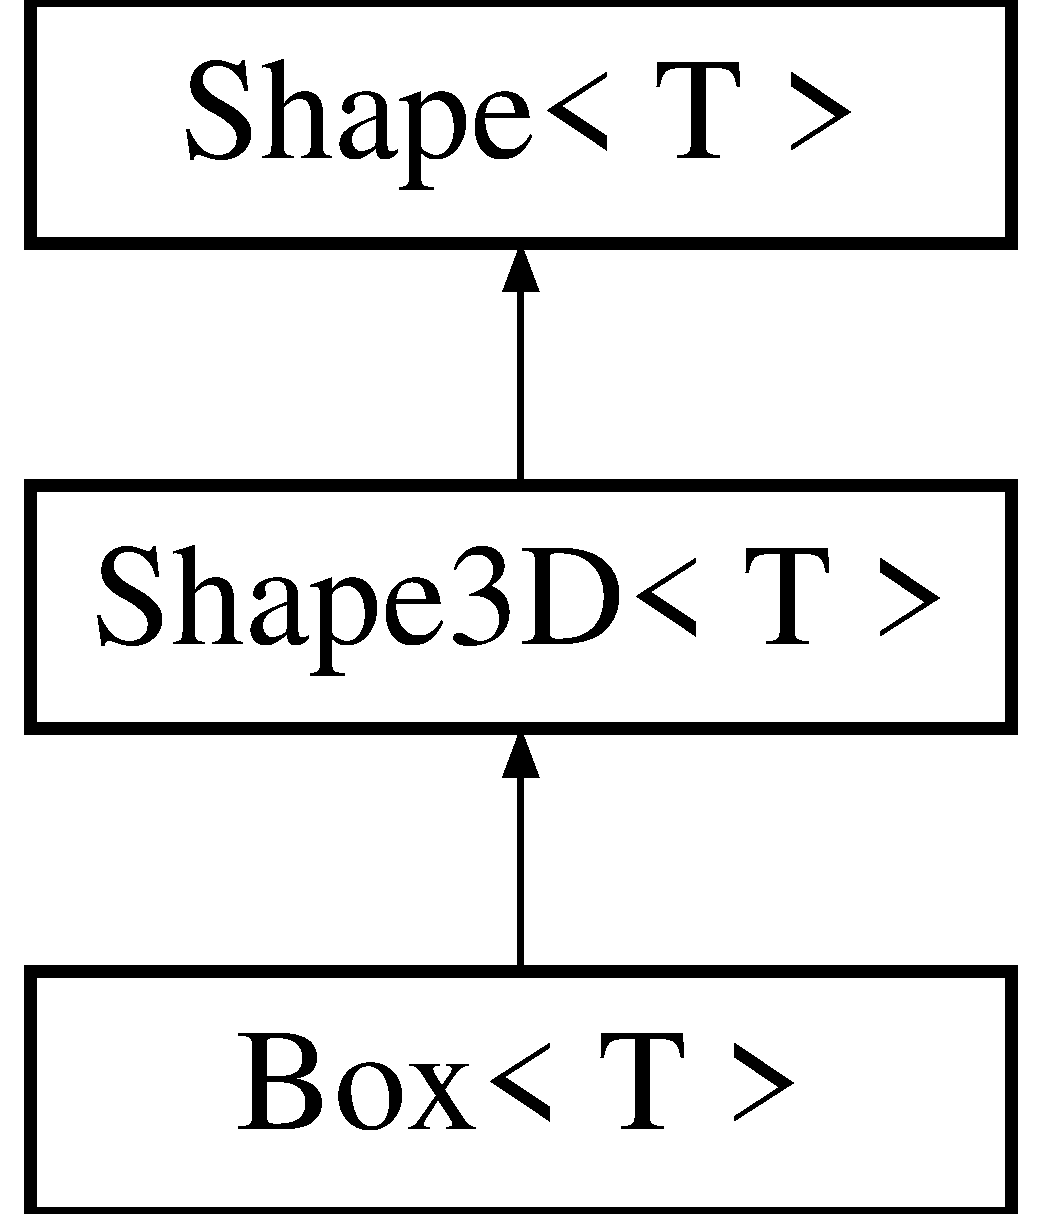
\includegraphics[height=3.000000cm]{classBox}
\end{center}
\end{figure}
\subsection*{Public Member Functions}
\begin{DoxyCompactItemize}
\item 
\mbox{\hyperlink{classBox_a057f84d8fa68647c6484d4e004d8ab74}{Box}} ()
\begin{DoxyCompactList}\small\item\em \mbox{\hyperlink{classA}{A}} basic constructor. \end{DoxyCompactList}\item 
\mbox{\hyperlink{classBox_af72b67fa2f421acbe9a7d3d1bcd540d1}{Box}} (\mbox{\hyperlink{classBox}{Box}} \&\&)=default
\item 
\mbox{\hyperlink{classBox}{Box}} \& \mbox{\hyperlink{classBox_a09995e3360b336b8a477d84804a5a70d}{operator=}} (\mbox{\hyperlink{classBox}{Box}} \&\&)=default
\item 
\mbox{\hyperlink{classBox_aab49a6687d04530ec60421bcbdb929c2}{Box}} (const \mbox{\hyperlink{classBox}{Box}} \&)=default
\item 
\mbox{\hyperlink{classBox}{Box}} \& \mbox{\hyperlink{classBox_a6ea0d233bdcce789b46384d22601da8d}{operator=}} (const \mbox{\hyperlink{classBox}{Box}} \&)=default
\item 
float \mbox{\hyperlink{classBox_ac64e9d619b0f3b991174a2ac49fef899}{perimeter}} ()
\end{DoxyCompactItemize}
\subsection*{Private Member Functions}
\begin{DoxyCompactItemize}
\item 
void \mbox{\hyperlink{classBox_a7f7b061bf913f9ab47bff75536bc137d}{generate\+\_\+vertexes}} ()
\begin{DoxyCompactList}\small\item\em \mbox{\hyperlink{classThis}{This}} function sets the correct vertexes. \end{DoxyCompactList}\end{DoxyCompactItemize}
\subsection*{Additional Inherited Members}


\subsection{Detailed Description}
\subsubsection*{template$<$typename T$>$\newline
class Box$<$ T $>$}

3D box shape. 

\subsection{Constructor \& Destructor Documentation}
\mbox{\Hypertarget{classBox_a057f84d8fa68647c6484d4e004d8ab74}\label{classBox_a057f84d8fa68647c6484d4e004d8ab74}} 
\index{Box@{Box}!Box@{Box}}
\index{Box@{Box}!Box@{Box}}
\subsubsection{\texorpdfstring{Box()}{Box()}\hspace{0.1cm}{\footnotesize\ttfamily [1/3]}}
{\footnotesize\ttfamily template$<$typename T $>$ \\
\mbox{\hyperlink{classBox}{Box}}$<$ T $>$\+::\mbox{\hyperlink{classBox}{Box}} (\begin{DoxyParamCaption}{ }\end{DoxyParamCaption})}



\mbox{\hyperlink{classA}{A}} basic constructor. 

The constructor generates vertexes and initializes buffers \mbox{\Hypertarget{classBox_af72b67fa2f421acbe9a7d3d1bcd540d1}\label{classBox_af72b67fa2f421acbe9a7d3d1bcd540d1}} 
\index{Box@{Box}!Box@{Box}}
\index{Box@{Box}!Box@{Box}}
\subsubsection{\texorpdfstring{Box()}{Box()}\hspace{0.1cm}{\footnotesize\ttfamily [2/3]}}
{\footnotesize\ttfamily template$<$typename T$>$ \\
\mbox{\hyperlink{classBox}{Box}}$<$ T $>$\+::\mbox{\hyperlink{classBox}{Box}} (\begin{DoxyParamCaption}\item[{\mbox{\hyperlink{classBox}{Box}}$<$ T $>$ \&\&}]{ }\end{DoxyParamCaption})\hspace{0.3cm}{\ttfamily [default]}}

\mbox{\Hypertarget{classBox_aab49a6687d04530ec60421bcbdb929c2}\label{classBox_aab49a6687d04530ec60421bcbdb929c2}} 
\index{Box@{Box}!Box@{Box}}
\index{Box@{Box}!Box@{Box}}
\subsubsection{\texorpdfstring{Box()}{Box()}\hspace{0.1cm}{\footnotesize\ttfamily [3/3]}}
{\footnotesize\ttfamily template$<$typename T$>$ \\
\mbox{\hyperlink{classBox}{Box}}$<$ T $>$\+::\mbox{\hyperlink{classBox}{Box}} (\begin{DoxyParamCaption}\item[{const \mbox{\hyperlink{classBox}{Box}}$<$ T $>$ \&}]{ }\end{DoxyParamCaption})\hspace{0.3cm}{\ttfamily [default]}}



\subsection{Member Function Documentation}
\mbox{\Hypertarget{classBox_a7f7b061bf913f9ab47bff75536bc137d}\label{classBox_a7f7b061bf913f9ab47bff75536bc137d}} 
\index{Box@{Box}!generate\+\_\+vertexes@{generate\+\_\+vertexes}}
\index{generate\+\_\+vertexes@{generate\+\_\+vertexes}!Box@{Box}}
\subsubsection{\texorpdfstring{generate\+\_\+vertexes()}{generate\_vertexes()}}
{\footnotesize\ttfamily template$<$typename T $>$ \\
void \mbox{\hyperlink{classBox}{Box}}$<$ T $>$\+::generate\+\_\+vertexes (\begin{DoxyParamCaption}{ }\end{DoxyParamCaption})\hspace{0.3cm}{\ttfamily [private]}}



\mbox{\hyperlink{classThis}{This}} function sets the correct vertexes. 

\mbox{\Hypertarget{classBox_a09995e3360b336b8a477d84804a5a70d}\label{classBox_a09995e3360b336b8a477d84804a5a70d}} 
\index{Box@{Box}!operator=@{operator=}}
\index{operator=@{operator=}!Box@{Box}}
\subsubsection{\texorpdfstring{operator=()}{operator=()}\hspace{0.1cm}{\footnotesize\ttfamily [1/2]}}
{\footnotesize\ttfamily template$<$typename T$>$ \\
\mbox{\hyperlink{classBox}{Box}}\& \mbox{\hyperlink{classBox}{Box}}$<$ T $>$\+::operator= (\begin{DoxyParamCaption}\item[{\mbox{\hyperlink{classBox}{Box}}$<$ T $>$ \&\&}]{ }\end{DoxyParamCaption})\hspace{0.3cm}{\ttfamily [default]}}

\mbox{\Hypertarget{classBox_a6ea0d233bdcce789b46384d22601da8d}\label{classBox_a6ea0d233bdcce789b46384d22601da8d}} 
\index{Box@{Box}!operator=@{operator=}}
\index{operator=@{operator=}!Box@{Box}}
\subsubsection{\texorpdfstring{operator=()}{operator=()}\hspace{0.1cm}{\footnotesize\ttfamily [2/2]}}
{\footnotesize\ttfamily template$<$typename T$>$ \\
\mbox{\hyperlink{classBox}{Box}}\& \mbox{\hyperlink{classBox}{Box}}$<$ T $>$\+::operator= (\begin{DoxyParamCaption}\item[{const \mbox{\hyperlink{classBox}{Box}}$<$ T $>$ \&}]{ }\end{DoxyParamCaption})\hspace{0.3cm}{\ttfamily [default]}}

\mbox{\Hypertarget{classBox_ac64e9d619b0f3b991174a2ac49fef899}\label{classBox_ac64e9d619b0f3b991174a2ac49fef899}} 
\index{Box@{Box}!perimeter@{perimeter}}
\index{perimeter@{perimeter}!Box@{Box}}
\subsubsection{\texorpdfstring{perimeter()}{perimeter()}}
{\footnotesize\ttfamily template$<$typename T$>$ \\
float \mbox{\hyperlink{classBox}{Box}}$<$ T $>$\+::perimeter (\begin{DoxyParamCaption}{ }\end{DoxyParamCaption})}



The documentation for this class was generated from the following file\+:\begin{DoxyCompactItemize}
\item 
src/shapes/\mbox{\hyperlink{box_8hpp}{box.\+hpp}}\end{DoxyCompactItemize}

\hypertarget{classCircle}{}\section{Circle$<$ T $>$ Class Template Reference}
\label{classCircle}\index{Circle$<$ T $>$@{Circle$<$ T $>$}}


{\ttfamily \#include \char`\"{}circle.\+hpp\char`\"{}}

Inheritance diagram for Circle$<$ T $>$\+:\begin{figure}[H]
\begin{center}
\leavevmode
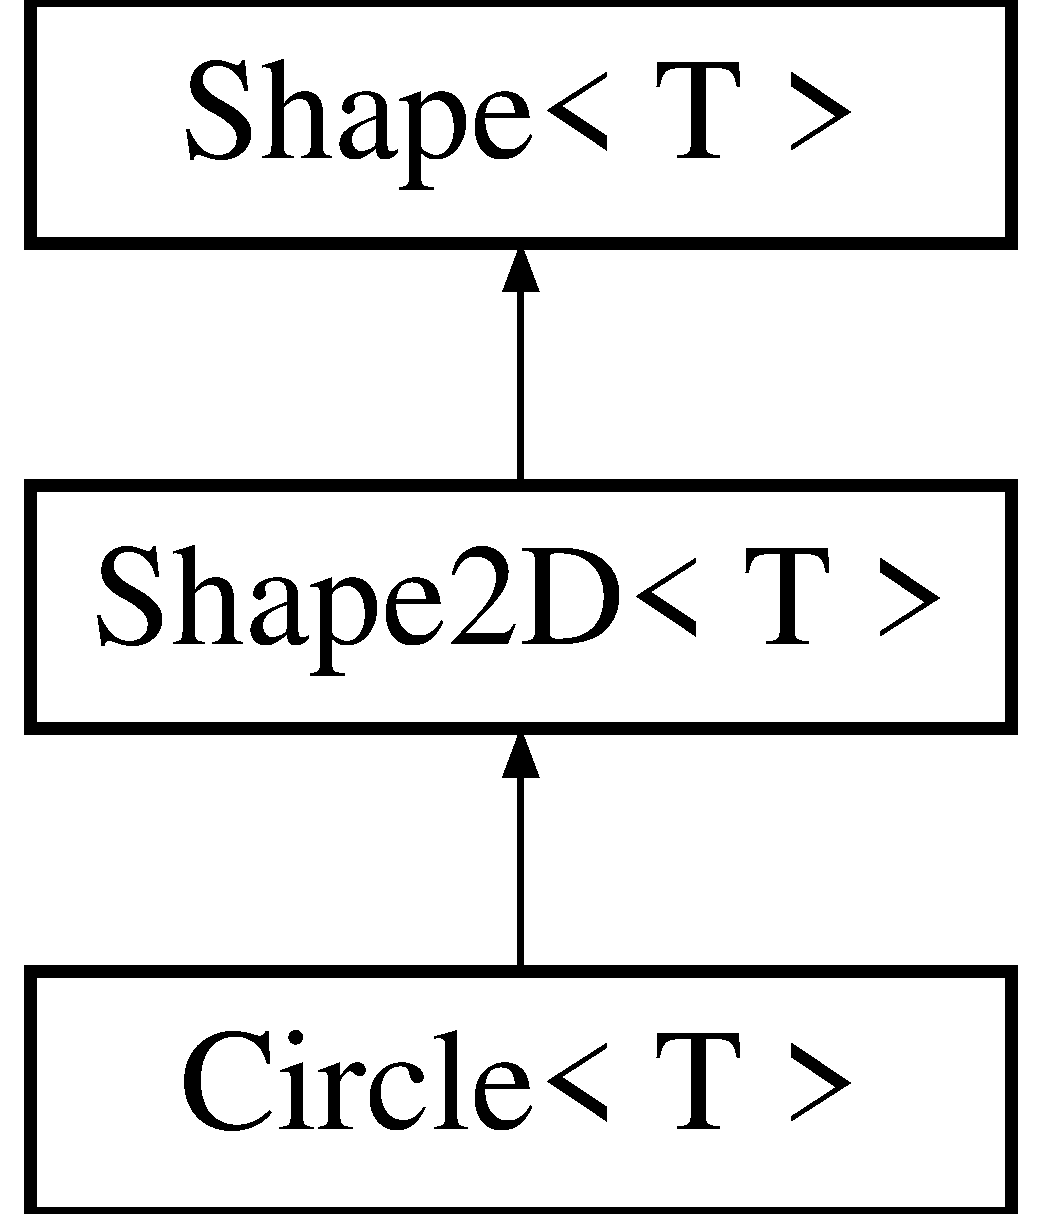
\includegraphics[height=3.000000cm]{classCircle}
\end{center}
\end{figure}
\subsection*{Public Member Functions}
\begin{DoxyCompactItemize}
\item 
\mbox{\hyperlink{classCircle_a0a298ea0e982a94a60091aeb2767f6e4}{Circle}} ()
\begin{DoxyCompactList}\small\item\em Basic constructor for class \mbox{\hyperlink{classCircle}{Circle}}. \end{DoxyCompactList}\item 
\mbox{\hyperlink{classCircle_ad4ee8eadfd4201a937af204ac4e6ec37}{Circle}} (\mbox{\hyperlink{classCircle}{Circle}} \&\&)=default
\item 
\mbox{\hyperlink{classCircle}{Circle}} \& \mbox{\hyperlink{classCircle_a06c8a2624fa51b38023e0326e8ccf789}{operator=}} (\mbox{\hyperlink{classCircle}{Circle}} \&\&)=default
\item 
\mbox{\hyperlink{classCircle_a163162aa8beaceb25ebd9a17966f4bd5}{Circle}} (const \mbox{\hyperlink{classCircle}{Circle}} \&)=default
\item 
\mbox{\hyperlink{classCircle}{Circle}} \& \mbox{\hyperlink{classCircle_a0e3ef62951a8fccaf0635ea21ae73eca}{operator=}} (const \mbox{\hyperlink{classCircle}{Circle}} \&)=default
\item 
T \mbox{\hyperlink{classCircle_a6f066fc39c0de339b0498b04a56be028}{perimeter}} ()
\item 
{\footnotesize template$<$$>$ }\\float \mbox{\hyperlink{classCircle_aa6c86a4a5d3ee7eb598879ba856430d9}{perimeter}} ()
\begin{DoxyCompactList}\small\item\em \mbox{\hyperlink{classThis}{This}} function calculates perimeter of a circle with radius 1. \end{DoxyCompactList}\end{DoxyCompactItemize}
\subsection*{Private Member Functions}
\begin{DoxyCompactItemize}
\item 
void \mbox{\hyperlink{classCircle_a07ce44d6b3a70ee7cbcf19e02e50c361}{generate\+\_\+vertexes}} (int=-\/1)
\item 
{\footnotesize template$<$$>$ }\\void \mbox{\hyperlink{classCircle_a5c5d9e9bf7ddada0681ad6977e4469f6}{generate\+\_\+vertexes}} (int num\+\_\+vert)
\begin{DoxyCompactList}\small\item\em \mbox{\hyperlink{classThis}{This}} function generates vertexes for float version of class \mbox{\hyperlink{classCircle}{Circle}}. \end{DoxyCompactList}\end{DoxyCompactItemize}
\subsection*{Additional Inherited Members}


\subsection{Constructor \& Destructor Documentation}
\mbox{\Hypertarget{classCircle_a0a298ea0e982a94a60091aeb2767f6e4}\label{classCircle_a0a298ea0e982a94a60091aeb2767f6e4}} 
\index{Circle@{Circle}!Circle@{Circle}}
\index{Circle@{Circle}!Circle@{Circle}}
\subsubsection{\texorpdfstring{Circle()}{Circle()}\hspace{0.1cm}{\footnotesize\ttfamily [1/3]}}
{\footnotesize\ttfamily template$<$typename T $>$ \\
\mbox{\hyperlink{classCircle}{Circle}}$<$ T $>$\+::\mbox{\hyperlink{classCircle}{Circle}} (\begin{DoxyParamCaption}{ }\end{DoxyParamCaption})}



Basic constructor for class \mbox{\hyperlink{classCircle}{Circle}}. 

Constructor generates vertexes and initializes opengl buffers. \mbox{\Hypertarget{classCircle_ad4ee8eadfd4201a937af204ac4e6ec37}\label{classCircle_ad4ee8eadfd4201a937af204ac4e6ec37}} 
\index{Circle@{Circle}!Circle@{Circle}}
\index{Circle@{Circle}!Circle@{Circle}}
\subsubsection{\texorpdfstring{Circle()}{Circle()}\hspace{0.1cm}{\footnotesize\ttfamily [2/3]}}
{\footnotesize\ttfamily template$<$typename T  = float$>$ \\
\mbox{\hyperlink{classCircle}{Circle}}$<$ T $>$\+::\mbox{\hyperlink{classCircle}{Circle}} (\begin{DoxyParamCaption}\item[{\mbox{\hyperlink{classCircle}{Circle}}$<$ T $>$ \&\&}]{ }\end{DoxyParamCaption})\hspace{0.3cm}{\ttfamily [default]}}

\mbox{\Hypertarget{classCircle_a163162aa8beaceb25ebd9a17966f4bd5}\label{classCircle_a163162aa8beaceb25ebd9a17966f4bd5}} 
\index{Circle@{Circle}!Circle@{Circle}}
\index{Circle@{Circle}!Circle@{Circle}}
\subsubsection{\texorpdfstring{Circle()}{Circle()}\hspace{0.1cm}{\footnotesize\ttfamily [3/3]}}
{\footnotesize\ttfamily template$<$typename T  = float$>$ \\
\mbox{\hyperlink{classCircle}{Circle}}$<$ T $>$\+::\mbox{\hyperlink{classCircle}{Circle}} (\begin{DoxyParamCaption}\item[{const \mbox{\hyperlink{classCircle}{Circle}}$<$ T $>$ \&}]{ }\end{DoxyParamCaption})\hspace{0.3cm}{\ttfamily [default]}}



\subsection{Member Function Documentation}
\mbox{\Hypertarget{classCircle_a07ce44d6b3a70ee7cbcf19e02e50c361}\label{classCircle_a07ce44d6b3a70ee7cbcf19e02e50c361}} 
\index{Circle@{Circle}!generate\+\_\+vertexes@{generate\+\_\+vertexes}}
\index{generate\+\_\+vertexes@{generate\+\_\+vertexes}!Circle@{Circle}}
\subsubsection{\texorpdfstring{generate\+\_\+vertexes()}{generate\_vertexes()}\hspace{0.1cm}{\footnotesize\ttfamily [1/2]}}
{\footnotesize\ttfamily template$<$typename T  = float$>$ \\
void \mbox{\hyperlink{classCircle}{Circle}}$<$ T $>$\+::generate\+\_\+vertexes (\begin{DoxyParamCaption}\item[{int}]{ = {\ttfamily -\/1} }\end{DoxyParamCaption})\hspace{0.3cm}{\ttfamily [private]}}

\mbox{\Hypertarget{classCircle_a5c5d9e9bf7ddada0681ad6977e4469f6}\label{classCircle_a5c5d9e9bf7ddada0681ad6977e4469f6}} 
\index{Circle@{Circle}!generate\+\_\+vertexes@{generate\+\_\+vertexes}}
\index{generate\+\_\+vertexes@{generate\+\_\+vertexes}!Circle@{Circle}}
\subsubsection{\texorpdfstring{generate\+\_\+vertexes()}{generate\_vertexes()}\hspace{0.1cm}{\footnotesize\ttfamily [2/2]}}
{\footnotesize\ttfamily template$<$$>$ \\
void \mbox{\hyperlink{classCircle}{Circle}}$<$ float $>$\+::generate\+\_\+vertexes (\begin{DoxyParamCaption}\item[{int}]{num\+\_\+vert }\end{DoxyParamCaption})\hspace{0.3cm}{\ttfamily [inline]}, {\ttfamily [private]}}



\mbox{\hyperlink{classThis}{This}} function generates vertexes for float version of class \mbox{\hyperlink{classCircle}{Circle}}. 

Internally, it uses sse instructions -\/ cpu support needed. \mbox{\Hypertarget{classCircle_a06c8a2624fa51b38023e0326e8ccf789}\label{classCircle_a06c8a2624fa51b38023e0326e8ccf789}} 
\index{Circle@{Circle}!operator=@{operator=}}
\index{operator=@{operator=}!Circle@{Circle}}
\subsubsection{\texorpdfstring{operator=()}{operator=()}\hspace{0.1cm}{\footnotesize\ttfamily [1/2]}}
{\footnotesize\ttfamily template$<$typename T  = float$>$ \\
\mbox{\hyperlink{classCircle}{Circle}}\& \mbox{\hyperlink{classCircle}{Circle}}$<$ T $>$\+::operator= (\begin{DoxyParamCaption}\item[{\mbox{\hyperlink{classCircle}{Circle}}$<$ T $>$ \&\&}]{ }\end{DoxyParamCaption})\hspace{0.3cm}{\ttfamily [default]}}

\mbox{\Hypertarget{classCircle_a0e3ef62951a8fccaf0635ea21ae73eca}\label{classCircle_a0e3ef62951a8fccaf0635ea21ae73eca}} 
\index{Circle@{Circle}!operator=@{operator=}}
\index{operator=@{operator=}!Circle@{Circle}}
\subsubsection{\texorpdfstring{operator=()}{operator=()}\hspace{0.1cm}{\footnotesize\ttfamily [2/2]}}
{\footnotesize\ttfamily template$<$typename T  = float$>$ \\
\mbox{\hyperlink{classCircle}{Circle}}\& \mbox{\hyperlink{classCircle}{Circle}}$<$ T $>$\+::operator= (\begin{DoxyParamCaption}\item[{const \mbox{\hyperlink{classCircle}{Circle}}$<$ T $>$ \&}]{ }\end{DoxyParamCaption})\hspace{0.3cm}{\ttfamily [default]}}

\mbox{\Hypertarget{classCircle_a6f066fc39c0de339b0498b04a56be028}\label{classCircle_a6f066fc39c0de339b0498b04a56be028}} 
\index{Circle@{Circle}!perimeter@{perimeter}}
\index{perimeter@{perimeter}!Circle@{Circle}}
\subsubsection{\texorpdfstring{perimeter()}{perimeter()}\hspace{0.1cm}{\footnotesize\ttfamily [1/2]}}
{\footnotesize\ttfamily template$<$typename T  = float$>$ \\
T \mbox{\hyperlink{classCircle}{Circle}}$<$ T $>$\+::perimeter (\begin{DoxyParamCaption}{ }\end{DoxyParamCaption})}

\mbox{\Hypertarget{classCircle_aa6c86a4a5d3ee7eb598879ba856430d9}\label{classCircle_aa6c86a4a5d3ee7eb598879ba856430d9}} 
\index{Circle@{Circle}!perimeter@{perimeter}}
\index{perimeter@{perimeter}!Circle@{Circle}}
\subsubsection{\texorpdfstring{perimeter()}{perimeter()}\hspace{0.1cm}{\footnotesize\ttfamily [2/2]}}
{\footnotesize\ttfamily template$<$$>$ \\
float \mbox{\hyperlink{classCircle}{Circle}}$<$ float $>$\+::perimeter (\begin{DoxyParamCaption}{ }\end{DoxyParamCaption})\hspace{0.3cm}{\ttfamily [inline]}}



\mbox{\hyperlink{classThis}{This}} function calculates perimeter of a circle with radius 1. 

Internally, it uses sse instructions -\/ cpu support needed. 

The documentation for this class was generated from the following file\+:\begin{DoxyCompactItemize}
\item 
src/shapes/\mbox{\hyperlink{circle_8hpp}{circle.\+hpp}}\end{DoxyCompactItemize}

\hypertarget{classDisk}{}\section{Disk$<$ T $>$ Class Template Reference}
\label{classDisk}\index{Disk$<$ T $>$@{Disk$<$ T $>$}}


\mbox{\hyperlink{classA}{A}} class holding vertexes in the shape of a disk.  




{\ttfamily \#include \char`\"{}disk.\+hpp\char`\"{}}

Inheritance diagram for Disk$<$ T $>$\+:\begin{figure}[H]
\begin{center}
\leavevmode
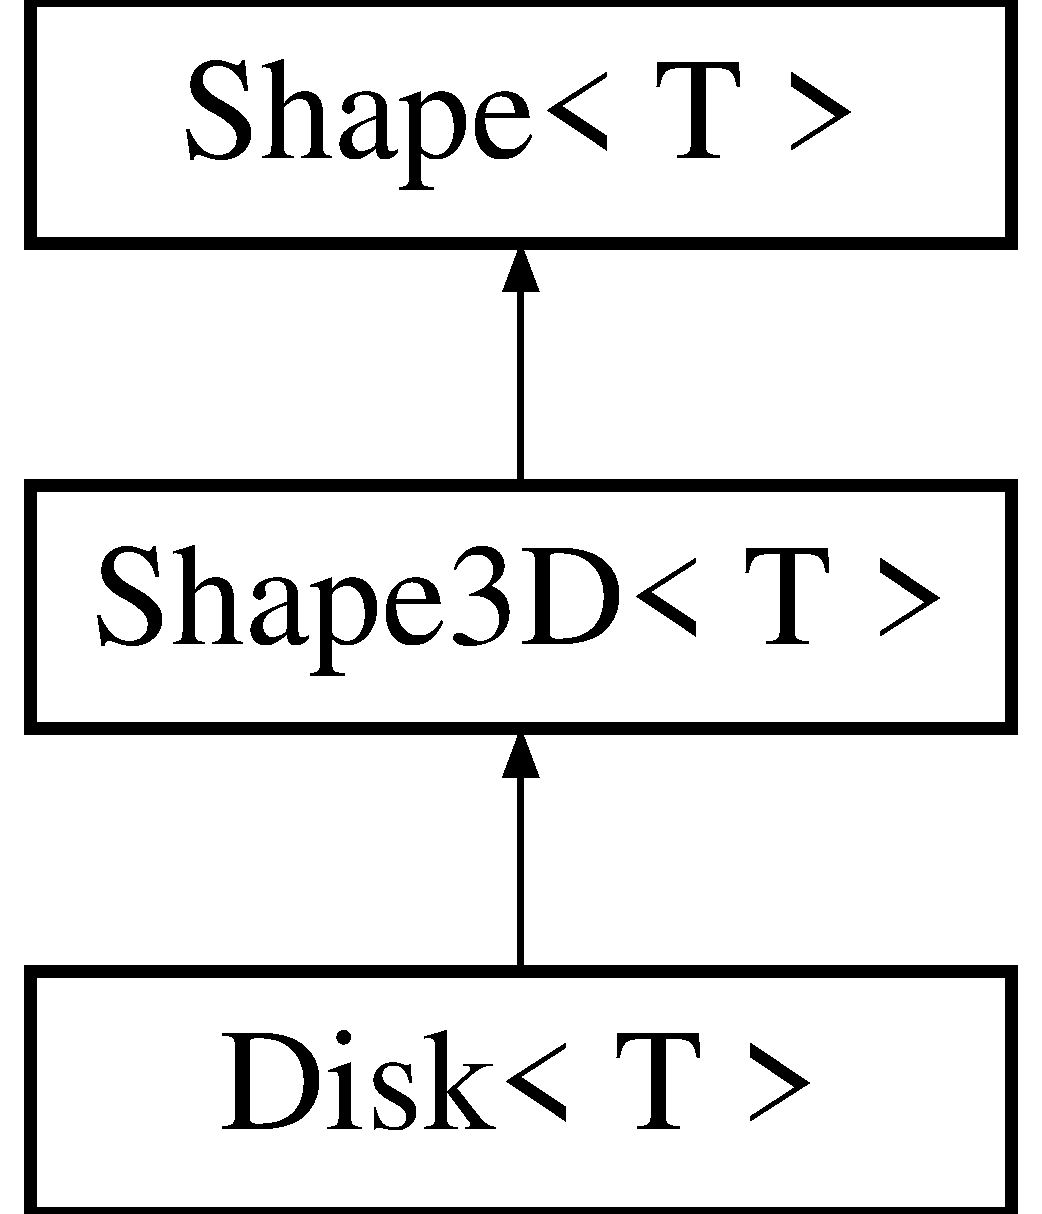
\includegraphics[height=3.000000cm]{classDisk}
\end{center}
\end{figure}
\subsection*{Public Member Functions}
\begin{DoxyCompactItemize}
\item 
\mbox{\hyperlink{classDisk_a88bcdb9bf91c8e9c18cdf551e558ab8c}{Disk}} ()
\begin{DoxyCompactList}\small\item\em \mbox{\hyperlink{classA}{A}} basic constructor. \end{DoxyCompactList}\item 
\mbox{\hyperlink{classDisk_af73e1930d8da87b05c813814532dd43a}{Disk}} (int, T=0.\+5)
\item 
\mbox{\hyperlink{classDisk_a893da931e3f39c126c434ab2fc2e12cc}{Disk}} (\mbox{\hyperlink{classDisk}{Disk}} \&\&)=default
\item 
\mbox{\hyperlink{classDisk}{Disk}} \& \mbox{\hyperlink{classDisk_ad6bc474ffecbc5de6f8fdd90ba5eddfe}{operator=}} (\mbox{\hyperlink{classDisk}{Disk}} \&\&)=default
\item 
\mbox{\hyperlink{classDisk_a96de79b2e115c478a33cc31f4818aee9}{Disk}} (const \mbox{\hyperlink{classDisk}{Disk}} \&)=default
\item 
\mbox{\hyperlink{classDisk}{Disk}} \& \mbox{\hyperlink{classDisk_a3ef862dd6e4671c907e2368bb5239bd2}{operator=}} (const \mbox{\hyperlink{classDisk}{Disk}} \&)=default
\end{DoxyCompactItemize}
\subsection*{Private Member Functions}
\begin{DoxyCompactItemize}
\item 
void \mbox{\hyperlink{classDisk_a1588532798901180b1eef6f3e1fb83f6}{generate\+\_\+vertexes}} ()
\item 
void \mbox{\hyperlink{classDisk_a4637847208b7236010085ca67f49e39a}{generate\+\_\+wheel\+\_\+line\+\_\+elements}} ()
\begin{DoxyCompactList}\small\item\em Function which generates sets wheel elements. Render wheel elements array with G\+L\+\_\+\+L\+I\+N\+ES to draw a wheel. \end{DoxyCompactList}\item 
{\footnotesize template$<$$>$ }\\void \mbox{\hyperlink{classDisk_a55648a13c42982087f60742da15c2c41}{generate\+\_\+vertexes}} ()
\begin{DoxyCompactList}\small\item\em Function which generates vertexes for float version of this class. \end{DoxyCompactList}\end{DoxyCompactItemize}
\subsection*{Private Attributes}
\begin{DoxyCompactItemize}
\item 
std\+::vector$<$ int $>$ \mbox{\hyperlink{classDisk_aa008e8bd0e7acdb4a1a56a8f44f048d7}{wheel\+\_\+line\+\_\+elements}}
\end{DoxyCompactItemize}
\subsection*{Additional Inherited Members}


\subsection{Detailed Description}
\subsubsection*{template$<$typename T = float$>$\newline
class Disk$<$ T $>$}

\mbox{\hyperlink{classA}{A}} class holding vertexes in the shape of a disk. 

\mbox{\hyperlink{classA}{A}} class holding vertexes in the shape of a disk. \mbox{\hyperlink{classDisk}{Disk}} is a 3d shape, thus it inherits from \mbox{\hyperlink{classShape3D}{Shape3D}} class. Template parameter can either be float or double. 
\begin{DoxyParams}{Parameters}
{\em T} & Template parameter T can either be float of double \\
\hline
\end{DoxyParams}


\subsection{Constructor \& Destructor Documentation}
\mbox{\Hypertarget{classDisk_a88bcdb9bf91c8e9c18cdf551e558ab8c}\label{classDisk_a88bcdb9bf91c8e9c18cdf551e558ab8c}} 
\index{Disk@{Disk}!Disk@{Disk}}
\index{Disk@{Disk}!Disk@{Disk}}
\subsubsection{\texorpdfstring{Disk()}{Disk()}\hspace{0.1cm}{\footnotesize\ttfamily [1/4]}}
{\footnotesize\ttfamily template$<$typename T $>$ \\
\mbox{\hyperlink{classDisk}{Disk}}$<$ T $>$\+::\mbox{\hyperlink{classDisk}{Disk}} (\begin{DoxyParamCaption}{ }\end{DoxyParamCaption})}



\mbox{\hyperlink{classA}{A}} basic constructor. 

Constructor initializes all important variables, geenratex necessary vertexes and initializes opengl buffers. \mbox{\Hypertarget{classDisk_af73e1930d8da87b05c813814532dd43a}\label{classDisk_af73e1930d8da87b05c813814532dd43a}} 
\index{Disk@{Disk}!Disk@{Disk}}
\index{Disk@{Disk}!Disk@{Disk}}
\subsubsection{\texorpdfstring{Disk()}{Disk()}\hspace{0.1cm}{\footnotesize\ttfamily [2/4]}}
{\footnotesize\ttfamily template$<$typename T  = float$>$ \\
\mbox{\hyperlink{classDisk}{Disk}}$<$ T $>$\+::\mbox{\hyperlink{classDisk}{Disk}} (\begin{DoxyParamCaption}\item[{int}]{,  }\item[{T}]{ = {\ttfamily 0.5} }\end{DoxyParamCaption})}

\mbox{\Hypertarget{classDisk_a893da931e3f39c126c434ab2fc2e12cc}\label{classDisk_a893da931e3f39c126c434ab2fc2e12cc}} 
\index{Disk@{Disk}!Disk@{Disk}}
\index{Disk@{Disk}!Disk@{Disk}}
\subsubsection{\texorpdfstring{Disk()}{Disk()}\hspace{0.1cm}{\footnotesize\ttfamily [3/4]}}
{\footnotesize\ttfamily template$<$typename T  = float$>$ \\
\mbox{\hyperlink{classDisk}{Disk}}$<$ T $>$\+::\mbox{\hyperlink{classDisk}{Disk}} (\begin{DoxyParamCaption}\item[{\mbox{\hyperlink{classDisk}{Disk}}$<$ T $>$ \&\&}]{ }\end{DoxyParamCaption})\hspace{0.3cm}{\ttfamily [default]}}

\mbox{\Hypertarget{classDisk_a96de79b2e115c478a33cc31f4818aee9}\label{classDisk_a96de79b2e115c478a33cc31f4818aee9}} 
\index{Disk@{Disk}!Disk@{Disk}}
\index{Disk@{Disk}!Disk@{Disk}}
\subsubsection{\texorpdfstring{Disk()}{Disk()}\hspace{0.1cm}{\footnotesize\ttfamily [4/4]}}
{\footnotesize\ttfamily template$<$typename T  = float$>$ \\
\mbox{\hyperlink{classDisk}{Disk}}$<$ T $>$\+::\mbox{\hyperlink{classDisk}{Disk}} (\begin{DoxyParamCaption}\item[{const \mbox{\hyperlink{classDisk}{Disk}}$<$ T $>$ \&}]{ }\end{DoxyParamCaption})\hspace{0.3cm}{\ttfamily [default]}}



\subsection{Member Function Documentation}
\mbox{\Hypertarget{classDisk_a1588532798901180b1eef6f3e1fb83f6}\label{classDisk_a1588532798901180b1eef6f3e1fb83f6}} 
\index{Disk@{Disk}!generate\+\_\+vertexes@{generate\+\_\+vertexes}}
\index{generate\+\_\+vertexes@{generate\+\_\+vertexes}!Disk@{Disk}}
\subsubsection{\texorpdfstring{generate\+\_\+vertexes()}{generate\_vertexes()}\hspace{0.1cm}{\footnotesize\ttfamily [1/2]}}
{\footnotesize\ttfamily template$<$typename T  = float$>$ \\
void \mbox{\hyperlink{classDisk}{Disk}}$<$ T $>$\+::generate\+\_\+vertexes (\begin{DoxyParamCaption}{ }\end{DoxyParamCaption})\hspace{0.3cm}{\ttfamily [private]}}

\mbox{\Hypertarget{classDisk_a55648a13c42982087f60742da15c2c41}\label{classDisk_a55648a13c42982087f60742da15c2c41}} 
\index{Disk@{Disk}!generate\+\_\+vertexes@{generate\+\_\+vertexes}}
\index{generate\+\_\+vertexes@{generate\+\_\+vertexes}!Disk@{Disk}}
\subsubsection{\texorpdfstring{generate\+\_\+vertexes()}{generate\_vertexes()}\hspace{0.1cm}{\footnotesize\ttfamily [2/2]}}
{\footnotesize\ttfamily template$<$$>$ \\
void \mbox{\hyperlink{classDisk}{Disk}}$<$ float $>$\+::generate\+\_\+vertexes (\begin{DoxyParamCaption}{ }\end{DoxyParamCaption})\hspace{0.3cm}{\ttfamily [inline]}, {\ttfamily [private]}}



Function which generates vertexes for float version of this class. 

Vertexes are generate in such a way that the middle of the shape is (0,0,0). The function also sets the element array. It uses sse instructions -\/ use appropriate processor. \mbox{\Hypertarget{classDisk_a4637847208b7236010085ca67f49e39a}\label{classDisk_a4637847208b7236010085ca67f49e39a}} 
\index{Disk@{Disk}!generate\+\_\+wheel\+\_\+line\+\_\+elements@{generate\+\_\+wheel\+\_\+line\+\_\+elements}}
\index{generate\+\_\+wheel\+\_\+line\+\_\+elements@{generate\+\_\+wheel\+\_\+line\+\_\+elements}!Disk@{Disk}}
\subsubsection{\texorpdfstring{generate\+\_\+wheel\+\_\+line\+\_\+elements()}{generate\_wheel\_line\_elements()}}
{\footnotesize\ttfamily template$<$typename T $>$ \\
void \mbox{\hyperlink{classDisk}{Disk}}$<$ T $>$\+::generate\+\_\+wheel\+\_\+line\+\_\+elements (\begin{DoxyParamCaption}{ }\end{DoxyParamCaption})\hspace{0.3cm}{\ttfamily [private]}}



Function which generates sets wheel elements. Render wheel elements array with G\+L\+\_\+\+L\+I\+N\+ES to draw a wheel. 

\mbox{\Hypertarget{classDisk_ad6bc474ffecbc5de6f8fdd90ba5eddfe}\label{classDisk_ad6bc474ffecbc5de6f8fdd90ba5eddfe}} 
\index{Disk@{Disk}!operator=@{operator=}}
\index{operator=@{operator=}!Disk@{Disk}}
\subsubsection{\texorpdfstring{operator=()}{operator=()}\hspace{0.1cm}{\footnotesize\ttfamily [1/2]}}
{\footnotesize\ttfamily template$<$typename T  = float$>$ \\
\mbox{\hyperlink{classDisk}{Disk}}\& \mbox{\hyperlink{classDisk}{Disk}}$<$ T $>$\+::operator= (\begin{DoxyParamCaption}\item[{\mbox{\hyperlink{classDisk}{Disk}}$<$ T $>$ \&\&}]{ }\end{DoxyParamCaption})\hspace{0.3cm}{\ttfamily [default]}}

\mbox{\Hypertarget{classDisk_a3ef862dd6e4671c907e2368bb5239bd2}\label{classDisk_a3ef862dd6e4671c907e2368bb5239bd2}} 
\index{Disk@{Disk}!operator=@{operator=}}
\index{operator=@{operator=}!Disk@{Disk}}
\subsubsection{\texorpdfstring{operator=()}{operator=()}\hspace{0.1cm}{\footnotesize\ttfamily [2/2]}}
{\footnotesize\ttfamily template$<$typename T  = float$>$ \\
\mbox{\hyperlink{classDisk}{Disk}}\& \mbox{\hyperlink{classDisk}{Disk}}$<$ T $>$\+::operator= (\begin{DoxyParamCaption}\item[{const \mbox{\hyperlink{classDisk}{Disk}}$<$ T $>$ \&}]{ }\end{DoxyParamCaption})\hspace{0.3cm}{\ttfamily [default]}}



\subsection{Member Data Documentation}
\mbox{\Hypertarget{classDisk_aa008e8bd0e7acdb4a1a56a8f44f048d7}\label{classDisk_aa008e8bd0e7acdb4a1a56a8f44f048d7}} 
\index{Disk@{Disk}!wheel\+\_\+line\+\_\+elements@{wheel\+\_\+line\+\_\+elements}}
\index{wheel\+\_\+line\+\_\+elements@{wheel\+\_\+line\+\_\+elements}!Disk@{Disk}}
\subsubsection{\texorpdfstring{wheel\+\_\+line\+\_\+elements}{wheel\_line\_elements}}
{\footnotesize\ttfamily template$<$typename T  = float$>$ \\
std\+::vector$<$int$>$ \mbox{\hyperlink{classDisk}{Disk}}$<$ T $>$\+::wheel\+\_\+line\+\_\+elements\hspace{0.3cm}{\ttfamily [private]}}

elements which determine wheel shape 

The documentation for this class was generated from the following file\+:\begin{DoxyCompactItemize}
\item 
src/\mbox{\hyperlink{disk_8hpp}{disk.\+hpp}}\end{DoxyCompactItemize}

\hypertarget{structstd_1_1hash_3_01pair_3_01S_00_01T_01_4_01_4}{}\section{std\+:\+:hash$<$ pair$<$ S, T $>$ $>$ Struct Template Reference}
\label{structstd_1_1hash_3_01pair_3_01S_00_01T_01_4_01_4}\index{std\+::hash$<$ pair$<$ S, T $>$ $>$@{std\+::hash$<$ pair$<$ S, T $>$ $>$}}


{\ttfamily \#include \char`\"{}auxiliary\+\_\+functions.\+hpp\char`\"{}}

\subsection*{Public Member Functions}
\begin{DoxyCompactItemize}
\item 
size\+\_\+t \mbox{\hyperlink{structstd_1_1hash_3_01pair_3_01S_00_01T_01_4_01_4_a6fec6cb26e96fb20d4ec121487e5acb4}{operator()}} (const pair$<$ S, T $>$ \&\mbox{\hyperlink{glad_8h_a30522dbcc3e66083fcf2bf64d1fad76a}{v}}) const
\end{DoxyCompactItemize}


\subsection{Member Function Documentation}
\mbox{\Hypertarget{structstd_1_1hash_3_01pair_3_01S_00_01T_01_4_01_4_a6fec6cb26e96fb20d4ec121487e5acb4}\label{structstd_1_1hash_3_01pair_3_01S_00_01T_01_4_01_4_a6fec6cb26e96fb20d4ec121487e5acb4}} 
\index{std\+::hash$<$ pair$<$ S, T $>$ $>$@{std\+::hash$<$ pair$<$ S, T $>$ $>$}!operator()@{operator()}}
\index{operator()@{operator()}!std\+::hash$<$ pair$<$ S, T $>$ $>$@{std\+::hash$<$ pair$<$ S, T $>$ $>$}}
\subsubsection{\texorpdfstring{operator()()}{operator()()}}
{\footnotesize\ttfamily template$<$typename S , typename T $>$ \\
size\+\_\+t std\+::hash$<$ pair$<$ S, T $>$ $>$\+::operator() (\begin{DoxyParamCaption}\item[{const pair$<$ S, T $>$ \&}]{v }\end{DoxyParamCaption}) const\hspace{0.3cm}{\ttfamily [inline]}}



The documentation for this struct was generated from the following file\+:\begin{DoxyCompactItemize}
\item 
src/algorithms/\mbox{\hyperlink{auxiliary__functions_8hpp}{auxiliary\+\_\+functions.\+hpp}}\end{DoxyCompactItemize}

\hypertarget{classRectangle}{}\section{Rectangle$<$ T $>$ Class Template Reference}
\label{classRectangle}\index{Rectangle$<$ T $>$@{Rectangle$<$ T $>$}}


Class holding rectangle vertexes.  




{\ttfamily \#include \char`\"{}rectangle.\+hpp\char`\"{}}

Inheritance diagram for Rectangle$<$ T $>$\+:\begin{figure}[H]
\begin{center}
\leavevmode
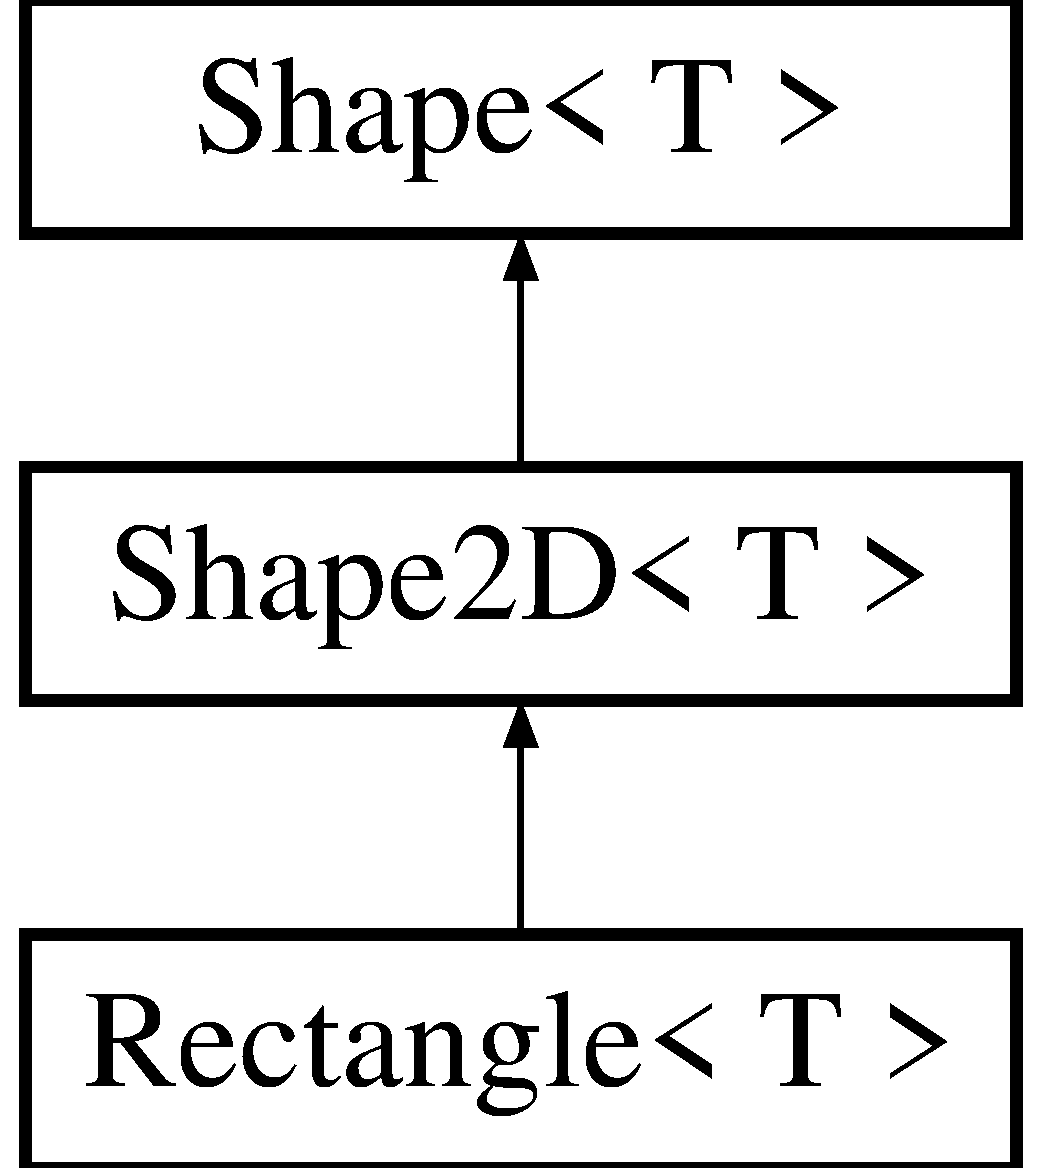
\includegraphics[height=3.000000cm]{classRectangle}
\end{center}
\end{figure}
\subsection*{Public Member Functions}
\begin{DoxyCompactItemize}
\item 
\mbox{\hyperlink{classRectangle_a9d9da3fc8bcb125516cbf2d711d325eb}{Rectangle}} ()
\begin{DoxyCompactList}\small\item\em \mbox{\hyperlink{classA}{A}} basic constructor. \end{DoxyCompactList}\item 
\mbox{\hyperlink{classRectangle_a34cf921863291153b40d9b447f812aa4}{Rectangle}} (\mbox{\hyperlink{classRectangle}{Rectangle}} \&\&)=default
\item 
\mbox{\hyperlink{classRectangle}{Rectangle}} \& \mbox{\hyperlink{classRectangle_ab53b617f14505834f525ec614ccce5c8}{operator=}} (\mbox{\hyperlink{classRectangle}{Rectangle}} \&\&)=default
\item 
\mbox{\hyperlink{classRectangle_acf27dae8f7c9a022428bda816903db2e}{Rectangle}} (const \mbox{\hyperlink{classRectangle}{Rectangle}} \&)=default
\item 
\mbox{\hyperlink{classRectangle}{Rectangle}} \& \mbox{\hyperlink{classRectangle_ad0a038c8959e5bde09bf1e8f49980bea}{operator=}} (const \mbox{\hyperlink{classRectangle}{Rectangle}} \&)=default
\item 
T \mbox{\hyperlink{classRectangle_a9c59dcb7376296711ad86e2da924d3c8}{perimeter}} ()
\end{DoxyCompactItemize}
\subsection*{Private Member Functions}
\begin{DoxyCompactItemize}
\item 
void \mbox{\hyperlink{classRectangle_a0f9d67fb9478883f067c47cdc7bf7bca}{generate\+\_\+vertexes}} ()
\begin{DoxyCompactList}\small\item\em Sets all four vertexes in correct order. \end{DoxyCompactList}\end{DoxyCompactItemize}
\subsection*{Additional Inherited Members}


\subsection{Detailed Description}
\subsubsection*{template$<$typename T = float$>$\newline
class Rectangle$<$ T $>$}

Class holding rectangle vertexes. 

\subsection{Constructor \& Destructor Documentation}
\mbox{\Hypertarget{classRectangle_a9d9da3fc8bcb125516cbf2d711d325eb}\label{classRectangle_a9d9da3fc8bcb125516cbf2d711d325eb}} 
\index{Rectangle@{Rectangle}!Rectangle@{Rectangle}}
\index{Rectangle@{Rectangle}!Rectangle@{Rectangle}}
\subsubsection{\texorpdfstring{Rectangle()}{Rectangle()}\hspace{0.1cm}{\footnotesize\ttfamily [1/3]}}
{\footnotesize\ttfamily template$<$typename T $>$ \\
\mbox{\hyperlink{classRectangle}{Rectangle}}$<$ T $>$\+::\mbox{\hyperlink{classRectangle}{Rectangle}} (\begin{DoxyParamCaption}{ }\end{DoxyParamCaption})}



\mbox{\hyperlink{classA}{A}} basic constructor. 

Constructor generates vertexes, initializes buffers and generates opengl buffers \mbox{\Hypertarget{classRectangle_a34cf921863291153b40d9b447f812aa4}\label{classRectangle_a34cf921863291153b40d9b447f812aa4}} 
\index{Rectangle@{Rectangle}!Rectangle@{Rectangle}}
\index{Rectangle@{Rectangle}!Rectangle@{Rectangle}}
\subsubsection{\texorpdfstring{Rectangle()}{Rectangle()}\hspace{0.1cm}{\footnotesize\ttfamily [2/3]}}
{\footnotesize\ttfamily template$<$typename T  = float$>$ \\
\mbox{\hyperlink{classRectangle}{Rectangle}}$<$ T $>$\+::\mbox{\hyperlink{classRectangle}{Rectangle}} (\begin{DoxyParamCaption}\item[{\mbox{\hyperlink{classRectangle}{Rectangle}}$<$ T $>$ \&\&}]{ }\end{DoxyParamCaption})\hspace{0.3cm}{\ttfamily [default]}}

\mbox{\Hypertarget{classRectangle_acf27dae8f7c9a022428bda816903db2e}\label{classRectangle_acf27dae8f7c9a022428bda816903db2e}} 
\index{Rectangle@{Rectangle}!Rectangle@{Rectangle}}
\index{Rectangle@{Rectangle}!Rectangle@{Rectangle}}
\subsubsection{\texorpdfstring{Rectangle()}{Rectangle()}\hspace{0.1cm}{\footnotesize\ttfamily [3/3]}}
{\footnotesize\ttfamily template$<$typename T  = float$>$ \\
\mbox{\hyperlink{classRectangle}{Rectangle}}$<$ T $>$\+::\mbox{\hyperlink{classRectangle}{Rectangle}} (\begin{DoxyParamCaption}\item[{const \mbox{\hyperlink{classRectangle}{Rectangle}}$<$ T $>$ \&}]{ }\end{DoxyParamCaption})\hspace{0.3cm}{\ttfamily [default]}}



\subsection{Member Function Documentation}
\mbox{\Hypertarget{classRectangle_a0f9d67fb9478883f067c47cdc7bf7bca}\label{classRectangle_a0f9d67fb9478883f067c47cdc7bf7bca}} 
\index{Rectangle@{Rectangle}!generate\+\_\+vertexes@{generate\+\_\+vertexes}}
\index{generate\+\_\+vertexes@{generate\+\_\+vertexes}!Rectangle@{Rectangle}}
\subsubsection{\texorpdfstring{generate\+\_\+vertexes()}{generate\_vertexes()}}
{\footnotesize\ttfamily template$<$typename T $>$ \\
void \mbox{\hyperlink{classRectangle}{Rectangle}}$<$ T $>$\+::generate\+\_\+vertexes (\begin{DoxyParamCaption}{ }\end{DoxyParamCaption})\hspace{0.3cm}{\ttfamily [private]}}



Sets all four vertexes in correct order. 

\mbox{\Hypertarget{classRectangle_ab53b617f14505834f525ec614ccce5c8}\label{classRectangle_ab53b617f14505834f525ec614ccce5c8}} 
\index{Rectangle@{Rectangle}!operator=@{operator=}}
\index{operator=@{operator=}!Rectangle@{Rectangle}}
\subsubsection{\texorpdfstring{operator=()}{operator=()}\hspace{0.1cm}{\footnotesize\ttfamily [1/2]}}
{\footnotesize\ttfamily template$<$typename T  = float$>$ \\
\mbox{\hyperlink{classRectangle}{Rectangle}}\& \mbox{\hyperlink{classRectangle}{Rectangle}}$<$ T $>$\+::operator= (\begin{DoxyParamCaption}\item[{\mbox{\hyperlink{classRectangle}{Rectangle}}$<$ T $>$ \&\&}]{ }\end{DoxyParamCaption})\hspace{0.3cm}{\ttfamily [default]}}

\mbox{\Hypertarget{classRectangle_ad0a038c8959e5bde09bf1e8f49980bea}\label{classRectangle_ad0a038c8959e5bde09bf1e8f49980bea}} 
\index{Rectangle@{Rectangle}!operator=@{operator=}}
\index{operator=@{operator=}!Rectangle@{Rectangle}}
\subsubsection{\texorpdfstring{operator=()}{operator=()}\hspace{0.1cm}{\footnotesize\ttfamily [2/2]}}
{\footnotesize\ttfamily template$<$typename T  = float$>$ \\
\mbox{\hyperlink{classRectangle}{Rectangle}}\& \mbox{\hyperlink{classRectangle}{Rectangle}}$<$ T $>$\+::operator= (\begin{DoxyParamCaption}\item[{const \mbox{\hyperlink{classRectangle}{Rectangle}}$<$ T $>$ \&}]{ }\end{DoxyParamCaption})\hspace{0.3cm}{\ttfamily [default]}}

\mbox{\Hypertarget{classRectangle_a9c59dcb7376296711ad86e2da924d3c8}\label{classRectangle_a9c59dcb7376296711ad86e2da924d3c8}} 
\index{Rectangle@{Rectangle}!perimeter@{perimeter}}
\index{perimeter@{perimeter}!Rectangle@{Rectangle}}
\subsubsection{\texorpdfstring{perimeter()}{perimeter()}}
{\footnotesize\ttfamily template$<$typename T $>$ \\
T \mbox{\hyperlink{classRectangle}{Rectangle}}$<$ T $>$\+::perimeter (\begin{DoxyParamCaption}{ }\end{DoxyParamCaption})}



The documentation for this class was generated from the following file\+:\begin{DoxyCompactItemize}
\item 
src/shapes/\mbox{\hyperlink{rectangle_8hpp}{rectangle.\+hpp}}\end{DoxyCompactItemize}

\hypertarget{classShader}{}\section{Shader$<$ T $>$ Class Template Reference}
\label{classShader}\index{Shader$<$ T $>$@{Shader$<$ T $>$}}


Class for shaders. \mbox{\hyperlink{classThis}{This}} class compiles three shaders, one for each dimension.  




{\ttfamily \#include \char`\"{}shader\+\_\+class.\+hpp\char`\"{}}

\subsection*{Public Member Functions}
\begin{DoxyCompactItemize}
\item 
\mbox{\hyperlink{classShader_a02faa1d7140779d7a24e06d1aff58d68}{Shader}} ()
\item 
\mbox{\hyperlink{classShader_a7e30078f161d1c9f48a7b3921c01f816}{Shader}} (\mbox{\hyperlink{classShader}{Shader}} \&\&)=delete
\item 
\mbox{\hyperlink{classShader}{Shader}} \& \mbox{\hyperlink{classShader_a3b92fece66095389581a2bf6b3124657}{operator=}} (\mbox{\hyperlink{classShader}{Shader}} \&\&)=delete
\item 
\mbox{\hyperlink{classShader_a49b2a448a00b5e1413c17501f8873cca}{Shader}} (const \mbox{\hyperlink{classShader}{Shader}} \&)=delete
\item 
\mbox{\hyperlink{classShader}{Shader}} \& \mbox{\hyperlink{classShader_a58f724fecccecdb1633e08ce0258da37}{operator=}} (const \mbox{\hyperlink{classShader}{Shader}} \&)=delete
\item 
unsigned \mbox{\hyperlink{classShader_a2c19b216850480109f9d5f7ed6ab6aa6}{get\+\_\+shader\+\_\+program}} (int i)
\end{DoxyCompactItemize}
\subsection*{Protected Member Functions}
\begin{DoxyCompactItemize}
\item 
void \mbox{\hyperlink{classShader_a1176d69a08aef6df3b7850104871a839}{compile\+\_\+shaders}} ()
\item 
{\footnotesize template$<$$>$ }\\void \mbox{\hyperlink{classShader_a3ffd553eceda4e9d5a1d8b4a5a157659}{compile\+\_\+shaders}} ()
\begin{DoxyCompactList}\small\item\em Constructor compiles shaders and tests them. \end{DoxyCompactList}\item 
{\footnotesize template$<$$>$ }\\void \mbox{\hyperlink{classShader_ae486635d367b6054482c56747ed74846}{compile\+\_\+shaders}} ()
\begin{DoxyCompactList}\small\item\em Constructor compiles shaders and tests them. \end{DoxyCompactList}\end{DoxyCompactItemize}
\subsection*{Protected Attributes}
\begin{DoxyCompactItemize}
\item 
unsigned \mbox{\hyperlink{classShader_af8ec4edd2b1b56f32ce416280ff9b9e1}{shader\+\_\+program}} \mbox{[}3\mbox{]}
\item 
bool \mbox{\hyperlink{classShader_a057162ea090f838f7fbb658cb301efc4}{shaders\+\_\+compiled}} \mbox{[}3\mbox{]}
\end{DoxyCompactItemize}


\subsection{Detailed Description}
\subsubsection*{template$<$R\+E\+N\+D\+E\+R\+\_\+\+T\+Y\+PE T$>$\newline
class Shader$<$ T $>$}

Class for shaders. \mbox{\hyperlink{classThis}{This}} class compiles three shaders, one for each dimension. 

Class can either be U\+N\+I\+F\+O\+R\+M\+\_\+\+C\+O\+L\+OR or C\+U\+S\+T\+O\+M\+\_\+\+C\+O\+L\+OR class. The difference is in shaders they compile. The first one compiles shader which assigns a single color to all vertexes. The latter assigns seprate color to each vertex. 

\subsection{Constructor \& Destructor Documentation}
\mbox{\Hypertarget{classShader_a02faa1d7140779d7a24e06d1aff58d68}\label{classShader_a02faa1d7140779d7a24e06d1aff58d68}} 
\index{Shader@{Shader}!Shader@{Shader}}
\index{Shader@{Shader}!Shader@{Shader}}
\subsubsection{\texorpdfstring{Shader()}{Shader()}\hspace{0.1cm}{\footnotesize\ttfamily [1/3]}}
{\footnotesize\ttfamily template$<$R\+E\+N\+D\+E\+R\+\_\+\+T\+Y\+PE T$>$ \\
\mbox{\hyperlink{classShader}{Shader}}$<$ T $>$\+::\mbox{\hyperlink{classShader}{Shader}} (\begin{DoxyParamCaption}{ }\end{DoxyParamCaption})\hspace{0.3cm}{\ttfamily [inline]}}

\mbox{\Hypertarget{classShader_a7e30078f161d1c9f48a7b3921c01f816}\label{classShader_a7e30078f161d1c9f48a7b3921c01f816}} 
\index{Shader@{Shader}!Shader@{Shader}}
\index{Shader@{Shader}!Shader@{Shader}}
\subsubsection{\texorpdfstring{Shader()}{Shader()}\hspace{0.1cm}{\footnotesize\ttfamily [2/3]}}
{\footnotesize\ttfamily template$<$R\+E\+N\+D\+E\+R\+\_\+\+T\+Y\+PE T$>$ \\
\mbox{\hyperlink{classShader}{Shader}}$<$ T $>$\+::\mbox{\hyperlink{classShader}{Shader}} (\begin{DoxyParamCaption}\item[{\mbox{\hyperlink{classShader}{Shader}}$<$ T $>$ \&\&}]{ }\end{DoxyParamCaption})\hspace{0.3cm}{\ttfamily [delete]}}

\mbox{\Hypertarget{classShader_a49b2a448a00b5e1413c17501f8873cca}\label{classShader_a49b2a448a00b5e1413c17501f8873cca}} 
\index{Shader@{Shader}!Shader@{Shader}}
\index{Shader@{Shader}!Shader@{Shader}}
\subsubsection{\texorpdfstring{Shader()}{Shader()}\hspace{0.1cm}{\footnotesize\ttfamily [3/3]}}
{\footnotesize\ttfamily template$<$R\+E\+N\+D\+E\+R\+\_\+\+T\+Y\+PE T$>$ \\
\mbox{\hyperlink{classShader}{Shader}}$<$ T $>$\+::\mbox{\hyperlink{classShader}{Shader}} (\begin{DoxyParamCaption}\item[{const \mbox{\hyperlink{classShader}{Shader}}$<$ T $>$ \&}]{ }\end{DoxyParamCaption})\hspace{0.3cm}{\ttfamily [delete]}}



\subsection{Member Function Documentation}
\mbox{\Hypertarget{classShader_a1176d69a08aef6df3b7850104871a839}\label{classShader_a1176d69a08aef6df3b7850104871a839}} 
\index{Shader@{Shader}!compile\+\_\+shaders@{compile\+\_\+shaders}}
\index{compile\+\_\+shaders@{compile\+\_\+shaders}!Shader@{Shader}}
\subsubsection{\texorpdfstring{compile\+\_\+shaders()}{compile\_shaders()}\hspace{0.1cm}{\footnotesize\ttfamily [1/3]}}
{\footnotesize\ttfamily template$<$R\+E\+N\+D\+E\+R\+\_\+\+T\+Y\+PE T$>$ \\
void \mbox{\hyperlink{classShader}{Shader}}$<$ T $>$\+::compile\+\_\+shaders (\begin{DoxyParamCaption}{ }\end{DoxyParamCaption})\hspace{0.3cm}{\ttfamily [protected]}}

\mbox{\Hypertarget{classShader_a3ffd553eceda4e9d5a1d8b4a5a157659}\label{classShader_a3ffd553eceda4e9d5a1d8b4a5a157659}} 
\index{Shader@{Shader}!compile\+\_\+shaders@{compile\+\_\+shaders}}
\index{compile\+\_\+shaders@{compile\+\_\+shaders}!Shader@{Shader}}
\subsubsection{\texorpdfstring{compile\+\_\+shaders()}{compile\_shaders()}\hspace{0.1cm}{\footnotesize\ttfamily [2/3]}}
{\footnotesize\ttfamily template$<$$>$ \\
void \mbox{\hyperlink{classShader}{Shader}}$<$ \mbox{\hyperlink{render_8hpp_a24e288e18eb7b6e01de7565001fedb60aa98862073f71a928bad5099cc3e1c2ed}{R\+E\+N\+D\+E\+R\+\_\+\+T\+Y\+P\+E\+::\+U\+N\+I\+F\+O\+R\+M\+\_\+\+C\+O\+L\+OR}} $>$\+::compile\+\_\+shaders (\begin{DoxyParamCaption}{ }\end{DoxyParamCaption})\hspace{0.3cm}{\ttfamily [inline]}, {\ttfamily [protected]}}



Constructor compiles shaders and tests them. 

\mbox{\Hypertarget{classShader_ae486635d367b6054482c56747ed74846}\label{classShader_ae486635d367b6054482c56747ed74846}} 
\index{Shader@{Shader}!compile\+\_\+shaders@{compile\+\_\+shaders}}
\index{compile\+\_\+shaders@{compile\+\_\+shaders}!Shader@{Shader}}
\subsubsection{\texorpdfstring{compile\+\_\+shaders()}{compile\_shaders()}\hspace{0.1cm}{\footnotesize\ttfamily [3/3]}}
{\footnotesize\ttfamily template$<$$>$ \\
void \mbox{\hyperlink{classShader}{Shader}}$<$ \mbox{\hyperlink{render_8hpp_a24e288e18eb7b6e01de7565001fedb60a9d34355b5a26c54b5dbab1e45245a6f4}{R\+E\+N\+D\+E\+R\+\_\+\+T\+Y\+P\+E\+::\+C\+U\+S\+T\+O\+M\+\_\+\+C\+O\+L\+OR}} $>$\+::compile\+\_\+shaders (\begin{DoxyParamCaption}{ }\end{DoxyParamCaption})\hspace{0.3cm}{\ttfamily [inline]}, {\ttfamily [protected]}}



Constructor compiles shaders and tests them. 

\mbox{\Hypertarget{classShader_a2c19b216850480109f9d5f7ed6ab6aa6}\label{classShader_a2c19b216850480109f9d5f7ed6ab6aa6}} 
\index{Shader@{Shader}!get\+\_\+shader\+\_\+program@{get\+\_\+shader\+\_\+program}}
\index{get\+\_\+shader\+\_\+program@{get\+\_\+shader\+\_\+program}!Shader@{Shader}}
\subsubsection{\texorpdfstring{get\+\_\+shader\+\_\+program()}{get\_shader\_program()}}
{\footnotesize\ttfamily template$<$R\+E\+N\+D\+E\+R\+\_\+\+T\+Y\+PE T$>$ \\
unsigned \mbox{\hyperlink{classShader}{Shader}}$<$ T $>$\+::get\+\_\+shader\+\_\+program (\begin{DoxyParamCaption}\item[{int}]{i }\end{DoxyParamCaption})\hspace{0.3cm}{\ttfamily [inline]}}

\mbox{\Hypertarget{classShader_a3b92fece66095389581a2bf6b3124657}\label{classShader_a3b92fece66095389581a2bf6b3124657}} 
\index{Shader@{Shader}!operator=@{operator=}}
\index{operator=@{operator=}!Shader@{Shader}}
\subsubsection{\texorpdfstring{operator=()}{operator=()}\hspace{0.1cm}{\footnotesize\ttfamily [1/2]}}
{\footnotesize\ttfamily template$<$R\+E\+N\+D\+E\+R\+\_\+\+T\+Y\+PE T$>$ \\
\mbox{\hyperlink{classShader}{Shader}}\& \mbox{\hyperlink{classShader}{Shader}}$<$ T $>$\+::operator= (\begin{DoxyParamCaption}\item[{\mbox{\hyperlink{classShader}{Shader}}$<$ T $>$ \&\&}]{ }\end{DoxyParamCaption})\hspace{0.3cm}{\ttfamily [delete]}}

\mbox{\Hypertarget{classShader_a58f724fecccecdb1633e08ce0258da37}\label{classShader_a58f724fecccecdb1633e08ce0258da37}} 
\index{Shader@{Shader}!operator=@{operator=}}
\index{operator=@{operator=}!Shader@{Shader}}
\subsubsection{\texorpdfstring{operator=()}{operator=()}\hspace{0.1cm}{\footnotesize\ttfamily [2/2]}}
{\footnotesize\ttfamily template$<$R\+E\+N\+D\+E\+R\+\_\+\+T\+Y\+PE T$>$ \\
\mbox{\hyperlink{classShader}{Shader}}\& \mbox{\hyperlink{classShader}{Shader}}$<$ T $>$\+::operator= (\begin{DoxyParamCaption}\item[{const \mbox{\hyperlink{classShader}{Shader}}$<$ T $>$ \&}]{ }\end{DoxyParamCaption})\hspace{0.3cm}{\ttfamily [delete]}}



\subsection{Member Data Documentation}
\mbox{\Hypertarget{classShader_af8ec4edd2b1b56f32ce416280ff9b9e1}\label{classShader_af8ec4edd2b1b56f32ce416280ff9b9e1}} 
\index{Shader@{Shader}!shader\+\_\+program@{shader\+\_\+program}}
\index{shader\+\_\+program@{shader\+\_\+program}!Shader@{Shader}}
\subsubsection{\texorpdfstring{shader\+\_\+program}{shader\_program}}
{\footnotesize\ttfamily template$<$R\+E\+N\+D\+E\+R\+\_\+\+T\+Y\+PE T$>$ \\
unsigned \mbox{\hyperlink{classShader}{Shader}}$<$ T $>$\+::shader\+\_\+program\mbox{[}3\mbox{]}\hspace{0.3cm}{\ttfamily [protected]}}

shader program array depending on which vertex size is chosen \mbox{\Hypertarget{classShader_a057162ea090f838f7fbb658cb301efc4}\label{classShader_a057162ea090f838f7fbb658cb301efc4}} 
\index{Shader@{Shader}!shaders\+\_\+compiled@{shaders\+\_\+compiled}}
\index{shaders\+\_\+compiled@{shaders\+\_\+compiled}!Shader@{Shader}}
\subsubsection{\texorpdfstring{shaders\+\_\+compiled}{shaders\_compiled}}
{\footnotesize\ttfamily template$<$R\+E\+N\+D\+E\+R\+\_\+\+T\+Y\+PE T$>$ \\
bool \mbox{\hyperlink{classShader}{Shader}}$<$ T $>$\+::shaders\+\_\+compiled\mbox{[}3\mbox{]}\hspace{0.3cm}{\ttfamily [protected]}}

{\bfseries Initial value\+:}
\begin{DoxyCode}
= \{
        \textcolor{keyword}{false}, \textcolor{keyword}{false},
        \textcolor{keyword}{false}\}
\end{DoxyCode}
true/false depending on whether the shaders were compiled 

The documentation for this class was generated from the following file\+:\begin{DoxyCompactItemize}
\item 
src/\mbox{\hyperlink{shader__class_8hpp}{shader\+\_\+class.\+hpp}}\end{DoxyCompactItemize}

\hypertarget{classShape}{}\section{Shape$<$ T $>$ Class Template Reference}
\label{classShape}\index{Shape$<$ T $>$@{Shape$<$ T $>$}}


virtual base class for 2D and 3D shapes  




{\ttfamily \#include \char`\"{}drawing\+\_\+functions.\+hpp\char`\"{}}

Inheritance diagram for Shape$<$ T $>$\+:\begin{figure}[H]
\begin{center}
\leavevmode
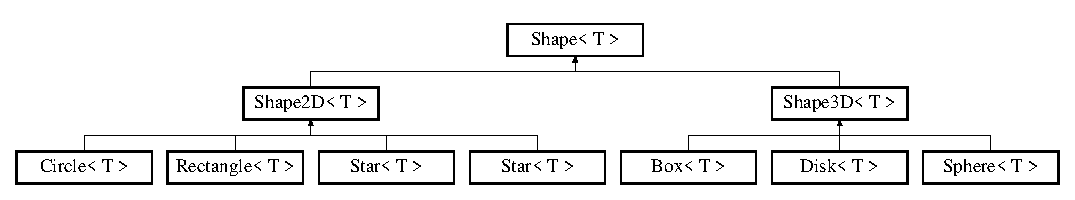
\includegraphics[height=2.242991cm]{classShape}
\end{center}
\end{figure}
\subsection*{Public Member Functions}
\begin{DoxyCompactItemize}
\item 
virtual void \mbox{\hyperlink{classShape_ac5a35fe1b2ecb8fcfc050a31c8969805}{set\+\_\+min\+\_\+number\+\_\+of\+\_\+vertexes}} (unsigned num)
\begin{DoxyCompactList}\small\item\em As the name says, it sets minimal number of vertexes for a given shape. \end{DoxyCompactList}\item 
virtual void \mbox{\hyperlink{classShape_a69dabd50440dba1ac463ad6819cdb506}{set\+\_\+vertex\+\_\+colors}} (\mbox{\hyperlink{type__definitions_8hpp_accb98a876f193a416d9c8a02fe22d526}{aligned\+\_\+vector}}$<$ float $>$ \&colors\+\_\+)
\item 
\mbox{\hyperlink{type__definitions_8hpp_accb98a876f193a416d9c8a02fe22d526}{aligned\+\_\+vector}}$<$ T $>$ \mbox{\hyperlink{classShape_a3729bbdd0c4e4f3379498734807bb545}{get\+\_\+vertexes}} ()
\item 
\mbox{\hyperlink{type__definitions_8hpp_accb98a876f193a416d9c8a02fe22d526}{aligned\+\_\+vector}}$<$ T $>$ \mbox{\hyperlink{classShape_aabe9bd208b0ece9824cb45deccc11ba7}{get\+\_\+colors}} ()
\item 
unsigned \mbox{\hyperlink{classShape_a131e85c7f5cad85bffb92e6719117cab}{num\+\_\+vertexes}} ()
\item 
virtual unsigned \mbox{\hyperlink{classShape_a58713d8cf7c4175e7c76eae75c94bc13}{get\+\_\+vertex\+\_\+size}} ()
\item 
void \mbox{\hyperlink{classShape_aabeb601fe95b412987d5b5c276bf8a7a}{generate\+\_\+random\+\_\+colors}} ()
\begin{DoxyCompactList}\small\item\em Generate random colors for each vertex. \end{DoxyCompactList}\end{DoxyCompactItemize}
\subsection*{Protected Member Functions}
\begin{DoxyCompactItemize}
\item 
void \mbox{\hyperlink{classShape_a8b4f54a694871f9d131fdd105e1ca709}{initialize\+\_\+buffers}} ()
\begin{DoxyCompactList}\small\item\em Allocates and initializes vertex buffer object, element buffer object and vertex array object. It also allocates color buffer -\/ where color for each vertex is stored. \end{DoxyCompactList}\end{DoxyCompactItemize}
\subsection*{Protected Attributes}
\begin{DoxyCompactItemize}
\item 
unsigned \mbox{\hyperlink{classShape_a7cf9cc243cdd64215eca4d81704c7199}{vertex\+\_\+size}} = 0
\item 
\mbox{\hyperlink{type__definitions_8hpp_accb98a876f193a416d9c8a02fe22d526}{aligned\+\_\+vector}}$<$ T $>$ \mbox{\hyperlink{classShape_a50296217cf654fc7b756b67a2f0305c2}{vertexes}}
\item 
char \mbox{\hyperlink{classShape_a851fcb33238286342f670d27443ffdfc}{draw\+\_\+type}}
\item 
\mbox{\hyperlink{type__definitions_8hpp_accb98a876f193a416d9c8a02fe22d526}{aligned\+\_\+vector}}$<$ int $>$ \mbox{\hyperlink{classShape_accef3084e7e3897e01806b90da0a0ec8}{element\+\_\+array}}
\item 
bool \mbox{\hyperlink{classShape_a216866713d16c882a0f0b0b0a89d350d}{colors\+\_\+loaded}}
\item 
unsigned \mbox{\hyperlink{classShape_a5ca89aadcd89bb475d6ca88acf733ce6}{V\+BO}}
\item 
unsigned \mbox{\hyperlink{classShape_a30771567edd66db5d14dc630f2d63f82}{V\+AO}}
\item 
unsigned \mbox{\hyperlink{classShape_a95c775e548b129e23d2dd32e23fb0f3e}{E\+BO}}
\item 
unsigned \mbox{\hyperlink{classShape_a66502f6f87b46a705d131dc7b0b67d42}{C\+BO}}
\item 
unsigned \mbox{\hyperlink{classShape_acb30d3bdd3434dc2cb3074a4d61985ed}{min\+\_\+vertexes}}
\item 
\mbox{\hyperlink{type__definitions_8hpp_accb98a876f193a416d9c8a02fe22d526}{aligned\+\_\+vector}}$<$ float $>$ \mbox{\hyperlink{classShape_a1590ef02d7090f28d1ad312fd46f5030}{vertex\+\_\+colors}}
\end{DoxyCompactItemize}
\subsection*{Friends}
\begin{DoxyCompactItemize}
\item 
void \mbox{\hyperlink{classShape_a0f7d9c8330ae4f062c6f569a7400e1f0}{draw}} (\mbox{\hyperlink{classShape}{Shape}}$<$ T $>$ \&, \mbox{\hyperlink{classShader}{Shader}}$<$ \mbox{\hyperlink{render_8hpp_a24e288e18eb7b6e01de7565001fedb60aa98862073f71a928bad5099cc3e1c2ed}{R\+E\+N\+D\+E\+R\+\_\+\+T\+Y\+P\+E\+::\+U\+N\+I\+F\+O\+R\+M\+\_\+\+C\+O\+L\+OR}} $>$ \&, std\+::array$<$ float, 3 $>$, std\+::array$<$ float, 3 $>$, std\+::array$<$ float, 3 $>$, float, glm\+::vec4)
\item 
void \mbox{\hyperlink{classShape_a29e514c040e0781bfa2e08bcde4a7557}{draw}} (\mbox{\hyperlink{classShape}{Shape}}$<$ T $>$ \&, \mbox{\hyperlink{classShader}{Shader}}$<$ \mbox{\hyperlink{render_8hpp_a24e288e18eb7b6e01de7565001fedb60a9d34355b5a26c54b5dbab1e45245a6f4}{R\+E\+N\+D\+E\+R\+\_\+\+T\+Y\+P\+E\+::\+C\+U\+S\+T\+O\+M\+\_\+\+C\+O\+L\+OR}} $>$ \&, std\+::array$<$ float, 3 $>$, std\+::array$<$ float, 3 $>$, std\+::array$<$ float, 3 $>$, float)
\item 
void \mbox{\hyperlink{classShape_ad57e4dd441b60269c43114f31ffa6085}{draw\+\_\+wireframe}} (\mbox{\hyperlink{classShape}{Shape}}$<$ T $>$ \&shape, \mbox{\hyperlink{classShader}{Shader}}$<$ \mbox{\hyperlink{render_8hpp_a24e288e18eb7b6e01de7565001fedb60aa98862073f71a928bad5099cc3e1c2ed}{R\+E\+N\+D\+E\+R\+\_\+\+T\+Y\+P\+E\+::\+U\+N\+I\+F\+O\+R\+M\+\_\+\+C\+O\+L\+OR}} $>$ \&shader\+\_\+object, std\+::array$<$ float, 3 $>$ scale, std\+::array$<$ float, 3 $>$ position, std\+::array$<$ float, 3 $>$ rotation\+\_\+axis, float angle, glm\+::vec4)
\item 
void \mbox{\hyperlink{classShape_aaff31c90cf40c78284454009c9fe0966}{draw\+\_\+2d\+\_\+object}} (\mbox{\hyperlink{classShape}{Shape}}$<$ T $>$ \&shape, \mbox{\hyperlink{classShader}{Shader}}$<$ \mbox{\hyperlink{render_8hpp_a24e288e18eb7b6e01de7565001fedb60aa98862073f71a928bad5099cc3e1c2ed}{R\+E\+N\+D\+E\+R\+\_\+\+T\+Y\+P\+E\+::\+U\+N\+I\+F\+O\+R\+M\+\_\+\+C\+O\+L\+OR}} $>$ \&shader\+\_\+object, std\+::array$<$ float, 3 $>$ scale, std\+::array$<$ float, 3 $>$ position, std\+::array$<$ float, 3 $>$ rotation\+\_\+axis, float angle, glm\+::vec4)
\end{DoxyCompactItemize}


\subsection{Detailed Description}
\subsubsection*{template$<$typename T$>$\newline
class Shape$<$ T $>$}

virtual base class for 2D and 3D shapes 

All shapes inherit from this class. It contains all basic structures for drawing including opengl buffers. 

\subsection{Member Function Documentation}
\mbox{\Hypertarget{classShape_aabeb601fe95b412987d5b5c276bf8a7a}\label{classShape_aabeb601fe95b412987d5b5c276bf8a7a}} 
\index{Shape@{Shape}!generate\+\_\+random\+\_\+colors@{generate\+\_\+random\+\_\+colors}}
\index{generate\+\_\+random\+\_\+colors@{generate\+\_\+random\+\_\+colors}!Shape@{Shape}}
\subsubsection{\texorpdfstring{generate\+\_\+random\+\_\+colors()}{generate\_random\_colors()}}
{\footnotesize\ttfamily template$<$typename T$>$ \\
void \mbox{\hyperlink{classShape}{Shape}}$<$ T $>$\+::generate\+\_\+random\+\_\+colors (\begin{DoxyParamCaption}{ }\end{DoxyParamCaption})\hspace{0.3cm}{\ttfamily [inline]}}



Generate random colors for each vertex. 

\mbox{\Hypertarget{classShape_aabe9bd208b0ece9824cb45deccc11ba7}\label{classShape_aabe9bd208b0ece9824cb45deccc11ba7}} 
\index{Shape@{Shape}!get\+\_\+colors@{get\+\_\+colors}}
\index{get\+\_\+colors@{get\+\_\+colors}!Shape@{Shape}}
\subsubsection{\texorpdfstring{get\+\_\+colors()}{get\_colors()}}
{\footnotesize\ttfamily template$<$typename T$>$ \\
\mbox{\hyperlink{type__definitions_8hpp_accb98a876f193a416d9c8a02fe22d526}{aligned\+\_\+vector}}$<$T$>$ \mbox{\hyperlink{classShape}{Shape}}$<$ T $>$\+::get\+\_\+colors (\begin{DoxyParamCaption}{ }\end{DoxyParamCaption})\hspace{0.3cm}{\ttfamily [inline]}}

\mbox{\Hypertarget{classShape_a58713d8cf7c4175e7c76eae75c94bc13}\label{classShape_a58713d8cf7c4175e7c76eae75c94bc13}} 
\index{Shape@{Shape}!get\+\_\+vertex\+\_\+size@{get\+\_\+vertex\+\_\+size}}
\index{get\+\_\+vertex\+\_\+size@{get\+\_\+vertex\+\_\+size}!Shape@{Shape}}
\subsubsection{\texorpdfstring{get\+\_\+vertex\+\_\+size()}{get\_vertex\_size()}}
{\footnotesize\ttfamily template$<$typename T$>$ \\
virtual unsigned \mbox{\hyperlink{classShape}{Shape}}$<$ T $>$\+::get\+\_\+vertex\+\_\+size (\begin{DoxyParamCaption}{ }\end{DoxyParamCaption})\hspace{0.3cm}{\ttfamily [inline]}, {\ttfamily [virtual]}}

\mbox{\Hypertarget{classShape_a3729bbdd0c4e4f3379498734807bb545}\label{classShape_a3729bbdd0c4e4f3379498734807bb545}} 
\index{Shape@{Shape}!get\+\_\+vertexes@{get\+\_\+vertexes}}
\index{get\+\_\+vertexes@{get\+\_\+vertexes}!Shape@{Shape}}
\subsubsection{\texorpdfstring{get\+\_\+vertexes()}{get\_vertexes()}}
{\footnotesize\ttfamily template$<$typename T$>$ \\
\mbox{\hyperlink{type__definitions_8hpp_accb98a876f193a416d9c8a02fe22d526}{aligned\+\_\+vector}}$<$T$>$ \mbox{\hyperlink{classShape}{Shape}}$<$ T $>$\+::get\+\_\+vertexes (\begin{DoxyParamCaption}{ }\end{DoxyParamCaption})\hspace{0.3cm}{\ttfamily [inline]}}

\mbox{\Hypertarget{classShape_a8b4f54a694871f9d131fdd105e1ca709}\label{classShape_a8b4f54a694871f9d131fdd105e1ca709}} 
\index{Shape@{Shape}!initialize\+\_\+buffers@{initialize\+\_\+buffers}}
\index{initialize\+\_\+buffers@{initialize\+\_\+buffers}!Shape@{Shape}}
\subsubsection{\texorpdfstring{initialize\+\_\+buffers()}{initialize\_buffers()}}
{\footnotesize\ttfamily template$<$typename T$>$ \\
void \mbox{\hyperlink{classShape}{Shape}}$<$ T $>$\+::initialize\+\_\+buffers (\begin{DoxyParamCaption}{ }\end{DoxyParamCaption})\hspace{0.3cm}{\ttfamily [inline]}, {\ttfamily [protected]}}



Allocates and initializes vertex buffer object, element buffer object and vertex array object. It also allocates color buffer -\/ where color for each vertex is stored. 

\mbox{\Hypertarget{classShape_a131e85c7f5cad85bffb92e6719117cab}\label{classShape_a131e85c7f5cad85bffb92e6719117cab}} 
\index{Shape@{Shape}!num\+\_\+vertexes@{num\+\_\+vertexes}}
\index{num\+\_\+vertexes@{num\+\_\+vertexes}!Shape@{Shape}}
\subsubsection{\texorpdfstring{num\+\_\+vertexes()}{num\_vertexes()}}
{\footnotesize\ttfamily template$<$typename T$>$ \\
unsigned \mbox{\hyperlink{classShape}{Shape}}$<$ T $>$\+::num\+\_\+vertexes (\begin{DoxyParamCaption}{ }\end{DoxyParamCaption})\hspace{0.3cm}{\ttfamily [inline]}}

\mbox{\Hypertarget{classShape_ac5a35fe1b2ecb8fcfc050a31c8969805}\label{classShape_ac5a35fe1b2ecb8fcfc050a31c8969805}} 
\index{Shape@{Shape}!set\+\_\+min\+\_\+number\+\_\+of\+\_\+vertexes@{set\+\_\+min\+\_\+number\+\_\+of\+\_\+vertexes}}
\index{set\+\_\+min\+\_\+number\+\_\+of\+\_\+vertexes@{set\+\_\+min\+\_\+number\+\_\+of\+\_\+vertexes}!Shape@{Shape}}
\subsubsection{\texorpdfstring{set\+\_\+min\+\_\+number\+\_\+of\+\_\+vertexes()}{set\_min\_number\_of\_vertexes()}}
{\footnotesize\ttfamily template$<$typename T$>$ \\
virtual void \mbox{\hyperlink{classShape}{Shape}}$<$ T $>$\+::set\+\_\+min\+\_\+number\+\_\+of\+\_\+vertexes (\begin{DoxyParamCaption}\item[{unsigned}]{num }\end{DoxyParamCaption})\hspace{0.3cm}{\ttfamily [inline]}, {\ttfamily [virtual]}}



As the name says, it sets minimal number of vertexes for a given shape. 


\begin{DoxyParams}{Parameters}
{\em num} & minimal number of vertexes \\
\hline
\end{DoxyParams}
\mbox{\Hypertarget{classShape_a69dabd50440dba1ac463ad6819cdb506}\label{classShape_a69dabd50440dba1ac463ad6819cdb506}} 
\index{Shape@{Shape}!set\+\_\+vertex\+\_\+colors@{set\+\_\+vertex\+\_\+colors}}
\index{set\+\_\+vertex\+\_\+colors@{set\+\_\+vertex\+\_\+colors}!Shape@{Shape}}
\subsubsection{\texorpdfstring{set\+\_\+vertex\+\_\+colors()}{set\_vertex\_colors()}}
{\footnotesize\ttfamily template$<$typename T$>$ \\
virtual void \mbox{\hyperlink{classShape}{Shape}}$<$ T $>$\+::set\+\_\+vertex\+\_\+colors (\begin{DoxyParamCaption}\item[{\mbox{\hyperlink{type__definitions_8hpp_accb98a876f193a416d9c8a02fe22d526}{aligned\+\_\+vector}}$<$ float $>$ \&}]{colors\+\_\+ }\end{DoxyParamCaption})\hspace{0.3cm}{\ttfamily [inline]}, {\ttfamily [virtual]}}



\subsection{Friends And Related Function Documentation}
\mbox{\Hypertarget{classShape_a0f7d9c8330ae4f062c6f569a7400e1f0}\label{classShape_a0f7d9c8330ae4f062c6f569a7400e1f0}} 
\index{Shape@{Shape}!draw@{draw}}
\index{draw@{draw}!Shape@{Shape}}
\subsubsection{\texorpdfstring{draw}{draw}\hspace{0.1cm}{\footnotesize\ttfamily [1/2]}}
{\footnotesize\ttfamily template$<$typename T$>$ \\
void draw (\begin{DoxyParamCaption}\item[{\mbox{\hyperlink{classShape}{Shape}}$<$ T $>$ \&}]{shape,  }\item[{\mbox{\hyperlink{classShader}{Shader}}$<$ \mbox{\hyperlink{render_8hpp_a24e288e18eb7b6e01de7565001fedb60aa98862073f71a928bad5099cc3e1c2ed}{R\+E\+N\+D\+E\+R\+\_\+\+T\+Y\+P\+E\+::\+U\+N\+I\+F\+O\+R\+M\+\_\+\+C\+O\+L\+OR}} $>$ \&}]{shader\+\_\+object,  }\item[{std\+::array$<$ float, 3 $>$}]{scale = {\ttfamily \{0.5,~0.5,~0.5\}},  }\item[{std\+::array$<$ float, 3 $>$}]{position = {\ttfamily \{0,~0,~1\}},  }\item[{std\+::array$<$ float, 3 $>$}]{rotation\+\_\+axis = {\ttfamily \{0,~0,~1\}},  }\item[{float}]{angle = {\ttfamily 0},  }\item[{glm\+::vec4}]{color = {\ttfamily \{0.5,~0.5,~0.5,~0.5\}} }\end{DoxyParamCaption})\hspace{0.3cm}{\ttfamily [friend]}}

\mbox{\Hypertarget{classShape_a29e514c040e0781bfa2e08bcde4a7557}\label{classShape_a29e514c040e0781bfa2e08bcde4a7557}} 
\index{Shape@{Shape}!draw@{draw}}
\index{draw@{draw}!Shape@{Shape}}
\subsubsection{\texorpdfstring{draw}{draw}\hspace{0.1cm}{\footnotesize\ttfamily [2/2]}}
{\footnotesize\ttfamily template$<$typename T$>$ \\
void draw (\begin{DoxyParamCaption}\item[{\mbox{\hyperlink{classShape}{Shape}}$<$ T $>$ \&}]{shape,  }\item[{\mbox{\hyperlink{classShader}{Shader}}$<$ \mbox{\hyperlink{render_8hpp_a24e288e18eb7b6e01de7565001fedb60a9d34355b5a26c54b5dbab1e45245a6f4}{R\+E\+N\+D\+E\+R\+\_\+\+T\+Y\+P\+E\+::\+C\+U\+S\+T\+O\+M\+\_\+\+C\+O\+L\+OR}} $>$ \&}]{shader\+\_\+object,  }\item[{std\+::array$<$ float, 3 $>$}]{scale = {\ttfamily \{0.5,~0.5,~0.5\}},  }\item[{std\+::array$<$ float, 3 $>$}]{position = {\ttfamily \{0,~0,~1\}},  }\item[{std\+::array$<$ float, 3 $>$}]{rotation\+\_\+axis = {\ttfamily \{0,~0,~1\}},  }\item[{float}]{angle = {\ttfamily 0} }\end{DoxyParamCaption})\hspace{0.3cm}{\ttfamily [friend]}}

\mbox{\Hypertarget{classShape_aaff31c90cf40c78284454009c9fe0966}\label{classShape_aaff31c90cf40c78284454009c9fe0966}} 
\index{Shape@{Shape}!draw\+\_\+2d\+\_\+object@{draw\+\_\+2d\+\_\+object}}
\index{draw\+\_\+2d\+\_\+object@{draw\+\_\+2d\+\_\+object}!Shape@{Shape}}
\subsubsection{\texorpdfstring{draw\+\_\+2d\+\_\+object}{draw\_2d\_object}}
{\footnotesize\ttfamily template$<$typename T$>$ \\
void draw\+\_\+2d\+\_\+object (\begin{DoxyParamCaption}\item[{\mbox{\hyperlink{classShape}{Shape}}$<$ T $>$ \&}]{shape,  }\item[{\mbox{\hyperlink{classShader}{Shader}}$<$ \mbox{\hyperlink{render_8hpp_a24e288e18eb7b6e01de7565001fedb60aa98862073f71a928bad5099cc3e1c2ed}{R\+E\+N\+D\+E\+R\+\_\+\+T\+Y\+P\+E\+::\+U\+N\+I\+F\+O\+R\+M\+\_\+\+C\+O\+L\+OR}} $>$ \&}]{shader\+\_\+object,  }\item[{std\+::array$<$ float, 3 $>$}]{scale = {\ttfamily \{0.5,~0.5,~0.5\}},  }\item[{std\+::array$<$ float, 3 $>$}]{position = {\ttfamily \{0,~0,~1\}},  }\item[{std\+::array$<$ float, 3 $>$}]{rotation\+\_\+axis = {\ttfamily \{0,~0,~1\}},  }\item[{float}]{angle = {\ttfamily 0},  }\item[{glm\+::vec4}]{color = {\ttfamily \{0.5,~0.5,~0.5,~0.5\}} }\end{DoxyParamCaption})\hspace{0.3cm}{\ttfamily [friend]}}

\mbox{\Hypertarget{classShape_ad57e4dd441b60269c43114f31ffa6085}\label{classShape_ad57e4dd441b60269c43114f31ffa6085}} 
\index{Shape@{Shape}!draw\+\_\+wireframe@{draw\+\_\+wireframe}}
\index{draw\+\_\+wireframe@{draw\+\_\+wireframe}!Shape@{Shape}}
\subsubsection{\texorpdfstring{draw\+\_\+wireframe}{draw\_wireframe}}
{\footnotesize\ttfamily template$<$typename T$>$ \\
void draw\+\_\+wireframe (\begin{DoxyParamCaption}\item[{\mbox{\hyperlink{classShape}{Shape}}$<$ T $>$ \&}]{shape,  }\item[{\mbox{\hyperlink{classShader}{Shader}}$<$ \mbox{\hyperlink{render_8hpp_a24e288e18eb7b6e01de7565001fedb60aa98862073f71a928bad5099cc3e1c2ed}{R\+E\+N\+D\+E\+R\+\_\+\+T\+Y\+P\+E\+::\+U\+N\+I\+F\+O\+R\+M\+\_\+\+C\+O\+L\+OR}} $>$ \&}]{shader\+\_\+object,  }\item[{std\+::array$<$ float, 3 $>$}]{scale = {\ttfamily \{0.5,~0.5,~0.5\}},  }\item[{std\+::array$<$ float, 3 $>$}]{position = {\ttfamily \{0,~0,~1\}},  }\item[{std\+::array$<$ float, 3 $>$}]{rotation\+\_\+axis = {\ttfamily \{0,~0,~1\}},  }\item[{float}]{angle = {\ttfamily 0},  }\item[{glm\+::vec4}]{color = {\ttfamily \{0.5,~0.5,~0.5,~0.5\}} }\end{DoxyParamCaption})\hspace{0.3cm}{\ttfamily [friend]}}



\subsection{Member Data Documentation}
\mbox{\Hypertarget{classShape_a66502f6f87b46a705d131dc7b0b67d42}\label{classShape_a66502f6f87b46a705d131dc7b0b67d42}} 
\index{Shape@{Shape}!C\+BO@{C\+BO}}
\index{C\+BO@{C\+BO}!Shape@{Shape}}
\subsubsection{\texorpdfstring{C\+BO}{CBO}}
{\footnotesize\ttfamily template$<$typename T$>$ \\
unsigned \mbox{\hyperlink{classShape}{Shape}}$<$ T $>$\+::C\+BO\hspace{0.3cm}{\ttfamily [protected]}}

color buffer address \mbox{\Hypertarget{classShape_a216866713d16c882a0f0b0b0a89d350d}\label{classShape_a216866713d16c882a0f0b0b0a89d350d}} 
\index{Shape@{Shape}!colors\+\_\+loaded@{colors\+\_\+loaded}}
\index{colors\+\_\+loaded@{colors\+\_\+loaded}!Shape@{Shape}}
\subsubsection{\texorpdfstring{colors\+\_\+loaded}{colors\_loaded}}
{\footnotesize\ttfamily template$<$typename T$>$ \\
bool \mbox{\hyperlink{classShape}{Shape}}$<$ T $>$\+::colors\+\_\+loaded\hspace{0.3cm}{\ttfamily [protected]}}

{\bfseries Initial value\+:}
\begin{DoxyCode}
=
        \textcolor{keyword}{false}
\end{DoxyCode}
indicator whether color have been loaded or not vertex size can consist of 2, 3 or 4 points; this is important for correct interpretation of vertexes vector \mbox{\Hypertarget{classShape_a851fcb33238286342f670d27443ffdfc}\label{classShape_a851fcb33238286342f670d27443ffdfc}} 
\index{Shape@{Shape}!draw\+\_\+type@{draw\+\_\+type}}
\index{draw\+\_\+type@{draw\+\_\+type}!Shape@{Shape}}
\subsubsection{\texorpdfstring{draw\+\_\+type}{draw\_type}}
{\footnotesize\ttfamily template$<$typename T$>$ \\
char \mbox{\hyperlink{classShape}{Shape}}$<$ T $>$\+::draw\+\_\+type\hspace{0.3cm}{\ttfamily [protected]}}

this can either be \textquotesingle{}E\textquotesingle{} or \textquotesingle{}V\textquotesingle{}, depending on wheather to draw elements (element buffer) or vertexes (vertex buffer object) \mbox{\Hypertarget{classShape_a95c775e548b129e23d2dd32e23fb0f3e}\label{classShape_a95c775e548b129e23d2dd32e23fb0f3e}} 
\index{Shape@{Shape}!E\+BO@{E\+BO}}
\index{E\+BO@{E\+BO}!Shape@{Shape}}
\subsubsection{\texorpdfstring{E\+BO}{EBO}}
{\footnotesize\ttfamily template$<$typename T$>$ \\
unsigned \mbox{\hyperlink{classShape}{Shape}}$<$ T $>$\+::E\+BO\hspace{0.3cm}{\ttfamily [protected]}}

element buffer address \mbox{\Hypertarget{classShape_accef3084e7e3897e01806b90da0a0ec8}\label{classShape_accef3084e7e3897e01806b90da0a0ec8}} 
\index{Shape@{Shape}!element\+\_\+array@{element\+\_\+array}}
\index{element\+\_\+array@{element\+\_\+array}!Shape@{Shape}}
\subsubsection{\texorpdfstring{element\+\_\+array}{element\_array}}
{\footnotesize\ttfamily template$<$typename T$>$ \\
\mbox{\hyperlink{type__definitions_8hpp_accb98a876f193a416d9c8a02fe22d526}{aligned\+\_\+vector}}$<$int$>$ \mbox{\hyperlink{classShape}{Shape}}$<$ T $>$\+::element\+\_\+array\hspace{0.3cm}{\ttfamily [protected]}}

vector holding all elements in correct order \mbox{\Hypertarget{classShape_acb30d3bdd3434dc2cb3074a4d61985ed}\label{classShape_acb30d3bdd3434dc2cb3074a4d61985ed}} 
\index{Shape@{Shape}!min\+\_\+vertexes@{min\+\_\+vertexes}}
\index{min\+\_\+vertexes@{min\+\_\+vertexes}!Shape@{Shape}}
\subsubsection{\texorpdfstring{min\+\_\+vertexes}{min\_vertexes}}
{\footnotesize\ttfamily template$<$typename T$>$ \\
unsigned \mbox{\hyperlink{classShape}{Shape}}$<$ T $>$\+::min\+\_\+vertexes\hspace{0.3cm}{\ttfamily [protected]}}

{\bfseries Initial value\+:}
\begin{DoxyCode}
=
        5
\end{DoxyCode}
minimal number of vertexes to be generated for a given shape \mbox{\Hypertarget{classShape_a30771567edd66db5d14dc630f2d63f82}\label{classShape_a30771567edd66db5d14dc630f2d63f82}} 
\index{Shape@{Shape}!V\+AO@{V\+AO}}
\index{V\+AO@{V\+AO}!Shape@{Shape}}
\subsubsection{\texorpdfstring{V\+AO}{VAO}}
{\footnotesize\ttfamily template$<$typename T$>$ \\
unsigned \mbox{\hyperlink{classShape}{Shape}}$<$ T $>$\+::V\+AO\hspace{0.3cm}{\ttfamily [protected]}}

vertex array object \mbox{\Hypertarget{classShape_a5ca89aadcd89bb475d6ca88acf733ce6}\label{classShape_a5ca89aadcd89bb475d6ca88acf733ce6}} 
\index{Shape@{Shape}!V\+BO@{V\+BO}}
\index{V\+BO@{V\+BO}!Shape@{Shape}}
\subsubsection{\texorpdfstring{V\+BO}{VBO}}
{\footnotesize\ttfamily template$<$typename T$>$ \\
unsigned \mbox{\hyperlink{classShape}{Shape}}$<$ T $>$\+::V\+BO\hspace{0.3cm}{\ttfamily [protected]}}

vertex buffer object \mbox{\Hypertarget{classShape_a1590ef02d7090f28d1ad312fd46f5030}\label{classShape_a1590ef02d7090f28d1ad312fd46f5030}} 
\index{Shape@{Shape}!vertex\+\_\+colors@{vertex\+\_\+colors}}
\index{vertex\+\_\+colors@{vertex\+\_\+colors}!Shape@{Shape}}
\subsubsection{\texorpdfstring{vertex\+\_\+colors}{vertex\_colors}}
{\footnotesize\ttfamily template$<$typename T$>$ \\
\mbox{\hyperlink{type__definitions_8hpp_accb98a876f193a416d9c8a02fe22d526}{aligned\+\_\+vector}}$<$float$>$ \mbox{\hyperlink{classShape}{Shape}}$<$ T $>$\+::vertex\+\_\+colors\hspace{0.3cm}{\ttfamily [protected]}}

Vector holding a color for each vertex. Four consequtive numbers form a rgb color value \mbox{\Hypertarget{classShape_a7cf9cc243cdd64215eca4d81704c7199}\label{classShape_a7cf9cc243cdd64215eca4d81704c7199}} 
\index{Shape@{Shape}!vertex\+\_\+size@{vertex\+\_\+size}}
\index{vertex\+\_\+size@{vertex\+\_\+size}!Shape@{Shape}}
\subsubsection{\texorpdfstring{vertex\+\_\+size}{vertex\_size}}
{\footnotesize\ttfamily template$<$typename T$>$ \\
unsigned \mbox{\hyperlink{classShape}{Shape}}$<$ T $>$\+::vertex\+\_\+size = 0\hspace{0.3cm}{\ttfamily [protected]}}

\mbox{\Hypertarget{classShape_a50296217cf654fc7b756b67a2f0305c2}\label{classShape_a50296217cf654fc7b756b67a2f0305c2}} 
\index{Shape@{Shape}!vertexes@{vertexes}}
\index{vertexes@{vertexes}!Shape@{Shape}}
\subsubsection{\texorpdfstring{vertexes}{vertexes}}
{\footnotesize\ttfamily template$<$typename T$>$ \\
\mbox{\hyperlink{type__definitions_8hpp_accb98a876f193a416d9c8a02fe22d526}{aligned\+\_\+vector}}$<$T$>$ \mbox{\hyperlink{classShape}{Shape}}$<$ T $>$\+::vertexes\hspace{0.3cm}{\ttfamily [protected]}}

Vector holding all vertexes; 2,3 or 4 consequtive numbers form a vertex 

The documentation for this class was generated from the following files\+:\begin{DoxyCompactItemize}
\item 
src/\mbox{\hyperlink{drawing__functions_8hpp}{drawing\+\_\+functions.\+hpp}}\item 
src/\mbox{\hyperlink{shape_8hpp}{shape.\+hpp}}\end{DoxyCompactItemize}

\hypertarget{classShape2D}{}\section{Shape2D$<$ T $>$ Class Template Reference}
\label{classShape2D}\index{Shape2\+D$<$ T $>$@{Shape2\+D$<$ T $>$}}


\mbox{\hyperlink{classThis}{This}} is a base class for all 2D shapes.  




{\ttfamily \#include \char`\"{}drawing\+\_\+functions.\+hpp\char`\"{}}

Inheritance diagram for Shape2D$<$ T $>$\+:\begin{figure}[H]
\begin{center}
\leavevmode
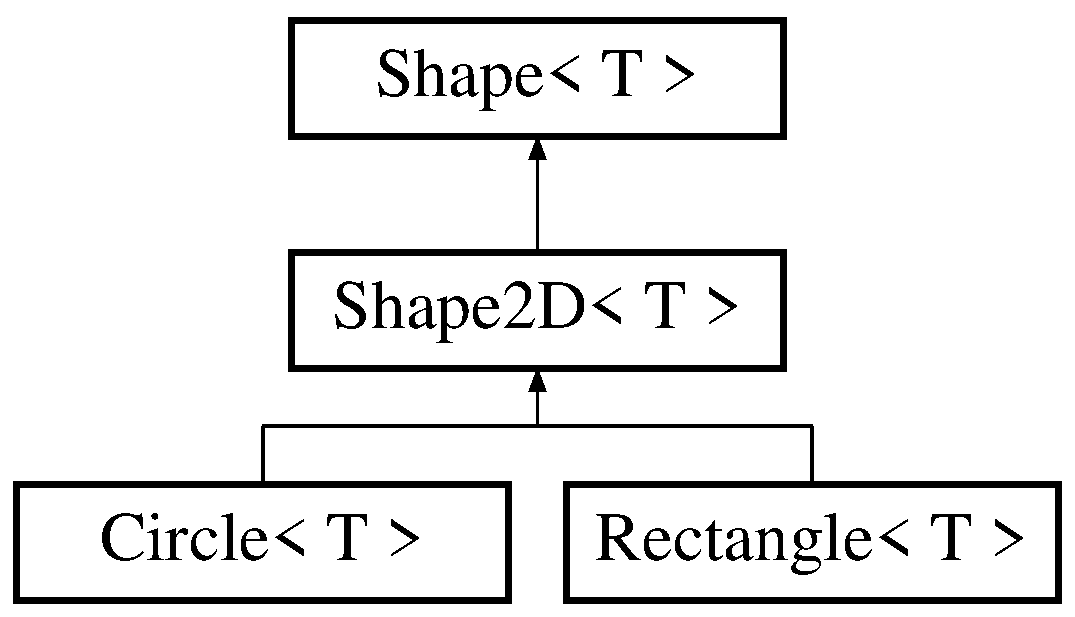
\includegraphics[height=2.688000cm]{classShape2D}
\end{center}
\end{figure}
\subsection*{Public Member Functions}
\begin{DoxyCompactItemize}
\item 
\mbox{\hyperlink{type__definitions_8hpp_a087efd587d66b881646ef378f1919c90}{aligned\+\_\+vector}}$<$ T $>$ \mbox{\hyperlink{classShape2D_af67c7aed6e58b5aa0e3518a3ad1de75b}{get\+\_\+filling\+\_\+vertexes}} ()
\end{DoxyCompactItemize}
\subsection*{Protected Member Functions}
\begin{DoxyCompactItemize}
\item 
virtual \mbox{\hyperlink{glad_8h_a950fc91edb4504f62f1c577bf4727c29}{void}} \mbox{\hyperlink{classShape2D_a917c3277ca262ec557930c8cc837c204}{generate\+\_\+filling\+\_\+vbo}} ()
\item 
{\footnotesize template$<$$>$ }\\\mbox{\hyperlink{glad_8h_a950fc91edb4504f62f1c577bf4727c29}{void}} \mbox{\hyperlink{classShape2D_a328d401b8f1962078e904d4b1003d7a5}{generate\+\_\+filling\+\_\+vbo}} ()
\begin{DoxyCompactList}\small\item\em Generates vertexes which fill the interior of 2D shapes. \end{DoxyCompactList}\end{DoxyCompactItemize}
\subsection*{Protected Attributes}
\begin{DoxyCompactItemize}
\item 
unsigned \mbox{\hyperlink{classShape2D_a220cf4cf96da8bd43627ffffd00a0718}{F\+I\+L\+L\+I\+N\+G\+\_\+\+V\+BO}}
\item 
unsigned \mbox{\hyperlink{classShape2D_affa1082cd6e91cce5af4cb10c1b3435f}{F\+I\+L\+L\+I\+N\+G\+\_\+\+E\+BO}}
\item 
char \mbox{\hyperlink{classShape2D_ab24ceddaa0114eda3ae699f8fb3503ca}{filling\+\_\+draw\+\_\+type}}
\item 
\mbox{\hyperlink{type__definitions_8hpp_a087efd587d66b881646ef378f1919c90}{aligned\+\_\+vector}}$<$ T $>$ \mbox{\hyperlink{classShape2D_ae3e216c9d8422b47f46bff9259bd17be}{filling\+\_\+vertexes}}
\item 
\mbox{\hyperlink{type__definitions_8hpp_a087efd587d66b881646ef378f1919c90}{aligned\+\_\+vector}}$<$ int $>$ \mbox{\hyperlink{classShape2D_a28d0d6018cb6b73637050d9f3fb1f006}{filling\+\_\+elements}}
\end{DoxyCompactItemize}
\subsection*{Friends}
\begin{DoxyCompactItemize}
\item 
\mbox{\hyperlink{glad_8h_a950fc91edb4504f62f1c577bf4727c29}{void}} \mbox{\hyperlink{classShape2D_a75ed525e537ded17d42e3adad87bd701}{draw\+\_\+2d\+\_\+object}} (\mbox{\hyperlink{classShape2D}{Shape2D}}$<$ T $>$ \&shape, \mbox{\hyperlink{classShader}{Shader}}$<$ \mbox{\hyperlink{shader__class_8hpp_a24e288e18eb7b6e01de7565001fedb60aa98862073f71a928bad5099cc3e1c2ed}{R\+E\+N\+D\+E\+R\+\_\+\+T\+Y\+P\+E\+::\+U\+N\+I\+F\+O\+R\+M\+\_\+\+C\+O\+L\+OR}} $>$ \&shader\+\_\+object, std\+::array$<$ float, 3 $>$ scale, std\+::array$<$ float, 3 $>$ position, std\+::array$<$ float, 3 $>$ rotation\+\_\+axis, float angle, glm\+::vec4)
\begin{DoxyCompactList}\small\item\em draw 2d shape filling of uniform color. \end{DoxyCompactList}\end{DoxyCompactItemize}


\subsection{Detailed Description}
\subsubsection*{template$<$typename T$>$\newline
class Shape2\+D$<$ T $>$}

\mbox{\hyperlink{classThis}{This}} is a base class for all 2D shapes. 

It inherits from \mbox{\hyperlink{classShape}{Shape}} class. Template parameter can either be float of double. It is meant to contain functions common to all 2D shapes. 

\subsection{Member Function Documentation}
\mbox{\Hypertarget{classShape2D_a917c3277ca262ec557930c8cc837c204}\label{classShape2D_a917c3277ca262ec557930c8cc837c204}} 
\index{Shape2D@{Shape2D}!generate\+\_\+filling\+\_\+vbo@{generate\+\_\+filling\+\_\+vbo}}
\index{generate\+\_\+filling\+\_\+vbo@{generate\+\_\+filling\+\_\+vbo}!Shape2D@{Shape2D}}
\subsubsection{\texorpdfstring{generate\+\_\+filling\+\_\+vbo()}{generate\_filling\_vbo()}\hspace{0.1cm}{\footnotesize\ttfamily [1/2]}}
{\footnotesize\ttfamily template$<$typename T$>$ \\
virtual \mbox{\hyperlink{glad_8h_a950fc91edb4504f62f1c577bf4727c29}{void}} \mbox{\hyperlink{classShape2D}{Shape2D}}$<$ T $>$\+::generate\+\_\+filling\+\_\+vbo (\begin{DoxyParamCaption}{ }\end{DoxyParamCaption})\hspace{0.3cm}{\ttfamily [protected]}, {\ttfamily [virtual]}}

\mbox{\Hypertarget{classShape2D_a328d401b8f1962078e904d4b1003d7a5}\label{classShape2D_a328d401b8f1962078e904d4b1003d7a5}} 
\index{Shape2D@{Shape2D}!generate\+\_\+filling\+\_\+vbo@{generate\+\_\+filling\+\_\+vbo}}
\index{generate\+\_\+filling\+\_\+vbo@{generate\+\_\+filling\+\_\+vbo}!Shape2D@{Shape2D}}
\subsubsection{\texorpdfstring{generate\+\_\+filling\+\_\+vbo()}{generate\_filling\_vbo()}\hspace{0.1cm}{\footnotesize\ttfamily [2/2]}}
{\footnotesize\ttfamily template$<$$>$ \\
\mbox{\hyperlink{glad_8h_a950fc91edb4504f62f1c577bf4727c29}{void}} \mbox{\hyperlink{classShape2D}{Shape2D}}$<$ float $>$\+::generate\+\_\+filling\+\_\+vbo (\begin{DoxyParamCaption}{ }\end{DoxyParamCaption})\hspace{0.3cm}{\ttfamily [inline]}, {\ttfamily [protected]}}



Generates vertexes which fill the interior of 2D shapes. 

\mbox{\Hypertarget{classShape2D_af67c7aed6e58b5aa0e3518a3ad1de75b}\label{classShape2D_af67c7aed6e58b5aa0e3518a3ad1de75b}} 
\index{Shape2D@{Shape2D}!get\+\_\+filling\+\_\+vertexes@{get\+\_\+filling\+\_\+vertexes}}
\index{get\+\_\+filling\+\_\+vertexes@{get\+\_\+filling\+\_\+vertexes}!Shape2D@{Shape2D}}
\subsubsection{\texorpdfstring{get\+\_\+filling\+\_\+vertexes()}{get\_filling\_vertexes()}}
{\footnotesize\ttfamily template$<$typename T$>$ \\
\mbox{\hyperlink{type__definitions_8hpp_a087efd587d66b881646ef378f1919c90}{aligned\+\_\+vector}}$<$T$>$ \mbox{\hyperlink{classShape2D}{Shape2D}}$<$ T $>$\+::get\+\_\+filling\+\_\+vertexes (\begin{DoxyParamCaption}{ }\end{DoxyParamCaption})\hspace{0.3cm}{\ttfamily [inline]}}



\subsection{Friends And Related Function Documentation}
\mbox{\Hypertarget{classShape2D_a75ed525e537ded17d42e3adad87bd701}\label{classShape2D_a75ed525e537ded17d42e3adad87bd701}} 
\index{Shape2D@{Shape2D}!draw\+\_\+2d\+\_\+object@{draw\+\_\+2d\+\_\+object}}
\index{draw\+\_\+2d\+\_\+object@{draw\+\_\+2d\+\_\+object}!Shape2D@{Shape2D}}
\subsubsection{\texorpdfstring{draw\+\_\+2d\+\_\+object}{draw\_2d\_object}}
{\footnotesize\ttfamily template$<$typename T$>$ \\
\mbox{\hyperlink{glad_8h_a950fc91edb4504f62f1c577bf4727c29}{void}} draw\+\_\+2d\+\_\+object (\begin{DoxyParamCaption}\item[{\mbox{\hyperlink{classShape2D}{Shape2D}}$<$ T $>$ \&}]{shape,  }\item[{\mbox{\hyperlink{classShader}{Shader}}$<$ \mbox{\hyperlink{shader__class_8hpp_a24e288e18eb7b6e01de7565001fedb60aa98862073f71a928bad5099cc3e1c2ed}{R\+E\+N\+D\+E\+R\+\_\+\+T\+Y\+P\+E\+::\+U\+N\+I\+F\+O\+R\+M\+\_\+\+C\+O\+L\+OR}} $>$ \&}]{shader\+\_\+object,  }\item[{std\+::array$<$ float, 3 $>$}]{scale = {\ttfamily \{0.5,~0.5,~0.5\}},  }\item[{std\+::array$<$ float, 3 $>$}]{position = {\ttfamily \{0,~0,~1\}},  }\item[{std\+::array$<$ float, 3 $>$}]{rotation\+\_\+axis = {\ttfamily \{0,~0,~1\}},  }\item[{float}]{angle = {\ttfamily 0},  }\item[{glm\+::vec4}]{color = {\ttfamily \{0.5,~0.5,~0.5,~0.5\}} }\end{DoxyParamCaption})\hspace{0.3cm}{\ttfamily [friend]}}



draw 2d shape filling of uniform color. 


\begin{DoxyParams}{Parameters}
{\em shape} & An object of type class \mbox{\hyperlink{classShape}{Shape}} to be drawn \\
\hline
{\em shader\+\_\+object} & Object of type class Shader$<$\+R\+E\+N\+D\+E\+R\+\_\+\+T\+Y\+P\+E\+::\+U\+N\+I\+F\+O\+R\+M\+\_\+\+C\+O\+L\+O\+R$>$, which contains correct shader. \\
\hline
{\em scale} & sscales object in x,y and z directions. \\
\hline
{\em position} & translate center of the object to coordinates specified by this vector. \\
\hline
{\em rotation\+\_\+axis} & axis around which object should be rotated. \\
\hline
{\em angle} & Angle specifying how much to rotate the object. \\
\hline
{\em color} & color of the shape -\/ the same for all vertexes \\
\hline
\end{DoxyParams}


\subsection{Member Data Documentation}
\mbox{\Hypertarget{classShape2D_ab24ceddaa0114eda3ae699f8fb3503ca}\label{classShape2D_ab24ceddaa0114eda3ae699f8fb3503ca}} 
\index{Shape2D@{Shape2D}!filling\+\_\+draw\+\_\+type@{filling\+\_\+draw\+\_\+type}}
\index{filling\+\_\+draw\+\_\+type@{filling\+\_\+draw\+\_\+type}!Shape2D@{Shape2D}}
\subsubsection{\texorpdfstring{filling\+\_\+draw\+\_\+type}{filling\_draw\_type}}
{\footnotesize\ttfamily template$<$typename T$>$ \\
char \mbox{\hyperlink{classShape2D}{Shape2D}}$<$ T $>$\+::filling\+\_\+draw\+\_\+type\hspace{0.3cm}{\ttfamily [protected]}}

tells whether to render element buffer -\/ \textquotesingle{}E\textquotesingle{} of array buffer -\/ \textquotesingle{}V\textquotesingle{} \mbox{\Hypertarget{classShape2D_affa1082cd6e91cce5af4cb10c1b3435f}\label{classShape2D_affa1082cd6e91cce5af4cb10c1b3435f}} 
\index{Shape2D@{Shape2D}!F\+I\+L\+L\+I\+N\+G\+\_\+\+E\+BO@{F\+I\+L\+L\+I\+N\+G\+\_\+\+E\+BO}}
\index{F\+I\+L\+L\+I\+N\+G\+\_\+\+E\+BO@{F\+I\+L\+L\+I\+N\+G\+\_\+\+E\+BO}!Shape2D@{Shape2D}}
\subsubsection{\texorpdfstring{F\+I\+L\+L\+I\+N\+G\+\_\+\+E\+BO}{FILLING\_EBO}}
{\footnotesize\ttfamily template$<$typename T$>$ \\
unsigned \mbox{\hyperlink{classShape2D}{Shape2D}}$<$ T $>$\+::F\+I\+L\+L\+I\+N\+G\+\_\+\+E\+BO\hspace{0.3cm}{\ttfamily [protected]}}

2D shapes consist of lines, this buffer contains elements to fill 2D shapes. \mbox{\Hypertarget{classShape2D_a28d0d6018cb6b73637050d9f3fb1f006}\label{classShape2D_a28d0d6018cb6b73637050d9f3fb1f006}} 
\index{Shape2D@{Shape2D}!filling\+\_\+elements@{filling\+\_\+elements}}
\index{filling\+\_\+elements@{filling\+\_\+elements}!Shape2D@{Shape2D}}
\subsubsection{\texorpdfstring{filling\+\_\+elements}{filling\_elements}}
{\footnotesize\ttfamily template$<$typename T$>$ \\
\mbox{\hyperlink{type__definitions_8hpp_a087efd587d66b881646ef378f1919c90}{aligned\+\_\+vector}}$<$int$>$ \mbox{\hyperlink{classShape2D}{Shape2D}}$<$ T $>$\+::filling\+\_\+elements\hspace{0.3cm}{\ttfamily [protected]}}

vertexes for interior of 2D shapes. \mbox{\Hypertarget{classShape2D_a220cf4cf96da8bd43627ffffd00a0718}\label{classShape2D_a220cf4cf96da8bd43627ffffd00a0718}} 
\index{Shape2D@{Shape2D}!F\+I\+L\+L\+I\+N\+G\+\_\+\+V\+BO@{F\+I\+L\+L\+I\+N\+G\+\_\+\+V\+BO}}
\index{F\+I\+L\+L\+I\+N\+G\+\_\+\+V\+BO@{F\+I\+L\+L\+I\+N\+G\+\_\+\+V\+BO}!Shape2D@{Shape2D}}
\subsubsection{\texorpdfstring{F\+I\+L\+L\+I\+N\+G\+\_\+\+V\+BO}{FILLING\_VBO}}
{\footnotesize\ttfamily template$<$typename T$>$ \\
unsigned \mbox{\hyperlink{classShape2D}{Shape2D}}$<$ T $>$\+::F\+I\+L\+L\+I\+N\+G\+\_\+\+V\+BO\hspace{0.3cm}{\ttfamily [protected]}}

2D shapes consist of lines, this buffer is meant to fill 2D shapes. \mbox{\Hypertarget{classShape2D_ae3e216c9d8422b47f46bff9259bd17be}\label{classShape2D_ae3e216c9d8422b47f46bff9259bd17be}} 
\index{Shape2D@{Shape2D}!filling\+\_\+vertexes@{filling\+\_\+vertexes}}
\index{filling\+\_\+vertexes@{filling\+\_\+vertexes}!Shape2D@{Shape2D}}
\subsubsection{\texorpdfstring{filling\+\_\+vertexes}{filling\_vertexes}}
{\footnotesize\ttfamily template$<$typename T$>$ \\
\mbox{\hyperlink{type__definitions_8hpp_a087efd587d66b881646ef378f1919c90}{aligned\+\_\+vector}}$<$T$>$ \mbox{\hyperlink{classShape2D}{Shape2D}}$<$ T $>$\+::filling\+\_\+vertexes\hspace{0.3cm}{\ttfamily [protected]}}

vertexes for interior of 2D shapes. 

The documentation for this class was generated from the following files\+:\begin{DoxyCompactItemize}
\item 
src/display\+\_\+and\+\_\+drawing\+\_\+functions/\mbox{\hyperlink{drawing__functions_8hpp}{drawing\+\_\+functions.\+hpp}}\item 
src/shapes/\mbox{\hyperlink{shape_8hpp}{shape.\+hpp}}\end{DoxyCompactItemize}

\hypertarget{classShape3D}{}\section{Shape3D$<$ T $>$ Class Template Reference}
\label{classShape3D}\index{Shape3\+D$<$ T $>$@{Shape3\+D$<$ T $>$}}


{\ttfamily \#include \char`\"{}shape.\+hpp\char`\"{}}

Inheritance diagram for Shape3D$<$ T $>$\+:\begin{figure}[H]
\begin{center}
\leavevmode
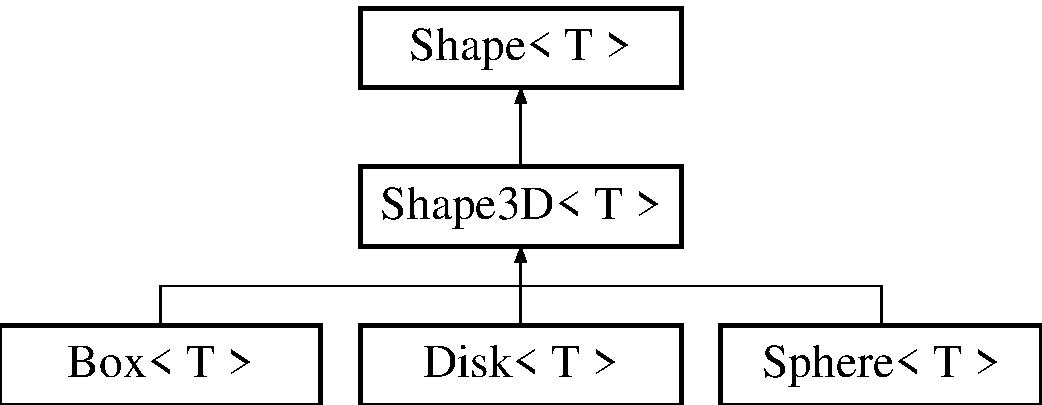
\includegraphics[height=3.000000cm]{classShape3D}
\end{center}
\end{figure}
\subsection*{Public Member Functions}
\begin{DoxyCompactItemize}
\item 
{\footnotesize template$<$typename Q  = T$>$ }\\std\+::enable\+\_\+if$<$ std\+::is\+\_\+same$<$ Q, float $>$\+::value, Q $>$\+::type \mbox{\hyperlink{classShape3D_a2e50becd374a83f43617328dbcc2de3b}{area}} ()
\end{DoxyCompactItemize}
\subsection*{Additional Inherited Members}


\subsection{Member Function Documentation}
\mbox{\Hypertarget{classShape3D_a2e50becd374a83f43617328dbcc2de3b}\label{classShape3D_a2e50becd374a83f43617328dbcc2de3b}} 
\index{Shape3D@{Shape3D}!area@{area}}
\index{area@{area}!Shape3D@{Shape3D}}
\subsubsection{\texorpdfstring{area()}{area()}}
{\footnotesize\ttfamily template$<$typename T $>$ \\
template$<$typename Q  = T$>$ \\
std\+::enable\+\_\+if$<$std\+::is\+\_\+same$<$Q, float$>$\+::value, Q$>$\+::type \mbox{\hyperlink{classShape3D}{Shape3D}}$<$ T $>$\+::area (\begin{DoxyParamCaption}{ }\end{DoxyParamCaption})\hspace{0.3cm}{\ttfamily [inline]}}



The documentation for this class was generated from the following file\+:\begin{DoxyCompactItemize}
\item 
src/\mbox{\hyperlink{shape_8hpp}{shape.\+hpp}}\end{DoxyCompactItemize}

\hypertarget{classSphere}{}\section{Sphere$<$ T $>$ Class Template Reference}
\label{classSphere}\index{Sphere$<$ T $>$@{Sphere$<$ T $>$}}


{\ttfamily \#include \char`\"{}sphere.\+hpp\char`\"{}}

Inheritance diagram for Sphere$<$ T $>$\+:\begin{figure}[H]
\begin{center}
\leavevmode
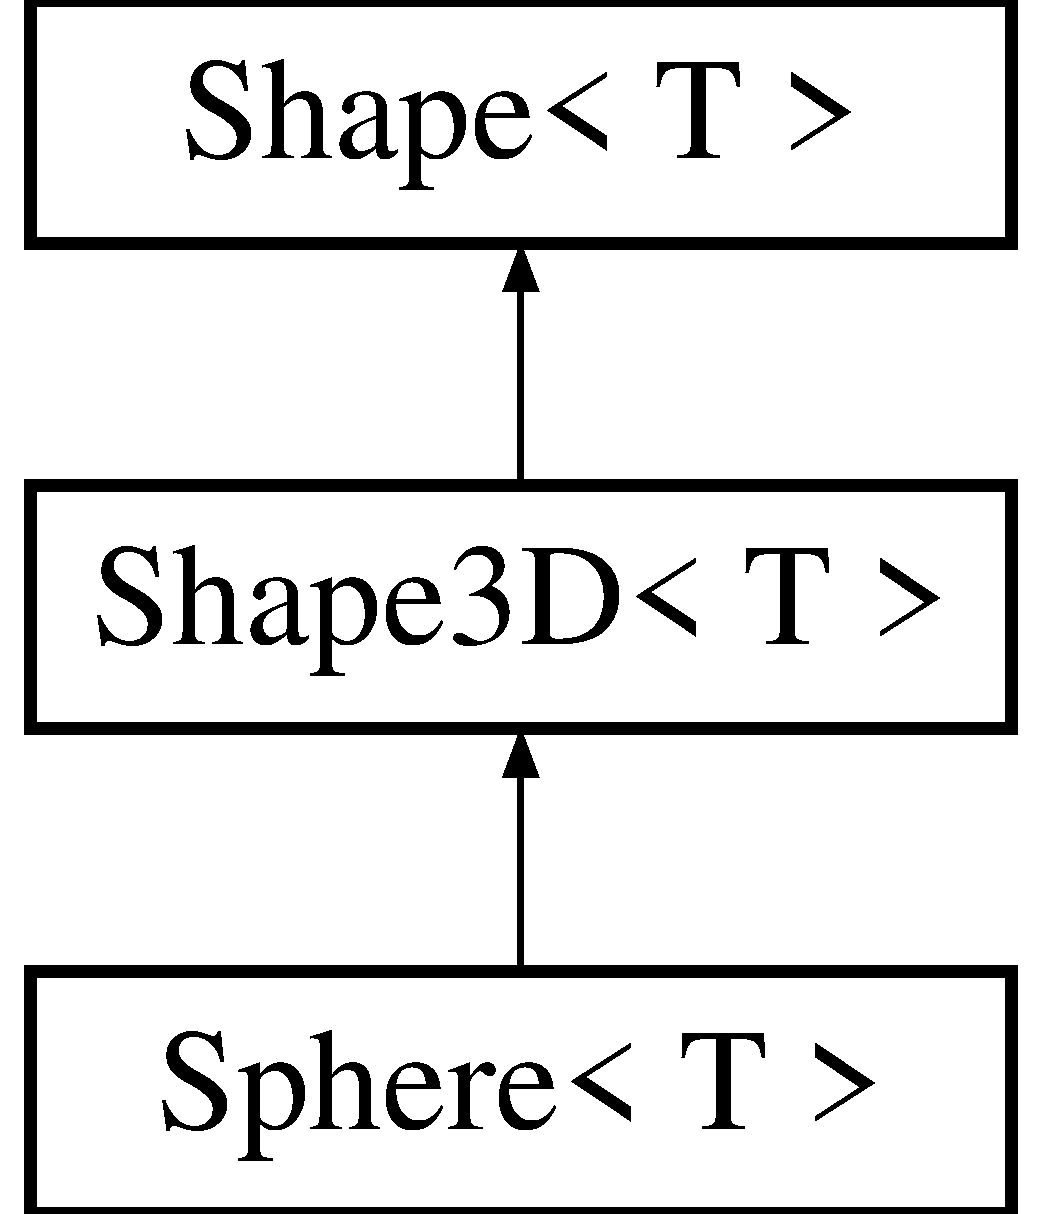
\includegraphics[height=3.000000cm]{classSphere}
\end{center}
\end{figure}
\subsection*{Public Member Functions}
\begin{DoxyCompactItemize}
\item 
\mbox{\hyperlink{classSphere_acacfd6de079ea50acdaf57b823166651}{Sphere}} ()
\begin{DoxyCompactList}\small\item\em \mbox{\hyperlink{classA}{A}} basic constructor for \mbox{\hyperlink{classSphere}{Sphere}} class. \end{DoxyCompactList}\item 
\mbox{\hyperlink{classSphere_a79e3c1cb536e3fe4d8bc447e7be0e414}{Sphere}} (int min\+\_\+vertexes\+\_\+)
\begin{DoxyCompactList}\small\item\em \mbox{\hyperlink{classA}{A}} basic constructor for \mbox{\hyperlink{classSphere}{Sphere}} class. \end{DoxyCompactList}\item 
\mbox{\hyperlink{classSphere_af0d667b078ae88955113205112d9aaa6}{Sphere}} (\mbox{\hyperlink{classSphere}{Sphere}} \&\&)=default
\item 
\mbox{\hyperlink{classSphere}{Sphere}} \& \mbox{\hyperlink{classSphere_aa117f966cea7b16532cbd80c2191a84a}{operator=}} (\mbox{\hyperlink{classSphere}{Sphere}} \&\&)=default
\item 
\mbox{\hyperlink{classSphere_ae28ad7649c59d653b9e14a3042d186a1}{Sphere}} (const \mbox{\hyperlink{classSphere}{Sphere}} \&)=default
\item 
\mbox{\hyperlink{classSphere}{Sphere}} \& \mbox{\hyperlink{classSphere_ae989d05c3ea71f5a758e90e2f2e3aecf}{operator=}} (const \mbox{\hyperlink{classSphere}{Sphere}} \&)=default
\item 
\mbox{\hyperlink{glad_8h_a950fc91edb4504f62f1c577bf4727c29}{void}} \mbox{\hyperlink{classSphere_a3f5ee2b07e48a360696fe983690d1d1f}{refine}} ()
\begin{DoxyCompactList}\small\item\em \mbox{\hyperlink{classThis}{This}} function calls generate\+\_\+vertexes\+\_\+helper to refine the mesh. \end{DoxyCompactList}\item 
T \mbox{\hyperlink{classSphere_a9ebc65dabaf8d87fbe599f4b64816f73}{quality}} ()
\begin{DoxyCompactList}\small\item\em The quality of the mesh is measured as the difference between exact pi number and the one obtained from the area of the sphere (mesh). \end{DoxyCompactList}\end{DoxyCompactItemize}
\subsection*{Private Member Functions}
\begin{DoxyCompactItemize}
\item 
\mbox{\hyperlink{glad_8h_a950fc91edb4504f62f1c577bf4727c29}{void}} \mbox{\hyperlink{classSphere_ab739ad1931e58a4ba7c84e3ca5c1965d}{generate\+\_\+vertexes\+\_\+helper\+\_\+old}} ()
\item 
\mbox{\hyperlink{glad_8h_a950fc91edb4504f62f1c577bf4727c29}{void}} \mbox{\hyperlink{classSphere_a84a45f41ca9e630beb97fc106b359ffd}{generate\+\_\+vertexes\+\_\+helper}} ()
\begin{DoxyCompactList}\small\item\em \mbox{\hyperlink{classThis}{This}} function generates vertexes for float and double version of class \mbox{\hyperlink{classCircle}{Circle}}. \end{DoxyCompactList}\item 
\mbox{\hyperlink{glad_8h_a950fc91edb4504f62f1c577bf4727c29}{void}} \mbox{\hyperlink{classSphere_a9cfac85b9803fadc4b79db0ea047f679}{generate\+\_\+vertexes}} ()
\begin{DoxyCompactList}\small\item\em \mbox{\hyperlink{classThis}{This}} function generates vertexes for class \mbox{\hyperlink{classCircle}{Circle}}. \end{DoxyCompactList}\end{DoxyCompactItemize}
\subsection*{Additional Inherited Members}


\subsection{Constructor \& Destructor Documentation}
\mbox{\Hypertarget{classSphere_acacfd6de079ea50acdaf57b823166651}\label{classSphere_acacfd6de079ea50acdaf57b823166651}} 
\index{Sphere@{Sphere}!Sphere@{Sphere}}
\index{Sphere@{Sphere}!Sphere@{Sphere}}
\subsubsection{\texorpdfstring{Sphere()}{Sphere()}\hspace{0.1cm}{\footnotesize\ttfamily [1/4]}}
{\footnotesize\ttfamily template$<$typename T = float$>$ \\
\mbox{\hyperlink{classSphere}{Sphere}}$<$ T $>$\+::\mbox{\hyperlink{classSphere}{Sphere}} (\begin{DoxyParamCaption}{ }\end{DoxyParamCaption})\hspace{0.3cm}{\ttfamily [inline]}}



\mbox{\hyperlink{classA}{A}} basic constructor for \mbox{\hyperlink{classSphere}{Sphere}} class. 

The constructor generate vertexes and elements. Opengl buffers are also allocated and initiallized. \mbox{\Hypertarget{classSphere_a79e3c1cb536e3fe4d8bc447e7be0e414}\label{classSphere_a79e3c1cb536e3fe4d8bc447e7be0e414}} 
\index{Sphere@{Sphere}!Sphere@{Sphere}}
\index{Sphere@{Sphere}!Sphere@{Sphere}}
\subsubsection{\texorpdfstring{Sphere()}{Sphere()}\hspace{0.1cm}{\footnotesize\ttfamily [2/4]}}
{\footnotesize\ttfamily template$<$typename T = float$>$ \\
\mbox{\hyperlink{classSphere}{Sphere}}$<$ T $>$\+::\mbox{\hyperlink{classSphere}{Sphere}} (\begin{DoxyParamCaption}\item[{int}]{min\+\_\+vertexes\+\_\+ }\end{DoxyParamCaption})\hspace{0.3cm}{\ttfamily [inline]}}



\mbox{\hyperlink{classA}{A}} basic constructor for \mbox{\hyperlink{classSphere}{Sphere}} class. 

The constructor generate vertexes and elements. Opengl buffers are also allocated and initiallized. 
\begin{DoxyParams}{Parameters}
{\em min\+\_\+vertexes\+\_\+} & minimal number of vertexes to create sphere \\
\hline
\end{DoxyParams}
\mbox{\Hypertarget{classSphere_af0d667b078ae88955113205112d9aaa6}\label{classSphere_af0d667b078ae88955113205112d9aaa6}} 
\index{Sphere@{Sphere}!Sphere@{Sphere}}
\index{Sphere@{Sphere}!Sphere@{Sphere}}
\subsubsection{\texorpdfstring{Sphere()}{Sphere()}\hspace{0.1cm}{\footnotesize\ttfamily [3/4]}}
{\footnotesize\ttfamily template$<$typename T = float$>$ \\
\mbox{\hyperlink{classSphere}{Sphere}}$<$ T $>$\+::\mbox{\hyperlink{classSphere}{Sphere}} (\begin{DoxyParamCaption}\item[{\mbox{\hyperlink{classSphere}{Sphere}}$<$ T $>$ \&\&}]{ }\end{DoxyParamCaption})\hspace{0.3cm}{\ttfamily [default]}}

\mbox{\Hypertarget{classSphere_ae28ad7649c59d653b9e14a3042d186a1}\label{classSphere_ae28ad7649c59d653b9e14a3042d186a1}} 
\index{Sphere@{Sphere}!Sphere@{Sphere}}
\index{Sphere@{Sphere}!Sphere@{Sphere}}
\subsubsection{\texorpdfstring{Sphere()}{Sphere()}\hspace{0.1cm}{\footnotesize\ttfamily [4/4]}}
{\footnotesize\ttfamily template$<$typename T = float$>$ \\
\mbox{\hyperlink{classSphere}{Sphere}}$<$ T $>$\+::\mbox{\hyperlink{classSphere}{Sphere}} (\begin{DoxyParamCaption}\item[{const \mbox{\hyperlink{classSphere}{Sphere}}$<$ T $>$ \&}]{ }\end{DoxyParamCaption})\hspace{0.3cm}{\ttfamily [default]}}



\subsection{Member Function Documentation}
\mbox{\Hypertarget{classSphere_a9cfac85b9803fadc4b79db0ea047f679}\label{classSphere_a9cfac85b9803fadc4b79db0ea047f679}} 
\index{Sphere@{Sphere}!generate\+\_\+vertexes@{generate\+\_\+vertexes}}
\index{generate\+\_\+vertexes@{generate\+\_\+vertexes}!Sphere@{Sphere}}
\subsubsection{\texorpdfstring{generate\+\_\+vertexes()}{generate\_vertexes()}}
{\footnotesize\ttfamily template$<$typename T $>$ \\
\mbox{\hyperlink{glad_8h_a950fc91edb4504f62f1c577bf4727c29}{void}} \mbox{\hyperlink{classSphere}{Sphere}}$<$ T $>$\+::generate\+\_\+vertexes (\begin{DoxyParamCaption}{ }\end{DoxyParamCaption})\hspace{0.3cm}{\ttfamily [private]}}



\mbox{\hyperlink{classThis}{This}} function generates vertexes for class \mbox{\hyperlink{classCircle}{Circle}}. 

Internally, it calls generate\+\_\+vertexes\+\_\+helper function to refine the mesh. \mbox{\Hypertarget{classSphere_a84a45f41ca9e630beb97fc106b359ffd}\label{classSphere_a84a45f41ca9e630beb97fc106b359ffd}} 
\index{Sphere@{Sphere}!generate\+\_\+vertexes\+\_\+helper@{generate\+\_\+vertexes\+\_\+helper}}
\index{generate\+\_\+vertexes\+\_\+helper@{generate\+\_\+vertexes\+\_\+helper}!Sphere@{Sphere}}
\subsubsection{\texorpdfstring{generate\+\_\+vertexes\+\_\+helper()}{generate\_vertexes\_helper()}}
{\footnotesize\ttfamily template$<$typename T $>$ \\
\mbox{\hyperlink{glad_8h_a950fc91edb4504f62f1c577bf4727c29}{void}} \mbox{\hyperlink{classSphere}{Sphere}}$<$ T $>$\+::generate\+\_\+vertexes\+\_\+helper (\begin{DoxyParamCaption}{ }\end{DoxyParamCaption})\hspace{0.3cm}{\ttfamily [inline]}, {\ttfamily [private]}}



\mbox{\hyperlink{classThis}{This}} function generates vertexes for float and double version of class \mbox{\hyperlink{classCircle}{Circle}}. 

It is used only when sse and avx versions are not available. \mbox{\Hypertarget{classSphere_ab739ad1931e58a4ba7c84e3ca5c1965d}\label{classSphere_ab739ad1931e58a4ba7c84e3ca5c1965d}} 
\index{Sphere@{Sphere}!generate\+\_\+vertexes\+\_\+helper\+\_\+old@{generate\+\_\+vertexes\+\_\+helper\+\_\+old}}
\index{generate\+\_\+vertexes\+\_\+helper\+\_\+old@{generate\+\_\+vertexes\+\_\+helper\+\_\+old}!Sphere@{Sphere}}
\subsubsection{\texorpdfstring{generate\+\_\+vertexes\+\_\+helper\+\_\+old()}{generate\_vertexes\_helper\_old()}}
{\footnotesize\ttfamily template$<$typename T = float$>$ \\
\mbox{\hyperlink{glad_8h_a950fc91edb4504f62f1c577bf4727c29}{void}} \mbox{\hyperlink{classSphere}{Sphere}}$<$ T $>$\+::generate\+\_\+vertexes\+\_\+helper\+\_\+old (\begin{DoxyParamCaption}{ }\end{DoxyParamCaption})\hspace{0.3cm}{\ttfamily [private]}}

\mbox{\Hypertarget{classSphere_aa117f966cea7b16532cbd80c2191a84a}\label{classSphere_aa117f966cea7b16532cbd80c2191a84a}} 
\index{Sphere@{Sphere}!operator=@{operator=}}
\index{operator=@{operator=}!Sphere@{Sphere}}
\subsubsection{\texorpdfstring{operator=()}{operator=()}\hspace{0.1cm}{\footnotesize\ttfamily [1/2]}}
{\footnotesize\ttfamily template$<$typename T = float$>$ \\
\mbox{\hyperlink{classSphere}{Sphere}}\& \mbox{\hyperlink{classSphere}{Sphere}}$<$ T $>$\+::operator= (\begin{DoxyParamCaption}\item[{\mbox{\hyperlink{classSphere}{Sphere}}$<$ T $>$ \&\&}]{ }\end{DoxyParamCaption})\hspace{0.3cm}{\ttfamily [default]}}

\mbox{\Hypertarget{classSphere_ae989d05c3ea71f5a758e90e2f2e3aecf}\label{classSphere_ae989d05c3ea71f5a758e90e2f2e3aecf}} 
\index{Sphere@{Sphere}!operator=@{operator=}}
\index{operator=@{operator=}!Sphere@{Sphere}}
\subsubsection{\texorpdfstring{operator=()}{operator=()}\hspace{0.1cm}{\footnotesize\ttfamily [2/2]}}
{\footnotesize\ttfamily template$<$typename T = float$>$ \\
\mbox{\hyperlink{classSphere}{Sphere}}\& \mbox{\hyperlink{classSphere}{Sphere}}$<$ T $>$\+::operator= (\begin{DoxyParamCaption}\item[{const \mbox{\hyperlink{classSphere}{Sphere}}$<$ T $>$ \&}]{ }\end{DoxyParamCaption})\hspace{0.3cm}{\ttfamily [default]}}

\mbox{\Hypertarget{classSphere_a9ebc65dabaf8d87fbe599f4b64816f73}\label{classSphere_a9ebc65dabaf8d87fbe599f4b64816f73}} 
\index{Sphere@{Sphere}!quality@{quality}}
\index{quality@{quality}!Sphere@{Sphere}}
\subsubsection{\texorpdfstring{quality()}{quality()}}
{\footnotesize\ttfamily template$<$typename T $>$ \\
T \mbox{\hyperlink{classSphere}{Sphere}}$<$ T $>$\+::quality (\begin{DoxyParamCaption}{ }\end{DoxyParamCaption})}



The quality of the mesh is measured as the difference between exact pi number and the one obtained from the area of the sphere (mesh). 

\mbox{\Hypertarget{classSphere_a3f5ee2b07e48a360696fe983690d1d1f}\label{classSphere_a3f5ee2b07e48a360696fe983690d1d1f}} 
\index{Sphere@{Sphere}!refine@{refine}}
\index{refine@{refine}!Sphere@{Sphere}}
\subsubsection{\texorpdfstring{refine()}{refine()}}
{\footnotesize\ttfamily template$<$typename T $>$ \\
\mbox{\hyperlink{glad_8h_a950fc91edb4504f62f1c577bf4727c29}{void}} \mbox{\hyperlink{classSphere}{Sphere}}$<$ T $>$\+::refine (\begin{DoxyParamCaption}{ }\end{DoxyParamCaption})}



\mbox{\hyperlink{classThis}{This}} function calls generate\+\_\+vertexes\+\_\+helper to refine the mesh. 



The documentation for this class was generated from the following file\+:\begin{DoxyCompactItemize}
\item 
src/shapes/\mbox{\hyperlink{sphere_8hpp}{sphere.\+hpp}}\end{DoxyCompactItemize}

\hypertarget{classStar}{}\section{Star$<$ T $>$ Class Template Reference}
\label{classStar}\index{Star$<$ T $>$@{Star$<$ T $>$}}


{\ttfamily \#include \char`\"{}star.\+hpp\char`\"{}}

Inheritance diagram for Star$<$ T $>$\+:\begin{figure}[H]
\begin{center}
\leavevmode
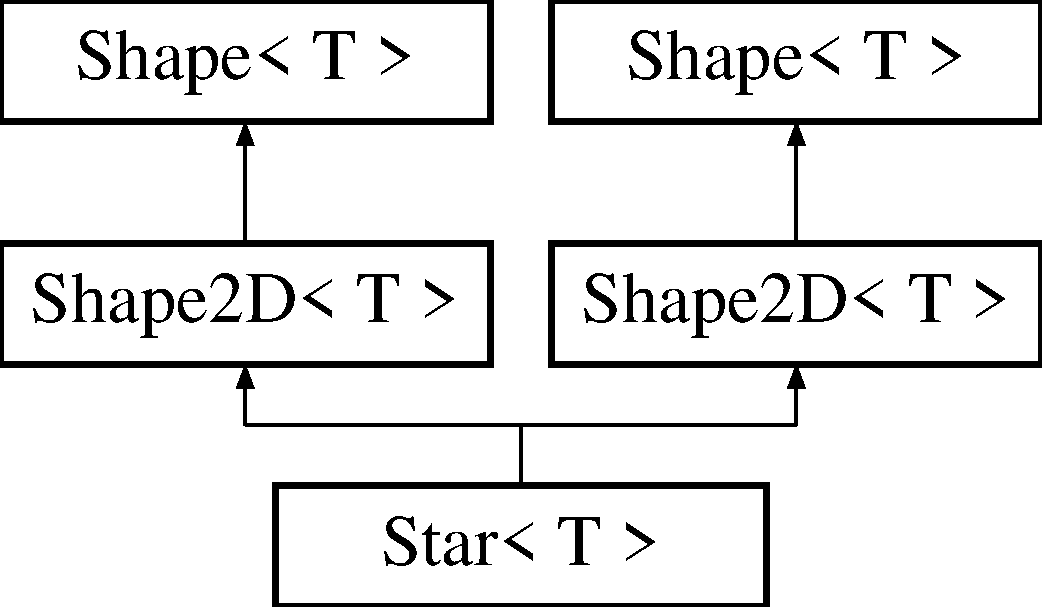
\includegraphics[height=3.000000cm]{classStar}
\end{center}
\end{figure}
\subsection*{Public Member Functions}
\begin{DoxyCompactItemize}
\item 
\mbox{\hyperlink{classStar_a4be07c82320f781071409294614df4ae}{Star}} ()
\item 
\mbox{\hyperlink{classStar_aa179936ed93e38e70992cb4f6e3cbff3}{Star}} (int, T=0.\+5)
\item 
\mbox{\hyperlink{classStar_af518471484341cad6b47ad42d4e637fe}{Star}} (\mbox{\hyperlink{classStar}{Star}} \&\&)=default
\item 
\mbox{\hyperlink{classStar}{Star}} \& \mbox{\hyperlink{classStar_a7113d2808314f0aa2f5a87325f8c535d}{operator=}} (\mbox{\hyperlink{classStar}{Star}} \&\&)=default
\item 
\mbox{\hyperlink{classStar_a047ce2a8d4fb409858555aee98b33c93}{Star}} (const \mbox{\hyperlink{classStar}{Star}} \&)=default
\item 
\mbox{\hyperlink{classStar}{Star}} \& \mbox{\hyperlink{classStar_a3507f157448e082ccfcadc4783f2610e}{operator=}} (const \mbox{\hyperlink{classStar}{Star}} \&)=default
\item 
T \mbox{\hyperlink{classStar_a908253192d0b1fe95aeeaa81322545bf}{perimeter}} ()
\item 
\mbox{\hyperlink{classStar_a4be07c82320f781071409294614df4ae}{Star}} ()
\item 
\mbox{\hyperlink{classStar_aa179936ed93e38e70992cb4f6e3cbff3}{Star}} (int, T=0.\+5)
\item 
\mbox{\hyperlink{classStar_af518471484341cad6b47ad42d4e637fe}{Star}} (\mbox{\hyperlink{classStar}{Star}} \&\&)=default
\item 
\mbox{\hyperlink{classStar}{Star}} \& \mbox{\hyperlink{classStar_a7113d2808314f0aa2f5a87325f8c535d}{operator=}} (\mbox{\hyperlink{classStar}{Star}} \&\&)=default
\item 
\mbox{\hyperlink{classStar_a047ce2a8d4fb409858555aee98b33c93}{Star}} (const \mbox{\hyperlink{classStar}{Star}} \&)=default
\item 
\mbox{\hyperlink{classStar}{Star}} \& \mbox{\hyperlink{classStar_a3507f157448e082ccfcadc4783f2610e}{operator=}} (const \mbox{\hyperlink{classStar}{Star}} \&)=default
\item 
T \mbox{\hyperlink{classStar_a908253192d0b1fe95aeeaa81322545bf}{perimeter}} ()
\end{DoxyCompactItemize}
\subsection*{Public Attributes}
\begin{DoxyCompactItemize}
\item 
T \mbox{\hyperlink{classStar_a349e0820769da7e4f76aea0ad6002bf8}{ratio}}
\end{DoxyCompactItemize}
\subsection*{Private Member Functions}
\begin{DoxyCompactItemize}
\item 
void \mbox{\hyperlink{classStar_ac9ce42a8f7289484594f7f0ab5124849}{generate\+\_\+vertexes}} (int=10, T=0.\+5)
\item 
void \mbox{\hyperlink{classStar_ac9ce42a8f7289484594f7f0ab5124849}{generate\+\_\+vertexes}} (int=10, T=0.\+5)
\item 
{\footnotesize template$<$$>$ }\\void \mbox{\hyperlink{classStar_ab46cbc7aca971bc1c07b8d4afe8fba37}{generate\+\_\+vertexes}} (int bulges, float \mbox{\hyperlink{classStar_a349e0820769da7e4f76aea0ad6002bf8}{ratio}})
\item 
{\footnotesize template$<$$>$ }\\void \mbox{\hyperlink{classStar_a85d8438cea72701a136b76f046ee95dd}{generate\+\_\+vertexes}} (int bulges, double \mbox{\hyperlink{classStar_a349e0820769da7e4f76aea0ad6002bf8}{ratio}})
\item 
{\footnotesize template$<$$>$ }\\void \mbox{\hyperlink{classStar_ab46cbc7aca971bc1c07b8d4afe8fba37}{generate\+\_\+vertexes}} (int bulges, float \mbox{\hyperlink{classStar_a349e0820769da7e4f76aea0ad6002bf8}{ratio}})
\item 
{\footnotesize template$<$$>$ }\\void \mbox{\hyperlink{classStar_a85d8438cea72701a136b76f046ee95dd}{generate\+\_\+vertexes}} (int bulges, double \mbox{\hyperlink{classStar_a349e0820769da7e4f76aea0ad6002bf8}{ratio}})
\end{DoxyCompactItemize}
\subsection*{Additional Inherited Members}


\subsection{Constructor \& Destructor Documentation}
\mbox{\Hypertarget{classStar_a4be07c82320f781071409294614df4ae}\label{classStar_a4be07c82320f781071409294614df4ae}} 
\index{Star@{Star}!Star@{Star}}
\index{Star@{Star}!Star@{Star}}
\subsubsection{\texorpdfstring{Star()}{Star()}\hspace{0.1cm}{\footnotesize\ttfamily [1/8]}}
{\footnotesize\ttfamily template$<$typename T $>$ \\
\mbox{\hyperlink{classStar}{Star}}$<$ T $>$\+::\mbox{\hyperlink{classStar}{Star}} (\begin{DoxyParamCaption}{ }\end{DoxyParamCaption})}

\mbox{\Hypertarget{classStar_aa179936ed93e38e70992cb4f6e3cbff3}\label{classStar_aa179936ed93e38e70992cb4f6e3cbff3}} 
\index{Star@{Star}!Star@{Star}}
\index{Star@{Star}!Star@{Star}}
\subsubsection{\texorpdfstring{Star()}{Star()}\hspace{0.1cm}{\footnotesize\ttfamily [2/8]}}
{\footnotesize\ttfamily template$<$typename T $>$ \\
\mbox{\hyperlink{classStar}{Star}}$<$ T $>$\+::\mbox{\hyperlink{classStar}{Star}} (\begin{DoxyParamCaption}\item[{int}]{bulges,  }\item[{T}]{ratio = {\ttfamily 0.5} }\end{DoxyParamCaption})}

\mbox{\Hypertarget{classStar_af518471484341cad6b47ad42d4e637fe}\label{classStar_af518471484341cad6b47ad42d4e637fe}} 
\index{Star@{Star}!Star@{Star}}
\index{Star@{Star}!Star@{Star}}
\subsubsection{\texorpdfstring{Star()}{Star()}\hspace{0.1cm}{\footnotesize\ttfamily [3/8]}}
{\footnotesize\ttfamily template$<$typename T  = float$>$ \\
\mbox{\hyperlink{classStar}{Star}}$<$ T $>$\+::\mbox{\hyperlink{classStar}{Star}} (\begin{DoxyParamCaption}\item[{\mbox{\hyperlink{classStar}{Star}}$<$ T $>$ \&\&}]{ }\end{DoxyParamCaption})\hspace{0.3cm}{\ttfamily [default]}}

\mbox{\Hypertarget{classStar_a047ce2a8d4fb409858555aee98b33c93}\label{classStar_a047ce2a8d4fb409858555aee98b33c93}} 
\index{Star@{Star}!Star@{Star}}
\index{Star@{Star}!Star@{Star}}
\subsubsection{\texorpdfstring{Star()}{Star()}\hspace{0.1cm}{\footnotesize\ttfamily [4/8]}}
{\footnotesize\ttfamily template$<$typename T  = float$>$ \\
\mbox{\hyperlink{classStar}{Star}}$<$ T $>$\+::\mbox{\hyperlink{classStar}{Star}} (\begin{DoxyParamCaption}\item[{const \mbox{\hyperlink{classStar}{Star}}$<$ T $>$ \&}]{ }\end{DoxyParamCaption})\hspace{0.3cm}{\ttfamily [default]}}

\mbox{\Hypertarget{classStar_a4be07c82320f781071409294614df4ae}\label{classStar_a4be07c82320f781071409294614df4ae}} 
\index{Star@{Star}!Star@{Star}}
\index{Star@{Star}!Star@{Star}}
\subsubsection{\texorpdfstring{Star()}{Star()}\hspace{0.1cm}{\footnotesize\ttfamily [5/8]}}
{\footnotesize\ttfamily template$<$typename T  = float$>$ \\
\mbox{\hyperlink{classStar}{Star}}$<$ T $>$\+::\mbox{\hyperlink{classStar}{Star}} (\begin{DoxyParamCaption}{ }\end{DoxyParamCaption})}

\mbox{\Hypertarget{classStar_aa179936ed93e38e70992cb4f6e3cbff3}\label{classStar_aa179936ed93e38e70992cb4f6e3cbff3}} 
\index{Star@{Star}!Star@{Star}}
\index{Star@{Star}!Star@{Star}}
\subsubsection{\texorpdfstring{Star()}{Star()}\hspace{0.1cm}{\footnotesize\ttfamily [6/8]}}
{\footnotesize\ttfamily template$<$typename T  = float$>$ \\
\mbox{\hyperlink{classStar}{Star}}$<$ T $>$\+::\mbox{\hyperlink{classStar}{Star}} (\begin{DoxyParamCaption}\item[{int}]{,  }\item[{T}]{ = {\ttfamily 0.5} }\end{DoxyParamCaption})}

\mbox{\Hypertarget{classStar_af518471484341cad6b47ad42d4e637fe}\label{classStar_af518471484341cad6b47ad42d4e637fe}} 
\index{Star@{Star}!Star@{Star}}
\index{Star@{Star}!Star@{Star}}
\subsubsection{\texorpdfstring{Star()}{Star()}\hspace{0.1cm}{\footnotesize\ttfamily [7/8]}}
{\footnotesize\ttfamily template$<$typename T  = float$>$ \\
\mbox{\hyperlink{classStar}{Star}}$<$ T $>$\+::\mbox{\hyperlink{classStar}{Star}} (\begin{DoxyParamCaption}\item[{\mbox{\hyperlink{classStar}{Star}}$<$ T $>$ \&\&}]{ }\end{DoxyParamCaption})\hspace{0.3cm}{\ttfamily [default]}}

\mbox{\Hypertarget{classStar_a047ce2a8d4fb409858555aee98b33c93}\label{classStar_a047ce2a8d4fb409858555aee98b33c93}} 
\index{Star@{Star}!Star@{Star}}
\index{Star@{Star}!Star@{Star}}
\subsubsection{\texorpdfstring{Star()}{Star()}\hspace{0.1cm}{\footnotesize\ttfamily [8/8]}}
{\footnotesize\ttfamily template$<$typename T  = float$>$ \\
\mbox{\hyperlink{classStar}{Star}}$<$ T $>$\+::\mbox{\hyperlink{classStar}{Star}} (\begin{DoxyParamCaption}\item[{const \mbox{\hyperlink{classStar}{Star}}$<$ T $>$ \&}]{ }\end{DoxyParamCaption})\hspace{0.3cm}{\ttfamily [default]}}



\subsection{Member Function Documentation}
\mbox{\Hypertarget{classStar_ac9ce42a8f7289484594f7f0ab5124849}\label{classStar_ac9ce42a8f7289484594f7f0ab5124849}} 
\index{Star@{Star}!generate\+\_\+vertexes@{generate\+\_\+vertexes}}
\index{generate\+\_\+vertexes@{generate\+\_\+vertexes}!Star@{Star}}
\subsubsection{\texorpdfstring{generate\+\_\+vertexes()}{generate\_vertexes()}\hspace{0.1cm}{\footnotesize\ttfamily [1/6]}}
{\footnotesize\ttfamily template$<$typename T  = float$>$ \\
void \mbox{\hyperlink{classStar}{Star}}$<$ T $>$\+::generate\+\_\+vertexes (\begin{DoxyParamCaption}\item[{int}]{ = {\ttfamily 10},  }\item[{T}]{ = {\ttfamily 0.5} }\end{DoxyParamCaption})\hspace{0.3cm}{\ttfamily [private]}}

\mbox{\Hypertarget{classStar_ac9ce42a8f7289484594f7f0ab5124849}\label{classStar_ac9ce42a8f7289484594f7f0ab5124849}} 
\index{Star@{Star}!generate\+\_\+vertexes@{generate\+\_\+vertexes}}
\index{generate\+\_\+vertexes@{generate\+\_\+vertexes}!Star@{Star}}
\subsubsection{\texorpdfstring{generate\+\_\+vertexes()}{generate\_vertexes()}\hspace{0.1cm}{\footnotesize\ttfamily [2/6]}}
{\footnotesize\ttfamily template$<$typename T  = float$>$ \\
void \mbox{\hyperlink{classStar}{Star}}$<$ T $>$\+::generate\+\_\+vertexes (\begin{DoxyParamCaption}\item[{int}]{ = {\ttfamily 10},  }\item[{T}]{ = {\ttfamily 0.5} }\end{DoxyParamCaption})\hspace{0.3cm}{\ttfamily [private]}}

\mbox{\Hypertarget{classStar_ab46cbc7aca971bc1c07b8d4afe8fba37}\label{classStar_ab46cbc7aca971bc1c07b8d4afe8fba37}} 
\index{Star@{Star}!generate\+\_\+vertexes@{generate\+\_\+vertexes}}
\index{generate\+\_\+vertexes@{generate\+\_\+vertexes}!Star@{Star}}
\subsubsection{\texorpdfstring{generate\+\_\+vertexes()}{generate\_vertexes()}\hspace{0.1cm}{\footnotesize\ttfamily [3/6]}}
{\footnotesize\ttfamily template$<$$>$ \\
void \mbox{\hyperlink{classStar}{Star}}$<$ float $>$\+::generate\+\_\+vertexes (\begin{DoxyParamCaption}\item[{int}]{bulges,  }\item[{float}]{ratio }\end{DoxyParamCaption})\hspace{0.3cm}{\ttfamily [inline]}, {\ttfamily [private]}}

\mbox{\Hypertarget{classStar_ab46cbc7aca971bc1c07b8d4afe8fba37}\label{classStar_ab46cbc7aca971bc1c07b8d4afe8fba37}} 
\index{Star@{Star}!generate\+\_\+vertexes@{generate\+\_\+vertexes}}
\index{generate\+\_\+vertexes@{generate\+\_\+vertexes}!Star@{Star}}
\subsubsection{\texorpdfstring{generate\+\_\+vertexes()}{generate\_vertexes()}\hspace{0.1cm}{\footnotesize\ttfamily [4/6]}}
{\footnotesize\ttfamily template$<$$>$ \\
void \mbox{\hyperlink{classStar}{Star}}$<$ float $>$\+::generate\+\_\+vertexes (\begin{DoxyParamCaption}\item[{int}]{bulges,  }\item[{float}]{ratio }\end{DoxyParamCaption})\hspace{0.3cm}{\ttfamily [inline]}, {\ttfamily [private]}}

\mbox{\Hypertarget{classStar_a85d8438cea72701a136b76f046ee95dd}\label{classStar_a85d8438cea72701a136b76f046ee95dd}} 
\index{Star@{Star}!generate\+\_\+vertexes@{generate\+\_\+vertexes}}
\index{generate\+\_\+vertexes@{generate\+\_\+vertexes}!Star@{Star}}
\subsubsection{\texorpdfstring{generate\+\_\+vertexes()}{generate\_vertexes()}\hspace{0.1cm}{\footnotesize\ttfamily [5/6]}}
{\footnotesize\ttfamily template$<$$>$ \\
void \mbox{\hyperlink{classStar}{Star}}$<$ double $>$\+::generate\+\_\+vertexes (\begin{DoxyParamCaption}\item[{int}]{bulges,  }\item[{double}]{ratio }\end{DoxyParamCaption})\hspace{0.3cm}{\ttfamily [inline]}, {\ttfamily [private]}}

\mbox{\Hypertarget{classStar_a85d8438cea72701a136b76f046ee95dd}\label{classStar_a85d8438cea72701a136b76f046ee95dd}} 
\index{Star@{Star}!generate\+\_\+vertexes@{generate\+\_\+vertexes}}
\index{generate\+\_\+vertexes@{generate\+\_\+vertexes}!Star@{Star}}
\subsubsection{\texorpdfstring{generate\+\_\+vertexes()}{generate\_vertexes()}\hspace{0.1cm}{\footnotesize\ttfamily [6/6]}}
{\footnotesize\ttfamily template$<$$>$ \\
void \mbox{\hyperlink{classStar}{Star}}$<$ double $>$\+::generate\+\_\+vertexes (\begin{DoxyParamCaption}\item[{int}]{bulges,  }\item[{double}]{ratio }\end{DoxyParamCaption})\hspace{0.3cm}{\ttfamily [inline]}, {\ttfamily [private]}}

\mbox{\Hypertarget{classStar_a7113d2808314f0aa2f5a87325f8c535d}\label{classStar_a7113d2808314f0aa2f5a87325f8c535d}} 
\index{Star@{Star}!operator=@{operator=}}
\index{operator=@{operator=}!Star@{Star}}
\subsubsection{\texorpdfstring{operator=()}{operator=()}\hspace{0.1cm}{\footnotesize\ttfamily [1/4]}}
{\footnotesize\ttfamily template$<$typename T  = float$>$ \\
\mbox{\hyperlink{classStar}{Star}}\& \mbox{\hyperlink{classStar}{Star}}$<$ T $>$\+::operator= (\begin{DoxyParamCaption}\item[{\mbox{\hyperlink{classStar}{Star}}$<$ T $>$ \&\&}]{ }\end{DoxyParamCaption})\hspace{0.3cm}{\ttfamily [default]}}

\mbox{\Hypertarget{classStar_a7113d2808314f0aa2f5a87325f8c535d}\label{classStar_a7113d2808314f0aa2f5a87325f8c535d}} 
\index{Star@{Star}!operator=@{operator=}}
\index{operator=@{operator=}!Star@{Star}}
\subsubsection{\texorpdfstring{operator=()}{operator=()}\hspace{0.1cm}{\footnotesize\ttfamily [2/4]}}
{\footnotesize\ttfamily template$<$typename T  = float$>$ \\
\mbox{\hyperlink{classStar}{Star}}\& \mbox{\hyperlink{classStar}{Star}}$<$ T $>$\+::operator= (\begin{DoxyParamCaption}\item[{\mbox{\hyperlink{classStar}{Star}}$<$ T $>$ \&\&}]{ }\end{DoxyParamCaption})\hspace{0.3cm}{\ttfamily [default]}}

\mbox{\Hypertarget{classStar_a3507f157448e082ccfcadc4783f2610e}\label{classStar_a3507f157448e082ccfcadc4783f2610e}} 
\index{Star@{Star}!operator=@{operator=}}
\index{operator=@{operator=}!Star@{Star}}
\subsubsection{\texorpdfstring{operator=()}{operator=()}\hspace{0.1cm}{\footnotesize\ttfamily [3/4]}}
{\footnotesize\ttfamily template$<$typename T  = float$>$ \\
\mbox{\hyperlink{classStar}{Star}}\& \mbox{\hyperlink{classStar}{Star}}$<$ T $>$\+::operator= (\begin{DoxyParamCaption}\item[{const \mbox{\hyperlink{classStar}{Star}}$<$ T $>$ \&}]{ }\end{DoxyParamCaption})\hspace{0.3cm}{\ttfamily [default]}}

\mbox{\Hypertarget{classStar_a3507f157448e082ccfcadc4783f2610e}\label{classStar_a3507f157448e082ccfcadc4783f2610e}} 
\index{Star@{Star}!operator=@{operator=}}
\index{operator=@{operator=}!Star@{Star}}
\subsubsection{\texorpdfstring{operator=()}{operator=()}\hspace{0.1cm}{\footnotesize\ttfamily [4/4]}}
{\footnotesize\ttfamily template$<$typename T  = float$>$ \\
\mbox{\hyperlink{classStar}{Star}}\& \mbox{\hyperlink{classStar}{Star}}$<$ T $>$\+::operator= (\begin{DoxyParamCaption}\item[{const \mbox{\hyperlink{classStar}{Star}}$<$ T $>$ \&}]{ }\end{DoxyParamCaption})\hspace{0.3cm}{\ttfamily [default]}}

\mbox{\Hypertarget{classStar_a908253192d0b1fe95aeeaa81322545bf}\label{classStar_a908253192d0b1fe95aeeaa81322545bf}} 
\index{Star@{Star}!perimeter@{perimeter}}
\index{perimeter@{perimeter}!Star@{Star}}
\subsubsection{\texorpdfstring{perimeter()}{perimeter()}\hspace{0.1cm}{\footnotesize\ttfamily [1/2]}}
{\footnotesize\ttfamily template$<$typename T  = float$>$ \\
T \mbox{\hyperlink{classStar}{Star}}$<$ T $>$\+::perimeter (\begin{DoxyParamCaption}{ }\end{DoxyParamCaption})}

\mbox{\Hypertarget{classStar_a908253192d0b1fe95aeeaa81322545bf}\label{classStar_a908253192d0b1fe95aeeaa81322545bf}} 
\index{Star@{Star}!perimeter@{perimeter}}
\index{perimeter@{perimeter}!Star@{Star}}
\subsubsection{\texorpdfstring{perimeter()}{perimeter()}\hspace{0.1cm}{\footnotesize\ttfamily [2/2]}}
{\footnotesize\ttfamily template$<$typename T  = float$>$ \\
T \mbox{\hyperlink{classStar}{Star}}$<$ T $>$\+::perimeter (\begin{DoxyParamCaption}{ }\end{DoxyParamCaption})}



\subsection{Member Data Documentation}
\mbox{\Hypertarget{classStar_a349e0820769da7e4f76aea0ad6002bf8}\label{classStar_a349e0820769da7e4f76aea0ad6002bf8}} 
\index{Star@{Star}!ratio@{ratio}}
\index{ratio@{ratio}!Star@{Star}}
\subsubsection{\texorpdfstring{ratio}{ratio}}
{\footnotesize\ttfamily template$<$typename T  = float$>$ \\
T \mbox{\hyperlink{classStar}{Star}}$<$ T $>$\+::ratio}



The documentation for this class was generated from the following files\+:\begin{DoxyCompactItemize}
\item 
src/\mbox{\hyperlink{star_8hpp}{star.\+hpp}}\item 
src/\mbox{\hyperlink{star3d_8hpp}{star3d.\+hpp}}\end{DoxyCompactItemize}

\hypertarget{classThis}{}\section{This Class Reference}
\label{classThis}\index{This@{This}}


\subsection{Detailed Description}
vertex and element data for 3d sphere. 

The documentation for this class was generated from the following file\+:\begin{DoxyCompactItemize}
\item 
src/shapes/\mbox{\hyperlink{sphere_8hpp}{sphere.\+hpp}}\end{DoxyCompactItemize}

\chapter{File Documentation}
\hypertarget{CMakeCCompilerId_8c}{}\section{build/\+C\+Make\+Files/3.12.3/\+Compiler\+Id\+C/\+C\+Make\+C\+Compiler\+Id.c File Reference}
\label{CMakeCCompilerId_8c}\index{build/\+C\+Make\+Files/3.\+12.\+3/\+Compiler\+Id\+C/\+C\+Make\+C\+Compiler\+Id.\+c@{build/\+C\+Make\+Files/3.\+12.\+3/\+Compiler\+Id\+C/\+C\+Make\+C\+Compiler\+Id.\+c}}
\subsection*{Macros}
\begin{DoxyCompactItemize}
\item 
\#define \mbox{\hyperlink{CMakeCCompilerId_8c_a81dee0709ded976b2e0319239f72d174}{C\+O\+M\+P\+I\+L\+E\+R\+\_\+\+ID}}~\char`\"{}\char`\"{}
\item 
\#define \mbox{\hyperlink{CMakeCCompilerId_8c_a2ae9b72bb13abaabfcf2ee0ba7d3fa1d}{S\+T\+R\+I\+N\+G\+I\+F\+Y\+\_\+\+H\+E\+L\+P\+ER}}(X)~\#X
\item 
\#define \mbox{\hyperlink{CMakeCCompilerId_8c_a43e1cad902b6477bec893cb6430bd6c8}{S\+T\+R\+I\+N\+G\+I\+FY}}(X)~\mbox{\hyperlink{CMakeCXXCompilerId_8cpp_a2ae9b72bb13abaabfcf2ee0ba7d3fa1d}{S\+T\+R\+I\+N\+G\+I\+F\+Y\+\_\+\+H\+E\+L\+P\+ER}}(X)
\item 
\#define \mbox{\hyperlink{CMakeCCompilerId_8c_adbc5372f40838899018fadbc89bd588b}{P\+L\+A\+T\+F\+O\+R\+M\+\_\+\+ID}}
\item 
\#define \mbox{\hyperlink{CMakeCCompilerId_8c_aba35d0d200deaeb06aee95ca297acb28}{A\+R\+C\+H\+I\+T\+E\+C\+T\+U\+R\+E\+\_\+\+ID}}
\item 
\#define \mbox{\hyperlink{CMakeCCompilerId_8c_ad1280362da42492bbc11aa78cbf776ad}{D\+EC}}(n)
\item 
\#define \mbox{\hyperlink{CMakeCCompilerId_8c_a46d5d95daa1bef867bd0179594310ed5}{H\+EX}}(n)
\item 
\#define \mbox{\hyperlink{CMakeCCompilerId_8c_a07f8e5783674099cd7f5110e22a78cdb}{C\+\_\+\+D\+I\+A\+L\+E\+CT}}
\end{DoxyCompactItemize}
\subsection*{Functions}
\begin{DoxyCompactItemize}
\item 
int \mbox{\hyperlink{CMakeCCompilerId_8c_a0ddf1224851353fc92bfbff6f499fa97}{main}} (int argc, char $\ast$argv\mbox{[}$\,$\mbox{]})
\end{DoxyCompactItemize}
\subsection*{Variables}
\begin{DoxyCompactItemize}
\item 
char const  $\ast$ \mbox{\hyperlink{CMakeCCompilerId_8c_a4b0efeb7a5d59313986b3a0390f050f6}{info\+\_\+compiler}} = \char`\"{}I\+N\+FO\char`\"{} \char`\"{}\+:\char`\"{} \char`\"{}compiler\mbox{[}\char`\"{} C\+O\+M\+P\+I\+L\+E\+R\+\_\+\+ID \char`\"{}\mbox{]}\char`\"{}
\item 
char const  $\ast$ \mbox{\hyperlink{CMakeCCompilerId_8c_a2321403dee54ee23f0c2fa849c60f7d4}{info\+\_\+platform}} = \char`\"{}I\+N\+FO\char`\"{} \char`\"{}\+:\char`\"{} \char`\"{}platform\mbox{[}\char`\"{} P\+L\+A\+T\+F\+O\+R\+M\+\_\+\+ID \char`\"{}\mbox{]}\char`\"{}
\item 
char const  $\ast$ \mbox{\hyperlink{CMakeCCompilerId_8c_a59647e99d304ed33b15cb284c27ed391}{info\+\_\+arch}} = \char`\"{}I\+N\+FO\char`\"{} \char`\"{}\+:\char`\"{} \char`\"{}arch\mbox{[}\char`\"{} A\+R\+C\+H\+I\+T\+E\+C\+T\+U\+R\+E\+\_\+\+ID \char`\"{}\mbox{]}\char`\"{}
\item 
const char $\ast$ \mbox{\hyperlink{CMakeCCompilerId_8c_a1ce162bad2fe6966ac8b33cc19e120b8}{info\+\_\+language\+\_\+dialect\+\_\+default}}
\end{DoxyCompactItemize}


\subsection{Macro Definition Documentation}
\mbox{\Hypertarget{CMakeCCompilerId_8c_aba35d0d200deaeb06aee95ca297acb28}\label{CMakeCCompilerId_8c_aba35d0d200deaeb06aee95ca297acb28}} 
\index{C\+Make\+C\+Compiler\+Id.\+c@{C\+Make\+C\+Compiler\+Id.\+c}!A\+R\+C\+H\+I\+T\+E\+C\+T\+U\+R\+E\+\_\+\+ID@{A\+R\+C\+H\+I\+T\+E\+C\+T\+U\+R\+E\+\_\+\+ID}}
\index{A\+R\+C\+H\+I\+T\+E\+C\+T\+U\+R\+E\+\_\+\+ID@{A\+R\+C\+H\+I\+T\+E\+C\+T\+U\+R\+E\+\_\+\+ID}!C\+Make\+C\+Compiler\+Id.\+c@{C\+Make\+C\+Compiler\+Id.\+c}}
\subsubsection{\texorpdfstring{A\+R\+C\+H\+I\+T\+E\+C\+T\+U\+R\+E\+\_\+\+ID}{ARCHITECTURE\_ID}}
{\footnotesize\ttfamily \#define A\+R\+C\+H\+I\+T\+E\+C\+T\+U\+R\+E\+\_\+\+ID}

\mbox{\Hypertarget{CMakeCCompilerId_8c_a07f8e5783674099cd7f5110e22a78cdb}\label{CMakeCCompilerId_8c_a07f8e5783674099cd7f5110e22a78cdb}} 
\index{C\+Make\+C\+Compiler\+Id.\+c@{C\+Make\+C\+Compiler\+Id.\+c}!C\+\_\+\+D\+I\+A\+L\+E\+CT@{C\+\_\+\+D\+I\+A\+L\+E\+CT}}
\index{C\+\_\+\+D\+I\+A\+L\+E\+CT@{C\+\_\+\+D\+I\+A\+L\+E\+CT}!C\+Make\+C\+Compiler\+Id.\+c@{C\+Make\+C\+Compiler\+Id.\+c}}
\subsubsection{\texorpdfstring{C\+\_\+\+D\+I\+A\+L\+E\+CT}{C\_DIALECT}}
{\footnotesize\ttfamily \#define C\+\_\+\+D\+I\+A\+L\+E\+CT}

\mbox{\Hypertarget{CMakeCCompilerId_8c_a81dee0709ded976b2e0319239f72d174}\label{CMakeCCompilerId_8c_a81dee0709ded976b2e0319239f72d174}} 
\index{C\+Make\+C\+Compiler\+Id.\+c@{C\+Make\+C\+Compiler\+Id.\+c}!C\+O\+M\+P\+I\+L\+E\+R\+\_\+\+ID@{C\+O\+M\+P\+I\+L\+E\+R\+\_\+\+ID}}
\index{C\+O\+M\+P\+I\+L\+E\+R\+\_\+\+ID@{C\+O\+M\+P\+I\+L\+E\+R\+\_\+\+ID}!C\+Make\+C\+Compiler\+Id.\+c@{C\+Make\+C\+Compiler\+Id.\+c}}
\subsubsection{\texorpdfstring{C\+O\+M\+P\+I\+L\+E\+R\+\_\+\+ID}{COMPILER\_ID}}
{\footnotesize\ttfamily \#define C\+O\+M\+P\+I\+L\+E\+R\+\_\+\+ID~\char`\"{}\char`\"{}}

\mbox{\Hypertarget{CMakeCCompilerId_8c_ad1280362da42492bbc11aa78cbf776ad}\label{CMakeCCompilerId_8c_ad1280362da42492bbc11aa78cbf776ad}} 
\index{C\+Make\+C\+Compiler\+Id.\+c@{C\+Make\+C\+Compiler\+Id.\+c}!D\+EC@{D\+EC}}
\index{D\+EC@{D\+EC}!C\+Make\+C\+Compiler\+Id.\+c@{C\+Make\+C\+Compiler\+Id.\+c}}
\subsubsection{\texorpdfstring{D\+EC}{DEC}}
{\footnotesize\ttfamily \#define D\+EC(\begin{DoxyParamCaption}\item[{}]{n }\end{DoxyParamCaption})}

{\bfseries Value\+:}
\begin{DoxyCode}
(\textcolor{charliteral}{'0'} + (((n) / 10000000)%10)), \(\backslash\)
  (\textcolor{charliteral}{'0'} + (((n) / 1000000)%10)),  \(\backslash\)
  (\textcolor{charliteral}{'0'} + (((n) / 100000)%10)),   \(\backslash\)
  (\textcolor{charliteral}{'0'} + (((n) / 10000)%10)),    \(\backslash\)
  (\textcolor{charliteral}{'0'} + (((n) / 1000)%10)),     \(\backslash\)
  (\textcolor{charliteral}{'0'} + (((n) / 100)%10)),      \(\backslash\)
  (\textcolor{charliteral}{'0'} + (((n) / 10)%10)),       \(\backslash\)
  (\textcolor{charliteral}{'0'} +  ((n) % 10))
\end{DoxyCode}
\mbox{\Hypertarget{CMakeCCompilerId_8c_a46d5d95daa1bef867bd0179594310ed5}\label{CMakeCCompilerId_8c_a46d5d95daa1bef867bd0179594310ed5}} 
\index{C\+Make\+C\+Compiler\+Id.\+c@{C\+Make\+C\+Compiler\+Id.\+c}!H\+EX@{H\+EX}}
\index{H\+EX@{H\+EX}!C\+Make\+C\+Compiler\+Id.\+c@{C\+Make\+C\+Compiler\+Id.\+c}}
\subsubsection{\texorpdfstring{H\+EX}{HEX}}
{\footnotesize\ttfamily \#define H\+EX(\begin{DoxyParamCaption}\item[{}]{n }\end{DoxyParamCaption})}

{\bfseries Value\+:}
\begin{DoxyCode}
(\textcolor{charliteral}{'0'} + ((n)>>28 & 0xF)), \(\backslash\)
  (\textcolor{charliteral}{'0'} + ((n)>>24 & 0xF)), \(\backslash\)
  (\textcolor{charliteral}{'0'} + ((n)>>20 & 0xF)), \(\backslash\)
  (\textcolor{charliteral}{'0'} + ((n)>>16 & 0xF)), \(\backslash\)
  (\textcolor{charliteral}{'0'} + ((n)>>12 & 0xF)), \(\backslash\)
  (\textcolor{charliteral}{'0'} + ((n)>>8  & 0xF)), \(\backslash\)
  (\textcolor{charliteral}{'0'} + ((n)>>4  & 0xF)), \(\backslash\)
  (\textcolor{charliteral}{'0'} + ((n)     & 0xF))
\end{DoxyCode}
\mbox{\Hypertarget{CMakeCCompilerId_8c_adbc5372f40838899018fadbc89bd588b}\label{CMakeCCompilerId_8c_adbc5372f40838899018fadbc89bd588b}} 
\index{C\+Make\+C\+Compiler\+Id.\+c@{C\+Make\+C\+Compiler\+Id.\+c}!P\+L\+A\+T\+F\+O\+R\+M\+\_\+\+ID@{P\+L\+A\+T\+F\+O\+R\+M\+\_\+\+ID}}
\index{P\+L\+A\+T\+F\+O\+R\+M\+\_\+\+ID@{P\+L\+A\+T\+F\+O\+R\+M\+\_\+\+ID}!C\+Make\+C\+Compiler\+Id.\+c@{C\+Make\+C\+Compiler\+Id.\+c}}
\subsubsection{\texorpdfstring{P\+L\+A\+T\+F\+O\+R\+M\+\_\+\+ID}{PLATFORM\_ID}}
{\footnotesize\ttfamily \#define P\+L\+A\+T\+F\+O\+R\+M\+\_\+\+ID}

\mbox{\Hypertarget{CMakeCCompilerId_8c_a43e1cad902b6477bec893cb6430bd6c8}\label{CMakeCCompilerId_8c_a43e1cad902b6477bec893cb6430bd6c8}} 
\index{C\+Make\+C\+Compiler\+Id.\+c@{C\+Make\+C\+Compiler\+Id.\+c}!S\+T\+R\+I\+N\+G\+I\+FY@{S\+T\+R\+I\+N\+G\+I\+FY}}
\index{S\+T\+R\+I\+N\+G\+I\+FY@{S\+T\+R\+I\+N\+G\+I\+FY}!C\+Make\+C\+Compiler\+Id.\+c@{C\+Make\+C\+Compiler\+Id.\+c}}
\subsubsection{\texorpdfstring{S\+T\+R\+I\+N\+G\+I\+FY}{STRINGIFY}}
{\footnotesize\ttfamily \#define S\+T\+R\+I\+N\+G\+I\+FY(\begin{DoxyParamCaption}\item[{}]{X }\end{DoxyParamCaption})~\mbox{\hyperlink{CMakeCXXCompilerId_8cpp_a2ae9b72bb13abaabfcf2ee0ba7d3fa1d}{S\+T\+R\+I\+N\+G\+I\+F\+Y\+\_\+\+H\+E\+L\+P\+ER}}(X)}

\mbox{\Hypertarget{CMakeCCompilerId_8c_a2ae9b72bb13abaabfcf2ee0ba7d3fa1d}\label{CMakeCCompilerId_8c_a2ae9b72bb13abaabfcf2ee0ba7d3fa1d}} 
\index{C\+Make\+C\+Compiler\+Id.\+c@{C\+Make\+C\+Compiler\+Id.\+c}!S\+T\+R\+I\+N\+G\+I\+F\+Y\+\_\+\+H\+E\+L\+P\+ER@{S\+T\+R\+I\+N\+G\+I\+F\+Y\+\_\+\+H\+E\+L\+P\+ER}}
\index{S\+T\+R\+I\+N\+G\+I\+F\+Y\+\_\+\+H\+E\+L\+P\+ER@{S\+T\+R\+I\+N\+G\+I\+F\+Y\+\_\+\+H\+E\+L\+P\+ER}!C\+Make\+C\+Compiler\+Id.\+c@{C\+Make\+C\+Compiler\+Id.\+c}}
\subsubsection{\texorpdfstring{S\+T\+R\+I\+N\+G\+I\+F\+Y\+\_\+\+H\+E\+L\+P\+ER}{STRINGIFY\_HELPER}}
{\footnotesize\ttfamily \#define S\+T\+R\+I\+N\+G\+I\+F\+Y\+\_\+\+H\+E\+L\+P\+ER(\begin{DoxyParamCaption}\item[{}]{X }\end{DoxyParamCaption})~\#X}



\subsection{Function Documentation}
\mbox{\Hypertarget{CMakeCCompilerId_8c_a0ddf1224851353fc92bfbff6f499fa97}\label{CMakeCCompilerId_8c_a0ddf1224851353fc92bfbff6f499fa97}} 
\index{C\+Make\+C\+Compiler\+Id.\+c@{C\+Make\+C\+Compiler\+Id.\+c}!main@{main}}
\index{main@{main}!C\+Make\+C\+Compiler\+Id.\+c@{C\+Make\+C\+Compiler\+Id.\+c}}
\subsubsection{\texorpdfstring{main()}{main()}}
{\footnotesize\ttfamily int main (\begin{DoxyParamCaption}\item[{int}]{argc,  }\item[{char $\ast$}]{argv\mbox{[}$\,$\mbox{]} }\end{DoxyParamCaption})}



\subsection{Variable Documentation}
\mbox{\Hypertarget{CMakeCCompilerId_8c_a59647e99d304ed33b15cb284c27ed391}\label{CMakeCCompilerId_8c_a59647e99d304ed33b15cb284c27ed391}} 
\index{C\+Make\+C\+Compiler\+Id.\+c@{C\+Make\+C\+Compiler\+Id.\+c}!info\+\_\+arch@{info\+\_\+arch}}
\index{info\+\_\+arch@{info\+\_\+arch}!C\+Make\+C\+Compiler\+Id.\+c@{C\+Make\+C\+Compiler\+Id.\+c}}
\subsubsection{\texorpdfstring{info\+\_\+arch}{info\_arch}}
{\footnotesize\ttfamily char const$\ast$ info\+\_\+arch = \char`\"{}I\+N\+FO\char`\"{} \char`\"{}\+:\char`\"{} \char`\"{}arch\mbox{[}\char`\"{} A\+R\+C\+H\+I\+T\+E\+C\+T\+U\+R\+E\+\_\+\+ID \char`\"{}\mbox{]}\char`\"{}}

\mbox{\Hypertarget{CMakeCCompilerId_8c_a4b0efeb7a5d59313986b3a0390f050f6}\label{CMakeCCompilerId_8c_a4b0efeb7a5d59313986b3a0390f050f6}} 
\index{C\+Make\+C\+Compiler\+Id.\+c@{C\+Make\+C\+Compiler\+Id.\+c}!info\+\_\+compiler@{info\+\_\+compiler}}
\index{info\+\_\+compiler@{info\+\_\+compiler}!C\+Make\+C\+Compiler\+Id.\+c@{C\+Make\+C\+Compiler\+Id.\+c}}
\subsubsection{\texorpdfstring{info\+\_\+compiler}{info\_compiler}}
{\footnotesize\ttfamily char const$\ast$ info\+\_\+compiler = \char`\"{}I\+N\+FO\char`\"{} \char`\"{}\+:\char`\"{} \char`\"{}compiler\mbox{[}\char`\"{} C\+O\+M\+P\+I\+L\+E\+R\+\_\+\+ID \char`\"{}\mbox{]}\char`\"{}}

\mbox{\Hypertarget{CMakeCCompilerId_8c_a1ce162bad2fe6966ac8b33cc19e120b8}\label{CMakeCCompilerId_8c_a1ce162bad2fe6966ac8b33cc19e120b8}} 
\index{C\+Make\+C\+Compiler\+Id.\+c@{C\+Make\+C\+Compiler\+Id.\+c}!info\+\_\+language\+\_\+dialect\+\_\+default@{info\+\_\+language\+\_\+dialect\+\_\+default}}
\index{info\+\_\+language\+\_\+dialect\+\_\+default@{info\+\_\+language\+\_\+dialect\+\_\+default}!C\+Make\+C\+Compiler\+Id.\+c@{C\+Make\+C\+Compiler\+Id.\+c}}
\subsubsection{\texorpdfstring{info\+\_\+language\+\_\+dialect\+\_\+default}{info\_language\_dialect\_default}}
{\footnotesize\ttfamily const char$\ast$ info\+\_\+language\+\_\+dialect\+\_\+default}

{\bfseries Initial value\+:}
\begin{DoxyCode}
=
  \textcolor{stringliteral}{"INFO"} \textcolor{stringliteral}{":"} \textcolor{stringliteral}{"dialect\_default["} \mbox{\hyperlink{CMakeCCompilerId_8c_a07f8e5783674099cd7f5110e22a78cdb}{C\_DIALECT}} \textcolor{stringliteral}{"]"}
\end{DoxyCode}
\mbox{\Hypertarget{CMakeCCompilerId_8c_a2321403dee54ee23f0c2fa849c60f7d4}\label{CMakeCCompilerId_8c_a2321403dee54ee23f0c2fa849c60f7d4}} 
\index{C\+Make\+C\+Compiler\+Id.\+c@{C\+Make\+C\+Compiler\+Id.\+c}!info\+\_\+platform@{info\+\_\+platform}}
\index{info\+\_\+platform@{info\+\_\+platform}!C\+Make\+C\+Compiler\+Id.\+c@{C\+Make\+C\+Compiler\+Id.\+c}}
\subsubsection{\texorpdfstring{info\+\_\+platform}{info\_platform}}
{\footnotesize\ttfamily char const$\ast$ info\+\_\+platform = \char`\"{}I\+N\+FO\char`\"{} \char`\"{}\+:\char`\"{} \char`\"{}platform\mbox{[}\char`\"{} P\+L\+A\+T\+F\+O\+R\+M\+\_\+\+ID \char`\"{}\mbox{]}\char`\"{}}


\hypertarget{CMakeCXXCompilerId_8cpp}{}\section{build/\+C\+Make\+Files/3.12.3/\+Compiler\+Id\+C\+X\+X/\+C\+Make\+C\+X\+X\+Compiler\+Id.cpp File Reference}
\label{CMakeCXXCompilerId_8cpp}\index{build/\+C\+Make\+Files/3.\+12.\+3/\+Compiler\+Id\+C\+X\+X/\+C\+Make\+C\+X\+X\+Compiler\+Id.\+cpp@{build/\+C\+Make\+Files/3.\+12.\+3/\+Compiler\+Id\+C\+X\+X/\+C\+Make\+C\+X\+X\+Compiler\+Id.\+cpp}}
\subsection*{Macros}
\begin{DoxyCompactItemize}
\item 
\#define \mbox{\hyperlink{CMakeCXXCompilerId_8cpp_a81dee0709ded976b2e0319239f72d174}{C\+O\+M\+P\+I\+L\+E\+R\+\_\+\+ID}}~\char`\"{}\char`\"{}
\item 
\#define \mbox{\hyperlink{CMakeCXXCompilerId_8cpp_a2ae9b72bb13abaabfcf2ee0ba7d3fa1d}{S\+T\+R\+I\+N\+G\+I\+F\+Y\+\_\+\+H\+E\+L\+P\+ER}}(X)~\#X
\item 
\#define \mbox{\hyperlink{CMakeCXXCompilerId_8cpp_a43e1cad902b6477bec893cb6430bd6c8}{S\+T\+R\+I\+N\+G\+I\+FY}}(X)~\mbox{\hyperlink{CMakeCXXCompilerId_8cpp_a2ae9b72bb13abaabfcf2ee0ba7d3fa1d}{S\+T\+R\+I\+N\+G\+I\+F\+Y\+\_\+\+H\+E\+L\+P\+ER}}(X)
\item 
\#define \mbox{\hyperlink{CMakeCXXCompilerId_8cpp_adbc5372f40838899018fadbc89bd588b}{P\+L\+A\+T\+F\+O\+R\+M\+\_\+\+ID}}
\item 
\#define \mbox{\hyperlink{CMakeCXXCompilerId_8cpp_aba35d0d200deaeb06aee95ca297acb28}{A\+R\+C\+H\+I\+T\+E\+C\+T\+U\+R\+E\+\_\+\+ID}}
\item 
\#define \mbox{\hyperlink{CMakeCXXCompilerId_8cpp_ad1280362da42492bbc11aa78cbf776ad}{D\+EC}}(n)
\item 
\#define \mbox{\hyperlink{CMakeCXXCompilerId_8cpp_a46d5d95daa1bef867bd0179594310ed5}{H\+EX}}(n)
\item 
\#define \mbox{\hyperlink{CMakeCXXCompilerId_8cpp_a34cc889e576a1ae6c84ae9e0a851ba21}{C\+X\+X\+\_\+\+S\+TD}}~\+\_\+\+\_\+cplusplus
\end{DoxyCompactItemize}
\subsection*{Functions}
\begin{DoxyCompactItemize}
\item 
int \mbox{\hyperlink{CMakeCXXCompilerId_8cpp_a0ddf1224851353fc92bfbff6f499fa97}{main}} (int argc, char $\ast$argv\mbox{[}$\,$\mbox{]})
\end{DoxyCompactItemize}
\subsection*{Variables}
\begin{DoxyCompactItemize}
\item 
char const  $\ast$ \mbox{\hyperlink{CMakeCXXCompilerId_8cpp_a4b0efeb7a5d59313986b3a0390f050f6}{info\+\_\+compiler}} = \char`\"{}I\+N\+FO\char`\"{} \char`\"{}\+:\char`\"{} \char`\"{}compiler\mbox{[}\char`\"{} C\+O\+M\+P\+I\+L\+E\+R\+\_\+\+ID \char`\"{}\mbox{]}\char`\"{}
\item 
char const  $\ast$ \mbox{\hyperlink{CMakeCXXCompilerId_8cpp_a2321403dee54ee23f0c2fa849c60f7d4}{info\+\_\+platform}} = \char`\"{}I\+N\+FO\char`\"{} \char`\"{}\+:\char`\"{} \char`\"{}platform\mbox{[}\char`\"{} P\+L\+A\+T\+F\+O\+R\+M\+\_\+\+ID \char`\"{}\mbox{]}\char`\"{}
\item 
char const  $\ast$ \mbox{\hyperlink{CMakeCXXCompilerId_8cpp_a59647e99d304ed33b15cb284c27ed391}{info\+\_\+arch}} = \char`\"{}I\+N\+FO\char`\"{} \char`\"{}\+:\char`\"{} \char`\"{}arch\mbox{[}\char`\"{} A\+R\+C\+H\+I\+T\+E\+C\+T\+U\+R\+E\+\_\+\+ID \char`\"{}\mbox{]}\char`\"{}
\item 
const char $\ast$ \mbox{\hyperlink{CMakeCXXCompilerId_8cpp_a1ce162bad2fe6966ac8b33cc19e120b8}{info\+\_\+language\+\_\+dialect\+\_\+default}}
\end{DoxyCompactItemize}


\subsection{Macro Definition Documentation}
\mbox{\Hypertarget{CMakeCXXCompilerId_8cpp_aba35d0d200deaeb06aee95ca297acb28}\label{CMakeCXXCompilerId_8cpp_aba35d0d200deaeb06aee95ca297acb28}} 
\index{C\+Make\+C\+X\+X\+Compiler\+Id.\+cpp@{C\+Make\+C\+X\+X\+Compiler\+Id.\+cpp}!A\+R\+C\+H\+I\+T\+E\+C\+T\+U\+R\+E\+\_\+\+ID@{A\+R\+C\+H\+I\+T\+E\+C\+T\+U\+R\+E\+\_\+\+ID}}
\index{A\+R\+C\+H\+I\+T\+E\+C\+T\+U\+R\+E\+\_\+\+ID@{A\+R\+C\+H\+I\+T\+E\+C\+T\+U\+R\+E\+\_\+\+ID}!C\+Make\+C\+X\+X\+Compiler\+Id.\+cpp@{C\+Make\+C\+X\+X\+Compiler\+Id.\+cpp}}
\subsubsection{\texorpdfstring{A\+R\+C\+H\+I\+T\+E\+C\+T\+U\+R\+E\+\_\+\+ID}{ARCHITECTURE\_ID}}
{\footnotesize\ttfamily \#define A\+R\+C\+H\+I\+T\+E\+C\+T\+U\+R\+E\+\_\+\+ID}

\mbox{\Hypertarget{CMakeCXXCompilerId_8cpp_a81dee0709ded976b2e0319239f72d174}\label{CMakeCXXCompilerId_8cpp_a81dee0709ded976b2e0319239f72d174}} 
\index{C\+Make\+C\+X\+X\+Compiler\+Id.\+cpp@{C\+Make\+C\+X\+X\+Compiler\+Id.\+cpp}!C\+O\+M\+P\+I\+L\+E\+R\+\_\+\+ID@{C\+O\+M\+P\+I\+L\+E\+R\+\_\+\+ID}}
\index{C\+O\+M\+P\+I\+L\+E\+R\+\_\+\+ID@{C\+O\+M\+P\+I\+L\+E\+R\+\_\+\+ID}!C\+Make\+C\+X\+X\+Compiler\+Id.\+cpp@{C\+Make\+C\+X\+X\+Compiler\+Id.\+cpp}}
\subsubsection{\texorpdfstring{C\+O\+M\+P\+I\+L\+E\+R\+\_\+\+ID}{COMPILER\_ID}}
{\footnotesize\ttfamily \#define C\+O\+M\+P\+I\+L\+E\+R\+\_\+\+ID~\char`\"{}\char`\"{}}

\mbox{\Hypertarget{CMakeCXXCompilerId_8cpp_a34cc889e576a1ae6c84ae9e0a851ba21}\label{CMakeCXXCompilerId_8cpp_a34cc889e576a1ae6c84ae9e0a851ba21}} 
\index{C\+Make\+C\+X\+X\+Compiler\+Id.\+cpp@{C\+Make\+C\+X\+X\+Compiler\+Id.\+cpp}!C\+X\+X\+\_\+\+S\+TD@{C\+X\+X\+\_\+\+S\+TD}}
\index{C\+X\+X\+\_\+\+S\+TD@{C\+X\+X\+\_\+\+S\+TD}!C\+Make\+C\+X\+X\+Compiler\+Id.\+cpp@{C\+Make\+C\+X\+X\+Compiler\+Id.\+cpp}}
\subsubsection{\texorpdfstring{C\+X\+X\+\_\+\+S\+TD}{CXX\_STD}}
{\footnotesize\ttfamily \#define C\+X\+X\+\_\+\+S\+TD~\+\_\+\+\_\+cplusplus}

\mbox{\Hypertarget{CMakeCXXCompilerId_8cpp_ad1280362da42492bbc11aa78cbf776ad}\label{CMakeCXXCompilerId_8cpp_ad1280362da42492bbc11aa78cbf776ad}} 
\index{C\+Make\+C\+X\+X\+Compiler\+Id.\+cpp@{C\+Make\+C\+X\+X\+Compiler\+Id.\+cpp}!D\+EC@{D\+EC}}
\index{D\+EC@{D\+EC}!C\+Make\+C\+X\+X\+Compiler\+Id.\+cpp@{C\+Make\+C\+X\+X\+Compiler\+Id.\+cpp}}
\subsubsection{\texorpdfstring{D\+EC}{DEC}}
{\footnotesize\ttfamily \#define D\+EC(\begin{DoxyParamCaption}\item[{}]{n }\end{DoxyParamCaption})}

{\bfseries Value\+:}
\begin{DoxyCode}
(\textcolor{charliteral}{'0'} + (((n) / 10000000)%10)), \(\backslash\)
  (\textcolor{charliteral}{'0'} + (((n) / 1000000)%10)),  \(\backslash\)
  (\textcolor{charliteral}{'0'} + (((n) / 100000)%10)),   \(\backslash\)
  (\textcolor{charliteral}{'0'} + (((n) / 10000)%10)),    \(\backslash\)
  (\textcolor{charliteral}{'0'} + (((n) / 1000)%10)),     \(\backslash\)
  (\textcolor{charliteral}{'0'} + (((n) / 100)%10)),      \(\backslash\)
  (\textcolor{charliteral}{'0'} + (((n) / 10)%10)),       \(\backslash\)
  (\textcolor{charliteral}{'0'} +  ((n) % 10))
\end{DoxyCode}
\mbox{\Hypertarget{CMakeCXXCompilerId_8cpp_a46d5d95daa1bef867bd0179594310ed5}\label{CMakeCXXCompilerId_8cpp_a46d5d95daa1bef867bd0179594310ed5}} 
\index{C\+Make\+C\+X\+X\+Compiler\+Id.\+cpp@{C\+Make\+C\+X\+X\+Compiler\+Id.\+cpp}!H\+EX@{H\+EX}}
\index{H\+EX@{H\+EX}!C\+Make\+C\+X\+X\+Compiler\+Id.\+cpp@{C\+Make\+C\+X\+X\+Compiler\+Id.\+cpp}}
\subsubsection{\texorpdfstring{H\+EX}{HEX}}
{\footnotesize\ttfamily \#define H\+EX(\begin{DoxyParamCaption}\item[{}]{n }\end{DoxyParamCaption})}

{\bfseries Value\+:}
\begin{DoxyCode}
(\textcolor{charliteral}{'0'} + ((n)>>28 & 0xF)), \(\backslash\)
  (\textcolor{charliteral}{'0'} + ((n)>>24 & 0xF)), \(\backslash\)
  (\textcolor{charliteral}{'0'} + ((n)>>20 & 0xF)), \(\backslash\)
  (\textcolor{charliteral}{'0'} + ((n)>>16 & 0xF)), \(\backslash\)
  (\textcolor{charliteral}{'0'} + ((n)>>12 & 0xF)), \(\backslash\)
  (\textcolor{charliteral}{'0'} + ((n)>>8  & 0xF)), \(\backslash\)
  (\textcolor{charliteral}{'0'} + ((n)>>4  & 0xF)), \(\backslash\)
  (\textcolor{charliteral}{'0'} + ((n)     & 0xF))
\end{DoxyCode}
\mbox{\Hypertarget{CMakeCXXCompilerId_8cpp_adbc5372f40838899018fadbc89bd588b}\label{CMakeCXXCompilerId_8cpp_adbc5372f40838899018fadbc89bd588b}} 
\index{C\+Make\+C\+X\+X\+Compiler\+Id.\+cpp@{C\+Make\+C\+X\+X\+Compiler\+Id.\+cpp}!P\+L\+A\+T\+F\+O\+R\+M\+\_\+\+ID@{P\+L\+A\+T\+F\+O\+R\+M\+\_\+\+ID}}
\index{P\+L\+A\+T\+F\+O\+R\+M\+\_\+\+ID@{P\+L\+A\+T\+F\+O\+R\+M\+\_\+\+ID}!C\+Make\+C\+X\+X\+Compiler\+Id.\+cpp@{C\+Make\+C\+X\+X\+Compiler\+Id.\+cpp}}
\subsubsection{\texorpdfstring{P\+L\+A\+T\+F\+O\+R\+M\+\_\+\+ID}{PLATFORM\_ID}}
{\footnotesize\ttfamily \#define P\+L\+A\+T\+F\+O\+R\+M\+\_\+\+ID}

\mbox{\Hypertarget{CMakeCXXCompilerId_8cpp_a43e1cad902b6477bec893cb6430bd6c8}\label{CMakeCXXCompilerId_8cpp_a43e1cad902b6477bec893cb6430bd6c8}} 
\index{C\+Make\+C\+X\+X\+Compiler\+Id.\+cpp@{C\+Make\+C\+X\+X\+Compiler\+Id.\+cpp}!S\+T\+R\+I\+N\+G\+I\+FY@{S\+T\+R\+I\+N\+G\+I\+FY}}
\index{S\+T\+R\+I\+N\+G\+I\+FY@{S\+T\+R\+I\+N\+G\+I\+FY}!C\+Make\+C\+X\+X\+Compiler\+Id.\+cpp@{C\+Make\+C\+X\+X\+Compiler\+Id.\+cpp}}
\subsubsection{\texorpdfstring{S\+T\+R\+I\+N\+G\+I\+FY}{STRINGIFY}}
{\footnotesize\ttfamily \#define S\+T\+R\+I\+N\+G\+I\+FY(\begin{DoxyParamCaption}\item[{}]{X }\end{DoxyParamCaption})~\mbox{\hyperlink{CMakeCXXCompilerId_8cpp_a2ae9b72bb13abaabfcf2ee0ba7d3fa1d}{S\+T\+R\+I\+N\+G\+I\+F\+Y\+\_\+\+H\+E\+L\+P\+ER}}(X)}

\mbox{\Hypertarget{CMakeCXXCompilerId_8cpp_a2ae9b72bb13abaabfcf2ee0ba7d3fa1d}\label{CMakeCXXCompilerId_8cpp_a2ae9b72bb13abaabfcf2ee0ba7d3fa1d}} 
\index{C\+Make\+C\+X\+X\+Compiler\+Id.\+cpp@{C\+Make\+C\+X\+X\+Compiler\+Id.\+cpp}!S\+T\+R\+I\+N\+G\+I\+F\+Y\+\_\+\+H\+E\+L\+P\+ER@{S\+T\+R\+I\+N\+G\+I\+F\+Y\+\_\+\+H\+E\+L\+P\+ER}}
\index{S\+T\+R\+I\+N\+G\+I\+F\+Y\+\_\+\+H\+E\+L\+P\+ER@{S\+T\+R\+I\+N\+G\+I\+F\+Y\+\_\+\+H\+E\+L\+P\+ER}!C\+Make\+C\+X\+X\+Compiler\+Id.\+cpp@{C\+Make\+C\+X\+X\+Compiler\+Id.\+cpp}}
\subsubsection{\texorpdfstring{S\+T\+R\+I\+N\+G\+I\+F\+Y\+\_\+\+H\+E\+L\+P\+ER}{STRINGIFY\_HELPER}}
{\footnotesize\ttfamily \#define S\+T\+R\+I\+N\+G\+I\+F\+Y\+\_\+\+H\+E\+L\+P\+ER(\begin{DoxyParamCaption}\item[{}]{X }\end{DoxyParamCaption})~\#X}



\subsection{Function Documentation}
\mbox{\Hypertarget{CMakeCXXCompilerId_8cpp_a0ddf1224851353fc92bfbff6f499fa97}\label{CMakeCXXCompilerId_8cpp_a0ddf1224851353fc92bfbff6f499fa97}} 
\index{C\+Make\+C\+X\+X\+Compiler\+Id.\+cpp@{C\+Make\+C\+X\+X\+Compiler\+Id.\+cpp}!main@{main}}
\index{main@{main}!C\+Make\+C\+X\+X\+Compiler\+Id.\+cpp@{C\+Make\+C\+X\+X\+Compiler\+Id.\+cpp}}
\subsubsection{\texorpdfstring{main()}{main()}}
{\footnotesize\ttfamily int main (\begin{DoxyParamCaption}\item[{int}]{argc,  }\item[{char $\ast$}]{argv\mbox{[}$\,$\mbox{]} }\end{DoxyParamCaption})}



\subsection{Variable Documentation}
\mbox{\Hypertarget{CMakeCXXCompilerId_8cpp_a59647e99d304ed33b15cb284c27ed391}\label{CMakeCXXCompilerId_8cpp_a59647e99d304ed33b15cb284c27ed391}} 
\index{C\+Make\+C\+X\+X\+Compiler\+Id.\+cpp@{C\+Make\+C\+X\+X\+Compiler\+Id.\+cpp}!info\+\_\+arch@{info\+\_\+arch}}
\index{info\+\_\+arch@{info\+\_\+arch}!C\+Make\+C\+X\+X\+Compiler\+Id.\+cpp@{C\+Make\+C\+X\+X\+Compiler\+Id.\+cpp}}
\subsubsection{\texorpdfstring{info\+\_\+arch}{info\_arch}}
{\footnotesize\ttfamily char const$\ast$ info\+\_\+arch = \char`\"{}I\+N\+FO\char`\"{} \char`\"{}\+:\char`\"{} \char`\"{}arch\mbox{[}\char`\"{} A\+R\+C\+H\+I\+T\+E\+C\+T\+U\+R\+E\+\_\+\+ID \char`\"{}\mbox{]}\char`\"{}}

\mbox{\Hypertarget{CMakeCXXCompilerId_8cpp_a4b0efeb7a5d59313986b3a0390f050f6}\label{CMakeCXXCompilerId_8cpp_a4b0efeb7a5d59313986b3a0390f050f6}} 
\index{C\+Make\+C\+X\+X\+Compiler\+Id.\+cpp@{C\+Make\+C\+X\+X\+Compiler\+Id.\+cpp}!info\+\_\+compiler@{info\+\_\+compiler}}
\index{info\+\_\+compiler@{info\+\_\+compiler}!C\+Make\+C\+X\+X\+Compiler\+Id.\+cpp@{C\+Make\+C\+X\+X\+Compiler\+Id.\+cpp}}
\subsubsection{\texorpdfstring{info\+\_\+compiler}{info\_compiler}}
{\footnotesize\ttfamily char const$\ast$ info\+\_\+compiler = \char`\"{}I\+N\+FO\char`\"{} \char`\"{}\+:\char`\"{} \char`\"{}compiler\mbox{[}\char`\"{} C\+O\+M\+P\+I\+L\+E\+R\+\_\+\+ID \char`\"{}\mbox{]}\char`\"{}}

\mbox{\Hypertarget{CMakeCXXCompilerId_8cpp_a1ce162bad2fe6966ac8b33cc19e120b8}\label{CMakeCXXCompilerId_8cpp_a1ce162bad2fe6966ac8b33cc19e120b8}} 
\index{C\+Make\+C\+X\+X\+Compiler\+Id.\+cpp@{C\+Make\+C\+X\+X\+Compiler\+Id.\+cpp}!info\+\_\+language\+\_\+dialect\+\_\+default@{info\+\_\+language\+\_\+dialect\+\_\+default}}
\index{info\+\_\+language\+\_\+dialect\+\_\+default@{info\+\_\+language\+\_\+dialect\+\_\+default}!C\+Make\+C\+X\+X\+Compiler\+Id.\+cpp@{C\+Make\+C\+X\+X\+Compiler\+Id.\+cpp}}
\subsubsection{\texorpdfstring{info\+\_\+language\+\_\+dialect\+\_\+default}{info\_language\_dialect\_default}}
{\footnotesize\ttfamily const char$\ast$ info\+\_\+language\+\_\+dialect\+\_\+default}

{\bfseries Initial value\+:}
\begin{DoxyCode}
= \textcolor{stringliteral}{"INFO"} \textcolor{stringliteral}{":"} \textcolor{stringliteral}{"dialect\_default["}









  \textcolor{stringliteral}{"98"}

\textcolor{stringliteral}{"]"}
\end{DoxyCode}
\mbox{\Hypertarget{CMakeCXXCompilerId_8cpp_a2321403dee54ee23f0c2fa849c60f7d4}\label{CMakeCXXCompilerId_8cpp_a2321403dee54ee23f0c2fa849c60f7d4}} 
\index{C\+Make\+C\+X\+X\+Compiler\+Id.\+cpp@{C\+Make\+C\+X\+X\+Compiler\+Id.\+cpp}!info\+\_\+platform@{info\+\_\+platform}}
\index{info\+\_\+platform@{info\+\_\+platform}!C\+Make\+C\+X\+X\+Compiler\+Id.\+cpp@{C\+Make\+C\+X\+X\+Compiler\+Id.\+cpp}}
\subsubsection{\texorpdfstring{info\+\_\+platform}{info\_platform}}
{\footnotesize\ttfamily char const$\ast$ info\+\_\+platform = \char`\"{}I\+N\+FO\char`\"{} \char`\"{}\+:\char`\"{} \char`\"{}platform\mbox{[}\char`\"{} P\+L\+A\+T\+F\+O\+R\+M\+\_\+\+ID \char`\"{}\mbox{]}\char`\"{}}


\hypertarget{feature__tests_8c}{}\section{build/\+C\+Make\+Files/feature\+\_\+tests.c File Reference}
\label{feature__tests_8c}\index{build/\+C\+Make\+Files/feature\+\_\+tests.\+c@{build/\+C\+Make\+Files/feature\+\_\+tests.\+c}}
\subsection*{Functions}
\begin{DoxyCompactItemize}
\item 
int \mbox{\hyperlink{feature__tests_8c_a3c04138a5bfe5d72780bb7e82a18e627}{main}} (int argc, char $\ast$$\ast$argv)
\end{DoxyCompactItemize}
\subsection*{Variables}
\begin{DoxyCompactItemize}
\item 
const char \mbox{\hyperlink{feature__tests_8c_a1582568e32f689337602a16bf8a5bff0}{features}} \mbox{[}$\,$\mbox{]}
\end{DoxyCompactItemize}


\subsection{Function Documentation}
\mbox{\Hypertarget{feature__tests_8c_a3c04138a5bfe5d72780bb7e82a18e627}\label{feature__tests_8c_a3c04138a5bfe5d72780bb7e82a18e627}} 
\index{feature\+\_\+tests.\+c@{feature\+\_\+tests.\+c}!main@{main}}
\index{main@{main}!feature\+\_\+tests.\+c@{feature\+\_\+tests.\+c}}
\subsubsection{\texorpdfstring{main()}{main()}}
{\footnotesize\ttfamily int main (\begin{DoxyParamCaption}\item[{int}]{argc,  }\item[{char $\ast$$\ast$}]{argv }\end{DoxyParamCaption})}



\subsection{Variable Documentation}
\mbox{\Hypertarget{feature__tests_8c_a1582568e32f689337602a16bf8a5bff0}\label{feature__tests_8c_a1582568e32f689337602a16bf8a5bff0}} 
\index{feature\+\_\+tests.\+c@{feature\+\_\+tests.\+c}!features@{features}}
\index{features@{features}!feature\+\_\+tests.\+c@{feature\+\_\+tests.\+c}}
\subsubsection{\texorpdfstring{features}{features}}
{\footnotesize\ttfamily const char features\mbox{[}$\,$\mbox{]}}


\hypertarget{feature__tests_8cxx}{}\section{build/\+C\+Make\+Files/feature\+\_\+tests.cxx File Reference}
\label{feature__tests_8cxx}\index{build/\+C\+Make\+Files/feature\+\_\+tests.\+cxx@{build/\+C\+Make\+Files/feature\+\_\+tests.\+cxx}}
\subsection*{Functions}
\begin{DoxyCompactItemize}
\item 
int \mbox{\hyperlink{feature__tests_8cxx_a3c04138a5bfe5d72780bb7e82a18e627}{main}} (int argc, char $\ast$$\ast$argv)
\end{DoxyCompactItemize}
\subsection*{Variables}
\begin{DoxyCompactItemize}
\item 
const char \mbox{\hyperlink{feature__tests_8cxx_a1582568e32f689337602a16bf8a5bff0}{features}} \mbox{[}$\,$\mbox{]}
\end{DoxyCompactItemize}


\subsection{Function Documentation}
\mbox{\Hypertarget{feature__tests_8cxx_a3c04138a5bfe5d72780bb7e82a18e627}\label{feature__tests_8cxx_a3c04138a5bfe5d72780bb7e82a18e627}} 
\index{feature\+\_\+tests.\+cxx@{feature\+\_\+tests.\+cxx}!main@{main}}
\index{main@{main}!feature\+\_\+tests.\+cxx@{feature\+\_\+tests.\+cxx}}
\subsubsection{\texorpdfstring{main()}{main()}}
{\footnotesize\ttfamily int main (\begin{DoxyParamCaption}\item[{int}]{argc,  }\item[{char $\ast$$\ast$}]{argv }\end{DoxyParamCaption})}



\subsection{Variable Documentation}
\mbox{\Hypertarget{feature__tests_8cxx_a1582568e32f689337602a16bf8a5bff0}\label{feature__tests_8cxx_a1582568e32f689337602a16bf8a5bff0}} 
\index{feature\+\_\+tests.\+cxx@{feature\+\_\+tests.\+cxx}!features@{features}}
\index{features@{features}!feature\+\_\+tests.\+cxx@{feature\+\_\+tests.\+cxx}}
\subsubsection{\texorpdfstring{features}{features}}
{\footnotesize\ttfamily const char features\mbox{[}$\,$\mbox{]}}


\hypertarget{auxiliary__functions_8hpp}{}\section{src/auxiliary\+\_\+functions.hpp File Reference}
\label{auxiliary__functions_8hpp}\index{src/auxiliary\+\_\+functions.\+hpp@{src/auxiliary\+\_\+functions.\+hpp}}
\subsection*{Classes}
\begin{DoxyCompactItemize}
\item 
struct \mbox{\hyperlink{structstd_1_1hash_3_01pair_3_01S_00_01T_01_4_01_4}{std\+::hash$<$ pair$<$ S, T $>$ $>$}}
\end{DoxyCompactItemize}
\subsection*{Namespaces}
\begin{DoxyCompactItemize}
\item 
 \mbox{\hyperlink{namespacestd}{std}}
\end{DoxyCompactItemize}
\subsection*{Macros}
\begin{DoxyCompactItemize}
\item 
\#define \mbox{\hyperlink{auxiliary__functions_8hpp_a9dac2ea83695373391286f7f38cf3741}{\+\_\+\+C\+M\+P\+\_\+\+E\+Q\+\_\+\+OQ}}~0x00    /$\ast$ Equal (ordered, non-\/signaling)  $\ast$/
\item 
\#define \mbox{\hyperlink{auxiliary__functions_8hpp_a8acc16d00029c2cbb343a302de2d2cbd}{\+\_\+\+C\+M\+P\+\_\+\+L\+T\+\_\+\+OS}}~0x01    /$\ast$ Less-\/than (ordered, signaling)  $\ast$/
\item 
\#define \mbox{\hyperlink{auxiliary__functions_8hpp_a3a821a0fb578f35429b73d0b5cb146cb}{\+\_\+\+C\+M\+P\+\_\+\+L\+E\+\_\+\+OS}}~0x02    /$\ast$ Less-\/than-\/or-\/equal (ordered, signaling)  $\ast$/
\item 
\#define \mbox{\hyperlink{auxiliary__functions_8hpp_a2d011afa9bc7d308fbc01189e07dbfcb}{\+\_\+\+C\+M\+P\+\_\+\+U\+N\+O\+R\+D\+\_\+Q}}~0x03  /$\ast$ Unordered (non-\/signaling)  $\ast$/
\item 
\#define \mbox{\hyperlink{auxiliary__functions_8hpp_a68f2d5732ae1d80791f0c0196b55ab8f}{\+\_\+\+C\+M\+P\+\_\+\+N\+E\+Q\+\_\+\+UQ}}~0x04   /$\ast$ Not-\/equal (unordered, non-\/signaling)  $\ast$/
\item 
\#define \mbox{\hyperlink{auxiliary__functions_8hpp_a89998ee45e7ac0410a46b1f8e64d57b2}{\+\_\+\+C\+M\+P\+\_\+\+N\+L\+T\+\_\+\+US}}~0x05   /$\ast$ Not-\/less-\/than (unordered, signaling)  $\ast$/
\item 
\#define \mbox{\hyperlink{auxiliary__functions_8hpp_aa5f4b9340152a299635c0779a863b522}{\+\_\+\+C\+M\+P\+\_\+\+N\+L\+E\+\_\+\+US}}~0x06   /$\ast$ Not-\/less-\/than-\/or-\/equal (unordered, signaling)  $\ast$/
\item 
\#define \mbox{\hyperlink{auxiliary__functions_8hpp_a46d362e05e93824e64e84e7de6312176}{\+\_\+\+C\+M\+P\+\_\+\+O\+R\+D\+\_\+Q}}~0x07    /$\ast$ Ordered (nonsignaling)   $\ast$/
\item 
\#define \mbox{\hyperlink{auxiliary__functions_8hpp_a6ab54df7c6c4579066126f682d6c0217}{\+\_\+\+C\+M\+P\+\_\+\+E\+Q\+\_\+\+UQ}}~0x08    /$\ast$ Equal (unordered, non-\/signaling)  $\ast$/
\item 
\#define \mbox{\hyperlink{auxiliary__functions_8hpp_a852a2f5a611566f9a0c8abe7627a82f7}{\+\_\+\+C\+M\+P\+\_\+\+N\+G\+E\+\_\+\+US}}~0x09   /$\ast$ Not-\/greater-\/than-\/or-\/equal (unord, signaling)  $\ast$/
\item 
\#define \mbox{\hyperlink{auxiliary__functions_8hpp_acab6035eb643931275c7b99c9b1228cd}{\+\_\+\+C\+M\+P\+\_\+\+N\+G\+T\+\_\+\+US}}~0x0a   /$\ast$ Not-\/greater-\/than (unordered, signaling)  $\ast$/
\item 
\#define \mbox{\hyperlink{auxiliary__functions_8hpp_a7ddf649665d95a38b1ca4ea2d14373b1}{\+\_\+\+C\+M\+P\+\_\+\+F\+A\+L\+S\+E\+\_\+\+OQ}}~0x0b /$\ast$ False (ordered, non-\/signaling)  $\ast$/
\item 
\#define \mbox{\hyperlink{auxiliary__functions_8hpp_abb8269c9390d270fe61447a2dba9a38d}{\+\_\+\+C\+M\+P\+\_\+\+N\+E\+Q\+\_\+\+OQ}}~0x0c   /$\ast$ Not-\/equal (ordered, non-\/signaling)  $\ast$/
\item 
\#define \mbox{\hyperlink{auxiliary__functions_8hpp_a0b30a579f2262877d150e9a69769dcda}{\+\_\+\+C\+M\+P\+\_\+\+G\+E\+\_\+\+OS}}~0x0d    /$\ast$ Greater-\/than-\/or-\/equal (ordered, signaling)  $\ast$/
\item 
\#define \mbox{\hyperlink{auxiliary__functions_8hpp_a071758ce6dd0e82952d7e90cf7007e98}{\+\_\+\+C\+M\+P\+\_\+\+G\+T\+\_\+\+OS}}~0x0e    /$\ast$ Greater-\/than (ordered, signaling)  $\ast$/
\item 
\#define \mbox{\hyperlink{auxiliary__functions_8hpp_a4dc9cf5f51525b757658c8c94cdcc82c}{\+\_\+\+C\+M\+P\+\_\+\+T\+R\+U\+E\+\_\+\+UQ}}~0x0f  /$\ast$ True (unordered, non-\/signaling)  $\ast$/
\item 
\#define \mbox{\hyperlink{auxiliary__functions_8hpp_a7b218fcc3e42d2a268ce60ee8fcf0c6b}{\+\_\+\+C\+M\+P\+\_\+\+E\+Q\+\_\+\+OS}}~0x10    /$\ast$ Equal (ordered, signaling)  $\ast$/
\item 
\#define \mbox{\hyperlink{auxiliary__functions_8hpp_a4c068460fd624d9b56d4c0a9e80674ac}{\+\_\+\+C\+M\+P\+\_\+\+L\+T\+\_\+\+OQ}}~0x11    /$\ast$ Less-\/than (ordered, non-\/signaling)  $\ast$/
\item 
\#define \mbox{\hyperlink{auxiliary__functions_8hpp_a2cd21a5fa2b6475fddde86ea3c3c2dbd}{\+\_\+\+C\+M\+P\+\_\+\+L\+E\+\_\+\+OQ}}~0x12    /$\ast$ Less-\/than-\/or-\/equal (ordered, non-\/signaling)  $\ast$/
\item 
\#define \mbox{\hyperlink{auxiliary__functions_8hpp_ab61803e086ab8b8e65b8a726227dd958}{\+\_\+\+C\+M\+P\+\_\+\+U\+N\+O\+R\+D\+\_\+S}}~0x13  /$\ast$ Unordered (signaling)  $\ast$/
\item 
\#define \mbox{\hyperlink{auxiliary__functions_8hpp_a7803b5d00e7a4aec803459b9577be5d5}{\+\_\+\+C\+M\+P\+\_\+\+N\+E\+Q\+\_\+\+US}}~0x14   /$\ast$ Not-\/equal (unordered, signaling)  $\ast$/
\item 
\#define \mbox{\hyperlink{auxiliary__functions_8hpp_a02518d7d1247c43c0fbba51ba8ec0a8e}{\+\_\+\+C\+M\+P\+\_\+\+N\+L\+T\+\_\+\+UQ}}~0x15   /$\ast$ Not-\/less-\/than (unordered, non-\/signaling)  $\ast$/
\item 
\#define \mbox{\hyperlink{auxiliary__functions_8hpp_a0586cbb60e3476573048bdbf7f47f32c}{\+\_\+\+C\+M\+P\+\_\+\+N\+L\+E\+\_\+\+UQ}}~0x16   /$\ast$ Not-\/less-\/than-\/or-\/equal (unord, non-\/signaling)  $\ast$/
\item 
\#define \mbox{\hyperlink{auxiliary__functions_8hpp_aeb80bedbe94d5fc92e64073545a7c6c6}{\+\_\+\+C\+M\+P\+\_\+\+O\+R\+D\+\_\+S}}~0x17    /$\ast$ Ordered (signaling)  $\ast$/
\item 
\#define \mbox{\hyperlink{auxiliary__functions_8hpp_afa8ae0e20d7ba4e09bbf5ae4e62eec93}{\+\_\+\+C\+M\+P\+\_\+\+E\+Q\+\_\+\+US}}~0x18    /$\ast$ Equal (unordered, signaling)  $\ast$/
\item 
\#define \mbox{\hyperlink{auxiliary__functions_8hpp_a3ab391f5258d38f2aedd702436c3370a}{\+\_\+\+C\+M\+P\+\_\+\+N\+G\+E\+\_\+\+UQ}}~0x19   /$\ast$ Not-\/greater-\/than-\/or-\/equal (unord, non-\/sign)  $\ast$/
\item 
\#define \mbox{\hyperlink{auxiliary__functions_8hpp_a62dded3c569a7d2473a637e5f7c4b9ad}{\+\_\+\+C\+M\+P\+\_\+\+N\+G\+T\+\_\+\+UQ}}~0x1a   /$\ast$ Not-\/greater-\/than (unordered, non-\/signaling)  $\ast$/
\item 
\#define \mbox{\hyperlink{auxiliary__functions_8hpp_abeb744e5e5dd63ad6164625d232332aa}{\+\_\+\+C\+M\+P\+\_\+\+F\+A\+L\+S\+E\+\_\+\+OS}}~0x1b /$\ast$ False (ordered, signaling)  $\ast$/
\item 
\#define \mbox{\hyperlink{auxiliary__functions_8hpp_a6b3245add36c7f438dbf9a8077703d8c}{\+\_\+\+C\+M\+P\+\_\+\+N\+E\+Q\+\_\+\+OS}}~0x1c   /$\ast$ Not-\/equal (ordered, signaling)  $\ast$/
\item 
\#define \mbox{\hyperlink{auxiliary__functions_8hpp_afe856cb5767d9ddc4e4acbb4e15205fb}{\+\_\+\+C\+M\+P\+\_\+\+G\+E\+\_\+\+OQ}}~0x1d    /$\ast$ Greater-\/than-\/or-\/equal (ordered, non-\/signaling)  $\ast$/
\item 
\#define \mbox{\hyperlink{auxiliary__functions_8hpp_a0fc78a0be018de411cbc78ecdbdc42e2}{\+\_\+\+C\+M\+P\+\_\+\+G\+T\+\_\+\+OQ}}~0x1e    /$\ast$ Greater-\/than (ordered, non-\/signaling)  $\ast$/
\item 
\#define \mbox{\hyperlink{auxiliary__functions_8hpp_a0721d32823001bb249f44211834699b6}{\+\_\+\+C\+M\+P\+\_\+\+T\+R\+U\+E\+\_\+\+US}}~0x1f  /$\ast$ True (unordered, signaling)  $\ast$/
\end{DoxyCompactItemize}
\subsection*{Functions}
\begin{DoxyCompactItemize}
\item 
{\footnotesize template$<$class T $>$ }\\void \mbox{\hyperlink{auxiliary__functions_8hpp_a04cc1b733a2f4d205f13f7a59facba64}{hash\+\_\+combine}} (std\+::size\+\_\+t \&seed, const T \&v)
\item 
\+\_\+\+\_\+m128 \mbox{\hyperlink{auxiliary__functions_8hpp_a40fb7870d45199fe59a4db693749f966}{load\+\_\+vertex}} (float $\ast$value)
\item 
\+\_\+\+\_\+m128 \mbox{\hyperlink{auxiliary__functions_8hpp_ab0f5a192faed0940d0608eb9c97523aa}{load\+\_\+vertex2}} (float $\ast$value)
\item 
\+\_\+\+\_\+m128 \mbox{\hyperlink{auxiliary__functions_8hpp_a0207b589afc88ba8d29f51d0ce576cb3}{cross\+\_\+product\+\_\+old}} (\+\_\+\+\_\+m128 a, \+\_\+\+\_\+m128 b)
\begin{DoxyCompactList}\small\item\em Calculates cross product of two \+\_\+\+\_\+m128 vectors (floats)\+: a x b. \end{DoxyCompactList}\item 
\+\_\+\+\_\+m128 \mbox{\hyperlink{auxiliary__functions_8hpp_a14fd50e50074c652da4fe34311bb46fd}{cross\+\_\+product}} (\+\_\+\+\_\+m128 a, \+\_\+\+\_\+m128 b)
\item 
float \mbox{\hyperlink{auxiliary__functions_8hpp_aca897d81c2bc86dbf6c9100fc6a13f23}{Calc\+Dot\+Product}} (float vec1\mbox{[}3\mbox{]}, float vec2\mbox{[}3\mbox{]})
\begin{DoxyCompactList}\small\item\em Calculates cross product of two float vectors\+: a x b. \end{DoxyCompactList}\item 
\+\_\+\+\_\+m128i \mbox{\hyperlink{auxiliary__functions_8hpp_af8a321f4f96496363eee1ca32b2afb8b}{sse\+\_\+factorial}} (int n)
\begin{DoxyCompactList}\small\item\em Calculates factorial of integer and returns vector containing the result -\/ this is slow and useless -\/ do not use. \end{DoxyCompactList}\item 
int \mbox{\hyperlink{auxiliary__functions_8hpp_a5951a99d0212bea2c9fb92a2a0439c44}{scalar\+\_\+factorial}} (int n)
\begin{DoxyCompactList}\small\item\em Calculates factorial of the parameter. \end{DoxyCompactList}\item 
\+\_\+\+\_\+m128 \mbox{\hyperlink{auxiliary__functions_8hpp_a816432e281588deee6316480dd32acea}{chebyshev}} (int n, \+\_\+\+\_\+m128 x\+\_\+vec)
\begin{DoxyCompactList}\small\item\em Calculates Chebyshev polynomials. \end{DoxyCompactList}\item 
\+\_\+\+\_\+m128 \mbox{\hyperlink{auxiliary__functions_8hpp_a97aa85c33137a6ee418f26998eafdfc2}{chebyshev\+\_\+next}} (\+\_\+\+\_\+m128 \&cn, \+\_\+\+\_\+m128 \&cn\+\_\+1, \+\_\+\+\_\+m128 \&x\+\_\+vec)
\begin{DoxyCompactList}\small\item\em Given previous two chebyshev polynomials and vector of x values, the function calculates next chebyshev polynomial. \end{DoxyCompactList}\item 
\+\_\+\+\_\+m128 \mbox{\hyperlink{auxiliary__functions_8hpp_a98d2c4a34900207c58ef82a02b46c05a}{cos}} (\+\_\+\+\_\+m128 x\+\_\+vec\+\_\+)
\begin{DoxyCompactList}\small\item\em Given previous two chebyshev polynomials and vector of x values, the function calculates next chebyshev polynomial. \end{DoxyCompactList}\item 
\+\_\+\+\_\+m128 \mbox{\hyperlink{auxiliary__functions_8hpp_a3328236e15864e503ff73fc4f3920f5a}{sin}} (\+\_\+\+\_\+m128 x\+\_\+vec\+\_\+)
\begin{DoxyCompactList}\small\item\em calculates single precision sin. \end{DoxyCompactList}\item 
\+\_\+\+\_\+m256d \mbox{\hyperlink{auxiliary__functions_8hpp_ae2f6e0931526e2e5533cb388422b76db}{sin}} (\+\_\+\+\_\+m256d x\+\_\+vec\+\_\+)
\begin{DoxyCompactList}\small\item\em calculates double precision sin. \end{DoxyCompactList}\item 
\+\_\+\+\_\+m128 \mbox{\hyperlink{auxiliary__functions_8hpp_a58f28b8e4e0e39b744a712c2da76cc6f}{legendre\+\_\+next}} (\+\_\+\+\_\+m128 Pn, \+\_\+\+\_\+m128 Pnm1, \+\_\+\+\_\+m128 x\+\_\+vec, int n)
\begin{DoxyCompactList}\small\item\em given two consequtive Legendre polynomials, this code calculates next Legendre polynomial \end{DoxyCompactList}\item 
\+\_\+\+\_\+m128 \mbox{\hyperlink{auxiliary__functions_8hpp_aa46b6793153f447f2dc180906aac7c67}{tan}} (\+\_\+\+\_\+m128 x)
\begin{DoxyCompactList}\small\item\em \mbox{\hyperlink{classThis}{This}} function calculates tangens of sse vector. \end{DoxyCompactList}\item 
\+\_\+\+\_\+m128 \mbox{\hyperlink{auxiliary__functions_8hpp_abb4fa093130a7b67578b3075af30d02b}{arctan}} (\+\_\+\+\_\+m128 x)
\begin{DoxyCompactList}\small\item\em \mbox{\hyperlink{classThis}{This}} function calculates arcus tangens of sse vector. \end{DoxyCompactList}\end{DoxyCompactItemize}


\subsection{Macro Definition Documentation}
\mbox{\Hypertarget{auxiliary__functions_8hpp_a9dac2ea83695373391286f7f38cf3741}\label{auxiliary__functions_8hpp_a9dac2ea83695373391286f7f38cf3741}} 
\index{auxiliary\+\_\+functions.\+hpp@{auxiliary\+\_\+functions.\+hpp}!\+\_\+\+C\+M\+P\+\_\+\+E\+Q\+\_\+\+OQ@{\+\_\+\+C\+M\+P\+\_\+\+E\+Q\+\_\+\+OQ}}
\index{\+\_\+\+C\+M\+P\+\_\+\+E\+Q\+\_\+\+OQ@{\+\_\+\+C\+M\+P\+\_\+\+E\+Q\+\_\+\+OQ}!auxiliary\+\_\+functions.\+hpp@{auxiliary\+\_\+functions.\+hpp}}
\subsubsection{\texorpdfstring{\+\_\+\+C\+M\+P\+\_\+\+E\+Q\+\_\+\+OQ}{\_CMP\_EQ\_OQ}}
{\footnotesize\ttfamily \#define \+\_\+\+C\+M\+P\+\_\+\+E\+Q\+\_\+\+OQ~0x00    /$\ast$ Equal (ordered, non-\/signaling)  $\ast$/}

\mbox{\Hypertarget{auxiliary__functions_8hpp_a7b218fcc3e42d2a268ce60ee8fcf0c6b}\label{auxiliary__functions_8hpp_a7b218fcc3e42d2a268ce60ee8fcf0c6b}} 
\index{auxiliary\+\_\+functions.\+hpp@{auxiliary\+\_\+functions.\+hpp}!\+\_\+\+C\+M\+P\+\_\+\+E\+Q\+\_\+\+OS@{\+\_\+\+C\+M\+P\+\_\+\+E\+Q\+\_\+\+OS}}
\index{\+\_\+\+C\+M\+P\+\_\+\+E\+Q\+\_\+\+OS@{\+\_\+\+C\+M\+P\+\_\+\+E\+Q\+\_\+\+OS}!auxiliary\+\_\+functions.\+hpp@{auxiliary\+\_\+functions.\+hpp}}
\subsubsection{\texorpdfstring{\+\_\+\+C\+M\+P\+\_\+\+E\+Q\+\_\+\+OS}{\_CMP\_EQ\_OS}}
{\footnotesize\ttfamily \#define \+\_\+\+C\+M\+P\+\_\+\+E\+Q\+\_\+\+OS~0x10    /$\ast$ Equal (ordered, signaling)  $\ast$/}

\mbox{\Hypertarget{auxiliary__functions_8hpp_a6ab54df7c6c4579066126f682d6c0217}\label{auxiliary__functions_8hpp_a6ab54df7c6c4579066126f682d6c0217}} 
\index{auxiliary\+\_\+functions.\+hpp@{auxiliary\+\_\+functions.\+hpp}!\+\_\+\+C\+M\+P\+\_\+\+E\+Q\+\_\+\+UQ@{\+\_\+\+C\+M\+P\+\_\+\+E\+Q\+\_\+\+UQ}}
\index{\+\_\+\+C\+M\+P\+\_\+\+E\+Q\+\_\+\+UQ@{\+\_\+\+C\+M\+P\+\_\+\+E\+Q\+\_\+\+UQ}!auxiliary\+\_\+functions.\+hpp@{auxiliary\+\_\+functions.\+hpp}}
\subsubsection{\texorpdfstring{\+\_\+\+C\+M\+P\+\_\+\+E\+Q\+\_\+\+UQ}{\_CMP\_EQ\_UQ}}
{\footnotesize\ttfamily \#define \+\_\+\+C\+M\+P\+\_\+\+E\+Q\+\_\+\+UQ~0x08    /$\ast$ Equal (unordered, non-\/signaling)  $\ast$/}

\mbox{\Hypertarget{auxiliary__functions_8hpp_afa8ae0e20d7ba4e09bbf5ae4e62eec93}\label{auxiliary__functions_8hpp_afa8ae0e20d7ba4e09bbf5ae4e62eec93}} 
\index{auxiliary\+\_\+functions.\+hpp@{auxiliary\+\_\+functions.\+hpp}!\+\_\+\+C\+M\+P\+\_\+\+E\+Q\+\_\+\+US@{\+\_\+\+C\+M\+P\+\_\+\+E\+Q\+\_\+\+US}}
\index{\+\_\+\+C\+M\+P\+\_\+\+E\+Q\+\_\+\+US@{\+\_\+\+C\+M\+P\+\_\+\+E\+Q\+\_\+\+US}!auxiliary\+\_\+functions.\+hpp@{auxiliary\+\_\+functions.\+hpp}}
\subsubsection{\texorpdfstring{\+\_\+\+C\+M\+P\+\_\+\+E\+Q\+\_\+\+US}{\_CMP\_EQ\_US}}
{\footnotesize\ttfamily \#define \+\_\+\+C\+M\+P\+\_\+\+E\+Q\+\_\+\+US~0x18    /$\ast$ Equal (unordered, signaling)  $\ast$/}

\mbox{\Hypertarget{auxiliary__functions_8hpp_a7ddf649665d95a38b1ca4ea2d14373b1}\label{auxiliary__functions_8hpp_a7ddf649665d95a38b1ca4ea2d14373b1}} 
\index{auxiliary\+\_\+functions.\+hpp@{auxiliary\+\_\+functions.\+hpp}!\+\_\+\+C\+M\+P\+\_\+\+F\+A\+L\+S\+E\+\_\+\+OQ@{\+\_\+\+C\+M\+P\+\_\+\+F\+A\+L\+S\+E\+\_\+\+OQ}}
\index{\+\_\+\+C\+M\+P\+\_\+\+F\+A\+L\+S\+E\+\_\+\+OQ@{\+\_\+\+C\+M\+P\+\_\+\+F\+A\+L\+S\+E\+\_\+\+OQ}!auxiliary\+\_\+functions.\+hpp@{auxiliary\+\_\+functions.\+hpp}}
\subsubsection{\texorpdfstring{\+\_\+\+C\+M\+P\+\_\+\+F\+A\+L\+S\+E\+\_\+\+OQ}{\_CMP\_FALSE\_OQ}}
{\footnotesize\ttfamily \#define \+\_\+\+C\+M\+P\+\_\+\+F\+A\+L\+S\+E\+\_\+\+OQ~0x0b /$\ast$ False (ordered, non-\/signaling)  $\ast$/}

\mbox{\Hypertarget{auxiliary__functions_8hpp_abeb744e5e5dd63ad6164625d232332aa}\label{auxiliary__functions_8hpp_abeb744e5e5dd63ad6164625d232332aa}} 
\index{auxiliary\+\_\+functions.\+hpp@{auxiliary\+\_\+functions.\+hpp}!\+\_\+\+C\+M\+P\+\_\+\+F\+A\+L\+S\+E\+\_\+\+OS@{\+\_\+\+C\+M\+P\+\_\+\+F\+A\+L\+S\+E\+\_\+\+OS}}
\index{\+\_\+\+C\+M\+P\+\_\+\+F\+A\+L\+S\+E\+\_\+\+OS@{\+\_\+\+C\+M\+P\+\_\+\+F\+A\+L\+S\+E\+\_\+\+OS}!auxiliary\+\_\+functions.\+hpp@{auxiliary\+\_\+functions.\+hpp}}
\subsubsection{\texorpdfstring{\+\_\+\+C\+M\+P\+\_\+\+F\+A\+L\+S\+E\+\_\+\+OS}{\_CMP\_FALSE\_OS}}
{\footnotesize\ttfamily \#define \+\_\+\+C\+M\+P\+\_\+\+F\+A\+L\+S\+E\+\_\+\+OS~0x1b /$\ast$ False (ordered, signaling)  $\ast$/}

\mbox{\Hypertarget{auxiliary__functions_8hpp_afe856cb5767d9ddc4e4acbb4e15205fb}\label{auxiliary__functions_8hpp_afe856cb5767d9ddc4e4acbb4e15205fb}} 
\index{auxiliary\+\_\+functions.\+hpp@{auxiliary\+\_\+functions.\+hpp}!\+\_\+\+C\+M\+P\+\_\+\+G\+E\+\_\+\+OQ@{\+\_\+\+C\+M\+P\+\_\+\+G\+E\+\_\+\+OQ}}
\index{\+\_\+\+C\+M\+P\+\_\+\+G\+E\+\_\+\+OQ@{\+\_\+\+C\+M\+P\+\_\+\+G\+E\+\_\+\+OQ}!auxiliary\+\_\+functions.\+hpp@{auxiliary\+\_\+functions.\+hpp}}
\subsubsection{\texorpdfstring{\+\_\+\+C\+M\+P\+\_\+\+G\+E\+\_\+\+OQ}{\_CMP\_GE\_OQ}}
{\footnotesize\ttfamily \#define \+\_\+\+C\+M\+P\+\_\+\+G\+E\+\_\+\+OQ~0x1d    /$\ast$ Greater-\/than-\/or-\/equal (ordered, non-\/signaling)  $\ast$/}

\mbox{\Hypertarget{auxiliary__functions_8hpp_a0b30a579f2262877d150e9a69769dcda}\label{auxiliary__functions_8hpp_a0b30a579f2262877d150e9a69769dcda}} 
\index{auxiliary\+\_\+functions.\+hpp@{auxiliary\+\_\+functions.\+hpp}!\+\_\+\+C\+M\+P\+\_\+\+G\+E\+\_\+\+OS@{\+\_\+\+C\+M\+P\+\_\+\+G\+E\+\_\+\+OS}}
\index{\+\_\+\+C\+M\+P\+\_\+\+G\+E\+\_\+\+OS@{\+\_\+\+C\+M\+P\+\_\+\+G\+E\+\_\+\+OS}!auxiliary\+\_\+functions.\+hpp@{auxiliary\+\_\+functions.\+hpp}}
\subsubsection{\texorpdfstring{\+\_\+\+C\+M\+P\+\_\+\+G\+E\+\_\+\+OS}{\_CMP\_GE\_OS}}
{\footnotesize\ttfamily \#define \+\_\+\+C\+M\+P\+\_\+\+G\+E\+\_\+\+OS~0x0d    /$\ast$ Greater-\/than-\/or-\/equal (ordered, signaling)  $\ast$/}

\mbox{\Hypertarget{auxiliary__functions_8hpp_a0fc78a0be018de411cbc78ecdbdc42e2}\label{auxiliary__functions_8hpp_a0fc78a0be018de411cbc78ecdbdc42e2}} 
\index{auxiliary\+\_\+functions.\+hpp@{auxiliary\+\_\+functions.\+hpp}!\+\_\+\+C\+M\+P\+\_\+\+G\+T\+\_\+\+OQ@{\+\_\+\+C\+M\+P\+\_\+\+G\+T\+\_\+\+OQ}}
\index{\+\_\+\+C\+M\+P\+\_\+\+G\+T\+\_\+\+OQ@{\+\_\+\+C\+M\+P\+\_\+\+G\+T\+\_\+\+OQ}!auxiliary\+\_\+functions.\+hpp@{auxiliary\+\_\+functions.\+hpp}}
\subsubsection{\texorpdfstring{\+\_\+\+C\+M\+P\+\_\+\+G\+T\+\_\+\+OQ}{\_CMP\_GT\_OQ}}
{\footnotesize\ttfamily \#define \+\_\+\+C\+M\+P\+\_\+\+G\+T\+\_\+\+OQ~0x1e    /$\ast$ Greater-\/than (ordered, non-\/signaling)  $\ast$/}

\mbox{\Hypertarget{auxiliary__functions_8hpp_a071758ce6dd0e82952d7e90cf7007e98}\label{auxiliary__functions_8hpp_a071758ce6dd0e82952d7e90cf7007e98}} 
\index{auxiliary\+\_\+functions.\+hpp@{auxiliary\+\_\+functions.\+hpp}!\+\_\+\+C\+M\+P\+\_\+\+G\+T\+\_\+\+OS@{\+\_\+\+C\+M\+P\+\_\+\+G\+T\+\_\+\+OS}}
\index{\+\_\+\+C\+M\+P\+\_\+\+G\+T\+\_\+\+OS@{\+\_\+\+C\+M\+P\+\_\+\+G\+T\+\_\+\+OS}!auxiliary\+\_\+functions.\+hpp@{auxiliary\+\_\+functions.\+hpp}}
\subsubsection{\texorpdfstring{\+\_\+\+C\+M\+P\+\_\+\+G\+T\+\_\+\+OS}{\_CMP\_GT\_OS}}
{\footnotesize\ttfamily \#define \+\_\+\+C\+M\+P\+\_\+\+G\+T\+\_\+\+OS~0x0e    /$\ast$ Greater-\/than (ordered, signaling)  $\ast$/}

\mbox{\Hypertarget{auxiliary__functions_8hpp_a2cd21a5fa2b6475fddde86ea3c3c2dbd}\label{auxiliary__functions_8hpp_a2cd21a5fa2b6475fddde86ea3c3c2dbd}} 
\index{auxiliary\+\_\+functions.\+hpp@{auxiliary\+\_\+functions.\+hpp}!\+\_\+\+C\+M\+P\+\_\+\+L\+E\+\_\+\+OQ@{\+\_\+\+C\+M\+P\+\_\+\+L\+E\+\_\+\+OQ}}
\index{\+\_\+\+C\+M\+P\+\_\+\+L\+E\+\_\+\+OQ@{\+\_\+\+C\+M\+P\+\_\+\+L\+E\+\_\+\+OQ}!auxiliary\+\_\+functions.\+hpp@{auxiliary\+\_\+functions.\+hpp}}
\subsubsection{\texorpdfstring{\+\_\+\+C\+M\+P\+\_\+\+L\+E\+\_\+\+OQ}{\_CMP\_LE\_OQ}}
{\footnotesize\ttfamily \#define \+\_\+\+C\+M\+P\+\_\+\+L\+E\+\_\+\+OQ~0x12    /$\ast$ Less-\/than-\/or-\/equal (ordered, non-\/signaling)  $\ast$/}

\mbox{\Hypertarget{auxiliary__functions_8hpp_a3a821a0fb578f35429b73d0b5cb146cb}\label{auxiliary__functions_8hpp_a3a821a0fb578f35429b73d0b5cb146cb}} 
\index{auxiliary\+\_\+functions.\+hpp@{auxiliary\+\_\+functions.\+hpp}!\+\_\+\+C\+M\+P\+\_\+\+L\+E\+\_\+\+OS@{\+\_\+\+C\+M\+P\+\_\+\+L\+E\+\_\+\+OS}}
\index{\+\_\+\+C\+M\+P\+\_\+\+L\+E\+\_\+\+OS@{\+\_\+\+C\+M\+P\+\_\+\+L\+E\+\_\+\+OS}!auxiliary\+\_\+functions.\+hpp@{auxiliary\+\_\+functions.\+hpp}}
\subsubsection{\texorpdfstring{\+\_\+\+C\+M\+P\+\_\+\+L\+E\+\_\+\+OS}{\_CMP\_LE\_OS}}
{\footnotesize\ttfamily \#define \+\_\+\+C\+M\+P\+\_\+\+L\+E\+\_\+\+OS~0x02    /$\ast$ Less-\/than-\/or-\/equal (ordered, signaling)  $\ast$/}

\mbox{\Hypertarget{auxiliary__functions_8hpp_a4c068460fd624d9b56d4c0a9e80674ac}\label{auxiliary__functions_8hpp_a4c068460fd624d9b56d4c0a9e80674ac}} 
\index{auxiliary\+\_\+functions.\+hpp@{auxiliary\+\_\+functions.\+hpp}!\+\_\+\+C\+M\+P\+\_\+\+L\+T\+\_\+\+OQ@{\+\_\+\+C\+M\+P\+\_\+\+L\+T\+\_\+\+OQ}}
\index{\+\_\+\+C\+M\+P\+\_\+\+L\+T\+\_\+\+OQ@{\+\_\+\+C\+M\+P\+\_\+\+L\+T\+\_\+\+OQ}!auxiliary\+\_\+functions.\+hpp@{auxiliary\+\_\+functions.\+hpp}}
\subsubsection{\texorpdfstring{\+\_\+\+C\+M\+P\+\_\+\+L\+T\+\_\+\+OQ}{\_CMP\_LT\_OQ}}
{\footnotesize\ttfamily \#define \+\_\+\+C\+M\+P\+\_\+\+L\+T\+\_\+\+OQ~0x11    /$\ast$ Less-\/than (ordered, non-\/signaling)  $\ast$/}

\mbox{\Hypertarget{auxiliary__functions_8hpp_a8acc16d00029c2cbb343a302de2d2cbd}\label{auxiliary__functions_8hpp_a8acc16d00029c2cbb343a302de2d2cbd}} 
\index{auxiliary\+\_\+functions.\+hpp@{auxiliary\+\_\+functions.\+hpp}!\+\_\+\+C\+M\+P\+\_\+\+L\+T\+\_\+\+OS@{\+\_\+\+C\+M\+P\+\_\+\+L\+T\+\_\+\+OS}}
\index{\+\_\+\+C\+M\+P\+\_\+\+L\+T\+\_\+\+OS@{\+\_\+\+C\+M\+P\+\_\+\+L\+T\+\_\+\+OS}!auxiliary\+\_\+functions.\+hpp@{auxiliary\+\_\+functions.\+hpp}}
\subsubsection{\texorpdfstring{\+\_\+\+C\+M\+P\+\_\+\+L\+T\+\_\+\+OS}{\_CMP\_LT\_OS}}
{\footnotesize\ttfamily \#define \+\_\+\+C\+M\+P\+\_\+\+L\+T\+\_\+\+OS~0x01    /$\ast$ Less-\/than (ordered, signaling)  $\ast$/}

\mbox{\Hypertarget{auxiliary__functions_8hpp_abb8269c9390d270fe61447a2dba9a38d}\label{auxiliary__functions_8hpp_abb8269c9390d270fe61447a2dba9a38d}} 
\index{auxiliary\+\_\+functions.\+hpp@{auxiliary\+\_\+functions.\+hpp}!\+\_\+\+C\+M\+P\+\_\+\+N\+E\+Q\+\_\+\+OQ@{\+\_\+\+C\+M\+P\+\_\+\+N\+E\+Q\+\_\+\+OQ}}
\index{\+\_\+\+C\+M\+P\+\_\+\+N\+E\+Q\+\_\+\+OQ@{\+\_\+\+C\+M\+P\+\_\+\+N\+E\+Q\+\_\+\+OQ}!auxiliary\+\_\+functions.\+hpp@{auxiliary\+\_\+functions.\+hpp}}
\subsubsection{\texorpdfstring{\+\_\+\+C\+M\+P\+\_\+\+N\+E\+Q\+\_\+\+OQ}{\_CMP\_NEQ\_OQ}}
{\footnotesize\ttfamily \#define \+\_\+\+C\+M\+P\+\_\+\+N\+E\+Q\+\_\+\+OQ~0x0c   /$\ast$ Not-\/equal (ordered, non-\/signaling)  $\ast$/}

\mbox{\Hypertarget{auxiliary__functions_8hpp_a6b3245add36c7f438dbf9a8077703d8c}\label{auxiliary__functions_8hpp_a6b3245add36c7f438dbf9a8077703d8c}} 
\index{auxiliary\+\_\+functions.\+hpp@{auxiliary\+\_\+functions.\+hpp}!\+\_\+\+C\+M\+P\+\_\+\+N\+E\+Q\+\_\+\+OS@{\+\_\+\+C\+M\+P\+\_\+\+N\+E\+Q\+\_\+\+OS}}
\index{\+\_\+\+C\+M\+P\+\_\+\+N\+E\+Q\+\_\+\+OS@{\+\_\+\+C\+M\+P\+\_\+\+N\+E\+Q\+\_\+\+OS}!auxiliary\+\_\+functions.\+hpp@{auxiliary\+\_\+functions.\+hpp}}
\subsubsection{\texorpdfstring{\+\_\+\+C\+M\+P\+\_\+\+N\+E\+Q\+\_\+\+OS}{\_CMP\_NEQ\_OS}}
{\footnotesize\ttfamily \#define \+\_\+\+C\+M\+P\+\_\+\+N\+E\+Q\+\_\+\+OS~0x1c   /$\ast$ Not-\/equal (ordered, signaling)  $\ast$/}

\mbox{\Hypertarget{auxiliary__functions_8hpp_a68f2d5732ae1d80791f0c0196b55ab8f}\label{auxiliary__functions_8hpp_a68f2d5732ae1d80791f0c0196b55ab8f}} 
\index{auxiliary\+\_\+functions.\+hpp@{auxiliary\+\_\+functions.\+hpp}!\+\_\+\+C\+M\+P\+\_\+\+N\+E\+Q\+\_\+\+UQ@{\+\_\+\+C\+M\+P\+\_\+\+N\+E\+Q\+\_\+\+UQ}}
\index{\+\_\+\+C\+M\+P\+\_\+\+N\+E\+Q\+\_\+\+UQ@{\+\_\+\+C\+M\+P\+\_\+\+N\+E\+Q\+\_\+\+UQ}!auxiliary\+\_\+functions.\+hpp@{auxiliary\+\_\+functions.\+hpp}}
\subsubsection{\texorpdfstring{\+\_\+\+C\+M\+P\+\_\+\+N\+E\+Q\+\_\+\+UQ}{\_CMP\_NEQ\_UQ}}
{\footnotesize\ttfamily \#define \+\_\+\+C\+M\+P\+\_\+\+N\+E\+Q\+\_\+\+UQ~0x04   /$\ast$ Not-\/equal (unordered, non-\/signaling)  $\ast$/}

\mbox{\Hypertarget{auxiliary__functions_8hpp_a7803b5d00e7a4aec803459b9577be5d5}\label{auxiliary__functions_8hpp_a7803b5d00e7a4aec803459b9577be5d5}} 
\index{auxiliary\+\_\+functions.\+hpp@{auxiliary\+\_\+functions.\+hpp}!\+\_\+\+C\+M\+P\+\_\+\+N\+E\+Q\+\_\+\+US@{\+\_\+\+C\+M\+P\+\_\+\+N\+E\+Q\+\_\+\+US}}
\index{\+\_\+\+C\+M\+P\+\_\+\+N\+E\+Q\+\_\+\+US@{\+\_\+\+C\+M\+P\+\_\+\+N\+E\+Q\+\_\+\+US}!auxiliary\+\_\+functions.\+hpp@{auxiliary\+\_\+functions.\+hpp}}
\subsubsection{\texorpdfstring{\+\_\+\+C\+M\+P\+\_\+\+N\+E\+Q\+\_\+\+US}{\_CMP\_NEQ\_US}}
{\footnotesize\ttfamily \#define \+\_\+\+C\+M\+P\+\_\+\+N\+E\+Q\+\_\+\+US~0x14   /$\ast$ Not-\/equal (unordered, signaling)  $\ast$/}

\mbox{\Hypertarget{auxiliary__functions_8hpp_a3ab391f5258d38f2aedd702436c3370a}\label{auxiliary__functions_8hpp_a3ab391f5258d38f2aedd702436c3370a}} 
\index{auxiliary\+\_\+functions.\+hpp@{auxiliary\+\_\+functions.\+hpp}!\+\_\+\+C\+M\+P\+\_\+\+N\+G\+E\+\_\+\+UQ@{\+\_\+\+C\+M\+P\+\_\+\+N\+G\+E\+\_\+\+UQ}}
\index{\+\_\+\+C\+M\+P\+\_\+\+N\+G\+E\+\_\+\+UQ@{\+\_\+\+C\+M\+P\+\_\+\+N\+G\+E\+\_\+\+UQ}!auxiliary\+\_\+functions.\+hpp@{auxiliary\+\_\+functions.\+hpp}}
\subsubsection{\texorpdfstring{\+\_\+\+C\+M\+P\+\_\+\+N\+G\+E\+\_\+\+UQ}{\_CMP\_NGE\_UQ}}
{\footnotesize\ttfamily \#define \+\_\+\+C\+M\+P\+\_\+\+N\+G\+E\+\_\+\+UQ~0x19   /$\ast$ Not-\/greater-\/than-\/or-\/equal (unord, non-\/sign)  $\ast$/}

\mbox{\Hypertarget{auxiliary__functions_8hpp_a852a2f5a611566f9a0c8abe7627a82f7}\label{auxiliary__functions_8hpp_a852a2f5a611566f9a0c8abe7627a82f7}} 
\index{auxiliary\+\_\+functions.\+hpp@{auxiliary\+\_\+functions.\+hpp}!\+\_\+\+C\+M\+P\+\_\+\+N\+G\+E\+\_\+\+US@{\+\_\+\+C\+M\+P\+\_\+\+N\+G\+E\+\_\+\+US}}
\index{\+\_\+\+C\+M\+P\+\_\+\+N\+G\+E\+\_\+\+US@{\+\_\+\+C\+M\+P\+\_\+\+N\+G\+E\+\_\+\+US}!auxiliary\+\_\+functions.\+hpp@{auxiliary\+\_\+functions.\+hpp}}
\subsubsection{\texorpdfstring{\+\_\+\+C\+M\+P\+\_\+\+N\+G\+E\+\_\+\+US}{\_CMP\_NGE\_US}}
{\footnotesize\ttfamily \#define \+\_\+\+C\+M\+P\+\_\+\+N\+G\+E\+\_\+\+US~0x09   /$\ast$ Not-\/greater-\/than-\/or-\/equal (unord, signaling)  $\ast$/}

\mbox{\Hypertarget{auxiliary__functions_8hpp_a62dded3c569a7d2473a637e5f7c4b9ad}\label{auxiliary__functions_8hpp_a62dded3c569a7d2473a637e5f7c4b9ad}} 
\index{auxiliary\+\_\+functions.\+hpp@{auxiliary\+\_\+functions.\+hpp}!\+\_\+\+C\+M\+P\+\_\+\+N\+G\+T\+\_\+\+UQ@{\+\_\+\+C\+M\+P\+\_\+\+N\+G\+T\+\_\+\+UQ}}
\index{\+\_\+\+C\+M\+P\+\_\+\+N\+G\+T\+\_\+\+UQ@{\+\_\+\+C\+M\+P\+\_\+\+N\+G\+T\+\_\+\+UQ}!auxiliary\+\_\+functions.\+hpp@{auxiliary\+\_\+functions.\+hpp}}
\subsubsection{\texorpdfstring{\+\_\+\+C\+M\+P\+\_\+\+N\+G\+T\+\_\+\+UQ}{\_CMP\_NGT\_UQ}}
{\footnotesize\ttfamily \#define \+\_\+\+C\+M\+P\+\_\+\+N\+G\+T\+\_\+\+UQ~0x1a   /$\ast$ Not-\/greater-\/than (unordered, non-\/signaling)  $\ast$/}

\mbox{\Hypertarget{auxiliary__functions_8hpp_acab6035eb643931275c7b99c9b1228cd}\label{auxiliary__functions_8hpp_acab6035eb643931275c7b99c9b1228cd}} 
\index{auxiliary\+\_\+functions.\+hpp@{auxiliary\+\_\+functions.\+hpp}!\+\_\+\+C\+M\+P\+\_\+\+N\+G\+T\+\_\+\+US@{\+\_\+\+C\+M\+P\+\_\+\+N\+G\+T\+\_\+\+US}}
\index{\+\_\+\+C\+M\+P\+\_\+\+N\+G\+T\+\_\+\+US@{\+\_\+\+C\+M\+P\+\_\+\+N\+G\+T\+\_\+\+US}!auxiliary\+\_\+functions.\+hpp@{auxiliary\+\_\+functions.\+hpp}}
\subsubsection{\texorpdfstring{\+\_\+\+C\+M\+P\+\_\+\+N\+G\+T\+\_\+\+US}{\_CMP\_NGT\_US}}
{\footnotesize\ttfamily \#define \+\_\+\+C\+M\+P\+\_\+\+N\+G\+T\+\_\+\+US~0x0a   /$\ast$ Not-\/greater-\/than (unordered, signaling)  $\ast$/}

\mbox{\Hypertarget{auxiliary__functions_8hpp_a0586cbb60e3476573048bdbf7f47f32c}\label{auxiliary__functions_8hpp_a0586cbb60e3476573048bdbf7f47f32c}} 
\index{auxiliary\+\_\+functions.\+hpp@{auxiliary\+\_\+functions.\+hpp}!\+\_\+\+C\+M\+P\+\_\+\+N\+L\+E\+\_\+\+UQ@{\+\_\+\+C\+M\+P\+\_\+\+N\+L\+E\+\_\+\+UQ}}
\index{\+\_\+\+C\+M\+P\+\_\+\+N\+L\+E\+\_\+\+UQ@{\+\_\+\+C\+M\+P\+\_\+\+N\+L\+E\+\_\+\+UQ}!auxiliary\+\_\+functions.\+hpp@{auxiliary\+\_\+functions.\+hpp}}
\subsubsection{\texorpdfstring{\+\_\+\+C\+M\+P\+\_\+\+N\+L\+E\+\_\+\+UQ}{\_CMP\_NLE\_UQ}}
{\footnotesize\ttfamily \#define \+\_\+\+C\+M\+P\+\_\+\+N\+L\+E\+\_\+\+UQ~0x16   /$\ast$ Not-\/less-\/than-\/or-\/equal (unord, non-\/signaling)  $\ast$/}

\mbox{\Hypertarget{auxiliary__functions_8hpp_aa5f4b9340152a299635c0779a863b522}\label{auxiliary__functions_8hpp_aa5f4b9340152a299635c0779a863b522}} 
\index{auxiliary\+\_\+functions.\+hpp@{auxiliary\+\_\+functions.\+hpp}!\+\_\+\+C\+M\+P\+\_\+\+N\+L\+E\+\_\+\+US@{\+\_\+\+C\+M\+P\+\_\+\+N\+L\+E\+\_\+\+US}}
\index{\+\_\+\+C\+M\+P\+\_\+\+N\+L\+E\+\_\+\+US@{\+\_\+\+C\+M\+P\+\_\+\+N\+L\+E\+\_\+\+US}!auxiliary\+\_\+functions.\+hpp@{auxiliary\+\_\+functions.\+hpp}}
\subsubsection{\texorpdfstring{\+\_\+\+C\+M\+P\+\_\+\+N\+L\+E\+\_\+\+US}{\_CMP\_NLE\_US}}
{\footnotesize\ttfamily \#define \+\_\+\+C\+M\+P\+\_\+\+N\+L\+E\+\_\+\+US~0x06   /$\ast$ Not-\/less-\/than-\/or-\/equal (unordered, signaling)  $\ast$/}

\mbox{\Hypertarget{auxiliary__functions_8hpp_a02518d7d1247c43c0fbba51ba8ec0a8e}\label{auxiliary__functions_8hpp_a02518d7d1247c43c0fbba51ba8ec0a8e}} 
\index{auxiliary\+\_\+functions.\+hpp@{auxiliary\+\_\+functions.\+hpp}!\+\_\+\+C\+M\+P\+\_\+\+N\+L\+T\+\_\+\+UQ@{\+\_\+\+C\+M\+P\+\_\+\+N\+L\+T\+\_\+\+UQ}}
\index{\+\_\+\+C\+M\+P\+\_\+\+N\+L\+T\+\_\+\+UQ@{\+\_\+\+C\+M\+P\+\_\+\+N\+L\+T\+\_\+\+UQ}!auxiliary\+\_\+functions.\+hpp@{auxiliary\+\_\+functions.\+hpp}}
\subsubsection{\texorpdfstring{\+\_\+\+C\+M\+P\+\_\+\+N\+L\+T\+\_\+\+UQ}{\_CMP\_NLT\_UQ}}
{\footnotesize\ttfamily \#define \+\_\+\+C\+M\+P\+\_\+\+N\+L\+T\+\_\+\+UQ~0x15   /$\ast$ Not-\/less-\/than (unordered, non-\/signaling)  $\ast$/}

\mbox{\Hypertarget{auxiliary__functions_8hpp_a89998ee45e7ac0410a46b1f8e64d57b2}\label{auxiliary__functions_8hpp_a89998ee45e7ac0410a46b1f8e64d57b2}} 
\index{auxiliary\+\_\+functions.\+hpp@{auxiliary\+\_\+functions.\+hpp}!\+\_\+\+C\+M\+P\+\_\+\+N\+L\+T\+\_\+\+US@{\+\_\+\+C\+M\+P\+\_\+\+N\+L\+T\+\_\+\+US}}
\index{\+\_\+\+C\+M\+P\+\_\+\+N\+L\+T\+\_\+\+US@{\+\_\+\+C\+M\+P\+\_\+\+N\+L\+T\+\_\+\+US}!auxiliary\+\_\+functions.\+hpp@{auxiliary\+\_\+functions.\+hpp}}
\subsubsection{\texorpdfstring{\+\_\+\+C\+M\+P\+\_\+\+N\+L\+T\+\_\+\+US}{\_CMP\_NLT\_US}}
{\footnotesize\ttfamily \#define \+\_\+\+C\+M\+P\+\_\+\+N\+L\+T\+\_\+\+US~0x05   /$\ast$ Not-\/less-\/than (unordered, signaling)  $\ast$/}

\mbox{\Hypertarget{auxiliary__functions_8hpp_a46d362e05e93824e64e84e7de6312176}\label{auxiliary__functions_8hpp_a46d362e05e93824e64e84e7de6312176}} 
\index{auxiliary\+\_\+functions.\+hpp@{auxiliary\+\_\+functions.\+hpp}!\+\_\+\+C\+M\+P\+\_\+\+O\+R\+D\+\_\+Q@{\+\_\+\+C\+M\+P\+\_\+\+O\+R\+D\+\_\+Q}}
\index{\+\_\+\+C\+M\+P\+\_\+\+O\+R\+D\+\_\+Q@{\+\_\+\+C\+M\+P\+\_\+\+O\+R\+D\+\_\+Q}!auxiliary\+\_\+functions.\+hpp@{auxiliary\+\_\+functions.\+hpp}}
\subsubsection{\texorpdfstring{\+\_\+\+C\+M\+P\+\_\+\+O\+R\+D\+\_\+Q}{\_CMP\_ORD\_Q}}
{\footnotesize\ttfamily \#define \+\_\+\+C\+M\+P\+\_\+\+O\+R\+D\+\_\+Q~0x07    /$\ast$ Ordered (nonsignaling)   $\ast$/}

\mbox{\Hypertarget{auxiliary__functions_8hpp_aeb80bedbe94d5fc92e64073545a7c6c6}\label{auxiliary__functions_8hpp_aeb80bedbe94d5fc92e64073545a7c6c6}} 
\index{auxiliary\+\_\+functions.\+hpp@{auxiliary\+\_\+functions.\+hpp}!\+\_\+\+C\+M\+P\+\_\+\+O\+R\+D\+\_\+S@{\+\_\+\+C\+M\+P\+\_\+\+O\+R\+D\+\_\+S}}
\index{\+\_\+\+C\+M\+P\+\_\+\+O\+R\+D\+\_\+S@{\+\_\+\+C\+M\+P\+\_\+\+O\+R\+D\+\_\+S}!auxiliary\+\_\+functions.\+hpp@{auxiliary\+\_\+functions.\+hpp}}
\subsubsection{\texorpdfstring{\+\_\+\+C\+M\+P\+\_\+\+O\+R\+D\+\_\+S}{\_CMP\_ORD\_S}}
{\footnotesize\ttfamily \#define \+\_\+\+C\+M\+P\+\_\+\+O\+R\+D\+\_\+S~0x17    /$\ast$ Ordered (signaling)  $\ast$/}

\mbox{\Hypertarget{auxiliary__functions_8hpp_a4dc9cf5f51525b757658c8c94cdcc82c}\label{auxiliary__functions_8hpp_a4dc9cf5f51525b757658c8c94cdcc82c}} 
\index{auxiliary\+\_\+functions.\+hpp@{auxiliary\+\_\+functions.\+hpp}!\+\_\+\+C\+M\+P\+\_\+\+T\+R\+U\+E\+\_\+\+UQ@{\+\_\+\+C\+M\+P\+\_\+\+T\+R\+U\+E\+\_\+\+UQ}}
\index{\+\_\+\+C\+M\+P\+\_\+\+T\+R\+U\+E\+\_\+\+UQ@{\+\_\+\+C\+M\+P\+\_\+\+T\+R\+U\+E\+\_\+\+UQ}!auxiliary\+\_\+functions.\+hpp@{auxiliary\+\_\+functions.\+hpp}}
\subsubsection{\texorpdfstring{\+\_\+\+C\+M\+P\+\_\+\+T\+R\+U\+E\+\_\+\+UQ}{\_CMP\_TRUE\_UQ}}
{\footnotesize\ttfamily \#define \+\_\+\+C\+M\+P\+\_\+\+T\+R\+U\+E\+\_\+\+UQ~0x0f  /$\ast$ True (unordered, non-\/signaling)  $\ast$/}

\mbox{\Hypertarget{auxiliary__functions_8hpp_a0721d32823001bb249f44211834699b6}\label{auxiliary__functions_8hpp_a0721d32823001bb249f44211834699b6}} 
\index{auxiliary\+\_\+functions.\+hpp@{auxiliary\+\_\+functions.\+hpp}!\+\_\+\+C\+M\+P\+\_\+\+T\+R\+U\+E\+\_\+\+US@{\+\_\+\+C\+M\+P\+\_\+\+T\+R\+U\+E\+\_\+\+US}}
\index{\+\_\+\+C\+M\+P\+\_\+\+T\+R\+U\+E\+\_\+\+US@{\+\_\+\+C\+M\+P\+\_\+\+T\+R\+U\+E\+\_\+\+US}!auxiliary\+\_\+functions.\+hpp@{auxiliary\+\_\+functions.\+hpp}}
\subsubsection{\texorpdfstring{\+\_\+\+C\+M\+P\+\_\+\+T\+R\+U\+E\+\_\+\+US}{\_CMP\_TRUE\_US}}
{\footnotesize\ttfamily \#define \+\_\+\+C\+M\+P\+\_\+\+T\+R\+U\+E\+\_\+\+US~0x1f  /$\ast$ True (unordered, signaling)  $\ast$/}

\mbox{\Hypertarget{auxiliary__functions_8hpp_a2d011afa9bc7d308fbc01189e07dbfcb}\label{auxiliary__functions_8hpp_a2d011afa9bc7d308fbc01189e07dbfcb}} 
\index{auxiliary\+\_\+functions.\+hpp@{auxiliary\+\_\+functions.\+hpp}!\+\_\+\+C\+M\+P\+\_\+\+U\+N\+O\+R\+D\+\_\+Q@{\+\_\+\+C\+M\+P\+\_\+\+U\+N\+O\+R\+D\+\_\+Q}}
\index{\+\_\+\+C\+M\+P\+\_\+\+U\+N\+O\+R\+D\+\_\+Q@{\+\_\+\+C\+M\+P\+\_\+\+U\+N\+O\+R\+D\+\_\+Q}!auxiliary\+\_\+functions.\+hpp@{auxiliary\+\_\+functions.\+hpp}}
\subsubsection{\texorpdfstring{\+\_\+\+C\+M\+P\+\_\+\+U\+N\+O\+R\+D\+\_\+Q}{\_CMP\_UNORD\_Q}}
{\footnotesize\ttfamily \#define \+\_\+\+C\+M\+P\+\_\+\+U\+N\+O\+R\+D\+\_\+Q~0x03  /$\ast$ Unordered (non-\/signaling)  $\ast$/}

\mbox{\Hypertarget{auxiliary__functions_8hpp_ab61803e086ab8b8e65b8a726227dd958}\label{auxiliary__functions_8hpp_ab61803e086ab8b8e65b8a726227dd958}} 
\index{auxiliary\+\_\+functions.\+hpp@{auxiliary\+\_\+functions.\+hpp}!\+\_\+\+C\+M\+P\+\_\+\+U\+N\+O\+R\+D\+\_\+S@{\+\_\+\+C\+M\+P\+\_\+\+U\+N\+O\+R\+D\+\_\+S}}
\index{\+\_\+\+C\+M\+P\+\_\+\+U\+N\+O\+R\+D\+\_\+S@{\+\_\+\+C\+M\+P\+\_\+\+U\+N\+O\+R\+D\+\_\+S}!auxiliary\+\_\+functions.\+hpp@{auxiliary\+\_\+functions.\+hpp}}
\subsubsection{\texorpdfstring{\+\_\+\+C\+M\+P\+\_\+\+U\+N\+O\+R\+D\+\_\+S}{\_CMP\_UNORD\_S}}
{\footnotesize\ttfamily \#define \+\_\+\+C\+M\+P\+\_\+\+U\+N\+O\+R\+D\+\_\+S~0x13  /$\ast$ Unordered (signaling)  $\ast$/}



\subsection{Function Documentation}
\mbox{\Hypertarget{auxiliary__functions_8hpp_abb4fa093130a7b67578b3075af30d02b}\label{auxiliary__functions_8hpp_abb4fa093130a7b67578b3075af30d02b}} 
\index{auxiliary\+\_\+functions.\+hpp@{auxiliary\+\_\+functions.\+hpp}!arctan@{arctan}}
\index{arctan@{arctan}!auxiliary\+\_\+functions.\+hpp@{auxiliary\+\_\+functions.\+hpp}}
\subsubsection{\texorpdfstring{arctan()}{arctan()}}
{\footnotesize\ttfamily \+\_\+\+\_\+m128 arctan (\begin{DoxyParamCaption}\item[{\+\_\+\+\_\+m128}]{x }\end{DoxyParamCaption})\hspace{0.3cm}{\ttfamily [inline]}}



\mbox{\hyperlink{classThis}{This}} function calculates arcus tangens of sse vector. 

For detailed documentation on formula used check pdf files discussing trigonometric functions. \mbox{\hyperlink{classThis}{This}} is float version and uses sse instructions. \mbox{\Hypertarget{auxiliary__functions_8hpp_aca897d81c2bc86dbf6c9100fc6a13f23}\label{auxiliary__functions_8hpp_aca897d81c2bc86dbf6c9100fc6a13f23}} 
\index{auxiliary\+\_\+functions.\+hpp@{auxiliary\+\_\+functions.\+hpp}!Calc\+Dot\+Product@{Calc\+Dot\+Product}}
\index{Calc\+Dot\+Product@{Calc\+Dot\+Product}!auxiliary\+\_\+functions.\+hpp@{auxiliary\+\_\+functions.\+hpp}}
\subsubsection{\texorpdfstring{Calc\+Dot\+Product()}{CalcDotProduct()}}
{\footnotesize\ttfamily float Calc\+Dot\+Product (\begin{DoxyParamCaption}\item[{float}]{vec1\mbox{[}3\mbox{]},  }\item[{float}]{vec2\mbox{[}3\mbox{]} }\end{DoxyParamCaption})\hspace{0.3cm}{\ttfamily [inline]}}



Calculates cross product of two float vectors\+: a x b. 


\begin{DoxyParams}{Parameters}
{\em a} & vector \\
\hline
{\em b} & vector \\
\hline
\end{DoxyParams}
\mbox{\Hypertarget{auxiliary__functions_8hpp_a816432e281588deee6316480dd32acea}\label{auxiliary__functions_8hpp_a816432e281588deee6316480dd32acea}} 
\index{auxiliary\+\_\+functions.\+hpp@{auxiliary\+\_\+functions.\+hpp}!chebyshev@{chebyshev}}
\index{chebyshev@{chebyshev}!auxiliary\+\_\+functions.\+hpp@{auxiliary\+\_\+functions.\+hpp}}
\subsubsection{\texorpdfstring{chebyshev()}{chebyshev()}}
{\footnotesize\ttfamily \+\_\+\+\_\+m128 chebyshev (\begin{DoxyParamCaption}\item[{int}]{n,  }\item[{\+\_\+\+\_\+m128}]{x\+\_\+vec }\end{DoxyParamCaption})\hspace{0.3cm}{\ttfamily [inline]}}



Calculates Chebyshev polynomials. 


\begin{DoxyParams}{Parameters}
{\em n} & number of Chebyshev polynomial to calculate \\
\hline
{\em x\+\_\+vec} & vector of x values for which the value of polynomial is calculated \\
\hline
\end{DoxyParams}
\mbox{\Hypertarget{auxiliary__functions_8hpp_a97aa85c33137a6ee418f26998eafdfc2}\label{auxiliary__functions_8hpp_a97aa85c33137a6ee418f26998eafdfc2}} 
\index{auxiliary\+\_\+functions.\+hpp@{auxiliary\+\_\+functions.\+hpp}!chebyshev\+\_\+next@{chebyshev\+\_\+next}}
\index{chebyshev\+\_\+next@{chebyshev\+\_\+next}!auxiliary\+\_\+functions.\+hpp@{auxiliary\+\_\+functions.\+hpp}}
\subsubsection{\texorpdfstring{chebyshev\+\_\+next()}{chebyshev\_next()}}
{\footnotesize\ttfamily \+\_\+\+\_\+m128 chebyshev\+\_\+next (\begin{DoxyParamCaption}\item[{\+\_\+\+\_\+m128 \&}]{cn,  }\item[{\+\_\+\+\_\+m128 \&}]{cn\+\_\+1,  }\item[{\+\_\+\+\_\+m128 \&}]{x\+\_\+vec }\end{DoxyParamCaption})\hspace{0.3cm}{\ttfamily [inline]}}



Given previous two chebyshev polynomials and vector of x values, the function calculates next chebyshev polynomial. 


\begin{DoxyParams}{Parameters}
{\em n} & -\/th Chebyshev polynomial evaluated in points of x vector \\
\hline
{\em n-\/1} & -\/th Chebyshev polynomial evaluated in points of x vector \\
\hline
{\em x\+\_\+vec} & vector of x values in which the polynomial is calculated \\
\hline
\end{DoxyParams}
\mbox{\Hypertarget{auxiliary__functions_8hpp_a98d2c4a34900207c58ef82a02b46c05a}\label{auxiliary__functions_8hpp_a98d2c4a34900207c58ef82a02b46c05a}} 
\index{auxiliary\+\_\+functions.\+hpp@{auxiliary\+\_\+functions.\+hpp}!cos@{cos}}
\index{cos@{cos}!auxiliary\+\_\+functions.\+hpp@{auxiliary\+\_\+functions.\+hpp}}
\subsubsection{\texorpdfstring{cos()}{cos()}}
{\footnotesize\ttfamily \+\_\+\+\_\+m128 cos (\begin{DoxyParamCaption}\item[{\+\_\+\+\_\+m128}]{x\+\_\+vec\+\_\+ }\end{DoxyParamCaption})\hspace{0.3cm}{\ttfamily [inline]}}



Given previous two chebyshev polynomials and vector of x values, the function calculates next chebyshev polynomial. 


\begin{DoxyParams}{Parameters}
{\em n} & -\/th Chebyshev polynomial evaluated in points of x vector \\
\hline
{\em n-\/1} & -\/th Chebyshev polynomial evaluated in points of x vector \\
\hline
{\em x\+\_\+vec} & vector of x values in which the polynomial is calculated \\
\hline
\end{DoxyParams}
\mbox{\Hypertarget{auxiliary__functions_8hpp_a14fd50e50074c652da4fe34311bb46fd}\label{auxiliary__functions_8hpp_a14fd50e50074c652da4fe34311bb46fd}} 
\index{auxiliary\+\_\+functions.\+hpp@{auxiliary\+\_\+functions.\+hpp}!cross\+\_\+product@{cross\+\_\+product}}
\index{cross\+\_\+product@{cross\+\_\+product}!auxiliary\+\_\+functions.\+hpp@{auxiliary\+\_\+functions.\+hpp}}
\subsubsection{\texorpdfstring{cross\+\_\+product()}{cross\_product()}}
{\footnotesize\ttfamily \+\_\+\+\_\+m128 cross\+\_\+product (\begin{DoxyParamCaption}\item[{\+\_\+\+\_\+m128}]{a,  }\item[{\+\_\+\+\_\+m128}]{b }\end{DoxyParamCaption})\hspace{0.3cm}{\ttfamily [inline]}}

\mbox{\Hypertarget{auxiliary__functions_8hpp_a0207b589afc88ba8d29f51d0ce576cb3}\label{auxiliary__functions_8hpp_a0207b589afc88ba8d29f51d0ce576cb3}} 
\index{auxiliary\+\_\+functions.\+hpp@{auxiliary\+\_\+functions.\+hpp}!cross\+\_\+product\+\_\+old@{cross\+\_\+product\+\_\+old}}
\index{cross\+\_\+product\+\_\+old@{cross\+\_\+product\+\_\+old}!auxiliary\+\_\+functions.\+hpp@{auxiliary\+\_\+functions.\+hpp}}
\subsubsection{\texorpdfstring{cross\+\_\+product\+\_\+old()}{cross\_product\_old()}}
{\footnotesize\ttfamily \+\_\+\+\_\+m128 cross\+\_\+product\+\_\+old (\begin{DoxyParamCaption}\item[{\+\_\+\+\_\+m128}]{a,  }\item[{\+\_\+\+\_\+m128}]{b }\end{DoxyParamCaption})\hspace{0.3cm}{\ttfamily [inline]}}



Calculates cross product of two \+\_\+\+\_\+m128 vectors (floats)\+: a x b. 


\begin{DoxyParams}{Parameters}
{\em a} & \+\_\+\+\_\+m128 vector \\
\hline
{\em b} & \+\_\+\+\_\+m128 vector \\
\hline
\end{DoxyParams}
\mbox{\Hypertarget{auxiliary__functions_8hpp_a04cc1b733a2f4d205f13f7a59facba64}\label{auxiliary__functions_8hpp_a04cc1b733a2f4d205f13f7a59facba64}} 
\index{auxiliary\+\_\+functions.\+hpp@{auxiliary\+\_\+functions.\+hpp}!hash\+\_\+combine@{hash\+\_\+combine}}
\index{hash\+\_\+combine@{hash\+\_\+combine}!auxiliary\+\_\+functions.\+hpp@{auxiliary\+\_\+functions.\+hpp}}
\subsubsection{\texorpdfstring{hash\+\_\+combine()}{hash\_combine()}}
{\footnotesize\ttfamily template$<$class T $>$ \\
void hash\+\_\+combine (\begin{DoxyParamCaption}\item[{std\+::size\+\_\+t \&}]{seed,  }\item[{const T \&}]{v }\end{DoxyParamCaption})\hspace{0.3cm}{\ttfamily [inline]}}

\mbox{\Hypertarget{auxiliary__functions_8hpp_a58f28b8e4e0e39b744a712c2da76cc6f}\label{auxiliary__functions_8hpp_a58f28b8e4e0e39b744a712c2da76cc6f}} 
\index{auxiliary\+\_\+functions.\+hpp@{auxiliary\+\_\+functions.\+hpp}!legendre\+\_\+next@{legendre\+\_\+next}}
\index{legendre\+\_\+next@{legendre\+\_\+next}!auxiliary\+\_\+functions.\+hpp@{auxiliary\+\_\+functions.\+hpp}}
\subsubsection{\texorpdfstring{legendre\+\_\+next()}{legendre\_next()}}
{\footnotesize\ttfamily \+\_\+\+\_\+m128 legendre\+\_\+next (\begin{DoxyParamCaption}\item[{\+\_\+\+\_\+m128}]{Pn,  }\item[{\+\_\+\+\_\+m128}]{Pnm1,  }\item[{\+\_\+\+\_\+m128}]{x\+\_\+vec,  }\item[{int}]{n }\end{DoxyParamCaption})\hspace{0.3cm}{\ttfamily [inline]}}



given two consequtive Legendre polynomials, this code calculates next Legendre polynomial 


\begin{DoxyParams}{Parameters}
{\em x\+\_\+vec} & vector of x values for which the next polynomial is calculated calculated \\
\hline
\end{DoxyParams}
\mbox{\Hypertarget{auxiliary__functions_8hpp_a40fb7870d45199fe59a4db693749f966}\label{auxiliary__functions_8hpp_a40fb7870d45199fe59a4db693749f966}} 
\index{auxiliary\+\_\+functions.\+hpp@{auxiliary\+\_\+functions.\+hpp}!load\+\_\+vertex@{load\+\_\+vertex}}
\index{load\+\_\+vertex@{load\+\_\+vertex}!auxiliary\+\_\+functions.\+hpp@{auxiliary\+\_\+functions.\+hpp}}
\subsubsection{\texorpdfstring{load\+\_\+vertex()}{load\_vertex()}}
{\footnotesize\ttfamily \+\_\+\+\_\+m128 load\+\_\+vertex (\begin{DoxyParamCaption}\item[{float $\ast$}]{value }\end{DoxyParamCaption})\hspace{0.3cm}{\ttfamily [inline]}}

Function loads 3 floats to a sse vector, the last value is set to 0. 
\begin{DoxyParams}{Parameters}
{\em value} & float pointer pointing to first element \\
\hline
\end{DoxyParams}
\begin{DoxyReturn}{Returns}
returns \+\_\+\+\_\+m128 vector, last element is 0. 
\end{DoxyReturn}
\mbox{\Hypertarget{auxiliary__functions_8hpp_ab0f5a192faed0940d0608eb9c97523aa}\label{auxiliary__functions_8hpp_ab0f5a192faed0940d0608eb9c97523aa}} 
\index{auxiliary\+\_\+functions.\+hpp@{auxiliary\+\_\+functions.\+hpp}!load\+\_\+vertex2@{load\+\_\+vertex2}}
\index{load\+\_\+vertex2@{load\+\_\+vertex2}!auxiliary\+\_\+functions.\+hpp@{auxiliary\+\_\+functions.\+hpp}}
\subsubsection{\texorpdfstring{load\+\_\+vertex2()}{load\_vertex2()}}
{\footnotesize\ttfamily \+\_\+\+\_\+m128 load\+\_\+vertex2 (\begin{DoxyParamCaption}\item[{float $\ast$}]{value }\end{DoxyParamCaption})\hspace{0.3cm}{\ttfamily [inline]}}

Function loads 3 floats to a sse vector, the last value is set to 0. 
\begin{DoxyParams}{Parameters}
{\em value} & float pointer pointing to first element \\
\hline
\end{DoxyParams}
\begin{DoxyReturn}{Returns}
returns \+\_\+\+\_\+m128 vector, last element is 0. 
\end{DoxyReturn}
\mbox{\Hypertarget{auxiliary__functions_8hpp_a5951a99d0212bea2c9fb92a2a0439c44}\label{auxiliary__functions_8hpp_a5951a99d0212bea2c9fb92a2a0439c44}} 
\index{auxiliary\+\_\+functions.\+hpp@{auxiliary\+\_\+functions.\+hpp}!scalar\+\_\+factorial@{scalar\+\_\+factorial}}
\index{scalar\+\_\+factorial@{scalar\+\_\+factorial}!auxiliary\+\_\+functions.\+hpp@{auxiliary\+\_\+functions.\+hpp}}
\subsubsection{\texorpdfstring{scalar\+\_\+factorial()}{scalar\_factorial()}}
{\footnotesize\ttfamily int scalar\+\_\+factorial (\begin{DoxyParamCaption}\item[{int}]{n }\end{DoxyParamCaption})\hspace{0.3cm}{\ttfamily [inline]}}



Calculates factorial of the parameter. 


\begin{DoxyParams}{Parameters}
{\em n} & calculates n! \\
\hline
\end{DoxyParams}
\mbox{\Hypertarget{auxiliary__functions_8hpp_a3328236e15864e503ff73fc4f3920f5a}\label{auxiliary__functions_8hpp_a3328236e15864e503ff73fc4f3920f5a}} 
\index{auxiliary\+\_\+functions.\+hpp@{auxiliary\+\_\+functions.\+hpp}!sin@{sin}}
\index{sin@{sin}!auxiliary\+\_\+functions.\+hpp@{auxiliary\+\_\+functions.\+hpp}}
\subsubsection{\texorpdfstring{sin()}{sin()}\hspace{0.1cm}{\footnotesize\ttfamily [1/2]}}
{\footnotesize\ttfamily \+\_\+\+\_\+m128 sin (\begin{DoxyParamCaption}\item[{\+\_\+\+\_\+m128}]{x\+\_\+vec\+\_\+ }\end{DoxyParamCaption})\hspace{0.3cm}{\ttfamily [inline]}}



calculates single precision sin. 


\begin{DoxyParams}{Parameters}
{\em x\+\_\+vec} & vector of x values for which the sin is calculated calculated \\
\hline
\end{DoxyParams}
\mbox{\Hypertarget{auxiliary__functions_8hpp_ae2f6e0931526e2e5533cb388422b76db}\label{auxiliary__functions_8hpp_ae2f6e0931526e2e5533cb388422b76db}} 
\index{auxiliary\+\_\+functions.\+hpp@{auxiliary\+\_\+functions.\+hpp}!sin@{sin}}
\index{sin@{sin}!auxiliary\+\_\+functions.\+hpp@{auxiliary\+\_\+functions.\+hpp}}
\subsubsection{\texorpdfstring{sin()}{sin()}\hspace{0.1cm}{\footnotesize\ttfamily [2/2]}}
{\footnotesize\ttfamily \+\_\+\+\_\+m256d sin (\begin{DoxyParamCaption}\item[{\+\_\+\+\_\+m256d}]{x\+\_\+vec\+\_\+ }\end{DoxyParamCaption})\hspace{0.3cm}{\ttfamily [inline]}}



calculates double precision sin. 


\begin{DoxyParams}{Parameters}
{\em x\+\_\+vec} & vector of x values for which the sin is calculated \\
\hline
\end{DoxyParams}
\mbox{\Hypertarget{auxiliary__functions_8hpp_af8a321f4f96496363eee1ca32b2afb8b}\label{auxiliary__functions_8hpp_af8a321f4f96496363eee1ca32b2afb8b}} 
\index{auxiliary\+\_\+functions.\+hpp@{auxiliary\+\_\+functions.\+hpp}!sse\+\_\+factorial@{sse\+\_\+factorial}}
\index{sse\+\_\+factorial@{sse\+\_\+factorial}!auxiliary\+\_\+functions.\+hpp@{auxiliary\+\_\+functions.\+hpp}}
\subsubsection{\texorpdfstring{sse\+\_\+factorial()}{sse\_factorial()}}
{\footnotesize\ttfamily \+\_\+\+\_\+m128i sse\+\_\+factorial (\begin{DoxyParamCaption}\item[{int}]{n }\end{DoxyParamCaption})\hspace{0.3cm}{\ttfamily [inline]}}



Calculates factorial of integer and returns vector containing the result -\/ this is slow and useless -\/ do not use. 


\begin{DoxyParams}{Parameters}
{\em n} & calculates n! \\
\hline
\end{DoxyParams}
\mbox{\Hypertarget{auxiliary__functions_8hpp_aa46b6793153f447f2dc180906aac7c67}\label{auxiliary__functions_8hpp_aa46b6793153f447f2dc180906aac7c67}} 
\index{auxiliary\+\_\+functions.\+hpp@{auxiliary\+\_\+functions.\+hpp}!tan@{tan}}
\index{tan@{tan}!auxiliary\+\_\+functions.\+hpp@{auxiliary\+\_\+functions.\+hpp}}
\subsubsection{\texorpdfstring{tan()}{tan()}}
{\footnotesize\ttfamily \+\_\+\+\_\+m128 tan (\begin{DoxyParamCaption}\item[{\+\_\+\+\_\+m128}]{x }\end{DoxyParamCaption})\hspace{0.3cm}{\ttfamily [inline]}}



\mbox{\hyperlink{classThis}{This}} function calculates tangens of sse vector. 

For detailed documentation on formula used check pdf files discussing trigonometric functions. \mbox{\hyperlink{classThis}{This}} is float version and uses sse instructions. 
\hypertarget{box_8hpp}{}\section{src/box.hpp File Reference}
\label{box_8hpp}\index{src/box.\+hpp@{src/box.\+hpp}}
\subsection*{Classes}
\begin{DoxyCompactItemize}
\item 
class \mbox{\hyperlink{classBox}{Box$<$ T $>$}}
\end{DoxyCompactItemize}
\subsection*{Macros}
\begin{DoxyCompactItemize}
\item 
\#define \mbox{\hyperlink{box_8hpp_a167c631213ff022e724934ce9e11d34d}{\+\_\+\+\_\+\+R\+E\+C\+T\+E\+N\+G\+L\+E\+\_\+\+\_\+}}
\end{DoxyCompactItemize}


\subsection{Macro Definition Documentation}
\mbox{\Hypertarget{box_8hpp_a167c631213ff022e724934ce9e11d34d}\label{box_8hpp_a167c631213ff022e724934ce9e11d34d}} 
\index{box.\+hpp@{box.\+hpp}!\+\_\+\+\_\+\+R\+E\+C\+T\+E\+N\+G\+L\+E\+\_\+\+\_\+@{\+\_\+\+\_\+\+R\+E\+C\+T\+E\+N\+G\+L\+E\+\_\+\+\_\+}}
\index{\+\_\+\+\_\+\+R\+E\+C\+T\+E\+N\+G\+L\+E\+\_\+\+\_\+@{\+\_\+\+\_\+\+R\+E\+C\+T\+E\+N\+G\+L\+E\+\_\+\+\_\+}!box.\+hpp@{box.\+hpp}}
\subsubsection{\texorpdfstring{\+\_\+\+\_\+\+R\+E\+C\+T\+E\+N\+G\+L\+E\+\_\+\+\_\+}{\_\_RECTENGLE\_\_}}
{\footnotesize\ttfamily \#define \+\_\+\+\_\+\+R\+E\+C\+T\+E\+N\+G\+L\+E\+\_\+\+\_\+}


\hypertarget{check__shaders_8cpp}{}\section{src/check\+\_\+shaders.cpp File Reference}
\label{check__shaders_8cpp}\index{src/check\+\_\+shaders.\+cpp@{src/check\+\_\+shaders.\+cpp}}
{\ttfamily \#include \char`\"{}opengl\+\_\+test.\+hpp\char`\"{}}\newline
\subsection*{Functions}
\begin{DoxyCompactItemize}
\item 
bool \mbox{\hyperlink{check__shaders_8cpp_a615f0ba7f3d0f01a90697d70d47780ce}{check\+\_\+vertex\+\_\+shader}} (const unsigned shader\+\_\+)
\item 
bool \mbox{\hyperlink{check__shaders_8cpp_a60086975d0f32577be786cac838ae2b1}{check\+\_\+fragment\+\_\+shader}} (const unsigned shader\+\_\+)
\item 
bool \mbox{\hyperlink{check__shaders_8cpp_a54e70ca8643b654e156168d1f24a0993}{check\+\_\+shader\+\_\+program}} (const unsigned shader\+Program)
\end{DoxyCompactItemize}


\subsection{Function Documentation}
\mbox{\Hypertarget{check__shaders_8cpp_a60086975d0f32577be786cac838ae2b1}\label{check__shaders_8cpp_a60086975d0f32577be786cac838ae2b1}} 
\index{check\+\_\+shaders.\+cpp@{check\+\_\+shaders.\+cpp}!check\+\_\+fragment\+\_\+shader@{check\+\_\+fragment\+\_\+shader}}
\index{check\+\_\+fragment\+\_\+shader@{check\+\_\+fragment\+\_\+shader}!check\+\_\+shaders.\+cpp@{check\+\_\+shaders.\+cpp}}
\subsubsection{\texorpdfstring{check\+\_\+fragment\+\_\+shader()}{check\_fragment\_shader()}}
{\footnotesize\ttfamily bool check\+\_\+fragment\+\_\+shader (\begin{DoxyParamCaption}\item[{const unsigned}]{shader\+\_\+ }\end{DoxyParamCaption})}

\mbox{\Hypertarget{check__shaders_8cpp_a54e70ca8643b654e156168d1f24a0993}\label{check__shaders_8cpp_a54e70ca8643b654e156168d1f24a0993}} 
\index{check\+\_\+shaders.\+cpp@{check\+\_\+shaders.\+cpp}!check\+\_\+shader\+\_\+program@{check\+\_\+shader\+\_\+program}}
\index{check\+\_\+shader\+\_\+program@{check\+\_\+shader\+\_\+program}!check\+\_\+shaders.\+cpp@{check\+\_\+shaders.\+cpp}}
\subsubsection{\texorpdfstring{check\+\_\+shader\+\_\+program()}{check\_shader\_program()}}
{\footnotesize\ttfamily bool check\+\_\+shader\+\_\+program (\begin{DoxyParamCaption}\item[{const unsigned}]{shader\+Program }\end{DoxyParamCaption})}

\mbox{\Hypertarget{check__shaders_8cpp_a615f0ba7f3d0f01a90697d70d47780ce}\label{check__shaders_8cpp_a615f0ba7f3d0f01a90697d70d47780ce}} 
\index{check\+\_\+shaders.\+cpp@{check\+\_\+shaders.\+cpp}!check\+\_\+vertex\+\_\+shader@{check\+\_\+vertex\+\_\+shader}}
\index{check\+\_\+vertex\+\_\+shader@{check\+\_\+vertex\+\_\+shader}!check\+\_\+shaders.\+cpp@{check\+\_\+shaders.\+cpp}}
\subsubsection{\texorpdfstring{check\+\_\+vertex\+\_\+shader()}{check\_vertex\_shader()}}
{\footnotesize\ttfamily bool check\+\_\+vertex\+\_\+shader (\begin{DoxyParamCaption}\item[{const unsigned}]{shader\+\_\+ }\end{DoxyParamCaption})}


\hypertarget{check__shaders_8hpp}{}\section{src/check\+\_\+shaders.hpp File Reference}
\label{check__shaders_8hpp}\index{src/check\+\_\+shaders.\+hpp@{src/check\+\_\+shaders.\+hpp}}
\subsection*{Functions}
\begin{DoxyCompactItemize}
\item 
bool \mbox{\hyperlink{check__shaders_8hpp_a4c1c7711209035cff79219252cd8c6d9}{check\+\_\+vertex\+\_\+shader}} (const unsigned)
\item 
bool \mbox{\hyperlink{check__shaders_8hpp_a3a0708f320ffd4c90e8ee6ad5c8d6083}{check\+\_\+fragment\+\_\+shader}} (const unsigned)
\item 
bool \mbox{\hyperlink{check__shaders_8hpp_a69a642e0cd792d524267e0c5671f933e}{check\+\_\+shader\+\_\+program}} (const unsigned)
\end{DoxyCompactItemize}


\subsection{Function Documentation}
\mbox{\Hypertarget{check__shaders_8hpp_a3a0708f320ffd4c90e8ee6ad5c8d6083}\label{check__shaders_8hpp_a3a0708f320ffd4c90e8ee6ad5c8d6083}} 
\index{check\+\_\+shaders.\+hpp@{check\+\_\+shaders.\+hpp}!check\+\_\+fragment\+\_\+shader@{check\+\_\+fragment\+\_\+shader}}
\index{check\+\_\+fragment\+\_\+shader@{check\+\_\+fragment\+\_\+shader}!check\+\_\+shaders.\+hpp@{check\+\_\+shaders.\+hpp}}
\subsubsection{\texorpdfstring{check\+\_\+fragment\+\_\+shader()}{check\_fragment\_shader()}}
{\footnotesize\ttfamily bool check\+\_\+fragment\+\_\+shader (\begin{DoxyParamCaption}\item[{const unsigned}]{ }\end{DoxyParamCaption})}

\mbox{\Hypertarget{check__shaders_8hpp_a69a642e0cd792d524267e0c5671f933e}\label{check__shaders_8hpp_a69a642e0cd792d524267e0c5671f933e}} 
\index{check\+\_\+shaders.\+hpp@{check\+\_\+shaders.\+hpp}!check\+\_\+shader\+\_\+program@{check\+\_\+shader\+\_\+program}}
\index{check\+\_\+shader\+\_\+program@{check\+\_\+shader\+\_\+program}!check\+\_\+shaders.\+hpp@{check\+\_\+shaders.\+hpp}}
\subsubsection{\texorpdfstring{check\+\_\+shader\+\_\+program()}{check\_shader\_program()}}
{\footnotesize\ttfamily bool check\+\_\+shader\+\_\+program (\begin{DoxyParamCaption}\item[{const unsigned}]{ }\end{DoxyParamCaption})}

\mbox{\Hypertarget{check__shaders_8hpp_a4c1c7711209035cff79219252cd8c6d9}\label{check__shaders_8hpp_a4c1c7711209035cff79219252cd8c6d9}} 
\index{check\+\_\+shaders.\+hpp@{check\+\_\+shaders.\+hpp}!check\+\_\+vertex\+\_\+shader@{check\+\_\+vertex\+\_\+shader}}
\index{check\+\_\+vertex\+\_\+shader@{check\+\_\+vertex\+\_\+shader}!check\+\_\+shaders.\+hpp@{check\+\_\+shaders.\+hpp}}
\subsubsection{\texorpdfstring{check\+\_\+vertex\+\_\+shader()}{check\_vertex\_shader()}}
{\footnotesize\ttfamily bool check\+\_\+vertex\+\_\+shader (\begin{DoxyParamCaption}\item[{const unsigned}]{ }\end{DoxyParamCaption})}


\hypertarget{circle_8hpp}{}\section{src/shapes/circle.hpp File Reference}
\label{circle_8hpp}\index{src/shapes/circle.\+hpp@{src/shapes/circle.\+hpp}}
\subsection*{Classes}
\begin{DoxyCompactItemize}
\item 
class \mbox{\hyperlink{classCircle}{Circle$<$ T $>$}}
\end{DoxyCompactItemize}
\subsection*{Macros}
\begin{DoxyCompactItemize}
\item 
\#define \mbox{\hyperlink{circle_8hpp_a929a895b50ffe18ee8cfea42ec340a0e}{\+\_\+\+\_\+\+C\+I\+R\+C\+L\+E\+\_\+\+\_\+}}
\end{DoxyCompactItemize}


\subsection{Macro Definition Documentation}
\mbox{\Hypertarget{circle_8hpp_a929a895b50ffe18ee8cfea42ec340a0e}\label{circle_8hpp_a929a895b50ffe18ee8cfea42ec340a0e}} 
\index{circle.\+hpp@{circle.\+hpp}!\+\_\+\+\_\+\+C\+I\+R\+C\+L\+E\+\_\+\+\_\+@{\+\_\+\+\_\+\+C\+I\+R\+C\+L\+E\+\_\+\+\_\+}}
\index{\+\_\+\+\_\+\+C\+I\+R\+C\+L\+E\+\_\+\+\_\+@{\+\_\+\+\_\+\+C\+I\+R\+C\+L\+E\+\_\+\+\_\+}!circle.\+hpp@{circle.\+hpp}}
\subsubsection{\texorpdfstring{\+\_\+\+\_\+\+C\+I\+R\+C\+L\+E\+\_\+\+\_\+}{\_\_CIRCLE\_\_}}
{\footnotesize\ttfamily \#define \+\_\+\+\_\+\+C\+I\+R\+C\+L\+E\+\_\+\+\_\+}


\hypertarget{disk_8hpp}{}\section{src/shapes/disk.hpp File Reference}
\label{disk_8hpp}\index{src/shapes/disk.\+hpp@{src/shapes/disk.\+hpp}}
\subsection*{Classes}
\begin{DoxyCompactItemize}
\item 
class \mbox{\hyperlink{classDisk}{Disk$<$ T $>$}}
\begin{DoxyCompactList}\small\item\em \mbox{\hyperlink{classA}{A}} class holding vertexes in the shape of a disk. \end{DoxyCompactList}\end{DoxyCompactItemize}
\subsection*{Macros}
\begin{DoxyCompactItemize}
\item 
\#define \mbox{\hyperlink{disk_8hpp_a278b01fd8a350984c40b895ca04e0eab}{\+\_\+\+\_\+\+D\+I\+S\+K\+\_\+\+\_\+}}
\end{DoxyCompactItemize}


\subsection{Macro Definition Documentation}
\mbox{\Hypertarget{disk_8hpp_a278b01fd8a350984c40b895ca04e0eab}\label{disk_8hpp_a278b01fd8a350984c40b895ca04e0eab}} 
\index{disk.\+hpp@{disk.\+hpp}!\+\_\+\+\_\+\+D\+I\+S\+K\+\_\+\+\_\+@{\+\_\+\+\_\+\+D\+I\+S\+K\+\_\+\+\_\+}}
\index{\+\_\+\+\_\+\+D\+I\+S\+K\+\_\+\+\_\+@{\+\_\+\+\_\+\+D\+I\+S\+K\+\_\+\+\_\+}!disk.\+hpp@{disk.\+hpp}}
\subsubsection{\texorpdfstring{\+\_\+\+\_\+\+D\+I\+S\+K\+\_\+\+\_\+}{\_\_DISK\_\_}}
{\footnotesize\ttfamily \#define \+\_\+\+\_\+\+D\+I\+S\+K\+\_\+\+\_\+}


\hypertarget{display__functions_8cpp}{}\section{src/display\+\_\+and\+\_\+drawing\+\_\+functions/display\+\_\+functions.cpp File Reference}
\label{display__functions_8cpp}\index{src/display\+\_\+and\+\_\+drawing\+\_\+functions/display\+\_\+functions.\+cpp@{src/display\+\_\+and\+\_\+drawing\+\_\+functions/display\+\_\+functions.\+cpp}}
{\ttfamily \#include \char`\"{}display\+\_\+functions.\+hpp\char`\"{}}\newline
\subsection*{Functions}
\begin{DoxyCompactItemize}
\item 
\mbox{\hyperlink{glad_8h_a950fc91edb4504f62f1c577bf4727c29}{void}} \mbox{\hyperlink{display__functions_8cpp_af1c28aa5ebc757216e27616f2378bb6f}{pause\+\_\+screen}} ()
\item 
\mbox{\hyperlink{glad_8h_a950fc91edb4504f62f1c577bf4727c29}{void}} \mbox{\hyperlink{display__functions_8cpp_a97874040cd0acbe14a8682f7c18d87bd}{On\+Plus\+Pressed}} (G\+L\+F\+Wwindow $\ast$window)
\item 
\mbox{\hyperlink{glad_8h_a950fc91edb4504f62f1c577bf4727c29}{void}} \mbox{\hyperlink{display__functions_8cpp_a683de253748ad67ecc6170c66dd66569}{On\+Minus\+Pressed}} (G\+L\+F\+Wwindow $\ast$window)
\item 
\mbox{\hyperlink{glad_8h_a950fc91edb4504f62f1c577bf4727c29}{void}} \mbox{\hyperlink{display__functions_8cpp_adc6de68759108bd6880dd37ac3982119}{On\+Enter\+Pressed}} (G\+L\+F\+Wwindow $\ast$window, unsigned \&enter\+\_\+count)
\item 
\mbox{\hyperlink{glad_8h_a950fc91edb4504f62f1c577bf4727c29}{void}} \mbox{\hyperlink{display__functions_8cpp_a593f053bcb6e8eff57fd9a6bc122b5db}{On\+Close\+Pressed}} (G\+L\+F\+Wwindow $\ast$window)
\end{DoxyCompactItemize}


\subsection{Function Documentation}
\mbox{\Hypertarget{display__functions_8cpp_a593f053bcb6e8eff57fd9a6bc122b5db}\label{display__functions_8cpp_a593f053bcb6e8eff57fd9a6bc122b5db}} 
\index{display\+\_\+functions.\+cpp@{display\+\_\+functions.\+cpp}!On\+Close\+Pressed@{On\+Close\+Pressed}}
\index{On\+Close\+Pressed@{On\+Close\+Pressed}!display\+\_\+functions.\+cpp@{display\+\_\+functions.\+cpp}}
\subsubsection{\texorpdfstring{On\+Close\+Pressed()}{OnClosePressed()}}
{\footnotesize\ttfamily \mbox{\hyperlink{glad_8h_a950fc91edb4504f62f1c577bf4727c29}{void}} On\+Close\+Pressed (\begin{DoxyParamCaption}\item[{G\+L\+F\+Wwindow $\ast$}]{window }\end{DoxyParamCaption})}

\mbox{\Hypertarget{display__functions_8cpp_adc6de68759108bd6880dd37ac3982119}\label{display__functions_8cpp_adc6de68759108bd6880dd37ac3982119}} 
\index{display\+\_\+functions.\+cpp@{display\+\_\+functions.\+cpp}!On\+Enter\+Pressed@{On\+Enter\+Pressed}}
\index{On\+Enter\+Pressed@{On\+Enter\+Pressed}!display\+\_\+functions.\+cpp@{display\+\_\+functions.\+cpp}}
\subsubsection{\texorpdfstring{On\+Enter\+Pressed()}{OnEnterPressed()}}
{\footnotesize\ttfamily \mbox{\hyperlink{glad_8h_a950fc91edb4504f62f1c577bf4727c29}{void}} On\+Enter\+Pressed (\begin{DoxyParamCaption}\item[{G\+L\+F\+Wwindow $\ast$}]{window,  }\item[{unsigned \&}]{enter\+\_\+count }\end{DoxyParamCaption})}

\mbox{\Hypertarget{display__functions_8cpp_a683de253748ad67ecc6170c66dd66569}\label{display__functions_8cpp_a683de253748ad67ecc6170c66dd66569}} 
\index{display\+\_\+functions.\+cpp@{display\+\_\+functions.\+cpp}!On\+Minus\+Pressed@{On\+Minus\+Pressed}}
\index{On\+Minus\+Pressed@{On\+Minus\+Pressed}!display\+\_\+functions.\+cpp@{display\+\_\+functions.\+cpp}}
\subsubsection{\texorpdfstring{On\+Minus\+Pressed()}{OnMinusPressed()}}
{\footnotesize\ttfamily \mbox{\hyperlink{glad_8h_a950fc91edb4504f62f1c577bf4727c29}{void}} On\+Minus\+Pressed (\begin{DoxyParamCaption}\item[{G\+L\+F\+Wwindow $\ast$}]{window }\end{DoxyParamCaption})}

\mbox{\Hypertarget{display__functions_8cpp_a97874040cd0acbe14a8682f7c18d87bd}\label{display__functions_8cpp_a97874040cd0acbe14a8682f7c18d87bd}} 
\index{display\+\_\+functions.\+cpp@{display\+\_\+functions.\+cpp}!On\+Plus\+Pressed@{On\+Plus\+Pressed}}
\index{On\+Plus\+Pressed@{On\+Plus\+Pressed}!display\+\_\+functions.\+cpp@{display\+\_\+functions.\+cpp}}
\subsubsection{\texorpdfstring{On\+Plus\+Pressed()}{OnPlusPressed()}}
{\footnotesize\ttfamily \mbox{\hyperlink{glad_8h_a950fc91edb4504f62f1c577bf4727c29}{void}} On\+Plus\+Pressed (\begin{DoxyParamCaption}\item[{G\+L\+F\+Wwindow $\ast$}]{window }\end{DoxyParamCaption})}

\mbox{\Hypertarget{display__functions_8cpp_af1c28aa5ebc757216e27616f2378bb6f}\label{display__functions_8cpp_af1c28aa5ebc757216e27616f2378bb6f}} 
\index{display\+\_\+functions.\+cpp@{display\+\_\+functions.\+cpp}!pause\+\_\+screen@{pause\+\_\+screen}}
\index{pause\+\_\+screen@{pause\+\_\+screen}!display\+\_\+functions.\+cpp@{display\+\_\+functions.\+cpp}}
\subsubsection{\texorpdfstring{pause\+\_\+screen()}{pause\_screen()}}
{\footnotesize\ttfamily \mbox{\hyperlink{glad_8h_a950fc91edb4504f62f1c577bf4727c29}{void}} pause\+\_\+screen (\begin{DoxyParamCaption}{ }\end{DoxyParamCaption})}


\hypertarget{display__functions_8hpp}{}\section{src/display\+\_\+functions.hpp File Reference}
\label{display__functions_8hpp}\index{src/display\+\_\+functions.\+hpp@{src/display\+\_\+functions.\+hpp}}
\subsection*{Functions}
\begin{DoxyCompactItemize}
\item 
void \mbox{\hyperlink{display__functions_8hpp_a1e5b20fed15743656bb6d2e6a6ea6269}{display}} ()
\item 
void \mbox{\hyperlink{display__functions_8hpp_af1c28aa5ebc757216e27616f2378bb6f}{pause\+\_\+screen}} ()
\item 
void \mbox{\hyperlink{display__functions_8hpp_a97874040cd0acbe14a8682f7c18d87bd}{On\+Plus\+Pressed}} (G\+L\+F\+Wwindow $\ast$window)
\item 
void \mbox{\hyperlink{display__functions_8hpp_a683de253748ad67ecc6170c66dd66569}{On\+Minus\+Pressed}} (G\+L\+F\+Wwindow $\ast$window)
\item 
void \mbox{\hyperlink{display__functions_8hpp_adc6de68759108bd6880dd37ac3982119}{On\+Enter\+Pressed}} (G\+L\+F\+Wwindow $\ast$window, unsigned \&enter\+\_\+count)
\item 
void \mbox{\hyperlink{display__functions_8hpp_a593f053bcb6e8eff57fd9a6bc122b5db}{On\+Close\+Pressed}} (G\+L\+F\+Wwindow $\ast$window)
\item 
{\footnotesize template$<$typename T $>$ }\\void \mbox{\hyperlink{display__functions_8hpp_ac1a8aa39c9efcd495c6627a765fb9885}{initialize\+\_\+shapes}} (std\+::vector$<$ \mbox{\hyperlink{classShape}{Shape}}$<$ T $>$ $\ast$$>$ \&shapes)
\begin{DoxyCompactList}\small\item\em \mbox{\hyperlink{classThis}{This}} function is for initialization of \mbox{\hyperlink{classShape}{Shape}} vector. It\textquotesingle{}s not a general function and you have to check the implementation to see which shapes are implemented. \end{DoxyCompactList}\item 
{\footnotesize template$<$typename T $>$ }\\void \mbox{\hyperlink{display__functions_8hpp_a78f31366b18469ccc2b5cf93d0efe712}{display}} (std\+::vector$<$ \mbox{\hyperlink{classShape}{Shape}}$<$ T $>$ $\ast$$>$ \&shapes)
\item 
{\footnotesize template$<$R\+E\+N\+D\+E\+R\+\_\+\+T\+Y\+PE T, typename U $>$ }\\void \mbox{\hyperlink{display__functions_8hpp_acf37a87c984dae27dd3ad4326a0b458b}{display\+\_\+all\+\_\+shapes}} (std\+::vector$<$ \mbox{\hyperlink{classShape}{Shape}}$<$ U $>$ $\ast$$>$ \&shapes, \mbox{\hyperlink{classShader}{Shader}}$<$ T $>$ \&shader)
\item 
{\footnotesize template$<$R\+E\+N\+D\+E\+R\+\_\+\+T\+Y\+PE T, typename U $>$ }\\void \mbox{\hyperlink{display__functions_8hpp_aa5b5ec9c00739d99048d44b95b614e1b}{rotate\+\_\+all\+\_\+shapes}} (std\+::vector$<$ \mbox{\hyperlink{classShape}{Shape}}$<$ U $>$ $\ast$$>$ \&shapes, \mbox{\hyperlink{classShader}{Shader}}$<$ T $>$ \&shader)
\end{DoxyCompactItemize}


\subsection{Function Documentation}
\mbox{\Hypertarget{display__functions_8hpp_a1e5b20fed15743656bb6d2e6a6ea6269}\label{display__functions_8hpp_a1e5b20fed15743656bb6d2e6a6ea6269}} 
\index{display\+\_\+functions.\+hpp@{display\+\_\+functions.\+hpp}!display@{display}}
\index{display@{display}!display\+\_\+functions.\+hpp@{display\+\_\+functions.\+hpp}}
\subsubsection{\texorpdfstring{display()}{display()}\hspace{0.1cm}{\footnotesize\ttfamily [1/2]}}
{\footnotesize\ttfamily void display (\begin{DoxyParamCaption}{ }\end{DoxyParamCaption})}

\mbox{\Hypertarget{display__functions_8hpp_a78f31366b18469ccc2b5cf93d0efe712}\label{display__functions_8hpp_a78f31366b18469ccc2b5cf93d0efe712}} 
\index{display\+\_\+functions.\+hpp@{display\+\_\+functions.\+hpp}!display@{display}}
\index{display@{display}!display\+\_\+functions.\+hpp@{display\+\_\+functions.\+hpp}}
\subsubsection{\texorpdfstring{display()}{display()}\hspace{0.1cm}{\footnotesize\ttfamily [2/2]}}
{\footnotesize\ttfamily template$<$typename T $>$ \\
void display (\begin{DoxyParamCaption}\item[{std\+::vector$<$ \mbox{\hyperlink{classShape}{Shape}}$<$ T $>$ $\ast$$>$ \&}]{shapes }\end{DoxyParamCaption})}

\mbox{\Hypertarget{display__functions_8hpp_acf37a87c984dae27dd3ad4326a0b458b}\label{display__functions_8hpp_acf37a87c984dae27dd3ad4326a0b458b}} 
\index{display\+\_\+functions.\+hpp@{display\+\_\+functions.\+hpp}!display\+\_\+all\+\_\+shapes@{display\+\_\+all\+\_\+shapes}}
\index{display\+\_\+all\+\_\+shapes@{display\+\_\+all\+\_\+shapes}!display\+\_\+functions.\+hpp@{display\+\_\+functions.\+hpp}}
\subsubsection{\texorpdfstring{display\+\_\+all\+\_\+shapes()}{display\_all\_shapes()}}
{\footnotesize\ttfamily template$<$R\+E\+N\+D\+E\+R\+\_\+\+T\+Y\+PE T, typename U $>$ \\
void display\+\_\+all\+\_\+shapes (\begin{DoxyParamCaption}\item[{std\+::vector$<$ \mbox{\hyperlink{classShape}{Shape}}$<$ U $>$ $\ast$$>$ \&}]{shapes,  }\item[{\mbox{\hyperlink{classShader}{Shader}}$<$ T $>$ \&}]{shader }\end{DoxyParamCaption})}

\mbox{\Hypertarget{display__functions_8hpp_ac1a8aa39c9efcd495c6627a765fb9885}\label{display__functions_8hpp_ac1a8aa39c9efcd495c6627a765fb9885}} 
\index{display\+\_\+functions.\+hpp@{display\+\_\+functions.\+hpp}!initialize\+\_\+shapes@{initialize\+\_\+shapes}}
\index{initialize\+\_\+shapes@{initialize\+\_\+shapes}!display\+\_\+functions.\+hpp@{display\+\_\+functions.\+hpp}}
\subsubsection{\texorpdfstring{initialize\+\_\+shapes()}{initialize\_shapes()}}
{\footnotesize\ttfamily template$<$typename T $>$ \\
void initialize\+\_\+shapes (\begin{DoxyParamCaption}\item[{std\+::vector$<$ \mbox{\hyperlink{classShape}{Shape}}$<$ T $>$ $\ast$$>$ \&}]{shapes }\end{DoxyParamCaption})}



\mbox{\hyperlink{classThis}{This}} function is for initialization of \mbox{\hyperlink{classShape}{Shape}} vector. It\textquotesingle{}s not a general function and you have to check the implementation to see which shapes are implemented. 


\begin{DoxyParams}{Parameters}
{\em shapes} & Vector of pointers to \mbox{\hyperlink{classShape}{Shape}} objects. \\
\hline
\end{DoxyParams}
\mbox{\Hypertarget{display__functions_8hpp_a593f053bcb6e8eff57fd9a6bc122b5db}\label{display__functions_8hpp_a593f053bcb6e8eff57fd9a6bc122b5db}} 
\index{display\+\_\+functions.\+hpp@{display\+\_\+functions.\+hpp}!On\+Close\+Pressed@{On\+Close\+Pressed}}
\index{On\+Close\+Pressed@{On\+Close\+Pressed}!display\+\_\+functions.\+hpp@{display\+\_\+functions.\+hpp}}
\subsubsection{\texorpdfstring{On\+Close\+Pressed()}{OnClosePressed()}}
{\footnotesize\ttfamily void On\+Close\+Pressed (\begin{DoxyParamCaption}\item[{G\+L\+F\+Wwindow $\ast$}]{window }\end{DoxyParamCaption})}

\mbox{\Hypertarget{display__functions_8hpp_adc6de68759108bd6880dd37ac3982119}\label{display__functions_8hpp_adc6de68759108bd6880dd37ac3982119}} 
\index{display\+\_\+functions.\+hpp@{display\+\_\+functions.\+hpp}!On\+Enter\+Pressed@{On\+Enter\+Pressed}}
\index{On\+Enter\+Pressed@{On\+Enter\+Pressed}!display\+\_\+functions.\+hpp@{display\+\_\+functions.\+hpp}}
\subsubsection{\texorpdfstring{On\+Enter\+Pressed()}{OnEnterPressed()}}
{\footnotesize\ttfamily void On\+Enter\+Pressed (\begin{DoxyParamCaption}\item[{G\+L\+F\+Wwindow $\ast$}]{window,  }\item[{unsigned \&}]{enter\+\_\+count }\end{DoxyParamCaption})}

\mbox{\Hypertarget{display__functions_8hpp_a683de253748ad67ecc6170c66dd66569}\label{display__functions_8hpp_a683de253748ad67ecc6170c66dd66569}} 
\index{display\+\_\+functions.\+hpp@{display\+\_\+functions.\+hpp}!On\+Minus\+Pressed@{On\+Minus\+Pressed}}
\index{On\+Minus\+Pressed@{On\+Minus\+Pressed}!display\+\_\+functions.\+hpp@{display\+\_\+functions.\+hpp}}
\subsubsection{\texorpdfstring{On\+Minus\+Pressed()}{OnMinusPressed()}}
{\footnotesize\ttfamily void On\+Minus\+Pressed (\begin{DoxyParamCaption}\item[{G\+L\+F\+Wwindow $\ast$}]{window }\end{DoxyParamCaption})}

\mbox{\Hypertarget{display__functions_8hpp_a97874040cd0acbe14a8682f7c18d87bd}\label{display__functions_8hpp_a97874040cd0acbe14a8682f7c18d87bd}} 
\index{display\+\_\+functions.\+hpp@{display\+\_\+functions.\+hpp}!On\+Plus\+Pressed@{On\+Plus\+Pressed}}
\index{On\+Plus\+Pressed@{On\+Plus\+Pressed}!display\+\_\+functions.\+hpp@{display\+\_\+functions.\+hpp}}
\subsubsection{\texorpdfstring{On\+Plus\+Pressed()}{OnPlusPressed()}}
{\footnotesize\ttfamily void On\+Plus\+Pressed (\begin{DoxyParamCaption}\item[{G\+L\+F\+Wwindow $\ast$}]{window }\end{DoxyParamCaption})}

\mbox{\Hypertarget{display__functions_8hpp_af1c28aa5ebc757216e27616f2378bb6f}\label{display__functions_8hpp_af1c28aa5ebc757216e27616f2378bb6f}} 
\index{display\+\_\+functions.\+hpp@{display\+\_\+functions.\+hpp}!pause\+\_\+screen@{pause\+\_\+screen}}
\index{pause\+\_\+screen@{pause\+\_\+screen}!display\+\_\+functions.\+hpp@{display\+\_\+functions.\+hpp}}
\subsubsection{\texorpdfstring{pause\+\_\+screen()}{pause\_screen()}}
{\footnotesize\ttfamily void pause\+\_\+screen (\begin{DoxyParamCaption}{ }\end{DoxyParamCaption})}

\mbox{\Hypertarget{display__functions_8hpp_aa5b5ec9c00739d99048d44b95b614e1b}\label{display__functions_8hpp_aa5b5ec9c00739d99048d44b95b614e1b}} 
\index{display\+\_\+functions.\+hpp@{display\+\_\+functions.\+hpp}!rotate\+\_\+all\+\_\+shapes@{rotate\+\_\+all\+\_\+shapes}}
\index{rotate\+\_\+all\+\_\+shapes@{rotate\+\_\+all\+\_\+shapes}!display\+\_\+functions.\+hpp@{display\+\_\+functions.\+hpp}}
\subsubsection{\texorpdfstring{rotate\+\_\+all\+\_\+shapes()}{rotate\_all\_shapes()}}
{\footnotesize\ttfamily template$<$R\+E\+N\+D\+E\+R\+\_\+\+T\+Y\+PE T, typename U $>$ \\
void rotate\+\_\+all\+\_\+shapes (\begin{DoxyParamCaption}\item[{std\+::vector$<$ \mbox{\hyperlink{classShape}{Shape}}$<$ U $>$ $\ast$$>$ \&}]{shapes,  }\item[{\mbox{\hyperlink{classShader}{Shader}}$<$ T $>$ \&}]{shader }\end{DoxyParamCaption})}


\hypertarget{drawing__functions_8hpp}{}\section{src/drawing\+\_\+functions.hpp File Reference}
\label{drawing__functions_8hpp}\index{src/drawing\+\_\+functions.\+hpp@{src/drawing\+\_\+functions.\+hpp}}
\subsection*{Classes}
\begin{DoxyCompactItemize}
\item 
class \mbox{\hyperlink{classShape}{Shape$<$ T $>$}}
\begin{DoxyCompactList}\small\item\em virtual base class @ \end{DoxyCompactList}\end{DoxyCompactItemize}
\subsection*{Functions}
\begin{DoxyCompactItemize}
\item 
{\footnotesize template$<$typename T $>$ }\\void \mbox{\hyperlink{drawing__functions_8hpp_abb788a926038c80a2ce11b9dbc94453d}{draw}} (\mbox{\hyperlink{classShape}{Shape}}$<$ T $>$ \&shape, \mbox{\hyperlink{classShader}{Shader}}$<$ \mbox{\hyperlink{render_8hpp_a24e288e18eb7b6e01de7565001fedb60aa98862073f71a928bad5099cc3e1c2ed}{R\+E\+N\+D\+E\+R\+\_\+\+T\+Y\+P\+E\+::\+U\+N\+I\+F\+O\+R\+M\+\_\+\+C\+O\+L\+OR}} $>$ \&shader\+\_\+object, std\+::array$<$ float, 3 $>$ scale=\{0.\+5, 0.\+5, 0.\+5\}, std\+::array$<$ float, 3 $>$ position=\{0, 0, 1\}, std\+::array$<$ float, 3 $>$ rotation\+\_\+axis=\{0, 0, 1\}, float angle=0, glm\+::vec4 color=\{0.\+5, 0.\+5, 0.\+5, 0.\+5\})
\item 
{\footnotesize template$<$typename T $>$ }\\void \mbox{\hyperlink{drawing__functions_8hpp_a603f7bf23c84c979a72a92633e4c9fc7}{draw}} (\mbox{\hyperlink{classShape}{Shape}}$<$ T $>$ \&shape, \mbox{\hyperlink{classShader}{Shader}}$<$ \mbox{\hyperlink{render_8hpp_a24e288e18eb7b6e01de7565001fedb60a9d34355b5a26c54b5dbab1e45245a6f4}{R\+E\+N\+D\+E\+R\+\_\+\+T\+Y\+P\+E\+::\+C\+U\+S\+T\+O\+M\+\_\+\+C\+O\+L\+OR}} $>$ \&shader\+\_\+object, std\+::array$<$ float, 3 $>$ scale=\{0.\+5, 0.\+5, 0.\+5\}, std\+::array$<$ float, 3 $>$ position=\{0, 0, 1\}, std\+::array$<$ float, 3 $>$ rotation\+\_\+axis=\{0, 0, 1\}, float angle=0)
\item 
{\footnotesize template$<$typename T $>$ }\\void \mbox{\hyperlink{drawing__functions_8hpp_a53275f0cfea69cc59dd2664a52501651}{draw\+\_\+wireframe}} (\mbox{\hyperlink{classShape}{Shape}}$<$ T $>$ \&shape, \mbox{\hyperlink{classShader}{Shader}}$<$ \mbox{\hyperlink{render_8hpp_a24e288e18eb7b6e01de7565001fedb60aa98862073f71a928bad5099cc3e1c2ed}{R\+E\+N\+D\+E\+R\+\_\+\+T\+Y\+P\+E\+::\+U\+N\+I\+F\+O\+R\+M\+\_\+\+C\+O\+L\+OR}} $>$ \&shader\+\_\+object, std\+::array$<$ float, 3 $>$ scale=\{0.\+5, 0.\+5, 0.\+5\}, std\+::array$<$ float, 3 $>$ position=\{0, 0, 1\}, std\+::array$<$ float, 3 $>$ rotation\+\_\+axis=\{0, 0, 1\}, float angle=0, glm\+::vec4 color=\{0.\+5, 0.\+5, 0.\+5, 0.\+5\})
\item 
{\footnotesize template$<$typename T $>$ }\\void \mbox{\hyperlink{drawing__functions_8hpp_a9d3193ba4215575247683ac0dc5b2cc3}{draw\+\_\+2d\+\_\+object}} (\mbox{\hyperlink{classShape}{Shape}}$<$ T $>$ \&shape, \mbox{\hyperlink{classShader}{Shader}}$<$ \mbox{\hyperlink{render_8hpp_a24e288e18eb7b6e01de7565001fedb60aa98862073f71a928bad5099cc3e1c2ed}{R\+E\+N\+D\+E\+R\+\_\+\+T\+Y\+P\+E\+::\+U\+N\+I\+F\+O\+R\+M\+\_\+\+C\+O\+L\+OR}} $>$ \&shader\+\_\+object, std\+::array$<$ float, 3 $>$ scale=\{0.\+5, 0.\+5, 0.\+5\}, std\+::array$<$ float, 3 $>$ position=\{0, 0, 1\}, std\+::array$<$ float, 3 $>$ rotation\+\_\+axis=\{0, 0, 1\}, float angle=0, glm\+::vec4 color=\{0.\+5, 0.\+5, 0.\+5, 0.\+5\})
\item 
{\footnotesize template$<$typename T , R\+E\+N\+D\+E\+R\+\_\+\+T\+Y\+PE C\+O\+L\+O\+R\+\_\+\+T\+Y\+PE$>$ }\\void \mbox{\hyperlink{drawing__functions_8hpp_afc14d2c667f6221449657cdb699e721f}{draw}} (\mbox{\hyperlink{classShape}{Shape}}$<$ T $>$ \&shape, \mbox{\hyperlink{classShader}{Shader}}$<$ C\+O\+L\+O\+R\+\_\+\+T\+Y\+PE $>$ \&shader\+\_\+object, std\+::array$<$ float, 3 $>$ scale=\{0.\+5, 0.\+5, 0.\+5\}, std\+::array$<$ float, 3 $>$ position=\{0, 0, 1\}, std\+::array$<$ float, 3 $>$ rotation\+\_\+axis=\{0, 0, 1\}, float angle=0, glm\+::vec4 color=\{0.\+5, 0.\+5, 0.\+5, 0.\+5\})
\end{DoxyCompactItemize}


\subsection{Function Documentation}
\mbox{\Hypertarget{drawing__functions_8hpp_abb788a926038c80a2ce11b9dbc94453d}\label{drawing__functions_8hpp_abb788a926038c80a2ce11b9dbc94453d}} 
\index{drawing\+\_\+functions.\+hpp@{drawing\+\_\+functions.\+hpp}!draw@{draw}}
\index{draw@{draw}!drawing\+\_\+functions.\+hpp@{drawing\+\_\+functions.\+hpp}}
\subsubsection{\texorpdfstring{draw()}{draw()}\hspace{0.1cm}{\footnotesize\ttfamily [1/3]}}
{\footnotesize\ttfamily template$<$typename T $>$ \\
void draw (\begin{DoxyParamCaption}\item[{\mbox{\hyperlink{classShape}{Shape}}$<$ T $>$ \&}]{shape,  }\item[{\mbox{\hyperlink{classShader}{Shader}}$<$ \mbox{\hyperlink{render_8hpp_a24e288e18eb7b6e01de7565001fedb60aa98862073f71a928bad5099cc3e1c2ed}{R\+E\+N\+D\+E\+R\+\_\+\+T\+Y\+P\+E\+::\+U\+N\+I\+F\+O\+R\+M\+\_\+\+C\+O\+L\+OR}} $>$ \&}]{shader\+\_\+object,  }\item[{std\+::array$<$ float, 3 $>$}]{scale = {\ttfamily \{0.5,~0.5,~0.5\}},  }\item[{std\+::array$<$ float, 3 $>$}]{position = {\ttfamily \{0,~0,~1\}},  }\item[{std\+::array$<$ float, 3 $>$}]{rotation\+\_\+axis = {\ttfamily \{0,~0,~1\}},  }\item[{float}]{angle = {\ttfamily 0},  }\item[{glm\+::vec4}]{color = {\ttfamily \{0.5,~0.5,~0.5,~0.5\}} }\end{DoxyParamCaption})}

\mbox{\Hypertarget{drawing__functions_8hpp_a603f7bf23c84c979a72a92633e4c9fc7}\label{drawing__functions_8hpp_a603f7bf23c84c979a72a92633e4c9fc7}} 
\index{drawing\+\_\+functions.\+hpp@{drawing\+\_\+functions.\+hpp}!draw@{draw}}
\index{draw@{draw}!drawing\+\_\+functions.\+hpp@{drawing\+\_\+functions.\+hpp}}
\subsubsection{\texorpdfstring{draw()}{draw()}\hspace{0.1cm}{\footnotesize\ttfamily [2/3]}}
{\footnotesize\ttfamily template$<$typename T $>$ \\
void draw (\begin{DoxyParamCaption}\item[{\mbox{\hyperlink{classShape}{Shape}}$<$ T $>$ \&}]{shape,  }\item[{\mbox{\hyperlink{classShader}{Shader}}$<$ \mbox{\hyperlink{render_8hpp_a24e288e18eb7b6e01de7565001fedb60a9d34355b5a26c54b5dbab1e45245a6f4}{R\+E\+N\+D\+E\+R\+\_\+\+T\+Y\+P\+E\+::\+C\+U\+S\+T\+O\+M\+\_\+\+C\+O\+L\+OR}} $>$ \&}]{shader\+\_\+object,  }\item[{std\+::array$<$ float, 3 $>$}]{scale = {\ttfamily \{0.5,~0.5,~0.5\}},  }\item[{std\+::array$<$ float, 3 $>$}]{position = {\ttfamily \{0,~0,~1\}},  }\item[{std\+::array$<$ float, 3 $>$}]{rotation\+\_\+axis = {\ttfamily \{0,~0,~1\}},  }\item[{float}]{angle = {\ttfamily 0} }\end{DoxyParamCaption})}

\mbox{\Hypertarget{drawing__functions_8hpp_afc14d2c667f6221449657cdb699e721f}\label{drawing__functions_8hpp_afc14d2c667f6221449657cdb699e721f}} 
\index{drawing\+\_\+functions.\+hpp@{drawing\+\_\+functions.\+hpp}!draw@{draw}}
\index{draw@{draw}!drawing\+\_\+functions.\+hpp@{drawing\+\_\+functions.\+hpp}}
\subsubsection{\texorpdfstring{draw()}{draw()}\hspace{0.1cm}{\footnotesize\ttfamily [3/3]}}
{\footnotesize\ttfamily template$<$typename T , R\+E\+N\+D\+E\+R\+\_\+\+T\+Y\+PE C\+O\+L\+O\+R\+\_\+\+T\+Y\+PE$>$ \\
void draw (\begin{DoxyParamCaption}\item[{\mbox{\hyperlink{classShape}{Shape}}$<$ T $>$ \&}]{shape,  }\item[{\mbox{\hyperlink{classShader}{Shader}}$<$ C\+O\+L\+O\+R\+\_\+\+T\+Y\+PE $>$ \&}]{shader\+\_\+object,  }\item[{std\+::array$<$ float, 3 $>$}]{scale = {\ttfamily \{0.5,~0.5,~0.5\}},  }\item[{std\+::array$<$ float, 3 $>$}]{position = {\ttfamily \{0,~0,~1\}},  }\item[{std\+::array$<$ float, 3 $>$}]{rotation\+\_\+axis = {\ttfamily \{0,~0,~1\}},  }\item[{float}]{angle = {\ttfamily 0},  }\item[{glm\+::vec4}]{color = {\ttfamily \{0.5,~0.5,~0.5,~0.5\}} }\end{DoxyParamCaption})}

\mbox{\Hypertarget{drawing__functions_8hpp_a9d3193ba4215575247683ac0dc5b2cc3}\label{drawing__functions_8hpp_a9d3193ba4215575247683ac0dc5b2cc3}} 
\index{drawing\+\_\+functions.\+hpp@{drawing\+\_\+functions.\+hpp}!draw\+\_\+2d\+\_\+object@{draw\+\_\+2d\+\_\+object}}
\index{draw\+\_\+2d\+\_\+object@{draw\+\_\+2d\+\_\+object}!drawing\+\_\+functions.\+hpp@{drawing\+\_\+functions.\+hpp}}
\subsubsection{\texorpdfstring{draw\+\_\+2d\+\_\+object()}{draw\_2d\_object()}}
{\footnotesize\ttfamily template$<$typename T $>$ \\
void draw\+\_\+2d\+\_\+object (\begin{DoxyParamCaption}\item[{\mbox{\hyperlink{classShape}{Shape}}$<$ T $>$ \&}]{shape,  }\item[{\mbox{\hyperlink{classShader}{Shader}}$<$ \mbox{\hyperlink{render_8hpp_a24e288e18eb7b6e01de7565001fedb60aa98862073f71a928bad5099cc3e1c2ed}{R\+E\+N\+D\+E\+R\+\_\+\+T\+Y\+P\+E\+::\+U\+N\+I\+F\+O\+R\+M\+\_\+\+C\+O\+L\+OR}} $>$ \&}]{shader\+\_\+object,  }\item[{std\+::array$<$ float, 3 $>$}]{scale = {\ttfamily \{0.5,~0.5,~0.5\}},  }\item[{std\+::array$<$ float, 3 $>$}]{position = {\ttfamily \{0,~0,~1\}},  }\item[{std\+::array$<$ float, 3 $>$}]{rotation\+\_\+axis = {\ttfamily \{0,~0,~1\}},  }\item[{float}]{angle = {\ttfamily 0},  }\item[{glm\+::vec4}]{color = {\ttfamily \{0.5,~0.5,~0.5,~0.5\}} }\end{DoxyParamCaption})}

\mbox{\Hypertarget{drawing__functions_8hpp_a53275f0cfea69cc59dd2664a52501651}\label{drawing__functions_8hpp_a53275f0cfea69cc59dd2664a52501651}} 
\index{drawing\+\_\+functions.\+hpp@{drawing\+\_\+functions.\+hpp}!draw\+\_\+wireframe@{draw\+\_\+wireframe}}
\index{draw\+\_\+wireframe@{draw\+\_\+wireframe}!drawing\+\_\+functions.\+hpp@{drawing\+\_\+functions.\+hpp}}
\subsubsection{\texorpdfstring{draw\+\_\+wireframe()}{draw\_wireframe()}}
{\footnotesize\ttfamily template$<$typename T $>$ \\
void draw\+\_\+wireframe (\begin{DoxyParamCaption}\item[{\mbox{\hyperlink{classShape}{Shape}}$<$ T $>$ \&}]{shape,  }\item[{\mbox{\hyperlink{classShader}{Shader}}$<$ \mbox{\hyperlink{render_8hpp_a24e288e18eb7b6e01de7565001fedb60aa98862073f71a928bad5099cc3e1c2ed}{R\+E\+N\+D\+E\+R\+\_\+\+T\+Y\+P\+E\+::\+U\+N\+I\+F\+O\+R\+M\+\_\+\+C\+O\+L\+OR}} $>$ \&}]{shader\+\_\+object,  }\item[{std\+::array$<$ float, 3 $>$}]{scale = {\ttfamily \{0.5,~0.5,~0.5\}},  }\item[{std\+::array$<$ float, 3 $>$}]{position = {\ttfamily \{0,~0,~1\}},  }\item[{std\+::array$<$ float, 3 $>$}]{rotation\+\_\+axis = {\ttfamily \{0,~0,~1\}},  }\item[{float}]{angle = {\ttfamily 0},  }\item[{glm\+::vec4}]{color = {\ttfamily \{0.5,~0.5,~0.5,~0.5\}} }\end{DoxyParamCaption})}


\hypertarget{opengl__test_8cpp}{}\section{examples/opengl\+\_\+test/opengl\+\_\+test.cpp File Reference}
\label{opengl__test_8cpp}\index{examples/opengl\+\_\+test/opengl\+\_\+test.\+cpp@{examples/opengl\+\_\+test/opengl\+\_\+test.\+cpp}}
{\ttfamily \#include \char`\"{}opengl\+\_\+test.\+hpp\char`\"{}}\newline
\subsection*{Functions}
\begin{DoxyCompactItemize}
\item 
int \mbox{\hyperlink{opengl__test_8cpp_ae66f6b31b5ad750f1fe042a706a4e3d4}{main}} ()
\end{DoxyCompactItemize}


\subsection{Function Documentation}
\mbox{\Hypertarget{opengl__test_8cpp_ae66f6b31b5ad750f1fe042a706a4e3d4}\label{opengl__test_8cpp_ae66f6b31b5ad750f1fe042a706a4e3d4}} 
\index{opengl\+\_\+test.\+cpp@{opengl\+\_\+test.\+cpp}!main@{main}}
\index{main@{main}!opengl\+\_\+test.\+cpp@{opengl\+\_\+test.\+cpp}}
\subsubsection{\texorpdfstring{main()}{main()}}
{\footnotesize\ttfamily int main (\begin{DoxyParamCaption}{ }\end{DoxyParamCaption})}


\hypertarget{opengl__test_8hpp}{}\section{src/opengl\+\_\+test.hpp File Reference}
\label{opengl__test_8hpp}\index{src/opengl\+\_\+test.\+hpp@{src/opengl\+\_\+test.\+hpp}}
{\ttfamily \#include $<$glad/glad.\+h$>$}\newline
{\ttfamily \#include $<$G\+L\+F\+W/glfw3.\+h$>$}\newline
{\ttfamily \#include $<$xmmintrin.\+h$>$}\newline
{\ttfamily \#include $<$algorithm$>$}\newline
{\ttfamily \#include $<$array$>$}\newline
{\ttfamily \#include $<$cmath$>$}\newline
{\ttfamily \#include $<$ctime$>$}\newline
{\ttfamily \#include $<$string$>$}\newline
{\ttfamily \#include $<$glm/glm.\+hpp$>$}\newline
{\ttfamily \#include $<$glm/gtc/matrix\+\_\+transform.\+hpp$>$}\newline
{\ttfamily \#include $<$glm/gtc/type\+\_\+ptr.\+hpp$>$}\newline
{\ttfamily \#include $<$iostream$>$}\newline
{\ttfamily \#include $<$limits$>$}\newline
{\ttfamily \#include $<$type\+\_\+traits$>$}\newline
{\ttfamily \#include $<$unordered\+\_\+map$>$}\newline
{\ttfamily \#include $<$vector$>$}\newline
{\ttfamily \#include $<$random$>$}\newline
{\ttfamily \#include $<$functional$>$}\newline
{\ttfamily \#include $<$boost/align/aligned\+\_\+allocator.\+hpp$>$}\newline
{\ttfamily \#include \char`\"{}type\+\_\+definitions.\+hpp\char`\"{}}\newline
{\ttfamily \#include \char`\"{}check\+\_\+shaders.\+hpp\char`\"{}}\newline
{\ttfamily \#include \char`\"{}shaders.\+hpp\char`\"{}}\newline
{\ttfamily \#include \char`\"{}shader\+\_\+class.\+hpp\char`\"{}}\newline
{\ttfamily \#include \char`\"{}auxiliary\+\_\+functions.\+hpp\char`\"{}}\newline
{\ttfamily \#include \char`\"{}print\+\_\+functions.\+hpp\char`\"{}}\newline
{\ttfamily \#include \char`\"{}drawing\+\_\+functions.\+hpp\char`\"{}}\newline
{\ttfamily \#include \char`\"{}shape.\+hpp\char`\"{}}\newline
{\ttfamily \#include \char`\"{}sphere.\+hpp\char`\"{}}\newline
{\ttfamily \#include \char`\"{}circle.\+hpp\char`\"{}}\newline
{\ttfamily \#include \char`\"{}rectangle.\+hpp\char`\"{}}\newline
{\ttfamily \#include \char`\"{}star.\+hpp\char`\"{}}\newline
{\ttfamily \#include \char`\"{}box.\+hpp\char`\"{}}\newline
{\ttfamily \#include \char`\"{}disk.\+hpp\char`\"{}}\newline
{\ttfamily \#include \char`\"{}display\+\_\+functions.\+hpp\char`\"{}}\newline
{\ttfamily \#include $<$glm/gtx/string\+\_\+cast.\+hpp$>$}\newline
\subsection*{Macros}
\begin{DoxyCompactItemize}
\item 
\#define \mbox{\hyperlink{opengl__test_8hpp_abd75661fe7969e19439052a5f69ba5d1}{G\+L\+M\+\_\+\+E\+N\+A\+B\+L\+E\+\_\+\+E\+X\+P\+E\+R\+I\+M\+E\+N\+T\+AL}}
\end{DoxyCompactItemize}


\subsection{Macro Definition Documentation}
\mbox{\Hypertarget{opengl__test_8hpp_abd75661fe7969e19439052a5f69ba5d1}\label{opengl__test_8hpp_abd75661fe7969e19439052a5f69ba5d1}} 
\index{opengl\+\_\+test.\+hpp@{opengl\+\_\+test.\+hpp}!G\+L\+M\+\_\+\+E\+N\+A\+B\+L\+E\+\_\+\+E\+X\+P\+E\+R\+I\+M\+E\+N\+T\+AL@{G\+L\+M\+\_\+\+E\+N\+A\+B\+L\+E\+\_\+\+E\+X\+P\+E\+R\+I\+M\+E\+N\+T\+AL}}
\index{G\+L\+M\+\_\+\+E\+N\+A\+B\+L\+E\+\_\+\+E\+X\+P\+E\+R\+I\+M\+E\+N\+T\+AL@{G\+L\+M\+\_\+\+E\+N\+A\+B\+L\+E\+\_\+\+E\+X\+P\+E\+R\+I\+M\+E\+N\+T\+AL}!opengl\+\_\+test.\+hpp@{opengl\+\_\+test.\+hpp}}
\subsubsection{\texorpdfstring{G\+L\+M\+\_\+\+E\+N\+A\+B\+L\+E\+\_\+\+E\+X\+P\+E\+R\+I\+M\+E\+N\+T\+AL}{GLM\_ENABLE\_EXPERIMENTAL}}
{\footnotesize\ttfamily \#define G\+L\+M\+\_\+\+E\+N\+A\+B\+L\+E\+\_\+\+E\+X\+P\+E\+R\+I\+M\+E\+N\+T\+AL}


\hypertarget{print__functions_8hpp}{}\section{src/print\+\_\+functions/print\+\_\+functions.hpp File Reference}
\label{print__functions_8hpp}\index{src/print\+\_\+functions/print\+\_\+functions.\+hpp@{src/print\+\_\+functions/print\+\_\+functions.\+hpp}}
\subsection*{Functions}
\begin{DoxyCompactItemize}
\item 
{\footnotesize template$<$typename T $>$ }\\\mbox{\hyperlink{glad_8h_a950fc91edb4504f62f1c577bf4727c29}{void}} \mbox{\hyperlink{print__functions_8hpp_ad76581154e6d1acab2db9524b6b88081}{print\+\_\+vertex}} (T $\ast$ver, const \mbox{\hyperlink{glad_8h_ac83513893df92266f79a515488701770}{std\+::string}} vertex\+\_\+name=\char`\"{}\char`\"{}, unsigned vert\+\_\+size=3)
\item 
{\footnotesize template$<$class T $>$ }\\std\+::ostream \& \mbox{\hyperlink{print__functions_8hpp_ae59dd2595905a9552450e8970100c2b2}{operator$<$$<$}} (std\+::ostream \&out, std\+::vector$<$ T $>$ vec)
\item 
{\footnotesize template$<$class T , int size$>$ }\\\mbox{\hyperlink{glad_8h_a950fc91edb4504f62f1c577bf4727c29}{void}} \mbox{\hyperlink{print__functions_8hpp_ae262efa25a6ff6d9af96017e164277a3}{print\+\_\+vertexes}} (const std\+::array$<$ T, \mbox{\hyperlink{glad_8h_adead0e00f1033fff2918e18853add2b1}{size}} $>$ \&vertexes, int number\+\_\+to\+\_\+print=0, int vertex\+\_\+size=3)
\item 
{\footnotesize template$<$class T $>$ }\\\mbox{\hyperlink{glad_8h_a950fc91edb4504f62f1c577bf4727c29}{void}} \mbox{\hyperlink{print__functions_8hpp_ababe176b2311f47ed58472552dd8926c}{print\+\_\+vertexes}} (const std\+::vector$<$ T $>$ \&vertexes, int number\+\_\+to\+\_\+print=0, int vertex\+\_\+size=3)
\item 
{\footnotesize template$<$class T $>$ }\\\mbox{\hyperlink{glad_8h_a950fc91edb4504f62f1c577bf4727c29}{void}} \mbox{\hyperlink{print__functions_8hpp_a0b3977f406dde5253a2e8ac86fea559a}{print\+\_\+vertexes}} (const \mbox{\hyperlink{type__definitions_8hpp_a087efd587d66b881646ef378f1919c90}{aligned\+\_\+vector}}$<$ T $>$ \&vertexes, int number\+\_\+to\+\_\+print=0, int vertex\+\_\+size=3)
\item 
{\footnotesize template$<$typename T $>$ }\\\mbox{\hyperlink{glad_8h_a950fc91edb4504f62f1c577bf4727c29}{void}} \mbox{\hyperlink{print__functions_8hpp_a4eaa38d525e6dca2ea442d9060571dcb}{print\+\_\+vertexes}} (T $\ast$vertexes, int number\+\_\+to\+\_\+print, int vertex\+\_\+size=3)
\item 
{\footnotesize template$<$class T , int size$>$ }\\\mbox{\hyperlink{glad_8h_a950fc91edb4504f62f1c577bf4727c29}{void}} \mbox{\hyperlink{print__functions_8hpp_a78551a8213b6b4cb20a2ba034f6fe428}{print\+\_\+triangles}} (const std\+::array$<$ std\+::array$<$ T, 9 $>$, \mbox{\hyperlink{glad_8h_adead0e00f1033fff2918e18853add2b1}{size}} $>$ \&triangles, int number\+\_\+to\+\_\+print=\mbox{\hyperlink{glad_8h_adead0e00f1033fff2918e18853add2b1}{size}}, int vertex\+\_\+size=3)
\item 
\mbox{\hyperlink{glad_8h_a950fc91edb4504f62f1c577bf4727c29}{void}} \mbox{\hyperlink{print__functions_8hpp_a4087f401a4caca5fb056cbf16b5f0457}{print\+\_\+triangles}} (float $\ast$triangles, int number\+\_\+to\+\_\+print, int vertex\+\_\+size=3)
\item 
\mbox{\hyperlink{glad_8h_a950fc91edb4504f62f1c577bf4727c29}{void}} \mbox{\hyperlink{print__functions_8hpp_a3d4d133740596e48ae566f3787708cac}{print}} (\mbox{\hyperlink{glad_8h_ac83513893df92266f79a515488701770}{std\+::string}} str)
\item 
std\+::ostream \& \mbox{\hyperlink{print__functions_8hpp_ab2990ea577c129e82dd986640c9d9501}{operator$<$$<$}} (std\+::ostream \&out, std\+::pair$<$ int, int $>$ pair)
\item 
std\+::ostream \& \mbox{\hyperlink{print__functions_8hpp_ae60b26dbaeef3ee84c65fa77fbad0ac5}{operator$<$$<$}} (std\+::ostream \&out, std\+::unordered\+\_\+map$<$ std\+::pair$<$ int, int $>$, int $>$ umap)
\item 
\mbox{\hyperlink{glad_8h_a950fc91edb4504f62f1c577bf4727c29}{void}} \mbox{\hyperlink{print__functions_8hpp_a78e60036219ba165a614ca0bc26a7b70}{print\+\_\+sse}} (\+\_\+\+\_\+m128 reg, \mbox{\hyperlink{glad_8h_ac83513893df92266f79a515488701770}{std\+::string}} \mbox{\hyperlink{glad_8h_aaced7cfc21e7d37775d6921bb8177239}{name}}=\char`\"{}\char`\"{})
\item 
\mbox{\hyperlink{glad_8h_a950fc91edb4504f62f1c577bf4727c29}{void}} \mbox{\hyperlink{print__functions_8hpp_a66bc2b246bcb32348494c27b9ac3a338}{print\+\_\+sse}} (\+\_\+\+\_\+m128i reg, \mbox{\hyperlink{glad_8h_ac83513893df92266f79a515488701770}{std\+::string}} \mbox{\hyperlink{glad_8h_aaced7cfc21e7d37775d6921bb8177239}{name}}=\char`\"{}\char`\"{})
\item 
\mbox{\hyperlink{glad_8h_a950fc91edb4504f62f1c577bf4727c29}{void}} \mbox{\hyperlink{print__functions_8hpp_af24e558b56ec8f975ca113dbae6d39cf}{print\+\_\+avx}} (\+\_\+\+\_\+m256d reg, \mbox{\hyperlink{glad_8h_ac83513893df92266f79a515488701770}{std\+::string}} \mbox{\hyperlink{glad_8h_aaced7cfc21e7d37775d6921bb8177239}{name}}=\char`\"{}\char`\"{})
\item 
\mbox{\hyperlink{glad_8h_a950fc91edb4504f62f1c577bf4727c29}{void}} \mbox{\hyperlink{print__functions_8hpp_ae3ab4fc9d15ad5b79e13f132a3159231}{print\+\_\+avx}} (\+\_\+\+\_\+m256 reg, \mbox{\hyperlink{glad_8h_ac83513893df92266f79a515488701770}{std\+::string}} \mbox{\hyperlink{glad_8h_aaced7cfc21e7d37775d6921bb8177239}{name}}=\char`\"{}\char`\"{})
\item 
\mbox{\hyperlink{glad_8h_a950fc91edb4504f62f1c577bf4727c29}{void}} \mbox{\hyperlink{print__functions_8hpp_ade285917191d553ac1d6b1f215836e27}{print\+\_\+avx}} (\+\_\+\+\_\+m256i reg, \mbox{\hyperlink{glad_8h_ac83513893df92266f79a515488701770}{std\+::string}} \mbox{\hyperlink{glad_8h_aaced7cfc21e7d37775d6921bb8177239}{name}}=\char`\"{}\char`\"{})
\end{DoxyCompactItemize}


\subsection{Function Documentation}
\mbox{\Hypertarget{print__functions_8hpp_ae59dd2595905a9552450e8970100c2b2}\label{print__functions_8hpp_ae59dd2595905a9552450e8970100c2b2}} 
\index{print\+\_\+functions.\+hpp@{print\+\_\+functions.\+hpp}!operator$<$$<$@{operator$<$$<$}}
\index{operator$<$$<$@{operator$<$$<$}!print\+\_\+functions.\+hpp@{print\+\_\+functions.\+hpp}}
\subsubsection{\texorpdfstring{operator$<$$<$()}{operator<<()}\hspace{0.1cm}{\footnotesize\ttfamily [1/3]}}
{\footnotesize\ttfamily template$<$class T $>$ \\
std\+::ostream\& operator$<$$<$ (\begin{DoxyParamCaption}\item[{std\+::ostream \&}]{out,  }\item[{std\+::vector$<$ T $>$}]{vec }\end{DoxyParamCaption})\hspace{0.3cm}{\ttfamily [inline]}}

\mbox{\Hypertarget{print__functions_8hpp_ab2990ea577c129e82dd986640c9d9501}\label{print__functions_8hpp_ab2990ea577c129e82dd986640c9d9501}} 
\index{print\+\_\+functions.\+hpp@{print\+\_\+functions.\+hpp}!operator$<$$<$@{operator$<$$<$}}
\index{operator$<$$<$@{operator$<$$<$}!print\+\_\+functions.\+hpp@{print\+\_\+functions.\+hpp}}
\subsubsection{\texorpdfstring{operator$<$$<$()}{operator<<()}\hspace{0.1cm}{\footnotesize\ttfamily [2/3]}}
{\footnotesize\ttfamily std\+::ostream\& operator$<$$<$ (\begin{DoxyParamCaption}\item[{std\+::ostream \&}]{out,  }\item[{std\+::pair$<$ int, int $>$}]{pair }\end{DoxyParamCaption})\hspace{0.3cm}{\ttfamily [inline]}}

\mbox{\Hypertarget{print__functions_8hpp_ae60b26dbaeef3ee84c65fa77fbad0ac5}\label{print__functions_8hpp_ae60b26dbaeef3ee84c65fa77fbad0ac5}} 
\index{print\+\_\+functions.\+hpp@{print\+\_\+functions.\+hpp}!operator$<$$<$@{operator$<$$<$}}
\index{operator$<$$<$@{operator$<$$<$}!print\+\_\+functions.\+hpp@{print\+\_\+functions.\+hpp}}
\subsubsection{\texorpdfstring{operator$<$$<$()}{operator<<()}\hspace{0.1cm}{\footnotesize\ttfamily [3/3]}}
{\footnotesize\ttfamily std\+::ostream\& operator$<$$<$ (\begin{DoxyParamCaption}\item[{std\+::ostream \&}]{out,  }\item[{std\+::unordered\+\_\+map$<$ std\+::pair$<$ int, int $>$, int $>$}]{umap }\end{DoxyParamCaption})\hspace{0.3cm}{\ttfamily [inline]}}

\mbox{\Hypertarget{print__functions_8hpp_a3d4d133740596e48ae566f3787708cac}\label{print__functions_8hpp_a3d4d133740596e48ae566f3787708cac}} 
\index{print\+\_\+functions.\+hpp@{print\+\_\+functions.\+hpp}!print@{print}}
\index{print@{print}!print\+\_\+functions.\+hpp@{print\+\_\+functions.\+hpp}}
\subsubsection{\texorpdfstring{print()}{print()}}
{\footnotesize\ttfamily \mbox{\hyperlink{glad_8h_a950fc91edb4504f62f1c577bf4727c29}{void}} print (\begin{DoxyParamCaption}\item[{\mbox{\hyperlink{glad_8h_ac83513893df92266f79a515488701770}{std\+::string}}}]{str }\end{DoxyParamCaption})\hspace{0.3cm}{\ttfamily [inline]}}

\mbox{\Hypertarget{print__functions_8hpp_af24e558b56ec8f975ca113dbae6d39cf}\label{print__functions_8hpp_af24e558b56ec8f975ca113dbae6d39cf}} 
\index{print\+\_\+functions.\+hpp@{print\+\_\+functions.\+hpp}!print\+\_\+avx@{print\+\_\+avx}}
\index{print\+\_\+avx@{print\+\_\+avx}!print\+\_\+functions.\+hpp@{print\+\_\+functions.\+hpp}}
\subsubsection{\texorpdfstring{print\+\_\+avx()}{print\_avx()}\hspace{0.1cm}{\footnotesize\ttfamily [1/3]}}
{\footnotesize\ttfamily \mbox{\hyperlink{glad_8h_a950fc91edb4504f62f1c577bf4727c29}{void}} print\+\_\+avx (\begin{DoxyParamCaption}\item[{\+\_\+\+\_\+m256d}]{reg,  }\item[{\mbox{\hyperlink{glad_8h_ac83513893df92266f79a515488701770}{std\+::string}}}]{name = {\ttfamily \char`\"{}\char`\"{}} }\end{DoxyParamCaption})\hspace{0.3cm}{\ttfamily [inline]}}

\mbox{\Hypertarget{print__functions_8hpp_ae3ab4fc9d15ad5b79e13f132a3159231}\label{print__functions_8hpp_ae3ab4fc9d15ad5b79e13f132a3159231}} 
\index{print\+\_\+functions.\+hpp@{print\+\_\+functions.\+hpp}!print\+\_\+avx@{print\+\_\+avx}}
\index{print\+\_\+avx@{print\+\_\+avx}!print\+\_\+functions.\+hpp@{print\+\_\+functions.\+hpp}}
\subsubsection{\texorpdfstring{print\+\_\+avx()}{print\_avx()}\hspace{0.1cm}{\footnotesize\ttfamily [2/3]}}
{\footnotesize\ttfamily \mbox{\hyperlink{glad_8h_a950fc91edb4504f62f1c577bf4727c29}{void}} print\+\_\+avx (\begin{DoxyParamCaption}\item[{\+\_\+\+\_\+m256}]{reg,  }\item[{\mbox{\hyperlink{glad_8h_ac83513893df92266f79a515488701770}{std\+::string}}}]{name = {\ttfamily \char`\"{}\char`\"{}} }\end{DoxyParamCaption})\hspace{0.3cm}{\ttfamily [inline]}}

\mbox{\Hypertarget{print__functions_8hpp_ade285917191d553ac1d6b1f215836e27}\label{print__functions_8hpp_ade285917191d553ac1d6b1f215836e27}} 
\index{print\+\_\+functions.\+hpp@{print\+\_\+functions.\+hpp}!print\+\_\+avx@{print\+\_\+avx}}
\index{print\+\_\+avx@{print\+\_\+avx}!print\+\_\+functions.\+hpp@{print\+\_\+functions.\+hpp}}
\subsubsection{\texorpdfstring{print\+\_\+avx()}{print\_avx()}\hspace{0.1cm}{\footnotesize\ttfamily [3/3]}}
{\footnotesize\ttfamily \mbox{\hyperlink{glad_8h_a950fc91edb4504f62f1c577bf4727c29}{void}} print\+\_\+avx (\begin{DoxyParamCaption}\item[{\+\_\+\+\_\+m256i}]{reg,  }\item[{\mbox{\hyperlink{glad_8h_ac83513893df92266f79a515488701770}{std\+::string}}}]{name = {\ttfamily \char`\"{}\char`\"{}} }\end{DoxyParamCaption})\hspace{0.3cm}{\ttfamily [inline]}}

\mbox{\Hypertarget{print__functions_8hpp_a78e60036219ba165a614ca0bc26a7b70}\label{print__functions_8hpp_a78e60036219ba165a614ca0bc26a7b70}} 
\index{print\+\_\+functions.\+hpp@{print\+\_\+functions.\+hpp}!print\+\_\+sse@{print\+\_\+sse}}
\index{print\+\_\+sse@{print\+\_\+sse}!print\+\_\+functions.\+hpp@{print\+\_\+functions.\+hpp}}
\subsubsection{\texorpdfstring{print\+\_\+sse()}{print\_sse()}\hspace{0.1cm}{\footnotesize\ttfamily [1/2]}}
{\footnotesize\ttfamily \mbox{\hyperlink{glad_8h_a950fc91edb4504f62f1c577bf4727c29}{void}} print\+\_\+sse (\begin{DoxyParamCaption}\item[{\+\_\+\+\_\+m128}]{reg,  }\item[{\mbox{\hyperlink{glad_8h_ac83513893df92266f79a515488701770}{std\+::string}}}]{name = {\ttfamily \char`\"{}\char`\"{}} }\end{DoxyParamCaption})\hspace{0.3cm}{\ttfamily [inline]}}

\mbox{\Hypertarget{print__functions_8hpp_a66bc2b246bcb32348494c27b9ac3a338}\label{print__functions_8hpp_a66bc2b246bcb32348494c27b9ac3a338}} 
\index{print\+\_\+functions.\+hpp@{print\+\_\+functions.\+hpp}!print\+\_\+sse@{print\+\_\+sse}}
\index{print\+\_\+sse@{print\+\_\+sse}!print\+\_\+functions.\+hpp@{print\+\_\+functions.\+hpp}}
\subsubsection{\texorpdfstring{print\+\_\+sse()}{print\_sse()}\hspace{0.1cm}{\footnotesize\ttfamily [2/2]}}
{\footnotesize\ttfamily \mbox{\hyperlink{glad_8h_a950fc91edb4504f62f1c577bf4727c29}{void}} print\+\_\+sse (\begin{DoxyParamCaption}\item[{\+\_\+\+\_\+m128i}]{reg,  }\item[{\mbox{\hyperlink{glad_8h_ac83513893df92266f79a515488701770}{std\+::string}}}]{name = {\ttfamily \char`\"{}\char`\"{}} }\end{DoxyParamCaption})\hspace{0.3cm}{\ttfamily [inline]}}

\mbox{\Hypertarget{print__functions_8hpp_a78551a8213b6b4cb20a2ba034f6fe428}\label{print__functions_8hpp_a78551a8213b6b4cb20a2ba034f6fe428}} 
\index{print\+\_\+functions.\+hpp@{print\+\_\+functions.\+hpp}!print\+\_\+triangles@{print\+\_\+triangles}}
\index{print\+\_\+triangles@{print\+\_\+triangles}!print\+\_\+functions.\+hpp@{print\+\_\+functions.\+hpp}}
\subsubsection{\texorpdfstring{print\+\_\+triangles()}{print\_triangles()}\hspace{0.1cm}{\footnotesize\ttfamily [1/2]}}
{\footnotesize\ttfamily template$<$class T , int size$>$ \\
\mbox{\hyperlink{glad_8h_a950fc91edb4504f62f1c577bf4727c29}{void}} print\+\_\+triangles (\begin{DoxyParamCaption}\item[{const std\+::array$<$ std\+::array$<$ T, 9 $>$, \mbox{\hyperlink{glad_8h_adead0e00f1033fff2918e18853add2b1}{size}} $>$ \&}]{triangles,  }\item[{int}]{number\+\_\+to\+\_\+print = {\ttfamily \mbox{\hyperlink{glad_8h_adead0e00f1033fff2918e18853add2b1}{size}}},  }\item[{int}]{vertex\+\_\+size = {\ttfamily 3} }\end{DoxyParamCaption})}

\mbox{\Hypertarget{print__functions_8hpp_a4087f401a4caca5fb056cbf16b5f0457}\label{print__functions_8hpp_a4087f401a4caca5fb056cbf16b5f0457}} 
\index{print\+\_\+functions.\+hpp@{print\+\_\+functions.\+hpp}!print\+\_\+triangles@{print\+\_\+triangles}}
\index{print\+\_\+triangles@{print\+\_\+triangles}!print\+\_\+functions.\+hpp@{print\+\_\+functions.\+hpp}}
\subsubsection{\texorpdfstring{print\+\_\+triangles()}{print\_triangles()}\hspace{0.1cm}{\footnotesize\ttfamily [2/2]}}
{\footnotesize\ttfamily \mbox{\hyperlink{glad_8h_a950fc91edb4504f62f1c577bf4727c29}{void}} print\+\_\+triangles (\begin{DoxyParamCaption}\item[{float $\ast$}]{triangles,  }\item[{int}]{number\+\_\+to\+\_\+print,  }\item[{int}]{vertex\+\_\+size = {\ttfamily 3} }\end{DoxyParamCaption})\hspace{0.3cm}{\ttfamily [inline]}}

\mbox{\Hypertarget{print__functions_8hpp_ad76581154e6d1acab2db9524b6b88081}\label{print__functions_8hpp_ad76581154e6d1acab2db9524b6b88081}} 
\index{print\+\_\+functions.\+hpp@{print\+\_\+functions.\+hpp}!print\+\_\+vertex@{print\+\_\+vertex}}
\index{print\+\_\+vertex@{print\+\_\+vertex}!print\+\_\+functions.\+hpp@{print\+\_\+functions.\+hpp}}
\subsubsection{\texorpdfstring{print\+\_\+vertex()}{print\_vertex()}}
{\footnotesize\ttfamily template$<$typename T $>$ \\
\mbox{\hyperlink{glad_8h_a950fc91edb4504f62f1c577bf4727c29}{void}} print\+\_\+vertex (\begin{DoxyParamCaption}\item[{T $\ast$}]{ver,  }\item[{const \mbox{\hyperlink{glad_8h_ac83513893df92266f79a515488701770}{std\+::string}}}]{vertex\+\_\+name = {\ttfamily \char`\"{}\char`\"{}},  }\item[{unsigned}]{vert\+\_\+size = {\ttfamily 3} }\end{DoxyParamCaption})\hspace{0.3cm}{\ttfamily [inline]}}

\mbox{\Hypertarget{print__functions_8hpp_ae262efa25a6ff6d9af96017e164277a3}\label{print__functions_8hpp_ae262efa25a6ff6d9af96017e164277a3}} 
\index{print\+\_\+functions.\+hpp@{print\+\_\+functions.\+hpp}!print\+\_\+vertexes@{print\+\_\+vertexes}}
\index{print\+\_\+vertexes@{print\+\_\+vertexes}!print\+\_\+functions.\+hpp@{print\+\_\+functions.\+hpp}}
\subsubsection{\texorpdfstring{print\+\_\+vertexes()}{print\_vertexes()}\hspace{0.1cm}{\footnotesize\ttfamily [1/4]}}
{\footnotesize\ttfamily template$<$class T , int size$>$ \\
\mbox{\hyperlink{glad_8h_a950fc91edb4504f62f1c577bf4727c29}{void}} print\+\_\+vertexes (\begin{DoxyParamCaption}\item[{const std\+::array$<$ T, \mbox{\hyperlink{glad_8h_adead0e00f1033fff2918e18853add2b1}{size}} $>$ \&}]{vertexes,  }\item[{int}]{number\+\_\+to\+\_\+print = {\ttfamily 0},  }\item[{int}]{vertex\+\_\+size = {\ttfamily 3} }\end{DoxyParamCaption})\hspace{0.3cm}{\ttfamily [inline]}}

\mbox{\Hypertarget{print__functions_8hpp_ababe176b2311f47ed58472552dd8926c}\label{print__functions_8hpp_ababe176b2311f47ed58472552dd8926c}} 
\index{print\+\_\+functions.\+hpp@{print\+\_\+functions.\+hpp}!print\+\_\+vertexes@{print\+\_\+vertexes}}
\index{print\+\_\+vertexes@{print\+\_\+vertexes}!print\+\_\+functions.\+hpp@{print\+\_\+functions.\+hpp}}
\subsubsection{\texorpdfstring{print\+\_\+vertexes()}{print\_vertexes()}\hspace{0.1cm}{\footnotesize\ttfamily [2/4]}}
{\footnotesize\ttfamily template$<$class T $>$ \\
\mbox{\hyperlink{glad_8h_a950fc91edb4504f62f1c577bf4727c29}{void}} print\+\_\+vertexes (\begin{DoxyParamCaption}\item[{const std\+::vector$<$ T $>$ \&}]{vertexes,  }\item[{int}]{number\+\_\+to\+\_\+print = {\ttfamily 0},  }\item[{int}]{vertex\+\_\+size = {\ttfamily 3} }\end{DoxyParamCaption})\hspace{0.3cm}{\ttfamily [inline]}}

\mbox{\Hypertarget{print__functions_8hpp_a0b3977f406dde5253a2e8ac86fea559a}\label{print__functions_8hpp_a0b3977f406dde5253a2e8ac86fea559a}} 
\index{print\+\_\+functions.\+hpp@{print\+\_\+functions.\+hpp}!print\+\_\+vertexes@{print\+\_\+vertexes}}
\index{print\+\_\+vertexes@{print\+\_\+vertexes}!print\+\_\+functions.\+hpp@{print\+\_\+functions.\+hpp}}
\subsubsection{\texorpdfstring{print\+\_\+vertexes()}{print\_vertexes()}\hspace{0.1cm}{\footnotesize\ttfamily [3/4]}}
{\footnotesize\ttfamily template$<$class T $>$ \\
\mbox{\hyperlink{glad_8h_a950fc91edb4504f62f1c577bf4727c29}{void}} print\+\_\+vertexes (\begin{DoxyParamCaption}\item[{const \mbox{\hyperlink{type__definitions_8hpp_a087efd587d66b881646ef378f1919c90}{aligned\+\_\+vector}}$<$ T $>$ \&}]{vertexes,  }\item[{int}]{number\+\_\+to\+\_\+print = {\ttfamily 0},  }\item[{int}]{vertex\+\_\+size = {\ttfamily 3} }\end{DoxyParamCaption})\hspace{0.3cm}{\ttfamily [inline]}}

\mbox{\Hypertarget{print__functions_8hpp_a4eaa38d525e6dca2ea442d9060571dcb}\label{print__functions_8hpp_a4eaa38d525e6dca2ea442d9060571dcb}} 
\index{print\+\_\+functions.\+hpp@{print\+\_\+functions.\+hpp}!print\+\_\+vertexes@{print\+\_\+vertexes}}
\index{print\+\_\+vertexes@{print\+\_\+vertexes}!print\+\_\+functions.\+hpp@{print\+\_\+functions.\+hpp}}
\subsubsection{\texorpdfstring{print\+\_\+vertexes()}{print\_vertexes()}\hspace{0.1cm}{\footnotesize\ttfamily [4/4]}}
{\footnotesize\ttfamily template$<$typename T $>$ \\
\mbox{\hyperlink{glad_8h_a950fc91edb4504f62f1c577bf4727c29}{void}} print\+\_\+vertexes (\begin{DoxyParamCaption}\item[{T $\ast$}]{vertexes,  }\item[{int}]{number\+\_\+to\+\_\+print,  }\item[{int}]{vertex\+\_\+size = {\ttfamily 3} }\end{DoxyParamCaption})\hspace{0.3cm}{\ttfamily [inline]}}


\hypertarget{rectangle_8hpp}{}\section{src/rectangle.hpp File Reference}
\label{rectangle_8hpp}\index{src/rectangle.\+hpp@{src/rectangle.\+hpp}}
\subsection*{Classes}
\begin{DoxyCompactItemize}
\item 
class \mbox{\hyperlink{classRectangle}{Rectangle$<$ T $>$}}
\end{DoxyCompactItemize}
\subsection*{Macros}
\begin{DoxyCompactItemize}
\item 
\#define \mbox{\hyperlink{rectangle_8hpp_a167c631213ff022e724934ce9e11d34d}{\+\_\+\+\_\+\+R\+E\+C\+T\+E\+N\+G\+L\+E\+\_\+\+\_\+}}
\end{DoxyCompactItemize}


\subsection{Macro Definition Documentation}
\mbox{\Hypertarget{rectangle_8hpp_a167c631213ff022e724934ce9e11d34d}\label{rectangle_8hpp_a167c631213ff022e724934ce9e11d34d}} 
\index{rectangle.\+hpp@{rectangle.\+hpp}!\+\_\+\+\_\+\+R\+E\+C\+T\+E\+N\+G\+L\+E\+\_\+\+\_\+@{\+\_\+\+\_\+\+R\+E\+C\+T\+E\+N\+G\+L\+E\+\_\+\+\_\+}}
\index{\+\_\+\+\_\+\+R\+E\+C\+T\+E\+N\+G\+L\+E\+\_\+\+\_\+@{\+\_\+\+\_\+\+R\+E\+C\+T\+E\+N\+G\+L\+E\+\_\+\+\_\+}!rectangle.\+hpp@{rectangle.\+hpp}}
\subsubsection{\texorpdfstring{\+\_\+\+\_\+\+R\+E\+C\+T\+E\+N\+G\+L\+E\+\_\+\+\_\+}{\_\_RECTENGLE\_\_}}
{\footnotesize\ttfamily \#define \+\_\+\+\_\+\+R\+E\+C\+T\+E\+N\+G\+L\+E\+\_\+\+\_\+}


\hypertarget{render_8hpp}{}\section{src/render.hpp File Reference}
\label{render_8hpp}\index{src/render.\+hpp@{src/render.\+hpp}}
\subsection*{Enumerations}
\begin{DoxyCompactItemize}
\item 
enum \mbox{\hyperlink{render_8hpp_a24e288e18eb7b6e01de7565001fedb60}{R\+E\+N\+D\+E\+R\+\_\+\+T\+Y\+PE}} \{ \mbox{\hyperlink{render_8hpp_a24e288e18eb7b6e01de7565001fedb60aa98862073f71a928bad5099cc3e1c2ed}{R\+E\+N\+D\+E\+R\+\_\+\+T\+Y\+P\+E\+::\+U\+N\+I\+F\+O\+R\+M\+\_\+\+C\+O\+L\+OR}} = 0, 
\mbox{\hyperlink{render_8hpp_a24e288e18eb7b6e01de7565001fedb60a9d34355b5a26c54b5dbab1e45245a6f4}{R\+E\+N\+D\+E\+R\+\_\+\+T\+Y\+P\+E\+::\+C\+U\+S\+T\+O\+M\+\_\+\+C\+O\+L\+OR}} = 1, 
\mbox{\hyperlink{render_8hpp_a24e288e18eb7b6e01de7565001fedb60aa98862073f71a928bad5099cc3e1c2ed}{R\+E\+N\+D\+E\+R\+\_\+\+T\+Y\+P\+E\+::\+U\+N\+I\+F\+O\+R\+M\+\_\+\+C\+O\+L\+OR}} = 0, 
\mbox{\hyperlink{render_8hpp_a24e288e18eb7b6e01de7565001fedb60a9d34355b5a26c54b5dbab1e45245a6f4}{R\+E\+N\+D\+E\+R\+\_\+\+T\+Y\+P\+E\+::\+C\+U\+S\+T\+O\+M\+\_\+\+C\+O\+L\+OR}} = 1
 \}
\end{DoxyCompactItemize}


\subsection{Enumeration Type Documentation}
\mbox{\Hypertarget{render_8hpp_a24e288e18eb7b6e01de7565001fedb60}\label{render_8hpp_a24e288e18eb7b6e01de7565001fedb60}} 
\index{render.\+hpp@{render.\+hpp}!R\+E\+N\+D\+E\+R\+\_\+\+T\+Y\+PE@{R\+E\+N\+D\+E\+R\+\_\+\+T\+Y\+PE}}
\index{R\+E\+N\+D\+E\+R\+\_\+\+T\+Y\+PE@{R\+E\+N\+D\+E\+R\+\_\+\+T\+Y\+PE}!render.\+hpp@{render.\+hpp}}
\subsubsection{\texorpdfstring{R\+E\+N\+D\+E\+R\+\_\+\+T\+Y\+PE}{RENDER\_TYPE}}
{\footnotesize\ttfamily enum \mbox{\hyperlink{render_8hpp_a24e288e18eb7b6e01de7565001fedb60}{R\+E\+N\+D\+E\+R\+\_\+\+T\+Y\+PE}}\hspace{0.3cm}{\ttfamily [strong]}}

\begin{DoxyEnumFields}{Enumerator}
\raisebox{\heightof{T}}[0pt][0pt]{\index{U\+N\+I\+F\+O\+R\+M\+\_\+\+C\+O\+L\+OR@{U\+N\+I\+F\+O\+R\+M\+\_\+\+C\+O\+L\+OR}!render.\+hpp@{render.\+hpp}}\index{render.\+hpp@{render.\+hpp}!U\+N\+I\+F\+O\+R\+M\+\_\+\+C\+O\+L\+OR@{U\+N\+I\+F\+O\+R\+M\+\_\+\+C\+O\+L\+OR}}}\mbox{\Hypertarget{render_8hpp_a24e288e18eb7b6e01de7565001fedb60aa98862073f71a928bad5099cc3e1c2ed}\label{render_8hpp_a24e288e18eb7b6e01de7565001fedb60aa98862073f71a928bad5099cc3e1c2ed}} 
U\+N\+I\+F\+O\+R\+M\+\_\+\+C\+O\+L\+OR&\\
\hline

\raisebox{\heightof{T}}[0pt][0pt]{\index{C\+U\+S\+T\+O\+M\+\_\+\+C\+O\+L\+OR@{C\+U\+S\+T\+O\+M\+\_\+\+C\+O\+L\+OR}!render.\+hpp@{render.\+hpp}}\index{render.\+hpp@{render.\+hpp}!C\+U\+S\+T\+O\+M\+\_\+\+C\+O\+L\+OR@{C\+U\+S\+T\+O\+M\+\_\+\+C\+O\+L\+OR}}}\mbox{\Hypertarget{render_8hpp_a24e288e18eb7b6e01de7565001fedb60a9d34355b5a26c54b5dbab1e45245a6f4}\label{render_8hpp_a24e288e18eb7b6e01de7565001fedb60a9d34355b5a26c54b5dbab1e45245a6f4}} 
C\+U\+S\+T\+O\+M\+\_\+\+C\+O\+L\+OR&\\
\hline

\raisebox{\heightof{T}}[0pt][0pt]{\index{U\+N\+I\+F\+O\+R\+M\+\_\+\+C\+O\+L\+OR@{U\+N\+I\+F\+O\+R\+M\+\_\+\+C\+O\+L\+OR}!render.\+hpp@{render.\+hpp}}\index{render.\+hpp@{render.\+hpp}!U\+N\+I\+F\+O\+R\+M\+\_\+\+C\+O\+L\+OR@{U\+N\+I\+F\+O\+R\+M\+\_\+\+C\+O\+L\+OR}}}\mbox{\Hypertarget{render_8hpp_a24e288e18eb7b6e01de7565001fedb60aa98862073f71a928bad5099cc3e1c2ed}\label{render_8hpp_a24e288e18eb7b6e01de7565001fedb60aa98862073f71a928bad5099cc3e1c2ed}} 
U\+N\+I\+F\+O\+R\+M\+\_\+\+C\+O\+L\+OR&\\
\hline

\raisebox{\heightof{T}}[0pt][0pt]{\index{C\+U\+S\+T\+O\+M\+\_\+\+C\+O\+L\+OR@{C\+U\+S\+T\+O\+M\+\_\+\+C\+O\+L\+OR}!render.\+hpp@{render.\+hpp}}\index{render.\+hpp@{render.\+hpp}!C\+U\+S\+T\+O\+M\+\_\+\+C\+O\+L\+OR@{C\+U\+S\+T\+O\+M\+\_\+\+C\+O\+L\+OR}}}\mbox{\Hypertarget{render_8hpp_a24e288e18eb7b6e01de7565001fedb60a9d34355b5a26c54b5dbab1e45245a6f4}\label{render_8hpp_a24e288e18eb7b6e01de7565001fedb60a9d34355b5a26c54b5dbab1e45245a6f4}} 
C\+U\+S\+T\+O\+M\+\_\+\+C\+O\+L\+OR&\\
\hline

\end{DoxyEnumFields}

\hypertarget{shader__class_8hpp}{}\section{src/shader\+\_\+class.hpp File Reference}
\label{shader__class_8hpp}\index{src/shader\+\_\+class.\+hpp@{src/shader\+\_\+class.\+hpp}}
\subsection*{Classes}
\begin{DoxyCompactItemize}
\item 
class \mbox{\hyperlink{classShader}{Shader$<$ T $>$}}
\end{DoxyCompactItemize}
\subsection*{Enumerations}
\begin{DoxyCompactItemize}
\item 
enum \mbox{\hyperlink{shader__class_8hpp_a24e288e18eb7b6e01de7565001fedb60}{R\+E\+N\+D\+E\+R\+\_\+\+T\+Y\+PE}} \{ \mbox{\hyperlink{shader__class_8hpp_a24e288e18eb7b6e01de7565001fedb60aa98862073f71a928bad5099cc3e1c2ed}{R\+E\+N\+D\+E\+R\+\_\+\+T\+Y\+P\+E\+::\+U\+N\+I\+F\+O\+R\+M\+\_\+\+C\+O\+L\+OR}} = 0, 
\mbox{\hyperlink{shader__class_8hpp_a24e288e18eb7b6e01de7565001fedb60a9d34355b5a26c54b5dbab1e45245a6f4}{R\+E\+N\+D\+E\+R\+\_\+\+T\+Y\+P\+E\+::\+C\+U\+S\+T\+O\+M\+\_\+\+C\+O\+L\+OR}} = 1, 
\mbox{\hyperlink{shader__class_8hpp_a24e288e18eb7b6e01de7565001fedb60aa98862073f71a928bad5099cc3e1c2ed}{R\+E\+N\+D\+E\+R\+\_\+\+T\+Y\+P\+E\+::\+U\+N\+I\+F\+O\+R\+M\+\_\+\+C\+O\+L\+OR}} = 0, 
\mbox{\hyperlink{shader__class_8hpp_a24e288e18eb7b6e01de7565001fedb60a9d34355b5a26c54b5dbab1e45245a6f4}{R\+E\+N\+D\+E\+R\+\_\+\+T\+Y\+P\+E\+::\+C\+U\+S\+T\+O\+M\+\_\+\+C\+O\+L\+OR}} = 1
 \}
\end{DoxyCompactItemize}


\subsection{Enumeration Type Documentation}
\mbox{\Hypertarget{shader__class_8hpp_a24e288e18eb7b6e01de7565001fedb60}\label{shader__class_8hpp_a24e288e18eb7b6e01de7565001fedb60}} 
\index{shader\+\_\+class.\+hpp@{shader\+\_\+class.\+hpp}!R\+E\+N\+D\+E\+R\+\_\+\+T\+Y\+PE@{R\+E\+N\+D\+E\+R\+\_\+\+T\+Y\+PE}}
\index{R\+E\+N\+D\+E\+R\+\_\+\+T\+Y\+PE@{R\+E\+N\+D\+E\+R\+\_\+\+T\+Y\+PE}!shader\+\_\+class.\+hpp@{shader\+\_\+class.\+hpp}}
\subsubsection{\texorpdfstring{R\+E\+N\+D\+E\+R\+\_\+\+T\+Y\+PE}{RENDER\_TYPE}}
{\footnotesize\ttfamily enum \mbox{\hyperlink{render_8hpp_a24e288e18eb7b6e01de7565001fedb60}{R\+E\+N\+D\+E\+R\+\_\+\+T\+Y\+PE}}\hspace{0.3cm}{\ttfamily [strong]}}

\begin{DoxyEnumFields}{Enumerator}
\raisebox{\heightof{T}}[0pt][0pt]{\index{U\+N\+I\+F\+O\+R\+M\+\_\+\+C\+O\+L\+OR@{U\+N\+I\+F\+O\+R\+M\+\_\+\+C\+O\+L\+OR}!shader\+\_\+class.\+hpp@{shader\+\_\+class.\+hpp}}\index{shader\+\_\+class.\+hpp@{shader\+\_\+class.\+hpp}!U\+N\+I\+F\+O\+R\+M\+\_\+\+C\+O\+L\+OR@{U\+N\+I\+F\+O\+R\+M\+\_\+\+C\+O\+L\+OR}}}\mbox{\Hypertarget{shader__class_8hpp_a24e288e18eb7b6e01de7565001fedb60aa98862073f71a928bad5099cc3e1c2ed}\label{shader__class_8hpp_a24e288e18eb7b6e01de7565001fedb60aa98862073f71a928bad5099cc3e1c2ed}} 
U\+N\+I\+F\+O\+R\+M\+\_\+\+C\+O\+L\+OR&\\
\hline

\raisebox{\heightof{T}}[0pt][0pt]{\index{C\+U\+S\+T\+O\+M\+\_\+\+C\+O\+L\+OR@{C\+U\+S\+T\+O\+M\+\_\+\+C\+O\+L\+OR}!shader\+\_\+class.\+hpp@{shader\+\_\+class.\+hpp}}\index{shader\+\_\+class.\+hpp@{shader\+\_\+class.\+hpp}!C\+U\+S\+T\+O\+M\+\_\+\+C\+O\+L\+OR@{C\+U\+S\+T\+O\+M\+\_\+\+C\+O\+L\+OR}}}\mbox{\Hypertarget{shader__class_8hpp_a24e288e18eb7b6e01de7565001fedb60a9d34355b5a26c54b5dbab1e45245a6f4}\label{shader__class_8hpp_a24e288e18eb7b6e01de7565001fedb60a9d34355b5a26c54b5dbab1e45245a6f4}} 
C\+U\+S\+T\+O\+M\+\_\+\+C\+O\+L\+OR&\\
\hline

\raisebox{\heightof{T}}[0pt][0pt]{\index{U\+N\+I\+F\+O\+R\+M\+\_\+\+C\+O\+L\+OR@{U\+N\+I\+F\+O\+R\+M\+\_\+\+C\+O\+L\+OR}!shader\+\_\+class.\+hpp@{shader\+\_\+class.\+hpp}}\index{shader\+\_\+class.\+hpp@{shader\+\_\+class.\+hpp}!U\+N\+I\+F\+O\+R\+M\+\_\+\+C\+O\+L\+OR@{U\+N\+I\+F\+O\+R\+M\+\_\+\+C\+O\+L\+OR}}}\mbox{\Hypertarget{shader__class_8hpp_a24e288e18eb7b6e01de7565001fedb60aa98862073f71a928bad5099cc3e1c2ed}\label{shader__class_8hpp_a24e288e18eb7b6e01de7565001fedb60aa98862073f71a928bad5099cc3e1c2ed}} 
U\+N\+I\+F\+O\+R\+M\+\_\+\+C\+O\+L\+OR&\\
\hline

\raisebox{\heightof{T}}[0pt][0pt]{\index{C\+U\+S\+T\+O\+M\+\_\+\+C\+O\+L\+OR@{C\+U\+S\+T\+O\+M\+\_\+\+C\+O\+L\+OR}!shader\+\_\+class.\+hpp@{shader\+\_\+class.\+hpp}}\index{shader\+\_\+class.\+hpp@{shader\+\_\+class.\+hpp}!C\+U\+S\+T\+O\+M\+\_\+\+C\+O\+L\+OR@{C\+U\+S\+T\+O\+M\+\_\+\+C\+O\+L\+OR}}}\mbox{\Hypertarget{shader__class_8hpp_a24e288e18eb7b6e01de7565001fedb60a9d34355b5a26c54b5dbab1e45245a6f4}\label{shader__class_8hpp_a24e288e18eb7b6e01de7565001fedb60a9d34355b5a26c54b5dbab1e45245a6f4}} 
C\+U\+S\+T\+O\+M\+\_\+\+C\+O\+L\+OR&\\
\hline

\end{DoxyEnumFields}

\hypertarget{shaders_8hpp}{}\section{src/shaders/shaders.hpp File Reference}
\label{shaders_8hpp}\index{src/shaders/shaders.\+hpp@{src/shaders/shaders.\+hpp}}
{\ttfamily \#include $<$array$>$}\newline
{\ttfamily \#include $<$string$>$}\newline
\subsection*{Namespaces}
\begin{DoxyCompactItemize}
\item 
 \mbox{\hyperlink{namespaceshaders}{shaders}}
\end{DoxyCompactItemize}
\subsection*{Functions}
\begin{DoxyCompactItemize}
\item 
static const std\+::array$<$ std\+::string, 3 $>$ \mbox{\hyperlink{namespaceshaders_a14e65ed0b380c99c27347214aa2f1844}{shaders\+::uniform\+\_\+vertex\+\_\+shaders}} (\{ R\char`\"{}(
\#version 450 core

layout (location = 0) in vec2 a\+Pos;

uniform mat4 transform;

void \mbox{\hyperlink{gtest__tests_8cpp_a3c04138a5bfe5d72780bb7e82a18e627}{main}}()
\{
gl\+\_\+\+Point\+Size=30.\+0f;

gl\+\_\+\+Position = transform$\ast$vec4(a\+Pos, 1.\+0f,1.\+0f);

\}
)\char`\"{}, R\char`\"{}(
\#version 450 core

layout (location = 0) in vec3 a\+Pos;

uniform mat4 transform;

void main()
\{
gl\+\_\+\+Point\+Size=30.\+0f;

gl\+\_\+\+Position = transform$\ast$vec4(a\+Pos,1.\+0f);

\}
)\char`\"{}, R\char`\"{}(
\#version 450 core

layout (location = 0) in vec4 a\+Pos;

uniform mat4 transform;

void main()
\{
gl\+\_\+\+Point\+Size=10.\+0f;

gl\+\_\+\+Position = transform$\ast$a\+Pos;

\}
)\char`\"{} \})
\item 
static const std\+::string \mbox{\hyperlink{namespaceshaders_a08247b475f67d2c839a8d1fe5124b569}{shaders\+::uniform\+\_\+fragment\+\_\+shader}} (R\char`\"{}(
\#version 450 core

out vec4 Frag\+Color;

uniform vec4 color;

void \mbox{\hyperlink{gtest__tests_8cpp_a3c04138a5bfe5d72780bb7e82a18e627}{main}}()
\{
Frag\+Color = color; //vec4(1.\+0f, 0.\+5f, 0.\+2f, 1.\+0f);
\}
)\char`\"{})
\item 
static const std\+::array$<$ std\+::string, 3 $>$ \mbox{\hyperlink{namespaceshaders_aaad8fe3689b4c2c8c80d89acf3a2c830}{shaders\+::custom\+\_\+vertex\+\_\+shaders}} (\{ R\char`\"{}(
\#version 450 core
layout (location = 0) in vec2 a\+Pos;
layout (location = 1) in vec4 Custom\+Color;

layout (location = 0) out vec4 Color;

uniform mat4 transform;

void \mbox{\hyperlink{gtest__tests_8cpp_a3c04138a5bfe5d72780bb7e82a18e627}{main}}()
\{
gl\+\_\+\+Point\+Size=30.\+0f;

gl\+\_\+\+Position = transform$\ast$vec4(a\+Pos, 1.\+0f, 1.\+0f);

\+Color = Custom\+Color;
\}
)\char`\"{}, R\char`\"{}(
\#version 450 core
layout (location = 0) in vec3 a\+Pos;
layout (location = 1) in vec4 Custom\+Color;

layout (location = 0) out vec4 Color;

uniform mat4 transform;

void main()
\{
gl\+\_\+\+Point\+Size=10.\+0f;
gl\+\_\+\+Position = transform$\ast$vec4(a\+Pos,1.\+0f);
\+Color = Custom\+Color;
\}
)\char`\"{}, R\char`\"{}(
\#version 450 core
layout (location = 0) in vec4 a\+Pos;
layout (location = 1) in vec4 Custom\+Color;

layout (location = 0) out vec4 Color;

uniform mat4 transform;

void main()
\{
gl\+\_\+\+Point\+Size=10.\+0f;

gl\+\_\+\+Position = transform$\ast$a\+Pos;
\+Color = Custom\+Color;

\}
)\char`\"{}\})
\end{DoxyCompactItemize}
\subsection*{Variables}
\begin{DoxyCompactItemize}
\item 
static const std\+::string \mbox{\hyperlink{namespaceshaders_acea5f97c6eee2604b26ca2c01a42018b}{shaders\+::custom\+\_\+fragment\+\_\+shader}}
\end{DoxyCompactItemize}

\hypertarget{shape_8hpp}{}\section{src/shape.hpp File Reference}
\label{shape_8hpp}\index{src/shape.\+hpp@{src/shape.\+hpp}}
\subsection*{Classes}
\begin{DoxyCompactItemize}
\item 
class \mbox{\hyperlink{classShape}{Shape$<$ T $>$}}
\begin{DoxyCompactList}\small\item\em virtual base class for 2D and 3D shapes \end{DoxyCompactList}\item 
class \mbox{\hyperlink{classShape2D}{Shape2\+D$<$ T $>$}}
\begin{DoxyCompactList}\small\item\em \mbox{\hyperlink{classThis}{This}} is a base class for all 2D shapes. \end{DoxyCompactList}\item 
class \mbox{\hyperlink{classShape3D}{Shape3\+D$<$ T $>$}}
\begin{DoxyCompactList}\small\item\em \mbox{\hyperlink{classThis}{This}} is a base class for all 3D shapes. \end{DoxyCompactList}\end{DoxyCompactItemize}
\subsection*{Macros}
\begin{DoxyCompactItemize}
\item 
\#define \mbox{\hyperlink{shape_8hpp_ade710d2c89c5e0e618eeebf6b1413ff7}{\+\_\+\+\_\+\+S\+H\+A\+P\+E\+\_\+\+\_\+}}
\end{DoxyCompactItemize}


\subsection{Macro Definition Documentation}
\mbox{\Hypertarget{shape_8hpp_ade710d2c89c5e0e618eeebf6b1413ff7}\label{shape_8hpp_ade710d2c89c5e0e618eeebf6b1413ff7}} 
\index{shape.\+hpp@{shape.\+hpp}!\+\_\+\+\_\+\+S\+H\+A\+P\+E\+\_\+\+\_\+@{\+\_\+\+\_\+\+S\+H\+A\+P\+E\+\_\+\+\_\+}}
\index{\+\_\+\+\_\+\+S\+H\+A\+P\+E\+\_\+\+\_\+@{\+\_\+\+\_\+\+S\+H\+A\+P\+E\+\_\+\+\_\+}!shape.\+hpp@{shape.\+hpp}}
\subsubsection{\texorpdfstring{\+\_\+\+\_\+\+S\+H\+A\+P\+E\+\_\+\+\_\+}{\_\_SHAPE\_\_}}
{\footnotesize\ttfamily \#define \+\_\+\+\_\+\+S\+H\+A\+P\+E\+\_\+\+\_\+}


\hypertarget{sphere_8hpp}{}\section{src/shapes/sphere.hpp File Reference}
\label{sphere_8hpp}\index{src/shapes/sphere.\+hpp@{src/shapes/sphere.\+hpp}}
\subsection*{Classes}
\begin{DoxyCompactItemize}
\item 
class \mbox{\hyperlink{classSphere}{Sphere$<$ T $>$}}
\end{DoxyCompactItemize}
\subsection*{Macros}
\begin{DoxyCompactItemize}
\item 
\#define \mbox{\hyperlink{sphere_8hpp_a09ec755252078189fc05759d236ce5d9}{\+\_\+\+\_\+\+S\+P\+H\+E\+R\+E\+\_\+\+\_\+}}
\end{DoxyCompactItemize}


\subsection{Macro Definition Documentation}
\mbox{\Hypertarget{sphere_8hpp_a09ec755252078189fc05759d236ce5d9}\label{sphere_8hpp_a09ec755252078189fc05759d236ce5d9}} 
\index{sphere.\+hpp@{sphere.\+hpp}!\+\_\+\+\_\+\+S\+P\+H\+E\+R\+E\+\_\+\+\_\+@{\+\_\+\+\_\+\+S\+P\+H\+E\+R\+E\+\_\+\+\_\+}}
\index{\+\_\+\+\_\+\+S\+P\+H\+E\+R\+E\+\_\+\+\_\+@{\+\_\+\+\_\+\+S\+P\+H\+E\+R\+E\+\_\+\+\_\+}!sphere.\+hpp@{sphere.\+hpp}}
\subsubsection{\texorpdfstring{\+\_\+\+\_\+\+S\+P\+H\+E\+R\+E\+\_\+\+\_\+}{\_\_SPHERE\_\_}}
{\footnotesize\ttfamily \#define \+\_\+\+\_\+\+S\+P\+H\+E\+R\+E\+\_\+\+\_\+}


\hypertarget{star_8hpp}{}\section{src/star.hpp File Reference}
\label{star_8hpp}\index{src/star.\+hpp@{src/star.\+hpp}}
\subsection*{Classes}
\begin{DoxyCompactItemize}
\item 
class \mbox{\hyperlink{classStar}{Star$<$ T $>$}}
\end{DoxyCompactItemize}
\subsection*{Macros}
\begin{DoxyCompactItemize}
\item 
\#define \mbox{\hyperlink{star_8hpp_aebb48020e61e7cb4bba0e89ea99919eb}{\+\_\+\+\_\+\+S\+T\+A\+R\+\_\+\+\_\+}}
\end{DoxyCompactItemize}


\subsection{Macro Definition Documentation}
\mbox{\Hypertarget{star_8hpp_aebb48020e61e7cb4bba0e89ea99919eb}\label{star_8hpp_aebb48020e61e7cb4bba0e89ea99919eb}} 
\index{star.\+hpp@{star.\+hpp}!\+\_\+\+\_\+\+S\+T\+A\+R\+\_\+\+\_\+@{\+\_\+\+\_\+\+S\+T\+A\+R\+\_\+\+\_\+}}
\index{\+\_\+\+\_\+\+S\+T\+A\+R\+\_\+\+\_\+@{\+\_\+\+\_\+\+S\+T\+A\+R\+\_\+\+\_\+}!star.\+hpp@{star.\+hpp}}
\subsubsection{\texorpdfstring{\+\_\+\+\_\+\+S\+T\+A\+R\+\_\+\+\_\+}{\_\_STAR\_\_}}
{\footnotesize\ttfamily \#define \+\_\+\+\_\+\+S\+T\+A\+R\+\_\+\+\_\+}


\hypertarget{star3d_8hpp}{}\section{src/star3d.hpp File Reference}
\label{star3d_8hpp}\index{src/star3d.\+hpp@{src/star3d.\+hpp}}
\subsection*{Classes}
\begin{DoxyCompactItemize}
\item 
class \mbox{\hyperlink{classStar}{Star$<$ T $>$}}
\end{DoxyCompactItemize}
\subsection*{Macros}
\begin{DoxyCompactItemize}
\item 
\#define \mbox{\hyperlink{star3d_8hpp_aebb48020e61e7cb4bba0e89ea99919eb}{\+\_\+\+\_\+\+S\+T\+A\+R\+\_\+\+\_\+}}
\end{DoxyCompactItemize}


\subsection{Macro Definition Documentation}
\mbox{\Hypertarget{star3d_8hpp_aebb48020e61e7cb4bba0e89ea99919eb}\label{star3d_8hpp_aebb48020e61e7cb4bba0e89ea99919eb}} 
\index{star3d.\+hpp@{star3d.\+hpp}!\+\_\+\+\_\+\+S\+T\+A\+R\+\_\+\+\_\+@{\+\_\+\+\_\+\+S\+T\+A\+R\+\_\+\+\_\+}}
\index{\+\_\+\+\_\+\+S\+T\+A\+R\+\_\+\+\_\+@{\+\_\+\+\_\+\+S\+T\+A\+R\+\_\+\+\_\+}!star3d.\+hpp@{star3d.\+hpp}}
\subsubsection{\texorpdfstring{\+\_\+\+\_\+\+S\+T\+A\+R\+\_\+\+\_\+}{\_\_STAR\_\_}}
{\footnotesize\ttfamily \#define \+\_\+\+\_\+\+S\+T\+A\+R\+\_\+\+\_\+}


\hypertarget{type__definitions_8hpp}{}\section{src/type\+\_\+definitions.hpp File Reference}
\label{type__definitions_8hpp}\index{src/type\+\_\+definitions.\+hpp@{src/type\+\_\+definitions.\+hpp}}
\subsection*{Macros}
\begin{DoxyCompactItemize}
\item 
\#define \mbox{\hyperlink{type__definitions_8hpp_ab1685f5b7adbd900be6729b20c6647b1}{\+\_\+\+\_\+\+A\+L\+I\+G\+N\+E\+D\+\_\+\+V\+E\+C\+T\+O\+R\+\_\+\+\_\+}}~1
\end{DoxyCompactItemize}
\subsection*{Typedefs}
\begin{DoxyCompactItemize}
\item 
{\footnotesize template$<$typename T $>$ }\\using \mbox{\hyperlink{type__definitions_8hpp_accb98a876f193a416d9c8a02fe22d526}{aligned\+\_\+vector}} = std\+::vector$<$ T, boost\+::alignment\+::aligned\+\_\+allocator$<$ T, sizeof(T)$>$ $>$
\end{DoxyCompactItemize}


\subsection{Macro Definition Documentation}
\mbox{\Hypertarget{type__definitions_8hpp_ab1685f5b7adbd900be6729b20c6647b1}\label{type__definitions_8hpp_ab1685f5b7adbd900be6729b20c6647b1}} 
\index{type\+\_\+definitions.\+hpp@{type\+\_\+definitions.\+hpp}!\+\_\+\+\_\+\+A\+L\+I\+G\+N\+E\+D\+\_\+\+V\+E\+C\+T\+O\+R\+\_\+\+\_\+@{\+\_\+\+\_\+\+A\+L\+I\+G\+N\+E\+D\+\_\+\+V\+E\+C\+T\+O\+R\+\_\+\+\_\+}}
\index{\+\_\+\+\_\+\+A\+L\+I\+G\+N\+E\+D\+\_\+\+V\+E\+C\+T\+O\+R\+\_\+\+\_\+@{\+\_\+\+\_\+\+A\+L\+I\+G\+N\+E\+D\+\_\+\+V\+E\+C\+T\+O\+R\+\_\+\+\_\+}!type\+\_\+definitions.\+hpp@{type\+\_\+definitions.\+hpp}}
\subsubsection{\texorpdfstring{\+\_\+\+\_\+\+A\+L\+I\+G\+N\+E\+D\+\_\+\+V\+E\+C\+T\+O\+R\+\_\+\+\_\+}{\_\_ALIGNED\_VECTOR\_\_}}
{\footnotesize\ttfamily \#define \+\_\+\+\_\+\+A\+L\+I\+G\+N\+E\+D\+\_\+\+V\+E\+C\+T\+O\+R\+\_\+\+\_\+~1}



\subsection{Typedef Documentation}
\mbox{\Hypertarget{type__definitions_8hpp_accb98a876f193a416d9c8a02fe22d526}\label{type__definitions_8hpp_accb98a876f193a416d9c8a02fe22d526}} 
\index{type\+\_\+definitions.\+hpp@{type\+\_\+definitions.\+hpp}!aligned\+\_\+vector@{aligned\+\_\+vector}}
\index{aligned\+\_\+vector@{aligned\+\_\+vector}!type\+\_\+definitions.\+hpp@{type\+\_\+definitions.\+hpp}}
\subsubsection{\texorpdfstring{aligned\+\_\+vector}{aligned\_vector}}
{\footnotesize\ttfamily template$<$typename T $>$ \\
using \mbox{\hyperlink{type__definitions_8hpp_accb98a876f193a416d9c8a02fe22d526}{aligned\+\_\+vector}} =  std\+::vector$<$T, boost\+::alignment\+::aligned\+\_\+allocator$<$T, sizeof(T)$>$ $>$}


\hypertarget{auxiliary__functions__test_8cpp}{}\section{testing/auxiliary\+\_\+functions\+\_\+test.cpp File Reference}
\label{auxiliary__functions__test_8cpp}\index{testing/auxiliary\+\_\+functions\+\_\+test.\+cpp@{testing/auxiliary\+\_\+functions\+\_\+test.\+cpp}}
{\ttfamily \#include \char`\"{}standard\+\_\+includes.\+hpp\char`\"{}}\newline
\subsection*{Functions}
\begin{DoxyCompactItemize}
\item 
void \mbox{\hyperlink{auxiliary__functions__test_8cpp_a2259b81f12142431795d9e1d04a6219b}{test\+\_\+chebyshev}} ()
\item 
void \mbox{\hyperlink{auxiliary__functions__test_8cpp_ae74ba2d0f9827f67ae94abeb6fb4b794}{test\+\_\+factorial}} (int n\+\_\+min, int n\+\_\+max)
\item 
void \mbox{\hyperlink{auxiliary__functions__test_8cpp_a09dea41f419e10c547503074cef1e380}{test\+\_\+chebyshev\+\_\+next}} ()
\item 
void \mbox{\hyperlink{auxiliary__functions__test_8cpp_ab593104187bc3ef2216721bdd19ed700}{test\+\_\+cos\+\_\+sse}} ()
\item 
void \mbox{\hyperlink{auxiliary__functions__test_8cpp_afb1bedf701fd152b0362e1d1faa9ffbb}{test\+\_\+sin\+\_\+sse}} ()
\item 
void \mbox{\hyperlink{auxiliary__functions__test_8cpp_abc2091e29936806e7da2d92b6fee67cb}{test\+\_\+cross\+\_\+product}} ()
\item 
void \mbox{\hyperlink{auxiliary__functions__test_8cpp_a6dadd048b032f3dbd4cb081ebf1f7d74}{test\+\_\+cos\+\_\+avx}} ()
\item 
void \mbox{\hyperlink{auxiliary__functions__test_8cpp_a10e240c4141ca1a8fdc977822899310c}{test\+\_\+sin\+\_\+avx}} ()
\item 
void \mbox{\hyperlink{auxiliary__functions__test_8cpp_a508bb8a5dc89ee4dcd1026c1f7936427}{test\+\_\+avxd\+\_\+trigonometric}} (\+\_\+\+\_\+m256d($\ast$f)(\+\_\+\+\_\+m256d), double min, double max, std\+::string file\+\_\+to\+\_\+write)
\item 
void \mbox{\hyperlink{auxiliary__functions__test_8cpp_a555eb8332e2f7c2c6e2a0fa7b2153405}{test\+\_\+avxf\+\_\+trigonometric}} (void($\ast$f)(\+\_\+\+\_\+m256))
\item 
void \mbox{\hyperlink{auxiliary__functions__test_8cpp_a505e1bf0ef412796709651e265665944}{test\+\_\+ssef\+\_\+trigonometric}} (void($\ast$f)(\+\_\+\+\_\+m128))
\item 
void \mbox{\hyperlink{auxiliary__functions__test_8cpp_a2b5941dd70471e9af3a68fc228da3fc3}{test\+\_\+ssed\+\_\+trigonometric}} (void($\ast$f)(\+\_\+\+\_\+m128d))
\item 
int \mbox{\hyperlink{auxiliary__functions__test_8cpp_ae66f6b31b5ad750f1fe042a706a4e3d4}{main}} ()
\end{DoxyCompactItemize}


\subsection{Function Documentation}
\mbox{\Hypertarget{auxiliary__functions__test_8cpp_ae66f6b31b5ad750f1fe042a706a4e3d4}\label{auxiliary__functions__test_8cpp_ae66f6b31b5ad750f1fe042a706a4e3d4}} 
\index{auxiliary\+\_\+functions\+\_\+test.\+cpp@{auxiliary\+\_\+functions\+\_\+test.\+cpp}!main@{main}}
\index{main@{main}!auxiliary\+\_\+functions\+\_\+test.\+cpp@{auxiliary\+\_\+functions\+\_\+test.\+cpp}}
\subsubsection{\texorpdfstring{main()}{main()}}
{\footnotesize\ttfamily int main (\begin{DoxyParamCaption}{ }\end{DoxyParamCaption})}

\mbox{\Hypertarget{auxiliary__functions__test_8cpp_a508bb8a5dc89ee4dcd1026c1f7936427}\label{auxiliary__functions__test_8cpp_a508bb8a5dc89ee4dcd1026c1f7936427}} 
\index{auxiliary\+\_\+functions\+\_\+test.\+cpp@{auxiliary\+\_\+functions\+\_\+test.\+cpp}!test\+\_\+avxd\+\_\+trigonometric@{test\+\_\+avxd\+\_\+trigonometric}}
\index{test\+\_\+avxd\+\_\+trigonometric@{test\+\_\+avxd\+\_\+trigonometric}!auxiliary\+\_\+functions\+\_\+test.\+cpp@{auxiliary\+\_\+functions\+\_\+test.\+cpp}}
\subsubsection{\texorpdfstring{test\+\_\+avxd\+\_\+trigonometric()}{test\_avxd\_trigonometric()}}
{\footnotesize\ttfamily void test\+\_\+avxd\+\_\+trigonometric (\begin{DoxyParamCaption}\item[{\+\_\+\+\_\+m256d($\ast$)(\+\_\+\+\_\+m256d)}]{f,  }\item[{double}]{min,  }\item[{double}]{max,  }\item[{std\+::string}]{file\+\_\+to\+\_\+write }\end{DoxyParamCaption})}

\mbox{\Hypertarget{auxiliary__functions__test_8cpp_a555eb8332e2f7c2c6e2a0fa7b2153405}\label{auxiliary__functions__test_8cpp_a555eb8332e2f7c2c6e2a0fa7b2153405}} 
\index{auxiliary\+\_\+functions\+\_\+test.\+cpp@{auxiliary\+\_\+functions\+\_\+test.\+cpp}!test\+\_\+avxf\+\_\+trigonometric@{test\+\_\+avxf\+\_\+trigonometric}}
\index{test\+\_\+avxf\+\_\+trigonometric@{test\+\_\+avxf\+\_\+trigonometric}!auxiliary\+\_\+functions\+\_\+test.\+cpp@{auxiliary\+\_\+functions\+\_\+test.\+cpp}}
\subsubsection{\texorpdfstring{test\+\_\+avxf\+\_\+trigonometric()}{test\_avxf\_trigonometric()}}
{\footnotesize\ttfamily void test\+\_\+avxf\+\_\+trigonometric (\begin{DoxyParamCaption}\item[{void($\ast$)(\+\_\+\+\_\+m256)}]{f }\end{DoxyParamCaption})}

\mbox{\Hypertarget{auxiliary__functions__test_8cpp_a2259b81f12142431795d9e1d04a6219b}\label{auxiliary__functions__test_8cpp_a2259b81f12142431795d9e1d04a6219b}} 
\index{auxiliary\+\_\+functions\+\_\+test.\+cpp@{auxiliary\+\_\+functions\+\_\+test.\+cpp}!test\+\_\+chebyshev@{test\+\_\+chebyshev}}
\index{test\+\_\+chebyshev@{test\+\_\+chebyshev}!auxiliary\+\_\+functions\+\_\+test.\+cpp@{auxiliary\+\_\+functions\+\_\+test.\+cpp}}
\subsubsection{\texorpdfstring{test\+\_\+chebyshev()}{test\_chebyshev()}}
{\footnotesize\ttfamily void test\+\_\+chebyshev (\begin{DoxyParamCaption}{ }\end{DoxyParamCaption})}

\mbox{\Hypertarget{auxiliary__functions__test_8cpp_a09dea41f419e10c547503074cef1e380}\label{auxiliary__functions__test_8cpp_a09dea41f419e10c547503074cef1e380}} 
\index{auxiliary\+\_\+functions\+\_\+test.\+cpp@{auxiliary\+\_\+functions\+\_\+test.\+cpp}!test\+\_\+chebyshev\+\_\+next@{test\+\_\+chebyshev\+\_\+next}}
\index{test\+\_\+chebyshev\+\_\+next@{test\+\_\+chebyshev\+\_\+next}!auxiliary\+\_\+functions\+\_\+test.\+cpp@{auxiliary\+\_\+functions\+\_\+test.\+cpp}}
\subsubsection{\texorpdfstring{test\+\_\+chebyshev\+\_\+next()}{test\_chebyshev\_next()}}
{\footnotesize\ttfamily void test\+\_\+chebyshev\+\_\+next (\begin{DoxyParamCaption}{ }\end{DoxyParamCaption})}

\mbox{\Hypertarget{auxiliary__functions__test_8cpp_a6dadd048b032f3dbd4cb081ebf1f7d74}\label{auxiliary__functions__test_8cpp_a6dadd048b032f3dbd4cb081ebf1f7d74}} 
\index{auxiliary\+\_\+functions\+\_\+test.\+cpp@{auxiliary\+\_\+functions\+\_\+test.\+cpp}!test\+\_\+cos\+\_\+avx@{test\+\_\+cos\+\_\+avx}}
\index{test\+\_\+cos\+\_\+avx@{test\+\_\+cos\+\_\+avx}!auxiliary\+\_\+functions\+\_\+test.\+cpp@{auxiliary\+\_\+functions\+\_\+test.\+cpp}}
\subsubsection{\texorpdfstring{test\+\_\+cos\+\_\+avx()}{test\_cos\_avx()}}
{\footnotesize\ttfamily void test\+\_\+cos\+\_\+avx (\begin{DoxyParamCaption}{ }\end{DoxyParamCaption})}

\mbox{\Hypertarget{auxiliary__functions__test_8cpp_ab593104187bc3ef2216721bdd19ed700}\label{auxiliary__functions__test_8cpp_ab593104187bc3ef2216721bdd19ed700}} 
\index{auxiliary\+\_\+functions\+\_\+test.\+cpp@{auxiliary\+\_\+functions\+\_\+test.\+cpp}!test\+\_\+cos\+\_\+sse@{test\+\_\+cos\+\_\+sse}}
\index{test\+\_\+cos\+\_\+sse@{test\+\_\+cos\+\_\+sse}!auxiliary\+\_\+functions\+\_\+test.\+cpp@{auxiliary\+\_\+functions\+\_\+test.\+cpp}}
\subsubsection{\texorpdfstring{test\+\_\+cos\+\_\+sse()}{test\_cos\_sse()}}
{\footnotesize\ttfamily void test\+\_\+cos\+\_\+sse (\begin{DoxyParamCaption}{ }\end{DoxyParamCaption})}

\mbox{\Hypertarget{auxiliary__functions__test_8cpp_abc2091e29936806e7da2d92b6fee67cb}\label{auxiliary__functions__test_8cpp_abc2091e29936806e7da2d92b6fee67cb}} 
\index{auxiliary\+\_\+functions\+\_\+test.\+cpp@{auxiliary\+\_\+functions\+\_\+test.\+cpp}!test\+\_\+cross\+\_\+product@{test\+\_\+cross\+\_\+product}}
\index{test\+\_\+cross\+\_\+product@{test\+\_\+cross\+\_\+product}!auxiliary\+\_\+functions\+\_\+test.\+cpp@{auxiliary\+\_\+functions\+\_\+test.\+cpp}}
\subsubsection{\texorpdfstring{test\+\_\+cross\+\_\+product()}{test\_cross\_product()}}
{\footnotesize\ttfamily void test\+\_\+cross\+\_\+product (\begin{DoxyParamCaption}{ }\end{DoxyParamCaption})}

\mbox{\Hypertarget{auxiliary__functions__test_8cpp_ae74ba2d0f9827f67ae94abeb6fb4b794}\label{auxiliary__functions__test_8cpp_ae74ba2d0f9827f67ae94abeb6fb4b794}} 
\index{auxiliary\+\_\+functions\+\_\+test.\+cpp@{auxiliary\+\_\+functions\+\_\+test.\+cpp}!test\+\_\+factorial@{test\+\_\+factorial}}
\index{test\+\_\+factorial@{test\+\_\+factorial}!auxiliary\+\_\+functions\+\_\+test.\+cpp@{auxiliary\+\_\+functions\+\_\+test.\+cpp}}
\subsubsection{\texorpdfstring{test\+\_\+factorial()}{test\_factorial()}}
{\footnotesize\ttfamily void test\+\_\+factorial (\begin{DoxyParamCaption}\item[{int}]{n\+\_\+min,  }\item[{int}]{n\+\_\+max }\end{DoxyParamCaption})}

\mbox{\Hypertarget{auxiliary__functions__test_8cpp_a10e240c4141ca1a8fdc977822899310c}\label{auxiliary__functions__test_8cpp_a10e240c4141ca1a8fdc977822899310c}} 
\index{auxiliary\+\_\+functions\+\_\+test.\+cpp@{auxiliary\+\_\+functions\+\_\+test.\+cpp}!test\+\_\+sin\+\_\+avx@{test\+\_\+sin\+\_\+avx}}
\index{test\+\_\+sin\+\_\+avx@{test\+\_\+sin\+\_\+avx}!auxiliary\+\_\+functions\+\_\+test.\+cpp@{auxiliary\+\_\+functions\+\_\+test.\+cpp}}
\subsubsection{\texorpdfstring{test\+\_\+sin\+\_\+avx()}{test\_sin\_avx()}}
{\footnotesize\ttfamily void test\+\_\+sin\+\_\+avx (\begin{DoxyParamCaption}{ }\end{DoxyParamCaption})}

\mbox{\Hypertarget{auxiliary__functions__test_8cpp_afb1bedf701fd152b0362e1d1faa9ffbb}\label{auxiliary__functions__test_8cpp_afb1bedf701fd152b0362e1d1faa9ffbb}} 
\index{auxiliary\+\_\+functions\+\_\+test.\+cpp@{auxiliary\+\_\+functions\+\_\+test.\+cpp}!test\+\_\+sin\+\_\+sse@{test\+\_\+sin\+\_\+sse}}
\index{test\+\_\+sin\+\_\+sse@{test\+\_\+sin\+\_\+sse}!auxiliary\+\_\+functions\+\_\+test.\+cpp@{auxiliary\+\_\+functions\+\_\+test.\+cpp}}
\subsubsection{\texorpdfstring{test\+\_\+sin\+\_\+sse()}{test\_sin\_sse()}}
{\footnotesize\ttfamily void test\+\_\+sin\+\_\+sse (\begin{DoxyParamCaption}{ }\end{DoxyParamCaption})}

\mbox{\Hypertarget{auxiliary__functions__test_8cpp_a2b5941dd70471e9af3a68fc228da3fc3}\label{auxiliary__functions__test_8cpp_a2b5941dd70471e9af3a68fc228da3fc3}} 
\index{auxiliary\+\_\+functions\+\_\+test.\+cpp@{auxiliary\+\_\+functions\+\_\+test.\+cpp}!test\+\_\+ssed\+\_\+trigonometric@{test\+\_\+ssed\+\_\+trigonometric}}
\index{test\+\_\+ssed\+\_\+trigonometric@{test\+\_\+ssed\+\_\+trigonometric}!auxiliary\+\_\+functions\+\_\+test.\+cpp@{auxiliary\+\_\+functions\+\_\+test.\+cpp}}
\subsubsection{\texorpdfstring{test\+\_\+ssed\+\_\+trigonometric()}{test\_ssed\_trigonometric()}}
{\footnotesize\ttfamily void test\+\_\+ssed\+\_\+trigonometric (\begin{DoxyParamCaption}\item[{void($\ast$)(\+\_\+\+\_\+m128d)}]{f }\end{DoxyParamCaption})}

\mbox{\Hypertarget{auxiliary__functions__test_8cpp_a505e1bf0ef412796709651e265665944}\label{auxiliary__functions__test_8cpp_a505e1bf0ef412796709651e265665944}} 
\index{auxiliary\+\_\+functions\+\_\+test.\+cpp@{auxiliary\+\_\+functions\+\_\+test.\+cpp}!test\+\_\+ssef\+\_\+trigonometric@{test\+\_\+ssef\+\_\+trigonometric}}
\index{test\+\_\+ssef\+\_\+trigonometric@{test\+\_\+ssef\+\_\+trigonometric}!auxiliary\+\_\+functions\+\_\+test.\+cpp@{auxiliary\+\_\+functions\+\_\+test.\+cpp}}
\subsubsection{\texorpdfstring{test\+\_\+ssef\+\_\+trigonometric()}{test\_ssef\_trigonometric()}}
{\footnotesize\ttfamily void test\+\_\+ssef\+\_\+trigonometric (\begin{DoxyParamCaption}\item[{void($\ast$)(\+\_\+\+\_\+m128)}]{f }\end{DoxyParamCaption})}


\hypertarget{gtest__auxiliary__functions_8hpp}{}\section{testing/gtest\+\_\+auxiliary\+\_\+functions.hpp File Reference}
\label{gtest__auxiliary__functions_8hpp}\index{testing/gtest\+\_\+auxiliary\+\_\+functions.\+hpp@{testing/gtest\+\_\+auxiliary\+\_\+functions.\+hpp}}
{\ttfamily \#include \char`\"{}../src/auxiliary\+\_\+functions.\+hpp\char`\"{}}\newline
\subsection*{Functions}
\begin{DoxyCompactItemize}
\item 
\mbox{\hyperlink{gtest__auxiliary__functions_8hpp_a84cc8daad4d51b3fa29a739cd4b62dc9}{T\+E\+ST}} (factorial, scalar)
\item 
\mbox{\hyperlink{gtest__auxiliary__functions_8hpp_a1f009a3de018705bf1c5b132eb96c73b}{T\+E\+ST}} (\mbox{\hyperlink{auxiliary__functions_8hpp_a816432e281588deee6316480dd32acea}{chebyshev}}, sse)
\item 
\mbox{\hyperlink{gtest__auxiliary__functions_8hpp_a9aa889f87b3b9f2df8a63a7662c3e57a}{T\+E\+ST}} (cos, sse)
\item 
\mbox{\hyperlink{gtest__auxiliary__functions_8hpp_aca19c72a915efdda8af2e792905c733c}{T\+E\+ST}} (tan, sse)
\item 
\mbox{\hyperlink{gtest__auxiliary__functions_8hpp_a959f2c4444e3ac004efad65643bcdce5}{T\+E\+ST}} (arctan, sse)
\item 
\mbox{\hyperlink{gtest__auxiliary__functions_8hpp_a8f3285ba86f976a0d8402dd177cbf3f6}{T\+E\+ST}} (arctan, avx2)
\end{DoxyCompactItemize}


\subsection{Function Documentation}
\mbox{\Hypertarget{gtest__auxiliary__functions_8hpp_a84cc8daad4d51b3fa29a739cd4b62dc9}\label{gtest__auxiliary__functions_8hpp_a84cc8daad4d51b3fa29a739cd4b62dc9}} 
\index{gtest\+\_\+auxiliary\+\_\+functions.\+hpp@{gtest\+\_\+auxiliary\+\_\+functions.\+hpp}!T\+E\+ST@{T\+E\+ST}}
\index{T\+E\+ST@{T\+E\+ST}!gtest\+\_\+auxiliary\+\_\+functions.\+hpp@{gtest\+\_\+auxiliary\+\_\+functions.\+hpp}}
\subsubsection{\texorpdfstring{T\+E\+S\+T()}{TEST()}\hspace{0.1cm}{\footnotesize\ttfamily [1/6]}}
{\footnotesize\ttfamily T\+E\+ST (\begin{DoxyParamCaption}\item[{factorial}]{,  }\item[{scalar}]{ }\end{DoxyParamCaption})}

\mbox{\Hypertarget{gtest__auxiliary__functions_8hpp_a1f009a3de018705bf1c5b132eb96c73b}\label{gtest__auxiliary__functions_8hpp_a1f009a3de018705bf1c5b132eb96c73b}} 
\index{gtest\+\_\+auxiliary\+\_\+functions.\+hpp@{gtest\+\_\+auxiliary\+\_\+functions.\+hpp}!T\+E\+ST@{T\+E\+ST}}
\index{T\+E\+ST@{T\+E\+ST}!gtest\+\_\+auxiliary\+\_\+functions.\+hpp@{gtest\+\_\+auxiliary\+\_\+functions.\+hpp}}
\subsubsection{\texorpdfstring{T\+E\+S\+T()}{TEST()}\hspace{0.1cm}{\footnotesize\ttfamily [2/6]}}
{\footnotesize\ttfamily T\+E\+ST (\begin{DoxyParamCaption}\item[{\mbox{\hyperlink{auxiliary__functions_8hpp_a816432e281588deee6316480dd32acea}{chebyshev}}}]{,  }\item[{sse}]{ }\end{DoxyParamCaption})}

\mbox{\Hypertarget{gtest__auxiliary__functions_8hpp_a9aa889f87b3b9f2df8a63a7662c3e57a}\label{gtest__auxiliary__functions_8hpp_a9aa889f87b3b9f2df8a63a7662c3e57a}} 
\index{gtest\+\_\+auxiliary\+\_\+functions.\+hpp@{gtest\+\_\+auxiliary\+\_\+functions.\+hpp}!T\+E\+ST@{T\+E\+ST}}
\index{T\+E\+ST@{T\+E\+ST}!gtest\+\_\+auxiliary\+\_\+functions.\+hpp@{gtest\+\_\+auxiliary\+\_\+functions.\+hpp}}
\subsubsection{\texorpdfstring{T\+E\+S\+T()}{TEST()}\hspace{0.1cm}{\footnotesize\ttfamily [3/6]}}
{\footnotesize\ttfamily T\+E\+ST (\begin{DoxyParamCaption}\item[{cos}]{,  }\item[{sse}]{ }\end{DoxyParamCaption})}

\mbox{\Hypertarget{gtest__auxiliary__functions_8hpp_aca19c72a915efdda8af2e792905c733c}\label{gtest__auxiliary__functions_8hpp_aca19c72a915efdda8af2e792905c733c}} 
\index{gtest\+\_\+auxiliary\+\_\+functions.\+hpp@{gtest\+\_\+auxiliary\+\_\+functions.\+hpp}!T\+E\+ST@{T\+E\+ST}}
\index{T\+E\+ST@{T\+E\+ST}!gtest\+\_\+auxiliary\+\_\+functions.\+hpp@{gtest\+\_\+auxiliary\+\_\+functions.\+hpp}}
\subsubsection{\texorpdfstring{T\+E\+S\+T()}{TEST()}\hspace{0.1cm}{\footnotesize\ttfamily [4/6]}}
{\footnotesize\ttfamily T\+E\+ST (\begin{DoxyParamCaption}\item[{tan}]{,  }\item[{sse}]{ }\end{DoxyParamCaption})}

\mbox{\Hypertarget{gtest__auxiliary__functions_8hpp_a959f2c4444e3ac004efad65643bcdce5}\label{gtest__auxiliary__functions_8hpp_a959f2c4444e3ac004efad65643bcdce5}} 
\index{gtest\+\_\+auxiliary\+\_\+functions.\+hpp@{gtest\+\_\+auxiliary\+\_\+functions.\+hpp}!T\+E\+ST@{T\+E\+ST}}
\index{T\+E\+ST@{T\+E\+ST}!gtest\+\_\+auxiliary\+\_\+functions.\+hpp@{gtest\+\_\+auxiliary\+\_\+functions.\+hpp}}
\subsubsection{\texorpdfstring{T\+E\+S\+T()}{TEST()}\hspace{0.1cm}{\footnotesize\ttfamily [5/6]}}
{\footnotesize\ttfamily T\+E\+ST (\begin{DoxyParamCaption}\item[{arctan}]{,  }\item[{sse}]{ }\end{DoxyParamCaption})}

\mbox{\Hypertarget{gtest__auxiliary__functions_8hpp_a8f3285ba86f976a0d8402dd177cbf3f6}\label{gtest__auxiliary__functions_8hpp_a8f3285ba86f976a0d8402dd177cbf3f6}} 
\index{gtest\+\_\+auxiliary\+\_\+functions.\+hpp@{gtest\+\_\+auxiliary\+\_\+functions.\+hpp}!T\+E\+ST@{T\+E\+ST}}
\index{T\+E\+ST@{T\+E\+ST}!gtest\+\_\+auxiliary\+\_\+functions.\+hpp@{gtest\+\_\+auxiliary\+\_\+functions.\+hpp}}
\subsubsection{\texorpdfstring{T\+E\+S\+T()}{TEST()}\hspace{0.1cm}{\footnotesize\ttfamily [6/6]}}
{\footnotesize\ttfamily T\+E\+ST (\begin{DoxyParamCaption}\item[{arctan}]{,  }\item[{avx2}]{ }\end{DoxyParamCaption})}


\hypertarget{gtest__tests_8cpp}{}\section{testing/gtest\+\_\+tests.cpp File Reference}
\label{gtest__tests_8cpp}\index{testing/gtest\+\_\+tests.\+cpp@{testing/gtest\+\_\+tests.\+cpp}}
{\ttfamily \#include $<$algorithm$>$}\newline
{\ttfamily \#include $<$array$>$}\newline
{\ttfamily \#include $<$cmath$>$}\newline
{\ttfamily \#include $<$ctime$>$}\newline
{\ttfamily \#include $<$iostream$>$}\newline
{\ttfamily \#include $<$limits$>$}\newline
{\ttfamily \#include $<$string$>$}\newline
{\ttfamily \#include $<$type\+\_\+traits$>$}\newline
{\ttfamily \#include $<$unordered\+\_\+map$>$}\newline
{\ttfamily \#include $<$vector$>$}\newline
{\ttfamily \#include $<$xmmintrin.\+h$>$}\newline
{\ttfamily \#include $<$smmintrin.\+h$>$}\newline
{\ttfamily \#include $<$immintrin.\+h$>$}\newline
{\ttfamily \#include \char`\"{}gtest/gtest.\+h\char`\"{}}\newline
{\ttfamily \#include \char`\"{}gmock/gmock.\+h\char`\"{}}\newline
{\ttfamily \#include \char`\"{}gtest\+\_\+auxiliary\+\_\+functions.\+hpp\char`\"{}}\newline
\subsection*{Functions}
\begin{DoxyCompactItemize}
\item 
int \mbox{\hyperlink{gtest__tests_8cpp_a3c04138a5bfe5d72780bb7e82a18e627}{main}} (int argc, char $\ast$$\ast$argv)
\end{DoxyCompactItemize}


\subsection{Function Documentation}
\mbox{\Hypertarget{gtest__tests_8cpp_a3c04138a5bfe5d72780bb7e82a18e627}\label{gtest__tests_8cpp_a3c04138a5bfe5d72780bb7e82a18e627}} 
\index{gtest\+\_\+tests.\+cpp@{gtest\+\_\+tests.\+cpp}!main@{main}}
\index{main@{main}!gtest\+\_\+tests.\+cpp@{gtest\+\_\+tests.\+cpp}}
\subsubsection{\texorpdfstring{main()}{main()}}
{\footnotesize\ttfamily int main (\begin{DoxyParamCaption}\item[{int}]{argc,  }\item[{char $\ast$$\ast$}]{argv }\end{DoxyParamCaption})}


\hypertarget{shape__test_8hpp}{}\section{testing/shape\+\_\+test.hpp File Reference}
\label{shape__test_8hpp}\index{testing/shape\+\_\+test.\+hpp@{testing/shape\+\_\+test.\+hpp}}
\subsection*{Functions}
\begin{DoxyCompactItemize}
\item 
\mbox{\hyperlink{shape__test_8hpp_a4197e9847daf796580f4f85072c4ee5d}{T\+E\+ST}} (shape, sphere)
\item 
\mbox{\hyperlink{shape__test_8hpp_a99bc6720afa525a0b5400f7b9a244553}{T\+E\+ST}} (shape, box)
\end{DoxyCompactItemize}


\subsection{Function Documentation}
\mbox{\Hypertarget{shape__test_8hpp_a4197e9847daf796580f4f85072c4ee5d}\label{shape__test_8hpp_a4197e9847daf796580f4f85072c4ee5d}} 
\index{shape\+\_\+test.\+hpp@{shape\+\_\+test.\+hpp}!T\+E\+ST@{T\+E\+ST}}
\index{T\+E\+ST@{T\+E\+ST}!shape\+\_\+test.\+hpp@{shape\+\_\+test.\+hpp}}
\subsubsection{\texorpdfstring{T\+E\+S\+T()}{TEST()}\hspace{0.1cm}{\footnotesize\ttfamily [1/2]}}
{\footnotesize\ttfamily T\+E\+ST (\begin{DoxyParamCaption}\item[{shape}]{,  }\item[{sphere}]{ }\end{DoxyParamCaption})}

\mbox{\Hypertarget{shape__test_8hpp_a99bc6720afa525a0b5400f7b9a244553}\label{shape__test_8hpp_a99bc6720afa525a0b5400f7b9a244553}} 
\index{shape\+\_\+test.\+hpp@{shape\+\_\+test.\+hpp}!T\+E\+ST@{T\+E\+ST}}
\index{T\+E\+ST@{T\+E\+ST}!shape\+\_\+test.\+hpp@{shape\+\_\+test.\+hpp}}
\subsubsection{\texorpdfstring{T\+E\+S\+T()}{TEST()}\hspace{0.1cm}{\footnotesize\ttfamily [2/2]}}
{\footnotesize\ttfamily T\+E\+ST (\begin{DoxyParamCaption}\item[{shape}]{,  }\item[{box}]{ }\end{DoxyParamCaption})}


\hypertarget{standard__includes_8hpp}{}\section{testing/standard\+\_\+includes.hpp File Reference}
\label{standard__includes_8hpp}\index{testing/standard\+\_\+includes.\+hpp@{testing/standard\+\_\+includes.\+hpp}}
{\ttfamily \#include $<$algorithm$>$}\newline
{\ttfamily \#include $<$array$>$}\newline
{\ttfamily \#include $<$cmath$>$}\newline
{\ttfamily \#include $<$ctime$>$}\newline
{\ttfamily \#include $<$fstream$>$}\newline
{\ttfamily \#include $<$glm/glm.\+hpp$>$}\newline
{\ttfamily \#include $<$glm/gtc/matrix\+\_\+transform.\+hpp$>$}\newline
{\ttfamily \#include $<$glm/gtc/type\+\_\+ptr.\+hpp$>$}\newline
{\ttfamily \#include $<$iostream$>$}\newline
{\ttfamily \#include $<$iomanip$>$}\newline
{\ttfamily \#include $<$limits$>$}\newline
{\ttfamily \#include $<$string$>$}\newline
{\ttfamily \#include $<$type\+\_\+traits$>$}\newline
{\ttfamily \#include $<$unordered\+\_\+map$>$}\newline
{\ttfamily \#include $<$vector$>$}\newline
{\ttfamily \#include $<$xmmintrin.\+h$>$}\newline
{\ttfamily \#include $<$immintrin.\+h$>$}\newline
{\ttfamily \#include $<$emmintrin.\+h$>$}\newline
{\ttfamily \#include $<$chrono$>$}\newline
{\ttfamily \#include \char`\"{}../src/auxiliary\+\_\+functions.\+hpp\char`\"{}}\newline
{\ttfamily \#include \char`\"{}../src/print\+\_\+functions.\+hpp\char`\"{}}\newline

\hypertarget{test__includes_8hpp}{}\section{testing/test\+\_\+includes.hpp File Reference}
\label{test__includes_8hpp}\index{testing/test\+\_\+includes.\+hpp@{testing/test\+\_\+includes.\+hpp}}
{\ttfamily \#include $<$glad/glad.\+h$>$}\newline
{\ttfamily \#include $<$G\+L\+F\+W/glfw3.\+h$>$}\newline
{\ttfamily \#include $<$xmmintrin.\+h$>$}\newline
{\ttfamily \#include $<$algorithm$>$}\newline
{\ttfamily \#include $<$array$>$}\newline
{\ttfamily \#include $<$cmath$>$}\newline
{\ttfamily \#include $<$ctime$>$}\newline
{\ttfamily \#include $<$string$>$}\newline
{\ttfamily \#include $<$glm/glm.\+hpp$>$}\newline
{\ttfamily \#include $<$glm/gtc/matrix\+\_\+transform.\+hpp$>$}\newline
{\ttfamily \#include $<$glm/gtc/type\+\_\+ptr.\+hpp$>$}\newline
{\ttfamily \#include $<$iostream$>$}\newline
{\ttfamily \#include $<$limits$>$}\newline
{\ttfamily \#include $<$type\+\_\+traits$>$}\newline
{\ttfamily \#include $<$unordered\+\_\+map$>$}\newline
{\ttfamily \#include $<$vector$>$}\newline
{\ttfamily \#include $<$random$>$}\newline
{\ttfamily \#include $<$list$>$}\newline
{\ttfamily \#include $<$iomanip$>$}\newline
{\ttfamily \#include $<$chrono$>$}\newline
{\ttfamily \#include $<$thread$>$}\newline
{\ttfamily \#include $<$functional$>$}\newline
{\ttfamily \#include $<$boost/align/aligned\+\_\+allocator.\+hpp$>$}\newline
{\ttfamily \#include \char`\"{}apex\+\_\+memmove.\+h\char`\"{}}\newline
{\ttfamily \#include \char`\"{}type\+\_\+definitions.\+hpp\char`\"{}}\newline
{\ttfamily \#include \char`\"{}convex\+\_\+hull.\+hpp\char`\"{}}\newline
{\ttfamily \#include \char`\"{}shaders.\+hpp\char`\"{}}\newline
{\ttfamily \#include \char`\"{}shader\+\_\+class.\+hpp\char`\"{}}\newline
{\ttfamily \#include \char`\"{}auxiliary\+\_\+functions.\+hpp\char`\"{}}\newline
{\ttfamily \#include \char`\"{}print\+\_\+functions.\+hpp\char`\"{}}\newline
{\ttfamily \#include \char`\"{}drawing\+\_\+functions.\+hpp\char`\"{}}\newline
{\ttfamily \#include \char`\"{}shape.\+hpp\char`\"{}}\newline
{\ttfamily \#include \char`\"{}sphere.\+hpp\char`\"{}}\newline
{\ttfamily \#include \char`\"{}circle.\+hpp\char`\"{}}\newline
{\ttfamily \#include \char`\"{}rectangle.\+hpp\char`\"{}}\newline
{\ttfamily \#include \char`\"{}box.\+hpp\char`\"{}}\newline
{\ttfamily \#include \char`\"{}star.\+hpp\char`\"{}}\newline
{\ttfamily \#include \char`\"{}disk.\+hpp\char`\"{}}\newline
{\ttfamily \#include \char`\"{}display\+\_\+functions.\+hpp\char`\"{}}\newline
{\ttfamily \#include \char`\"{}bitonic\+\_\+sort.\+hpp\char`\"{}}\newline
{\ttfamily \#include \char`\"{}modified\+\_\+bitonic\+\_\+sort.\+hpp\char`\"{}}\newline
{\ttfamily \#include \char`\"{}hybrid\+\_\+sort.\+hpp\char`\"{}}\newline
{\ttfamily \#include \char`\"{}bitonic\+\_\+sort\+\_\+key\+\_\+value.\+hpp\char`\"{}}\newline
{\ttfamily \#include $<$glm/gtx/string\+\_\+cast.\+hpp$>$}\newline
\subsection*{Macros}
\begin{DoxyCompactItemize}
\item 
\#define \mbox{\hyperlink{test__includes_8hpp_abd75661fe7969e19439052a5f69ba5d1}{G\+L\+M\+\_\+\+E\+N\+A\+B\+L\+E\+\_\+\+E\+X\+P\+E\+R\+I\+M\+E\+N\+T\+AL}}
\end{DoxyCompactItemize}


\subsection{Macro Definition Documentation}
\mbox{\Hypertarget{test__includes_8hpp_abd75661fe7969e19439052a5f69ba5d1}\label{test__includes_8hpp_abd75661fe7969e19439052a5f69ba5d1}} 
\index{test\+\_\+includes.\+hpp@{test\+\_\+includes.\+hpp}!G\+L\+M\+\_\+\+E\+N\+A\+B\+L\+E\+\_\+\+E\+X\+P\+E\+R\+I\+M\+E\+N\+T\+AL@{G\+L\+M\+\_\+\+E\+N\+A\+B\+L\+E\+\_\+\+E\+X\+P\+E\+R\+I\+M\+E\+N\+T\+AL}}
\index{G\+L\+M\+\_\+\+E\+N\+A\+B\+L\+E\+\_\+\+E\+X\+P\+E\+R\+I\+M\+E\+N\+T\+AL@{G\+L\+M\+\_\+\+E\+N\+A\+B\+L\+E\+\_\+\+E\+X\+P\+E\+R\+I\+M\+E\+N\+T\+AL}!test\+\_\+includes.\+hpp@{test\+\_\+includes.\+hpp}}
\subsubsection{\texorpdfstring{G\+L\+M\+\_\+\+E\+N\+A\+B\+L\+E\+\_\+\+E\+X\+P\+E\+R\+I\+M\+E\+N\+T\+AL}{GLM\_ENABLE\_EXPERIMENTAL}}
{\footnotesize\ttfamily \#define G\+L\+M\+\_\+\+E\+N\+A\+B\+L\+E\+\_\+\+E\+X\+P\+E\+R\+I\+M\+E\+N\+T\+AL}


%--- End generated contents ---

% Index
\backmatter
\newpage
\phantomsection
\clearemptydoublepage
\addcontentsline{toc}{chapter}{Index}
\printindex

\end{document}
